\documentclass[11pt,          % font size: 11pt or 12pt
               ms,            % degree:    ms or phd
               onehalfspacing % spacing: onehalfspacing or doublespacing
               ]{ncsuthesis}

%%----------------------------------------------------------------------------%%
%%------------------------------ Import Packages -----------------------------%%
%%----------------------------------------------------------------------------%%

\usepackage{booktabs}  % professionally typeset tables
\usepackage{amsmath}%,amssymb,amsfonts}
\usepackage{textcomp}  % better copyright sign, among other things
%\usepackage{xcolor}
\usepackage{lipsum}    % filler text
\usepackage{subfig}    % composite figures

%%%%%%%%%%%%%%%%%%%%%%%%%%%%%%%%%%%%%%%%%%
%%%%%%%%%%% Hack for alphanumeric bibliography
%%%%%%%%%%%%%%%%%%%%%%%%%%%%%%%%%%%%%%%%%%5
\RequirePackage[
			style=numeric,%numeric-comp,%authoryear-comp,%
			sorting=none,%nyt,%ynt					
			hyperref=true, %	
			firstinits=true,%
			backend=bibtex,
			natbib=true,
			url=false,
			isbn=false,
			maxnames=2, %for et al to be used
			maxalphanames=1, %to avoid printing a + for every et al in the abbreviation
			doi=false]{biblatex}		
			

%needed to do et al after two names
%http://tex.stackexchange.com/questions/44048/use-et-al-in-biblatex-custom-style
\renewcommand*{\finalnamedelim}{\addspace\&\space}

%Simplify abbreviation (the default uses either one or two authors and it indicates et al with a +)
%The following five lines make it so that only the first author is used in the abbreviation
%http://tex.stackexchange.com/questions/27956/label-only-from-first-author
\renewcommand*{\labelalphaothers}{}
    \renewcommand*{\intitlepunct}{}
    \DefineBibliographyStrings{german}{in={}}
    \DefineBibliographyStrings{english}{in={}}
    \DeclareNameAlias{sortname}{last-first}
    \DeclareNameAlias{default}{last-first}
	
%\AtEveryCitekey{\ifciteseen{}{\defcounter{maxnames}{99}}} %authoryear			
\DeclareFieldFormat[article,periodical]{volume}{\mkbibbold{#1}}
\makeatletter

\newrobustcmd*{\parentexttrack}[1]{%
  \begingroup
  \blx@blxinit
  \blx@setsfcodes
  \blx@bibopenparen#1\blx@bibcloseparen
  \endgroup}

\AtEveryCite{%
  \let\parentext=\parentexttrack%
  \let\bibopenparen=\bibopenbracket%
  \let\bibcloseparen=\bibclosebracket}

\makeatother
\renewcommand{\cite}[1]{\parencite{#1}}


\renewbibmacro{in:}{%
  \ifentrytype{article}{}{%
  \printtext{\bibstring{in}\intitlepunct}}}
  
\AtEveryBibitem{\clearfield{month}}

\AtEveryBibitem{\clearfield{language}}
%%%%%%%%%%%%%%%%%%%%%%%%%%%%%%%%%%%%%%%%%%%%%

%\addbibresource{Ortiz-thesis2.bib}
%\addbibresource{Ortiz-thesisURL.bib}
\addbibresource{Coale_Joseph_MS_Thesis.bib}

 \defbibheading{myheading}[BIBLIOGRAPHY]{
 \chapter*{#1}
 %\centerline{\bf{#1}}
 \markboth{#1}{#1}}

\usepackage{amsmath,amssymb,amsfonts} %amssymb and amsfonts cannot be used in conjunction with mdput
%\usepackage{graphicx,subfig}% Include figure files
\usepackage{dcolumn}% Align table columns on decimal point
\usepackage{bm}% bold math
%\usepackage{hyperref}% add hypertext capabilities
%\usepackage{hypernat}% make hyperref and natbib work together
\usepackage{cancel}
\usepackage{verbatim}% multiline commenting
\usepackage{ifthen}
\usepackage{url}
\usepackage{sectsty}
\usepackage{balance} 
%\usepackage{caption}
\usepackage{graphicx} %eps figures can be used instead
\usepackage{lastpage}
\usepackage[format=plain,justification=RaggedRight,singlelinecheck=false,font=small,labelfont=bf,labelsep=space]{caption} 
\usepackage{fancyhdr}
\pagestyle{fancy}
\usepackage{algorithm2e}
%http://tex.stackexchange.com/questions/100817/error-when-using-bc-from-abbrevs-in-caption
%Getting BC
\usepackage{abbrevs}
\usepackage{etoolbox}
\robustify{\DateMark} % after having loaded abbrevs

\usepackage{units} %Needed to solve bug from citation Hydrodynamics in 21/2 dimensions
%see http://www.latex-community.org/viewtopic.php?f=5&t=989

\usepackage[sharp]{easylist} %used for brainstorming purposes 
%\usepackage{mathabx} % used for \Asterisk for convolution %conflicts with \widering

%compile on single pass
%\usepackage[backend=biber,...]{biblatex}


%%%%%%%%%%%%
%%% Hack to make chapters start on odd pages
% http://tex.stackexchange.com/questions/73591/how-to-have-a-blank-even-page-before-every-chapter
%%%%%%%%%%%%
%\newcommand{\ensureoddstart}{\checkoddpage\ifoddpage\else\newpage\mbox{}\fi}
%\newcommand{\ensureoddstart}{}


%%%Fancy tables
%http://tex.stackexchange.com/questions/94032/fancy-tables-in-latex
\usepackage[table]{xcolor}
\usepackage{array,booktabs}
\usepackage{colortbl}
\newcolumntype{L}{@{}>{\kern\tabcolsep}l<{\kern\tabcolsep}}



%%%%%%%%%%
%%%%% Hack to allow more levels in outline
%%%%%%%%%%
%\setcounter{secnumdepth}{5}
%\setcounter{tocdepth}{5} %may violate ETD
%Usage http://pleasemakeanote.blogspot.com/2010/06/how-to-activate-subsubsubsection-in.html
%\section{} % level 1
%\subsection{} % level 2
%\subsubsection{} % level 3
%\paragraph{} % level 4 - equivalent to subsubsubsection
%\subparagraph{} % level 5

%http://tex.stackexchange.com/questions/60209/how-to-add-an-extra-level-of-sections-with-headings-below-subsubsection
\usepackage{titlesec}

\setcounter{secnumdepth}{4}

\titleformat{\paragraph}
{\normalfont\normalsize\bfseries}{\theparagraph}{1em}{}
\titlespacing*{\paragraph}
{0pt}{3.25ex plus 1ex minus .2ex}{1.5ex plus .2ex}

%%%%%%%%%%%%%%%%%%%%%%%%%%
%%%% Hack for containing figures within sections
%%%%%%%%%%%%%%%%%%%%%%%%%%%%
%http://ctan.org/pkg/placeins
\usepackage{placeins}
%De�fines a \FloatBar�rier com�mand, be�yond which floats may not pass; use�ful, for ex�am�ple, to en�sure all floats for a sec�tion ap�pear be�fore the next \sec�tion com�mand.

%%%Hack for centering all figures
%\makeatletter
%\g@addto@macro\@floatboxreset\centering
%\makeatother

%%----------------------------------------------------------------------------%%
%%---------------------------- Formatting Options ----------------------------%%
%%----------------------------------------------------------------------------%%
%%

%% -------------------------------------------------------------------------- %%
%% Disposition format -- any titles, headings, section titles
%%  These formatting commands affect all headings, titles, headings,
%%  so sizing commands should not be used here.
%%  Formatting options to consider are
%%     +  \sffamily - sans serif fonts.  Dispositions are often typeset in
%%                    sans serif, so this is a good option. 
%%     +  \rmfamily - serif fonts
%%     +  \bfseries - bold face
%\dispositionformat{\sffamily\bfseries}   % bold and sans serif
\dispositionformat{\bfseries}            % bold and serif

%% -------------------------------------------------------------------------- %%
%% Formatting for centered headings - Abstract, Dedication, etc. headings
%%  This is where one might put a sizing command.
%%  \MakeUppercase can be used to typeset all headings in uppercase.
\headingformat{\large\MakeUppercase}   % All letters uppercase
%\headingformat{\large}                % Not all uppercase
%\headingformat{\Large\scshape}        % Small Caps, used with serif fonts.

%% Typographers recommend using a normal inter-word space after
%% sentences. TeX's default is to add an wider space, but \frenchspacing
%% gives a normal spacing. Comment out the following line if you prefer
%% wider spaces between sentences.
\frenchspacing


%% -------------------------------------------------------------------------- %%
%%  Optional packages
%%    A number of compatible packages to improve the look and feel of
%%    your document are available in the file optional.tex 
%%    (For example, hyperlinks, fancy chapter headings, and fonts)
%% To use these options, uncomment the next line and see optional.tex
%%  Optional Packages to consider.   These packages are compatible with
%%    ncsuthesis.  

%% -------------------------------------------------------------------------- %%
%% Fancy chapter headings
%%  available options: Sonny, Lenny, Glenn, Conny, Rejne, Bjarne
%\usepackage[Sonny]{fncychap}
\usepackage[Rejne]{fncychap}

%%----------------------------------------------------------------------------%%
%% Hyperref package creates PDF metadata and hyperlinks in Table of Contents
%%  and citations.  Based on feedback from the NCSU thesis editor, 
%%  the links are not visually distinct from normal text (i.e. no change
%%  in color or extra boxes).
\usepackage[
  pdfauthor={Joseph Michael Coale},
  pdftitle={JMC MS Thesis},
  pdfcreator={pdftex},
  pdfsubject={NC State ETD Thesis},
  pdfkeywords={microfluidics, hard sphere, jamming, suspension, rigidity, friction, microscopy},
  colorlinks=true,
  linkcolor=black,
  citecolor=black,
  filecolor=black,
  urlcolor=black,
]{hyperref}


%% -------------------------------------------------------------------------- %%
%% Microtype - If you use pdfTeX to compile your thesis, you can use
%%              the microtype package to access advanced typographic
%%              features.  By default, using the microtype package enables
%%              character protrusion (placing glyphs a hair past the right 
%%              margin to make a visually straighter edge)
%%              and font expansion (adjusting font width slightly to get 
%%              more favorable justification).
%%              Using microtype should decrease the number of lines
%%              ending in hyphens.
\usepackage{microtype}


%%----------------------------------------------------------------------------%%
%% Fonts 

%% ETD guidelines don't specify the font.  You can enable the fonts
%%  by uncommenting the appropriate lines.  Using the default Computer 
%%  Modern fonts is *not* required.  A few common choices are below.
%%  See http://www.tug.dk/FontCatalogue/ for more options.

%% Serif Fonts -------------------------------------------------
%%  The four serif fonts listed here (Utopia, Palatino, Kerkis,
%%  and Times) all have math support.


%% Utopia
%\usepackage[T1]{fontenc}
%\usepackage[adobe-utopia]{mathdesign}

%% Palatino
%\usepackage[T1]{fontenc}
%\usepackage[sc]{mathpazo}
%\linespread{1.05}

%% Kerkis
%\usepackage[T1]{fontenc}
%\usepackage{kmath,kerkis}

%% Times
%\usepackage[T1]{fontenc}
%\usepackage{mathptmx}


%% Sans serif fonts -------------------------

%\usepackage[scaled]{helvet}  % Helvetica
%\usepackage[scaled]{berasans} % Bera Sans

%solve bug from fancyhdr in optional
%http://nw360.blogspot.com/2006/11/latex-headheight-is-too-small.html
\setlength{\headheight}{14pt}

%%----------------------------------------------------------------------------%%
%%---------------------------- Content Options -------------------------------%%
%%----------------------------------------------------------------------------%%
%% Size of committee: 3, 4, 5, or 6 -- this number includes the chair
\committeesize{3}

%% Members of committee
%%  Each of the following member commands takes an optional argument
%%   to specify their role on the committee.
%%  For co-chairs, use the commands:
%%      \cochairI{Doug Dodd}
%%      \cochairII{Chris Cox}
%%
\chair{Dmitriy Anistratov}
\memberI{Yousry Azmy}
\memberII{Alina Chertock}


%% Student writing thesis, \student{First Middle}{Last}
\student{Joseph Michael}{Coale} % a full middle name
%\student{John M.}{Smith} % a middle initial

%% Degree program
\program{Nuclear Engineering}

%% Thesis Title
%%  Keep in mind, according to ETD guidelines:
%%    +  Capitalize first letter of important words.
%%    +  Use inverted pyramid shape if title spans more than one line.
%%
%%  Note: To break the title onto multiple lines, use \break instead of \\.
%\thesistitle{A North Carolina State University Sample \LaTeX{} Thesis \break 
%with a Title So Long it Needs a Line Break}
\thesistitle{Reduced Order Models for Thermal Radiative Transfer Problems Based on Low-Order Transport Equations and the Proper Orthogonal Decomposition}

%%----------------------------------------------------------------------------%%
%%---------------------------- Personal Macros -------------------------------%%
%%----------------------------------------------------------------------------%%

%% A central location to add your favorite macros.

%% A few examples to get you started.
\usepackage{./general}
\usepackage{./trt_commands}
\usepackage{mathrsfs}

\usepackage{color}
\newcommand{\NEW}[1]{\textcolor{blue}{#1}}
\newcommand{\COMMENT}[1]{\textcolor{green}{#1}}
\newcommand{\NOTER}[1]{\textcolor{orange}{#1}}
\newcommand{\NOTEC}[1]{\textcolor{blue}{#1}}
\newcommand{\NOTEK}[1]{\textcolor{magenta}{#1}}

\newcommand{\mum}{\ensuremath{{\mu}\text{m}}}

%This makes it so that you can add short paths in your .tex by including the folders where you store your images in the search path
\graphicspath{{./Chapter-1/figs/}{./Chapter-2/figs/}{./Chapter-3/figs/}{./Chapter-4/figs/}}%{./Chapter-5/figs/}{./Chapter-6/figs/}}


%%---------------------------------------------------------------------------%%
\usepackage{calc}
%% Capital letter height
\newlength{\chaptercapitalheight}
\settoheight{\chaptercapitalheight}{D}
\newlength{\chapterfootskip}
\setlength{\chapterfootskip}{\chaptercapitalheight}
\addtolength{\chapterfootskip}{2\baselineskip}
\addtolength{\chapterfootskip}{0.5ex}  % A little extra space to ensure there are 2 full double spaced lines
%\def\chapterfootskipnum{\chapterfootskip}
\renewcommand{\listfigurename}{LIST OF FIGURES}
\renewcommand{\listtablename}{LIST OF TABLES}
\renewcommand{\bibname}{BIBLIOGRAPHY}

%\renewcommand{\cfttoctitlefont}{\centering\ncsu@headingformat}


%http://tex.stackexchange.com/questions/47184/height-of-figure-caption-textheight
\newlength\graphht
\newcommand\calculategraphicstargetheight[1]{%
     \setlength\graphht{\textheight 
                       -\parskip
                       -\abovecaptionskip -\belowcaptionskip
                       -(12pt * #1) % assuming baselineskip of 12pt in caption
                       -\chapterfootskip
                       }}

%\usepackage{titlesec}

%landscape support in fancyhdr from http://tex.stackexchange.com/questions/9071/how-to-translate-and-rotate-the-heading-of-landscaped-pages
\usepackage{pdflscape}
\usepackage{tikz}
\fancypagestyle{lscapedplain}{%
  \fancyhf{}
  \fancyfoot{%
    \tikz[remember picture,overlay]
      \node[outer sep=1cm,above,rotate=90] at (current page.east) {\thepage};}
\renewcommand{\headrulewidth}{0pt} 
\renewcommand{\footrulewidth}{0pt}
}

    
\begin{document}
\pagestyle{plain}
%%---------------------------------------------------------------------------%%
\frontmatter

%% ------------------------------ Abstract ---------------------------------- %%
\begin{abstract}
	
	%In this work, two new reduced-order models (ROMs) for 1D thermal radiative transfer problems are presented. These ROMs are based on the multilevel nonlinear iterative-projective methodology and the data-driven reduced-order modeling methodology known as the proper orthogonal decomposition. The first ROM avoids solving the radiative transfer equation and only makes use of low-order transport systems. The second ROM avoids solving the radiative transfer equation and multigroup low-order transport system, only using an effective grey problem to find a solution. The numerical results show that the first ROM generates more accurate solutions than other well-known ROMs such as $P_1$ and diffusion. This ROM is also parameterized with respect to temperature of incoming radiation on the problem boundary and this is shown to produce similarly accurate results. The second ROM is also shown to have good accuracy, but is demonstrated to have certain limitations that motivate the need for further development.
	
	Thermal radiative transfer (TRT) is a major piece in various multiphysical phenomena which are driven by interaction between photons and matter, such as radiative hydrodynamics. The dimensionality of TRT problems is determined by the radiative transfer (RT) equation. In this work, we study a new approach for developing physics-based RT reduced-order models. We apply an efficient method for solving coupled multiphysics equations that enables one to reduce the dimensionality of the RT problem and combine it  with a decomposition-based approach for model order reduction. We develop two reduced-order models (ROMs) for TRT problems formulated by means of the multilevel nonlinear projective-iterative (MLNPI) methodology and the data-driven reduced-order modeling methodology known as the proper orthogonal decomposition (POD). The proposed multigroup TRT ROM applies  the multilevel quasidiffusion (QD) method with POD of the group QD (Eddington) factors  that carry essential information about the RT high-order solution. The grey TRT ROM uses the effective grey low-order QD equations and POD of the group QD factors and group radiation energy densities.
	
	The obtained numerical results demonstrate that the multigroup TRT ROM with a data set generated by means of a rather low-rank representation of QD factors in space and time sufficiently accurately approximates the solution of TRT problems. As the rank of the approximation is increased, the accuracy of the model gradually improves. The low-rank version of this QD factor data set can be used as a basis for creating efficient ROMs for multiphysics simulations of the evolution of temperature and radiation energy waves. The analysis also  showed that this multigroup TRT  ROM has potential in parametric model reduction for TRT problems. The grey TRT ROM sufficiently accurately  approximates  the solution of the considered TRT problem with low-rank POD of data. The analysis also revealed some limitations of this ROM that motivate the need for further research and development.
	
	
\end{abstract}

%% -------------------------------- Title page ------------------------------ %%
\maketitlepage

%% -------------------------------- Dedication ------------------------------ %%
\begin{dedication}
 \centering To Mary and Helen
\end{dedication}

%% -------------------------------- Biography ------------------------------- %%
%\begin{biography}
%The author was born in a small town \ldots
%\end{biography}

%% ----------------------------- Acknowledgements --------------------------- %%
\begin{acknowledgements}

	I would like to thank my advisor, Dr. Dmitriy Anistratov for his guidance and time spent furthering my understandings of this field. Thank you also to my family, for their support and patience.

\end{acknowledgements}


\thesistableofcontents

\thesislistoftables

\thesislistoffigures


%%---------------------------------------------------------------------------%%
\mainmatter



\pagestyle{plain}
%\newgeometry{margin=1in,lmargin=1.25in,footskip=\chapterfootskip, includehead, includefoot}
\chapter{Introduction}
\label{chap-one}
\setlength\parindent{0pt}  

\newcommand{\grpint}[1]{\int_{\nu_{g}}^{\nu_{g+1}} \ #1 \ d\nu}
\newcommand{\angint}[1]{\int_{4\pi} \ #1 \ d\Omega}
\newcommand{\angintt}[1]{\int_{4\pi} \ #1 \ \bOm d\Omega}
\newcommand{\grpsum}[1]{\sum_{g=1}^{N_g} \ #1 }
\newcommand{\grpintb}[1]{\int_{\nu_{g}}^{\nu_{g+1}}\brk{#1}d\nu}
\newcommand{\angintb}[1]{\int_{4\pi}\brk{#1}d\Omega}
\newcommand{\anginttb}[1]{\int_{4\pi}\brk{#1}\bOm d\Omega}
\newcommand{\grpsumb}[1]{\sum_{g=1}^{N_g}\brk{#1}}
\newcommand{\xint}[1]{\int_{x_{i-\frac{1}{2}}}^{x_{i+\frac{1}{2}}}\brk{#1}dx}
\newcommand{\xintl}[1]{\int_{x_{i-\frac{1}{2}}}^{x_{i}}\brk{#1}dx}
\newcommand{\xintr}[1]{\int_{x_{i}}^{x_{i+\frac{1}{2}}}\brk{#1}dx}

\newcommand{\modkapgn}{\kapgn^\tau}
\newcommand{\modkapgin}{\kapgin^\tau}
\newcommand{\modkapebin}{\kapebin^\tau}
\newcommand{\modkaprbirn}{\kaprbirn^\tau}
\newcommand{\modkapgirn}{\kapgirn^\tau}
\newcommand{\modkapgirrn}{\kapgirrn^\tau}

\section{Motivation} \label{motivation}
	Radiative transfer is an essential piece of physics to many high energy-density multiphysical phenomena, such as astrophysical phenomena, inertial-confinement fusion and various laser-driven applications \cite{drake-hedp}. Radiative transfer problems are challenging to solve however; the radiative transfer (RT) equation is high dimensional, and thermal radiative transfer (TRT) problems are highly nonlinear. The RT equation has 7 independent variables, including 3 in space $\pr{x,y,z}$, 2 in angle $\pr{\theta,\phi}$, energy $\pr{E}$ and time $\pr{t}$. TRT problems are characterized by multiple scales and formulated by equations of different types. A strong coupling exists between the radiative transfer equation and multiphysics equations, as the material opacities depend on the state of matter which in turn depends on the flux of particles. 
	
	\ind Such challenges spur the need for development of models that may reduce the complexity and computational cost of solving TRT problems. One common method to decrease the cost of TRT problems without losing large amounts of accuracy is to deploy a reduced order model (ROM) for the RT equation. The RT equation tends to determine the dimensionality of TRT problems as it resides in a higher dimensional space than many other multiphysics equations that are used for coupling physics. Thus one may reduce the dimensionality of the RT equation with a given ROM and lower the overall order of the TRT problem. Common ROMs include the diffusion, $P_1$ and $P_{\frac{1}{3}}$ models \cite{olson-auer-hall-2000}, each of which has their own features and drawbacks. These and other ROMs currently utilized in solving TRT problems suffer limitations on accuracy that may not be acceptable for certain simulations. This study develops new ROMs for TRT problems to overcome these limitations and aid in the effort to produce more accurate methods of reducing the order of TRT problems.
	
	%\ind The current ROMs that are utilized in TRT problems for the RT equation suffer limitations on accuracy that may not be acceptable for certain simulations. This study applies methods of projection to reduce the dimensionality of the RT equation and formulate a new ROM for TRT problems that avoids these limitations. The quasidiffusion (QD) method \cite{gol'din-1964,dya-vyag-ttsp} is used as the basis for this ROM, which relies on projecting the RT equation into lower dimensional spaces using exact closures.
	
	%This study applies methods of projection to reduce the dimensionality of the RT equation. We use the quasidiffusion (QD) method \cite{gol'din-1964,dya-vyag-ttsp} to base our new ROM on, relying on projecting the RT equation into lower dimensional spaces using exact closures. In this way, we are able to formulate a hierarchy of effective low-order transport (ELOT) problems defined for the angular and energy moments of the radiation intensity. The ELOT problem is coupled to multiphysics equations in a projected space of lower dimensionality. 

\section{Thermal Radiative Transfer Problem Formulation}
	The thermal radiative transfer problem provides a simple model of more complex radiative hydrodynamic problems. It is formulated with two coupled equations, the radiative transfer (RT) and material energy balance (MEB) equations. The RT equation is given in the absence of scattering and models how the radiation intensity changes in a certain phase space due to sources and losses of radiation. The phase space in question is formed by the direction of photon motion $\bOm$, a frequency $\nu$, and a position $\br$. The mathematical formulation of the RT is 
	%The differential phase space in question is formed by a section of the solid angle $d\bOm$ about some direction $\bOm$, a frequency band $d\nu$ about some frequency $\nu$, and a volume $dV$ about some position $\br$. The mathematical formulation of the RT is 
	\begin{gather}
		\frac{1}{c}\dt{\iv\gendep} + \bOm\cdot\grad\iv\gendep + \kapv\pr{T,\nu}\iv\gendep = \kapv\pr{T,\nu}\Bv\pr{T,\nu}, \label{General_RT_eqn}\\
		\bm{r} \in G, \quad \text{for all } \bOm, \quad t\geq t_0, \quad 0\leq \nu < \infty, \nn
	\end{gather}
	
	with initial condition
	\begin{equation}
		\iv|_{t=t_0} = I_{\nu,0} \quad \text{for } \bm{r} \in G \text{ and all } \bOm
	\end{equation}
	
	and boundary condition
	\begin{equation}
		\iv|_{r\in\partial G} = \iv^{in} \quad \text{for all } \bOm\cdot e_n < 0,
	\end{equation}
	
	where $G$ is the spatial domain of the problem, $\bm{r}$ denotes spatial position, $\bOm$ is the direction of particle motion, $\nu$ is the photon frequency and $t$ is time. $\iv$ is the specific intensity of radiation, $\kapv$ is the opacity of the medium and $\Bv$ is the Planckian black-body radiation distribution
	\begin{equation}
		\Bv\pr{T,\nu} = \frac{2h\nu^3}{c^2}\pr{e^{\frac{h\nu}{kT}} - 1}^{-1}.
	\end{equation}
	
	The MEB equation gives a basic model of how radiation changes material energy due to interaction with matter
	\begin{equation}
		\dt{\varepsilon\pr{T}} = \int_{0}^{\infty}d\nu \int_{4\pi}d\Omega \pr{\iv\gendep - \Bv\pr{T,\nu}}\kapv\pr{T,\nu} \label{Energy_Balance}
	\end{equation}
	
	with an initial condition for the material temperature $\pr{T}$
	\begin{equation}
		T|_{t=t_0} = T_{0} \quad \text{for } \bm{r} \in G
	\end{equation}
	
	where $\varepsilon\pr{T}$ is the material energy density. Although the TRT problem ignores hydrodynamic effects and scattering interactions of radiation, it is able to capture the overarching challenges encountered in solving radiative hydrodynamic problems. High dimensionality, multiple scales, strong nonlinearity and tight coupling of equations are all seen and make the TRT problem a valuable test platform for new ROMs before being extended to more complex problems.
	
%=================================================================================
% Multigroup RT
%=================================================================================
\subsection{Multigroup Thermal Radiative Transfer}
	The TRT problem is generally solved in multigroup approximation. The multigroup RT equation is derived by integrating the continuous RT \eqn{General_RT_eqn} over groups of the photon frequency $\pr{\nu}$ on the interval $\nu_{g} < \nu < \nu_{g+1}$ where $g=1,\dots,N_g$
	\begin{multline}
		\grpintb{\frac{1}{c}\dt{\iv\gendep} + \bOm\cdot\grad\iv\gendep + \kapv\pr{T,\nu}\iv\gendep} \\= \grpint{\kapv\pr{T,\nu}\Bv\pr{T,\nu}}.
	\end{multline}
	
	The multigroup RT equation is thus
	\begin{gather}
		\frac{1}{c}\dt{\ig\gendepg} + \bOm\cdot\grad\ig\gendepg + \kapg\pr{T}\ig\gendepg = \kapg\pr{T}\Bg\pr{T}, \label{General_RTg_eqn}\\
		\bm{r} \in G, \quad \text{for all } \bOm, \quad t\geq t_0, \quad g=1,\dots,N_g, \nn
	\end{gather}
	
	with initial condition
	\begin{equation}
		\ig|_{t=t_0} = I_{g,0} \quad \text{for } \bm{r} \in G \text{ and all } \bOm,
	\end{equation}
	
	and boundary condition
	\begin{equation}
		\ig|_{r\in\partial G} = \ig^{\text{in}} \quad \text{for all } \bOm\cdot \bm{n} < 0.
	\end{equation}
	
	The group radiation intensity is
	\begin{equation}
		\ig\gendepg = \grpint{\iv\gendep},
	\end{equation}
	
	and the group black-body radiation distribution is
	\begin{equation}
		\Bg\pr{T} = \grpint{\Bv\pr{T,\nu}}.
	\end{equation}
	
	A single form of the group-averaged opacity has been chosen for \eqn{General_RTg_eqn}, averaged with the black-body radiation distribution $\Bv$
	\begin{equation}
		\kapg\pr{T} = \frac{ \grpint{\kapv\pr{T,\nu}\Bv\pr{T,\nu}} }{ \grpint{\Bv\pr{T,\nu}} }. \label{kapg}
	\end{equation}
	
	This defines a particular multigroup approximation of the RT equation. A more accurate averaging function for the group opacity can be used in the absorption rate density term. The MEB equation \eqref{Energy_Balance} can also be rewritten in multigroup form as
	\begin{equation}
		\dt{\varepsilon\pr{T}} = \grpsum{\angint{\kapg\pr{T}\pr{\ig\gendepg - \Bg\pr{T}}}}, \label{multig_meb}
	\end{equation}
	
%=================================================================================
% The Quasidiffusion Method
%=================================================================================
\section{Reduced-Order Modeling}
	This study creates a new set of ROMs for TRT problems combining certain modern era reduced order modeling techniques. To achieve a reduction of dimensionality, we formulate a hierarchy of effective low-order transport (ELOT) problems by means of a multilevel nonlinear projective-iterative (MNPI) methodology \cite{Goldin-sbornik-82,PASE-1986,dya-aristova-vya-mm1996,aristova-vya-avk-m&c1999}. These problems are defined for the angular and energy moments of the specific intensity $\iv$, and with the RT equation define a multilevel set of high-order and low-order equations. This multilevel system is closed exactly using factors that are weakly dependent on the high-order radiative transport solution. With these exact closures the set of ELOT problems remains equivalent to the multigroup RT equation. The weak dependence of the closures to high-order solution also leads to fast convergence of iterations.
	
	\ind A set of projections of the RT equation brings it to the same dimensional space, or scale, of multiphysics equations such as the MEB equation. Thus multiphysics equations can be coupled to an ELOT problem in a projected subspace of lower dimensionality than the RT equation while retaining all transport effects. This gives significant advantage compared to other methods in problems where multiphysics coupling is required \cite{adams-larsen-2002}.
	
%=================================================================================
% The Quasidiffusion Method
%=================================================================================
\subsection{The Quasidiffusion Method} \label{sec:qd_roms}
	We adopt the MNPI method known as the multilevel quasidiffusion (MLQD) method to define the set of ELOT problems. The MLQD method for solving TRT problems is a nonlinear method of moments utilizing exact closures whose algorithm takes on a multigrid approach in angle and energy \cite{gol'din-1964,Goldin-sbornik-82,PASE-1986,dya-aristova-vya-mm1996,aristova-vya-avk-m&c1999,adams-larsen-2002}. The MLQD method is formulated on two grids in energy, utilizing multigroup and grey (one-group) equations. It consists of a multilevel set of nonlinearly coupled equations, including the high-order multigroup RT equation \eqref{General_RTg_eqn}, multigroup and grey low-order quasidiffusion systems of equations.
	% multigroup low-order QD (MLOQD) system \eqref{mqd_sys} and grey low-order QD (GLOQD) system \eqref{gqd_sys}. The QD tensors \eqref{qd_tensor} and \eqref{grey_qdf} are used to close the low-order quasidiffusion (LOQD) systems. The GLOQD system resides on the same dimensional scale as the MEB equation, and is therefore the ELOT problem used to couple with the MEB equation.
	
%=================================================================================
% MLOQD Equations
%=================================================================================
\subsubsection{Multigroup Low Order Quasidiffusion Equations}
	The multigroup low-order quasidiffusion (MLOQD) equations are derived by projecting the high-order RT equation \eqref{General_RTg_eqn} onto a lower dimensional space \cite{gol'din-1964,Goldin-sbornik-82,PASE-1986,dya-aristova-vya-mm1996,aristova-vya-avk-m&c1999}. This projection involves taking the zeroth and first angular moments of the RT equation
	\begin{subequations}
		\begin{multline}
		\angintb{\frac{1}{c}\dt{\ig\gendepg} + \bOm\cdot\grad\ig\gendepg + \kapg\pr{T}\ig\gendepg} \\= \angint{\kapg\pr{T}\Bg\pr{T}},
		\end{multline}
		\vspace*{-1cm}
		\begin{multline}
		\anginttb{\frac{1}{c}\dt{\ig\gendepg} + \bOm\cdot\grad\ig\gendepg + \kapg\pr{T}\ig\gendepg} \\= \angintt{\kapg\pr{T}\Bg\pr{T}}.
		\end{multline}
	\end{subequations}
	
	These moment equations are known as the radiation energy balance equation and the radiation momentum balance equation respectively \cite{olson-auer-hall-2000}
	\begin{subequations}
		\begin{gather}
			\dt{\eg\qddepg} + \grad\cdot\bFg\qddepg + c\kapg\pr{T}\eg\qddepg = 4\pi\kapg\pr{T}\Bg\pr{T}, \label{zero_amom} \\
			\frac{1}{c}\dt{\bFg\qddepg} + \grad\cdot\Hg + \kapg\pr{T}\bFg\qddepg = 0, \label{first_amom}\\
			\bm{r} \in G, \quad t\geq t_0, \quad g=1,\dots,N_g, \nn
		\end{gather}
	\end{subequations}
	
	for new unknown functions in the projected space that are the angular moments of the specific intensity, namely, the group radiation energy density
	\begin{equation}
		\eg\qddepg = \frac{1}{c}\angint{\ig\gendepg}, \label{egdef}
	\end{equation}
	
	and the group radiation flux
	\begin{equation}
		\bFg\qddepg = \angint{\bOm\ig\gendepg}.
	\end{equation}
	
	The tensor $\Hg$ is the second angular moment of the group radiation intensity
	\begin{equation}
		\Hg = \angint{\bOm\bOm\ig\gendepg},
	\end{equation}
	
	which presents a third unknown in a system of two equations. An exact closure for the MLOQD system is formed by means of the QD or Eddington tensor \cite{gol'din-1964}
	\begin{align}
		\bfg\qddepg = \frac{ \int_{4\pi} \bOm\bOm\ig\gendepg d\Omega }{ \int_{4\pi} \ig\gendepg d\Omega }, \label{qd_tensor}
	\end{align}
	
	%whose components are
	%\begin{align}
	%	f_{i,j,g}\qddepg = \frac{ \int_{4\pi} \Omega_i\Omega_j\ig\gendepg d\Omega }{ \int_{4\pi} \ig\gendepg d\Omega },
	%\end{align}
	
	so $\Hg$ becomes
	\begin{equation}
		\Hg = c\bfg\qddepg\eg\qddepg. \label{qdhg}
	\end{equation} 
	
	The closed form of the MLOQD equations using \eqref{qdhg} is thus
	\begin{subequations}
		\begin{gather}
			\dt{\eg\qddepg} + \grad\cdot\bFg\qddepg + c\kapg\pr{T}\eg\qddepg = 4\pi\kapg\pr{T}\Bg\pr{T}, \label{mqd_1} \\
			\frac{1}{c}\dt{\bFg\qddepg} + c\grad\cdot\pr{\bfg\qddepg\eg\qddepg} + \kapg\pr{T}\bFg\qddepg = 0, \label{mqd_2}\\
			\bm{r} \in G, \quad t\geq t_0, \quad g=1,\dots,N_g, \nn
		\end{gather}
		\label{mqd_sys}
	\end{subequations}	
	
	with initial conditions
	\begin{equation}
		\eg|_{t=t_0} = E_{g,0}, \quad \bFg|_{t=t_0} = \bm{F}_{g,0} \quad \text{for } \bm{r} \in G
	\end{equation}
	
	and boundary condition \cite{gol'din-1972}
	\begin{gather}
		\bm{n}\cdot\bFg\pr{\tilde{\bm{r}},t} = cC_g\pr{\tilde{\bm{r}},t}\pr{\eg\pr{\tilde{\bm{r}},t} - E_g^{\text{in}}\pr{\tilde{\bm{r}},t}} + F_g^{\text{in}}\pr{\tilde{\bm{r}},t},\\ \quad \text{for } \tilde{\bm{r}} \in\partial G \ \text{ and all } \ \bOm\cdot e_n < 0.\nn
	\end{gather}
	
	The boundary factor is given as
	\begin{equation}
	C_g\pr{\tilde{\bm{r}},t} = \frac{ \int_{\pr{\bm{n}\cdot\bOm}>0} \pr{\bm{n}\cdot\bOm}\ig\pr{\tilde{\bm{r}},\bOm,t} d\Omega }{ \int_{\pr{\bm{n}\cdot\bOm}>0} \ig\pr{\tilde{\bm{r}},\bOm,t} d\Omega },
	\end{equation}
	
	and the incoming radiation energy density and flux on the problem boundary are derived from the incoming radiation intensity
	\begin{subequations}
		\begin{gather}
		E_g^{\text{in}}\pr{\tilde{\bm{r}},t} = \frac{1}{c}\int_{\bm{n}\cdot\bOm<0} \ig^{\text{in}}\pr{\tilde{\bm{r}},\bOm,t} \ d\Omega, \\
		\bFg^{\text{in}}\pr{\tilde{\bm{r}},t} = \int_{\bm{n}\cdot\bOm<0} \bOm\ig^{\text{in}}\pr{\tilde{\bm{r}},\bOm,t} \ d\Omega,
		\end{gather}
	\end{subequations}	
	
	where $\tilde{r} \in\partial G$.
	
%=================================================================================
% GLOQD equations
%=================================================================================
\subsubsection{The Effective Grey Problem} \label{eff_gr_prb}
	The system of MLOQD equations \eqref{mqd_1} and \eqref{mqd_2} can be projected into a lower dimensional space to form a system of grey equations \cite{Goldin-sbornik-82,PASE-1986,dya-aristova-vya-mm1996,aristova-vya-avk-m&c1999}. This projection involves summing the MLOQD Eqs. \eqref{mqd_sys} over groups
	\begin{gather}
		\grpsumb{\dt{\eg\qddepg} + \grad\cdot\bFg\qddepg + c\kapg\pr{T}\eg\qddepg} = \grpsum{4\pi\kapg\pr{T}\Bg\pr{T}}, \\
		\grpsumb{\frac{1}{c}\dt{F_{g,\alpha}\qddepg} + c\sum_{\beta}\dv{}{\beta}\pr{f_{g,\alpha\beta}\qddepg\eg\qddepg} + \kapg\pr{T}F_{g,\alpha}\qddepg} = 0, \label{radmomalpha}\\
		\bm{r} \in G, \quad t\geq t_0, \quad g=1,\dots,N_g, \quad \alpha=\beta=x,y,z, \nn
	\end{gather}
	
	where Eq. \eqref{radmomalpha} is the component-wise form of the vector Eq. \eqref{mqd_2}. This summation yields the system of equations
	\begin{subequations}
		\begin{gather}
			\dt{\eb\qddepg} + \grad\cdot\bFb\qddepg + c\kapeb\pr{T}\eb\qddepg = c\kapbb\pr{T}\ar T^4, \label{gqd_1.1} \\
			\frac{1}{c}\dt{F_{\alpha}\qddepg} + c\sum_{\beta}\dv{}{\beta}\pr{\bar{f}_{\alpha\beta}\qddepg\eb\qddepg} + \bar{\varkappa}_{R,\alpha}\pr{T}F_{\alpha}\qddepg + \eta_{\alpha}\qddepg\eb\qddepg= 0. \label{gqd_1.2}\\
			\bm{r} \in G, \quad t\geq t_0 \quad \alpha=\beta=x,y,z. \nn
		\end{gather}
	\end{subequations}
	
	After combining all component-wise forms of Eq. \eqref{gqd_1.2}, the grey LOQD (GLOQD) system of equations is thus
	\begin{subequations}
		\begin{gather}
			\dt{\eb\qddepg} + \grad\cdot\bFb\qddepg + c\kapeb\pr{T}\eb\qddepg = c\kapbb\pr{T}\ar T^4, \label{gqd_1} \\
			\frac{1}{c}\dt{\bFb\qddepg} + c\grad\cdot\pr{\bfb\qddepg\eb\qddepg} + \bar{\bm{\varkappa}}_{R}\pr{T}\bFb\qddepg + \bm{\eta}\qddepg\eb\qddepg= 0, \label{gqd_2}\\
			\bm{r} \in G, \quad t\geq t_0 , \nn
		\end{gather}
		\label{gqd_sys}
	\end{subequations}
	
	where
	\begin{equation}
		\ar = \frac{4 \sigma_R}{c},
	\end{equation}
	
	and $\sigma_R$ is the Stefan-Boltzmann constant. There are two new unknown functions in the projected space, the total radiation energy density
	\begin{equation}
		\eb\qddepg = \sum_{g=1}^{N_g}\eg\qddepg,
	\end{equation}
	
	and the total radiation flux
	\begin{equation}
		\bFb\qddepg = \sum_{g=1}^{N_g}\bFg\qddepg.
	\end{equation}
	
	Initial conditions are
	\begin{equation}
		\eb|_{t=t_0} = E_{0}, \quad \bFb|_{t=t_0} = \bm{F}_{0} \quad \text{for } \bm{r} \in G
	\end{equation}
	
	and the boundary condition is
	\begin{equation}
		\bm{n}\cdot\bFb\pr{\tilde{\bm{r}},t} = c\bar{C}\pr{\tilde{\bm{r}},t}\pr{\eb\pr{\tilde{\bm{r}},t} - \bar{E}^{\text{in}}\pr{\tilde{\bm{r}},t}} + F^{\text{in}}\pr{\tilde{\bm{r}},t}, \quad \tilde{\bm{r}} \in\partial G.
	\end{equation}
	
	The grey boundary factor is defined as
	\begin{equation}
		\bar{C}\pr{\tilde{\bm{r}},t} = \frac{ \sum_{g=1}^{N_g}C_g\pr{\tilde{\bm{r}},t}\pr{\eg\pr{\tilde{\bm{r}},t} - E_g^{\text{in}}\pr{\tilde{\bm{r}},t}} }{ \sum_{g=1}^{N_g}\eg\pr{\tilde{\bm{r}},t} - E_g^{\text{in}}\pr{\tilde{\bm{r}},t} },
	\end{equation}
	
	and the incoming total radiation energy density and flux on the problem boundary are defined by the incoming multigroup radiation energy density and flux
	\begin{subequations}
		\begin{gather}
			E_g^{\text{in}}\pr{\tilde{\bm{r}},t} = \grpsum{E_g^{\text{in}}\pr{\tilde{\bm{r}},t}} \\
			\bFb^{\text{in}}\pr{\tilde{\bm{r}},t} = \grpsum{\bFg^{\text{in}}\pr{\tilde{\bm{r}},t}}.
		\end{gather}
	\end{subequations}
	
	There are three distinct grey opacities $\pr{\kapeb,\kapbb,\bar{\bm{\varkappa}}_{R}}$
	\begin{subequations}
		\begin{gather}
			\kapeb\pr{T} = \frac{ \sum_{g=1}^{N_g}\kapg\pr{T}\eg\qddepg }{ \sum_{g=1}^{N_g}\eg\qddepg }, \\[5pt]
			\kapbb\pr{T} = \frac{ \sum_{g=1}^{N_g}\kapg\pr{T}\Bg\pr{T} }{ \sum_{g=1}^{N_g}\Bg\pr{T} }, \\[5pt]
			\hspace{2cm} \bar{\varkappa}_{R,\alpha}\pr{T} = \frac{ \sum_{g=1}^{N_g}\kapg\pr{T}\abs{F_{g,\alpha}\qddepg} }{ \sum_{g=1}^{N_g}\abs{F_{g,\alpha}\qddepg} }, \ \alpha=x,y,z, \\[5pt]
			\bar{\bm{\varkappa}}_{R}\pr{T} = \begin{bmatrix} \bar{\varkappa}_{R,x}\pr{T} & 0 & 0 \\ 0 & \bar{\varkappa}_{R,y}\pr{T} & 0 \\ 0 & 0 & \bar{\varkappa}_{R,z}\pr{T} \end{bmatrix}.
		\end{gather}
		\label{grey_opacities}
	\end{subequations}
	
	Each $\bar{\varkappa}_{R,\alpha}$ is averaged with $\abs{F_{g,\alpha}}$ instead of $F_{g,\alpha}$ because the group radiation flux is an alternating function which could result in $\sum_{g=1}^{N_g}F_{g,\alpha}\qddepg = 0$, or very close to zero. A compensation term is constructed with the factor $\bm{\eta}$ in \eqn{gqd_2} as
	\begin{equation}
		\bm{\eta}\qddepg = \frac{ \sum_{g=1}^{N_g}\brk{\kapg\pr{T}\bFg\qddepg - \bar{\bm{\varkappa}}_{R}\pr{T}\bFg\qddepg} }{ \sum_{g=1}^{N_g}\eg\qddepg }, \label{eta_comp}
	\end{equation}
	
	or in component form
	\begin{equation}
		\eta_{\alpha}\qddepg = \frac{ \sum_{g=1}^{N_g}\brk{\pr{\kapg\pr{T} - \bar{\varkappa}_{R,\alpha}\pr{T}}F_{g,\alpha}\qddepg} }{ \sum_{g=1}^{N_g}\eg\qddepg }, \ \alpha=x,y,z, \label{eta_comp2}
	\end{equation}
	
	such that when $\abs{F_{g,\alpha}} = F_{g,\alpha}$, $\eta_\alpha = 0$. The grey QD tensor is formed with the group QD tensor averaged with the group radiation energy density
	\begin{align}
		\bfb\qddepg = \frac{ \sum_{g=1}^{N_g}\bfg\qddepg\eg\qddepg }{ \sum_{g=1}^{N_g}\eg\qddepg }. \label{grey_qdf}
	\end{align}
	
	The multigroup MEB equation \eqref{multig_meb} can be cast as an equation in terms of all grey quantities
	\begin{equation}
		\dt{\varepsilon\pr{T}} = c\kapeb\pr{T}\eb\qddepg - c\kapbb\pr{T}\ar T^4. \label{Energy_Balance_gr}
	\end{equation}
	
	The grey LOQD Eqs. \eqref{gqd_sys} and MEB Eq. \eqref{Energy_Balance_gr} are now formulated for the same unknowns and of the same dimensionality. Together they form the effective grey problem.
	
%=================================================================================
% The Multilevel QD Algorithm
%=================================================================================
\subsubsection{The Multilevel Quasidiffusion Algorithm} \label{mlqd_alg}
	\ind The iterative algorithm for solving TRT problems with the MLQD method is depicted in algorithm \ref{alg:mlqd_alg}. The algorithm converges the material temperature $T$ and total radiation energy density $E$ on grids in space and time with a nested set of outer and inner iterations. At each outer iteration $u$, the multigroup RT equation \eqref{General_RTg_eqn} is solved for the multigroup radiation intensity $\ig^{u}$. These intensity values are used to calculate the group QD tensor $\bfg^u$ with equation \eqref{qd_tensor}, which are fixed while performing the inner iterations. For each inner iteration $\ell$, the MLOQD equations \eqref{mqd_sys} are solved for the group radiation energy densities $\eg^{\ell,u}$ and fluxes $\bFg^{\ell,u}$. The grey quantities $\pr{\kapeb^{\ell,u}, \kapbb^{\ell,u}, \bar{\bm{\varkappa}}_{R}^{\ell,u}, \bfb^{\ell,u}, \bm{\eta}^{\ell,u}}$ are all computed and used to solve the coupled system of grey LOQD \eqref{gqd_sys} and MEB \eqref{Energy_Balance_gr} eqs. for the total radiation energy density $\eb^{\ell,u}$, fluxes $\bFb^{\ell,u}$, and material temperature $T^{\ell,u}$. The group opacities $\kapg$ are updated at the end of each inner iteration.
	
	%\ind The MLQD method serves as a basis to derive reduced order models (ROMs) for the RT equation with inexact closures using approximate QD factors. Given some approximate closure $\bm{f}_g^*$ for the multigroup LOQD equations \eqref{mqd_sys}, the use of the RT equation would no longer be required. 
	
	\begin{algorithm}[ht!]
		\SetAlgoLined
		\While{$t^n \leq t^{\text{end}}$}{
			$n=n+1$\\
			$T^{\pr{0}} = T^{n-1}$\\
			\While{$\norm{T^{u}-T^{u-1}} > \epsilon_1\norm{T^{u}} + \epsilon_2, \ \ \norm{\eb^{u}-\eb^{u-1}} > \epsilon_1\norm{\eb^{u}} + \epsilon_2 $}{
				$u=u+1$\\
				%Update opacities $\kapg\pr{T^s}$\\
				Solve multigroup RT eq. \eqref{General_RTg_eqn} for $\ig^{u}$\\
				Compute group QD tensor $\bfg^u$\\
				\While{$\norm{T^{\ell,u}-T^{\ell-1,u}} > \tilde{\epsilon}_1\norm{T^{\ell,u}} + \tilde{\epsilon}_2, \ \ \norm{\eb^{\ell,u}-\eb^{\ell-1,u}} > \tilde{\epsilon}_1\norm{\eb^{\ell,u}} + \tilde{\epsilon}_2 $}{
					$\ell=\ell+1$ \\
					Solve multigroup LOQD eqs. \eqref{mqd_sys} for $\eg^{\ell,u}$ and $\bFg^{\ell,u}$\\
					Compute grey quantities $\kapeb^{\ell,u}$, $\kapbb^{\ell,u}$, $\bar{\bm{\varkappa}}_{R}^{\ell,u}$, $\bfb^{\ell,u}$, $\bm{\eta}^{\ell,u}$\\
					Solve coupled grey LOQD  \eqref{gqd_sys} and MEB \eqref{Energy_Balance_gr} eqs. for $\eb^{\ell,u}$, $\bFb^{\ell,u}$, $T^{\ell,u}$ \\
					Update opacities $\kapg\pr{T^{\ell,u}}$
				}
				$T^s \leftarrow T^{\ell,u}$
			}
			$T^n \leftarrow T^u$
		}
		\caption{Nonlinear Multilevel QD Iterative Scheme \label{alg:mlqd_alg}}
	\end{algorithm}
	
%=================================================================================
% Classic ROMs
%=================================================================================
\subsection{Classical ROMs for Thermal Radiative Transfer} \label{sec:classical_roms}
	Many ROMs exist already for TRT problems that are able to circumvent use of the RT Eq. \eqref{General_RTg_eqn} entirely and instead only use a system of equations similar to the LOQD Eqs. \eqref{mqd_sys}. Solving the high-order RT equation is avoided by forming some approximate closure for the LOQD equations to use in place of the QD tensor. The most well-known reduced order model for the RT eq. is the $P_1$ method based on the approximation of the radiation intensity as a linear function of $\bOm$ \cite{olson-auer-hall-2000}
	\begin{equation}
		\iv\gendep = a\pr{\bm{r},\nu,t} + \bOm b\pr{\bm{r},\nu,t}.
	\end{equation}
	
	This yields an approximate closure $\bfg = \frac{1}{3}$, which reduces Eqs. \eqref{mqd_sys} to the multigroup $P_1$ equations
	\begin{subequations}
		\begin{gather}
		\dt{\eg\qddepg} + \grad\cdot\bFg\qddepg + c\kapg\pr{T}\eg\qddepg = 4\pi\kapg\pr{T}\Bg\pr{T}, \label{p1_zero}\\
		\frac{1}{c}\dt{\bFg\qddepg} + \frac{c}{3}\grad\eg\qddepg + \kapg\pr{T}\bFg\qddepg = 0. \label{p1_first}
		\end{gather}
		\label{p1_sys}
	\end{subequations}
	
	The $P_1$ equations are correct to first order in the asymptotic diffusion limit, or the optically thick limit \cite{Morel-2000}. Thus one would expect the $P_1$ solution to be fairly accurate when approaching this limit. In the optically thin limit however, the $P_1$ Eqs. give an unphysical propagation velocity of streaming radiation of $\frac{c}{\sqrt{3}}$ instead of the actual speed of light $\pr{c}$ \cite{olson-auer-hall-2000}.
	
	\ind The diffusion approximation is derived from the $P_1$ equations by making the assumption that the time derivative of the radiation flux is negligibly small and recombining terms in \eqn{p1_first} to find an expression for the radiation flux, also known as Fick's law
	\begin{equation}
		\bFg\qddepg = -\frac{c}{3\kapg\pr{T}}\grad\eg\qddepg.
	\end{equation}
	
	This is substituted into \eqn{p1_zero} to give the multigroup radiation diffusion equation
	\begin{equation}
		\dt{\eg\qddepg} - \grad\cdot\pr{cD_g\pr{T}\grad\eg\qddepg} + c\kapg\pr{T}\eg\qddepg = 4\pi\kapg\pr{T}\Bg\pr{T},
	\end{equation}
	
	where the diffusion coefficient is
	\begin{equation}
		D_g\pr{T} = \frac{1}{3\kapg\pr{T}}.
	\end{equation}
	
	The diffusion equation is also correct to first order in the optically thick limit \cite{Morel-2000}, so one would expect the diffusion solution to be as accurate as $P_1$ in this limit. In the optically thin limit, diffusion suffers a different problem than experienced with $P_1$ and propagates radiation with infinite speed.
	
	\ind The $P_{1/3}$ approximation \cite{olson-auer-hall-2000} is derived from the $P_1$ equations and aims to modify the radiation propagation speed in the optically thin limit in the $P_1$ model. The $P_{1/3}$ approximation introduces a weight of $\frac{1}{3}$ to the time derivative of the radiation flux which reforms the radiation momentum balance equation \eqref{p1_first} to
	\begin{equation}
		\frac{1}{3c}\dt{\bFg\qddepg} + \frac{c}{3}\grad\cdot\eg\qddepg + \kapg\pr{T}\bFg\qddepg = 0.
	\end{equation}

	As with $P_1$, the $P_{1/3}$ equations are correct to first order in the optically thick limit \cite{Morel-2000}, so the solution should be as accurate as $P_1$ in this limit.
	
%=================================================================================
% POD
%=================================================================================
\subsection{The Proper Orthogonal Decomposition} \label{sec:pod}
	Just as those classical ROMs presented in Sec. \ref{sec:classical_roms}, the new ROMs presented in this study avoid any use of the RT equation. Instead of relying on some estimation for the angular dependence of the radiation intensity to form a new set of low-order equations like the $P_1$ Eqs. \eqref{p1_sys} however, we take on a data-driven approach leveraging a method known as the proper orthogonal decomposition (POD).
	
	\ind The POD was created originally to solve problems efficiently by using previously found data to estimate new solutions \cite{lumley-1981,Aubry-pod-1991,smith-moehlis-holmes-2005}. Using the POD involves first solving the given problem and creating a database of snapshots of the solution $\bA\in\real^{\chi,\tau}$ where $\chi$ and $\tau$ are the number of discrete spatial and temporal nodes respectively. The singular value decomposition (SVD) is applied to the data matrix $\bA$. The SVD  presents the matrix in the form of 
	\begin{equation}
		\bA = \bU\bSig\bV^T, \label{svd_form}
	\end{equation}
	
	where $\bU \in \real^{\chi,k}$ holds the left singular vectors of $\bA$ in its columns, $\bSig \in \real^{k,k}$ is diagonal whose entries are the singular values of $\bA$ in descending magnitude, and $\bV \in \real^{\tau,k}$ holds the right singular vectors of $\bA$ in its columns, where $k = \min\pr{\chi,\tau}$ is the rank of $\bA$. The matrix $\bA$ is approximated as a matrix of rank $r<k$ by reducing the dimension $k$ to $r$ in its SVD, also known as a truncated SVD (TSVD). This effectively removes columns from $\bU$ and $\bV$, and diagonal values from $\bSig$. Due to the properties of the SVD, this reduced rank matrix $\bA^*$ is the closest matrix of rank $r$ to the full rank matrix $\bA$ in the Frobenius norm.
	
	\ind To determine the rank $r$ in this study, a singular value relative cutoff criteria is defined $\varepsilon_\sigma < 1$ such that for the set of singular values of $\bA$, $(\sigma_{1,g},\dots,\sigma_{k,g})$, there will be a $r \leq k$ such that
	\begin{equation}
		\frac{\sigma_{n}}{\sigma_{1}} \geq \varepsilon_\sigma \label{cutoff_eps}
	\end{equation}
	
	for all $n \leq r$. The reduced rank approximation of $\bA$ is thus given as $\bA^{*}  = \bU^*\bSig^*\pr{\bV^{*}}^T $ where $\bU^* \in \real^{\chi,r}$, $\bSig^* \in \real^{r,r}$, $\bV_g^{*} \in \real^{\tau,r}$. The ratio of energy contained in the first $n$ POD modes to the total energy of all POD modes \cite{Benner-siam-2015} is
	\begin{equation}
		\gamma_n = \frac{\sum_{i=1}^{n} \sigma_i^2}{\sum_{i=1}^{k} \sigma_i^2}, \label{worth_gam}
	\end{equation}
	This can also be interpreted as the ratio of modeled to total energy contained in the data snapshots \cite{gubisch-volkwein}.
	
	\ind The reduced rank database is then used to inform new problems whose solution is unknown, allowing for a more efficient and reduced-order solve. Due to the data-driven nature of the POD, the accuracy of this method is strongly dependent on how well $\bA^*$ approximates the solution of the unknown problem to be solved. Thus the POD is most effective at solving problems that are similar to the problems whose solution was used to form $\bA$.
	
%=================================================================================
% POD
%=================================================================================
\section{Structure of this Work} \label{sec:loqd-pod_roms}
	The ROMs presented in the later chapters of this study are made of two components, combining the MLQD method with the POD. The hierarchy of LOQD problems defined by the MLQD method can be isolated from the high-order RT equation by means of the POD. In fact, the grey LOQD system can be isolated from the multigroup LOQD system using the POD. The following chapters of this work will describe the methods used to develop these new ROMs in closer detail, and describe their performance. Chapter \ref{chap-two} describes in detail the discretization of the RT equation, all LOQD systems, and the MEB equation, including discussion on the use of Newton's method for handling nonlinear iterations in the effective grey LOQD problem. Chapter \ref{chap-three} describes the first of two ROMs developed here in which the POD is applied to approximate the group QD tensor \cite{jc-dya-m&c2019}. Chapter \ref{chap-four} describes the second of the ROMs where the POD is applied to approximate the group QD tensor and the multigroup LOQD solution \cite{jc-dya-tans2019}. The first ROM has been published in the proceedings of and presented at the 2019 ANS M\&C conference in Portland, Oregon; the second ROM will appear in the proceedings of the 2019 ANS annual winter meeting to be held in Washington, DC where it will be presented by the author.
	
	\ind This work was supported by Defense Threat Reduction Agency (Basic and Applied Sciences Department of Research and Development Directorate) under grant HDTRA11810042. The content of this information does not necessarily reflect the position or the policy of the federal government, and no official endorsement should be inferred.
\chapter{The Multilevel Quasidiffusion Method for TRT Problems }
\label{chap-two}
\newcommand{\fd}{\mathcal{D}_T}

In this chapter the discrete forms of the RT, MEB and LOQD equations used in this study are derived. Section \ref{sec:rt_disc} describes the discretization of the multigroup RT equation, section \ref{mloqd_disc} discretizes the multigroup LOQD equations, and section \ref{sec:gloqd_disc} derives the grey LOQD equations from the discretized multigroup LOQD equations. Section \ref{sec:newton} gives discussion of Newton's method used to solve the effective grey problem.

%=================================================================================
% DISCRETE RTE
%=================================================================================
\section{Discretization of the Radiation Transfer Equation} \label{sec:rt_disc}

%=================================================================================
% SN METHOD FOR RTE
%=================================================================================
\subsection{Angular Discretization with Discrete Ordinates} \label{rte_ang_disc}
	The angular dependence of the RT equation is discretized with the method of \textit{discrete-ordinates}. We define a quadrature set
	\begin{equation}
		\crl{ \bOm_m, w_m, m=1,\dots ,N_m }
	\end{equation}
	
	where $\bOm_m$ are discrete directions specified by the angular mesh and $w_m$ are the corresponding quadrature weights such that
	\begin{equation}
		\sum_{m=1}^{N_m}w_m = 4\pi, \quad \sum_{m=1}^{N_m}\bOm_m w_m = 0.
	\end{equation}
	
	The \textit{discrete-ordinates} form of the multigroup RT \eqn{General_RTg_eqn} is
	\begin{equation}
		\frac{1}{c}\dt{\igm\qddepg} + \bOm_m\cdot\grad\igm\qddepg + \kapg\pr{T}\igm\qddepg = \kapg\pr{T}\Bg\pr{T}. \label{Sn_RTE}
	\end{equation}

%=================================================================================
% BACKWARD EULER FOR RTE
%=================================================================================
\subsection{Temporal Discretization with Backward-Euler} \label{rte_time_disc}
	The backward-Euler temporal discretization scheme applied to \eqn{Sn_RTE} is
	\begin{equation}
		\frac{1}{c}\frac{\igmn\rdep - \igmnl\rdep}{\deltn} + \bOm_m\cdot\grad\igmn\rdep + \kapgn\pr{T}\igmn\rdep = \kapgn\pr{T}\Bgn\pr{T} \label{BE_RTE}
	\end{equation}
	
	where $t_n$ is a discrete point in time and $\deltn = t_n - t_{n-1}$. $\igmn\rdep$ is the radiation intensity at time $t_n$, namely, $\igmn\rdep = \igm\pr{\br,t_n}$. Recombining the terms of \eqn{BE_RTE} gives
	\begin{equation}
		\bOm_m\cdot\grad\igmn\rdep + \pr{ \kapgn\pr{T} + \frac{1}{c\deltn} }\igmn\rdep = \kapgn\pr{T}\Bgn\pr{T} + \frac{\igmnl\rdep}{c\deltn} \label{BE_RTE_2}
	\end{equation}
	
	\eqn{BE_RTE_2} takes on the form of a steady state RT equation with a modified source and opacity
	\begin{equation}
		\bOm_m\cdot\grad\igmn\rdep + \modkapgn\pr{T}\igm\rdep = Q_{g,m,n}\pr{T}
	\end{equation}
	
	where the modified source is given as
	\begin{equation}
		Q_{g,m,n}\pr{T} = \kapgn\pr{T}\Bgn\pr{T} + \frac{\igmnl\rdep}{c\deltn} \label{modified_source}
	\end{equation}
	
	and the modified opacity is
	\begin{equation}
		\modkapgn\pr{T} = \kapgn\pr{T} + \frac{1}{c\deltn}. \label{modified_kap}
	\end{equation}

%=================================================================================
% MOC RTE
%=================================================================================
\subsection{Spatial Discretization of the High-Order RT Equation}
	Let us consider Cartesian geometry such that
	\begin{equation}
		\br = \pr{x, y, z}, \quad \grad = \pr{\dx{}, \dy{}, \dz{}}, \label{cartesian}
	\end{equation}
	
	and the solid angle is
	\begin{equation}
		\bOm = \pr{\Omega_x, \Omega_y, \Omega_z}.
	\end{equation}
	
	%Let us introduce the 1D form of the multigroup RT equation \eqref{General_RTg_eqn} by defining the spatial coordinates as Cartesian
	
	
	%The 3D angle $\bOm$ is defined as the product of the azimuthal angle $\gamma$ and the angle $\theta$ such that
	%\begin{equation}
	%	\int_{4\pi} d\Omega = \int_{0}^{\pi} \sin\pr{\theta} d\theta \int_{0}^{2\pi} d\gamma
	%\end{equation}
	
	%One may define the variable $\mu = -\cos\pr{\theta}$ and thus $\dv{\mu}{\theta}= \sin\pr{\theta}$ to give $\bOm$ in terms of the `directional cosine'
	%\begin{equation}
	%	\int_{4\pi} d\Omega = \int_{-1}^{1} d\mu \int_{0}^{2\pi} d\gamma
	%\end{equation}
	
	Figure \ref{fig:solid_angle} depicts the 3D rectangular coordinate system, where $\gamma$ is the angle between the planes formed by the vectors $\bOm$ and $\hat{z}$ and the vectors $\hat{x}$ and $\hat{z}$.
	\begin{figure}[h]
		\centering
		\captionsetup{justification=centering,margin=2cm}
		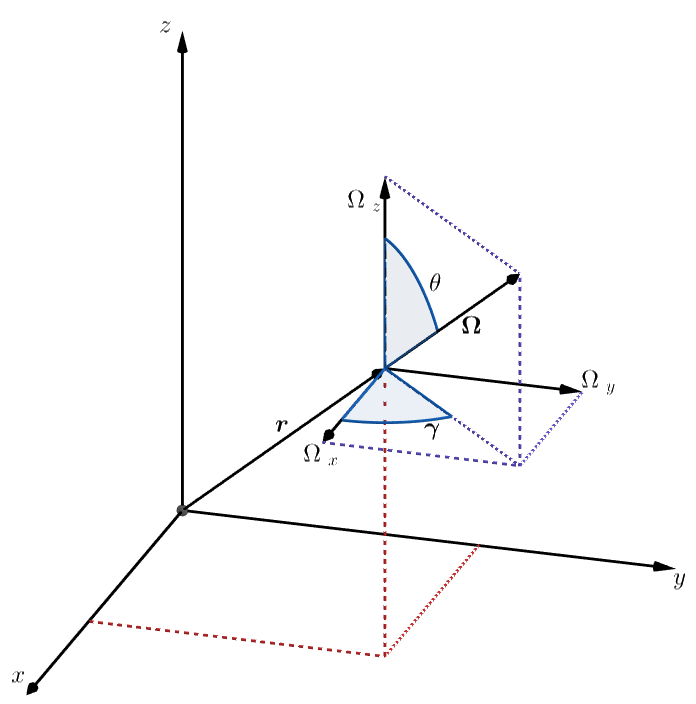
\includegraphics[width=.5\textwidth]{solid_angle2.png} 
		\caption{\label{fig:solid_angle}
			Rectangular Coordinate System}
	\end{figure}

	%From 3D Cartesian geometry, a geometry with no dependence on the $\hat{x}$ and $\hat{y}$ directions, known as 1D slab geometry, can be derived. 
	
	The 3D RT equation \eqref{General_RTg_eqn} can be reduced to 1D slab geometry form where the solution is a function only of the variables $z$ and $\theta$. 1D slab geometry, or plane geometry, is formulated such that the $\hat{x}$ and $\hat{y}$ directions are assumed infinite and material composition does not depend on these directions. Thus the behavior of radiation propagating out in those directions has translational geometry and change is only observed along the $\hat{z}$ axis for different $\pr{\hat{x}, \ \hat{y}}$ planes. The path length $ds$ of propagating radiation can then be written as a function of the distance moved along the $\hat{z}$ axis $(dz)$ and the angle between direction of movement and the $\hat{z}$ axis $\pr{\theta}$
	\begin{equation}
		ds = cos\pr{\theta}dz. \label{ds}
	\end{equation}
	
	\begin{figure}[h]
		\centering
		\captionsetup{justification=centering,margin=2cm}
		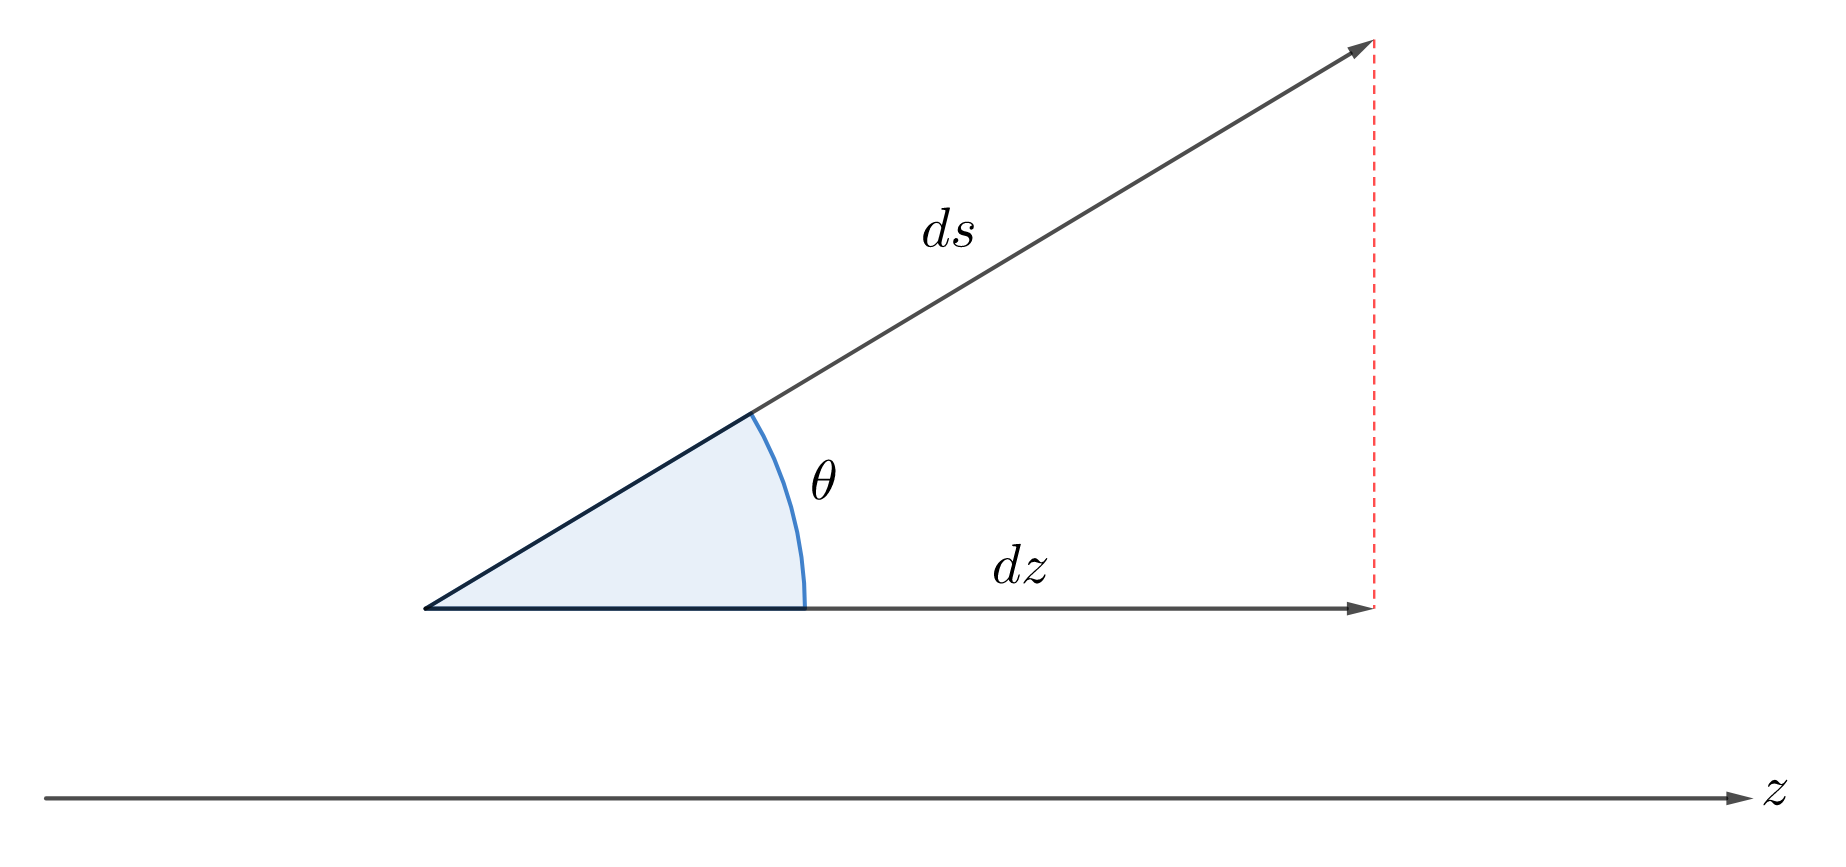
\includegraphics[width=\textwidth]{1dslab.png} 
		\caption{\label{fig:1dslab_geom}
			Path length in 1D slab geometry}
	\end{figure}
	
	Figure \ref{fig:1dslab_geom} depicts the path length described in Eq. \eqref{ds} for 1D slab geometry. The spatial coordinate system \eqref{cartesian} reduces to
	\begin{equation}
		\br = \pr{z}, \quad \grad = \pr{\dz{}}. \label{1d_cartesian}
	\end{equation}
	
	The streaming operator is also reduced by noting $\bOm \cdot \grad \ig = \dv{\ig}{s}$ so that with Eq. \eqref{ds} 
	\begin{equation}
		\bOm \cdot \grad \ig = \dv{\ig}{s} = \dv{\ig}{z}\dv{z}{s} = \dv{\ig}{z}cos\pr{\theta}.
	\end{equation}
	
	The directional cosine is defined as $\mu = cos\pr{\theta}$ so $\bOm \cdot \grad \ig = \mu\cdot\dv{\ig}{z}$. The solution of the RT equation only depends on $z$ and $\mu$ and hence $\ig\pr{\br,\bOm,t} = \ig\pr{z,\mu,t}$. We now integrate the RT equation over $0\leq\gamma\leq 2\pi$ to obtain the 1D slab geometry form of the multigroup RT equation, given by
	\begin{gather}
		\frac{1}{c}\dt{\tilde{I}_g\pr{z,\mu,t}} + \mu\cdot\dx{\tilde{I}_g\pr{z,\mu,t}} + \kapg\pr{T}\tilde{I}_g\pr{z,\mu,t} = 2\pi\kapg\pr{T}\Bg\pr{T}, \label{1D_RTEgz}\\
		0\leq z\leq Z, \quad -1\leq\mu\leq 1, \quad t\geq t_0, \nn
	\end{gather}
	
	where $\tilde{I}_g\pr{z,\mu,t} = 2\pi I_g\pr{z,\mu,t}$ To remain consistent with the usual notation, a notation change is performed such that $\tilde{I}_g\pr{z,\mu,t} \ra I_g\pr{x,\mu,t}$ to rewrite Eq. \eqref{1D_RTEgz} as
	\begin{gather}
		\frac{1}{c}\dt{\ig\pr{x,\mu,t}} + \mu\cdot\dx{\ig\pr{x,\mu,t}} + \kapg\pr{T}\ig\pr{x,\mu,t} = 2\pi\kapg\pr{T}\Bg\pr{T}, \label{1D_RTEg}\\
		0\leq x\leq X, \quad -1\leq\mu\leq 1, \quad t\geq t_0 \nn.
	\end{gather}
	
	Boundary conditions for Eq. \eqref{1D_RTEg} are
	\begin{subequations}
		\begin{align}
			\ig|_{x=0} = \ig^{\text{in},+}\pr{\mu,t}, \quad &\mu>0 \\
			\ig|_{x=X} = \ig^{\text{in},-}\pr{\mu,t}, \quad &\mu<0.
		\end{align}
	\end{subequations}
	
	To discretize the 1D slab geometry RT equation in angle with \textit{discrete-ordinates} a new quadrature set is constructed for $\mu$
	\begin{equation}
		\crl{ \mu_m,\ w_m,\ m=1,\dots ,N_m }
	\end{equation}
	
	where $\mu_m$ are discrete directional cosines specified by the angular mesh and $w_m$ are the corresponding quadrature weights such that
	\begin{equation}
		\sum_{m=1}^{N_m}w_m = 2, \quad \sum_{m=1}^{N_m}\mu_m w_m = 0.
	\end{equation}
	
	Discretizing \eqn{1D_RTEg} with discrete ordinates over angle (Sec. \ref{rte_ang_disc}) and backward-Euler over time (Sec. \ref{rte_time_disc}) yields
	\begin{equation}
		\mu_m\frac{d\igmn\pr{x}}{dx} + \pr{ \kapgn\pr{T} + \frac{1}{c\deltn} }\igmn\pr{x} = \kapgn\pr{T}\Bgn\pr{T} + \frac{\igmnl\pr{x}}{c\deltn}. \label{1D_RTEg_disc}
	\end{equation}	
	
	To discretize the 1D slab geometry RT equation in space a spatial mesh is introduced	
	\begin{equation}
		\crl{ x_{i+\frac{1}{2}}, \quad i=1,\dots ,N_i, \quad 0=x_{\frac{1}{2}}<\dots<x_{i+\frac{1}{2}}<\dots<x_{N_i+\frac{1}{2}}=X }, \label{xmesh}
	\end{equation}
	
	shown in Figure \ref{fig:1Dmesh}. The length of each cell is $\delxi = x_{i+\frac{1}{2}} - x_{i-\frac{1}{2}}$. Cell centers are located at positions $x_i = x_{i-\frac{1}{2}} + \frac{1}{2}\delxi$.
	\begin{figure}[h]
		\centering
		\captionsetup{justification=centering,margin=2cm}
		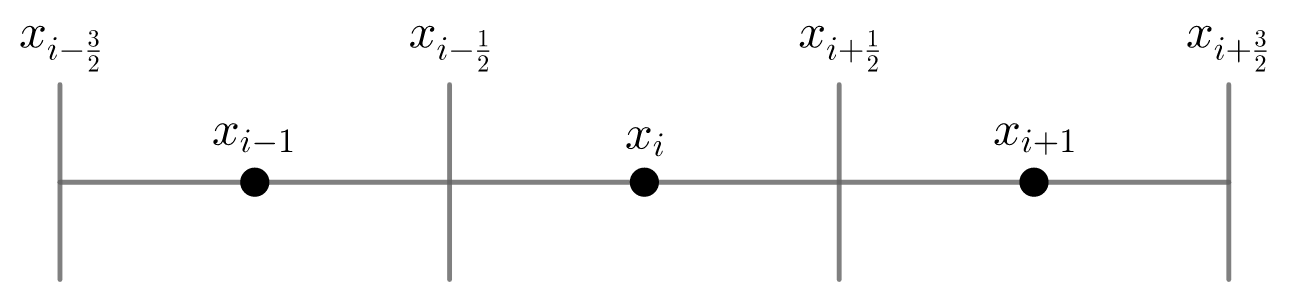
\includegraphics[width=.5\textwidth]{1Dmesh.png}
		\caption{\label{fig:1Dmesh}
			1D spatial mesh grid}
	\end{figure}
	
	%This mesh is designed with the physics of the radiative transfer problem in mind, such that $x_{i+\frac{1}{2}}$ is the right `cell face' and $x_{i-\frac{1}{2}}$ is the left `cell face' of cell $i$. This is done so that the radiation intensity at each `cell face' may be calculated, along with the average intensity per cell. The cell edge radiation intensity is defined as
	
	The discretization scheme formulated on this mesh is known as step characteristics, which follows from the method of characteristics and is defined for cell-average and cell-edge values of the radiation intensity. The radiation intensity at time $t_n$, direction $\mu_m$ and position $x_{i+\frac{1}{2}}$ is written as $\igmirn$. The step characteristics discretization scheme for \eqn{1D_RTEg_disc} for cell-edge radiation intensities is
	\begin{subequations}
		\begin{align}
			&\igmiln = \igmirn e^{-\tau_{g,m,i}} + \frac{Q_{g,m,i,n}}{\modkapgin}\pr{1 - e^{-\tau_{g,m,i}}}, \quad \mu_m > 0\\
			&\igmirn = \igmiln e^{-\tau_{g,m,i}} + \frac{Q_{g,m,i,n}}{\modkapgin}\pr{1 - e^{-\tau_{g,m,i}}}, \quad \mu_m < 0
		\end{align}
		\label{step_edges}
	\end{subequations}
	
	and the equation for cell-average radiation intensities is
	\begin{equation}
		\igmin = \alpha_{g,m,i}\igmiln + \pr{1-\alpha_{g,m,i}}\igmirn, \label{step_avgs}
	\end{equation}
	
	where the source $Q_{g,m,i,n}$ and modified opacity $\modkapgin$ are cell-average quantities given by Eqs. \eqref{modified_source} and \eqref{modified_kap}, respectively. $\tau_{g,m,i}$ is
	\begin{equation}
		\tau_{g,m,i} = \frac{\modkapgin\delxi}{\abs{\mu_m}},
	\end{equation}
	
	and $\alpha_{g,m,i}$ is
	\begin{equation}
		\alpha_{g,m,i} = \left\{ \begin{array}{ll}
			\frac{1}{\tau_{g,m,i}} - \frac{e^{-\tau_{g,m,i}}}{1-e^{-\tau_{g,m,i}}}, & \mu_m>0\\
			-\frac{1}{\tau_{g,m,i}} + \frac{1}{1-e^{-\tau_{g,m,i}}}, & \mu_m<0.
		\end{array} \right.
	\end{equation}
	
%=================================================================================
% DISCRETE MLOQD
%=================================================================================
\section{Discretization of the MLOQD Equations} \label{mloqd_disc}

%=================================================================================
% BACKWARD EULER FOR MLOQD
%=================================================================================
\iffalse
\subsection{Temporal Discretization with Backward-Euler Scheme}
	The backward-Euler temporal discretization scheme applied to the MLOQD Eqs. \eqref{mqd_sys} is
	\begin{subequations}
		\begin{gather}
			\frac{\egn\rdep - \egnl\rdep}{\deltn} + \grad\cdot\bFgn\rdep + c\kapgn\pr{T}\egn\rdep = 4\pi\kapgn\pr{T}\Bgn\pr{T} \label{mqd_1_n}\\
			\frac{1}{c}\frac{\bFgn\rdep - \bFgnl\rdep}{\deltn} + c\grad\cdot\pr{\bfgn\rdep\egn\rdep} + \kapgn\pr{T}\bFgn\rdep = 0 \label{mqd_2_n}
		\end{gather}
	\end{subequations}
	
	where $\egn\rdep$, $\bFgn\rdep$ and $\bfgn\rdep$ are the group radiation energy density, flux and QD factors at time $t_n$.	recombining the terms of Eqs. \eqref{mqd_1_n} and \eqref{mqd_2_n}, respectively gives
	\begin{subequations}
		\begin{gather}
			\grad\cdot\bFgn\rdep + c\pr{\kapgn\pr{T} + \frac{1}{c\deltn}}\egn\rdep = 4\pi\kapgn\pr{T}\Bgn\pr{T} + \frac{\egnl\rdep}{\deltn}  \label{mqd_1_recomb}\\
			c\grad\cdot\pr{\bfgn\rdep\egn\rdep} + \pr{\kapgn\pr{T} + \frac{1}{c\deltn}}\bFgn\rdep = \frac{\bFgnl\rdep}{c\deltn} \label{mqd_2_recomb}
		\end{gather}
		\label{mqd_recombs}
	\end{subequations}
	
	and as seen for the radiative transfer equation in Section \ref{rte_time_disc}, Eqs. \eqref{mqd_recombs} take the form of a steady state multigroup LOQD system with a modified source and opacity
	\begin{subequations}
		\begin{gather}
			\grad\cdot\bFgn\rdep + c\modkapgn\pr{T}\egn\rdep = 4\pi\kapgn\pr{T}\Bgn\pr{T} + \frac{\egnl\rdep}{\deltn}  \label{mqd_1_mod}\\
			c\grad\cdot\pr{\bfgn\rdep\egn\rdep} + \modkapgn\pr{T}\bFgn\rdep = \frac{\bFgnl\rdep}{c\deltn} \label{mqd_2_mod}
		\end{gather}
		\label{mqd_mods}
	\end{subequations}
	
	where the modified opacity is given by \eqn{modified_kap}.
\fi
%=================================================================================
% FINITE VOLUME FOR MLOAM
%=================================================================================
%\subsection{1D Finite Volume}
	The MLOQD equations in 1D slab geometry are
	\begin{subequations}
		\begin{gather}
			\dt{\eg\pr{x,t}} + \dx{\Fg\pr{x,t}} + c\kapg\pr{T}\eg\pr{x,t} = 4\pi\kapg\pr{T}\Bg\pr{T}, \label{mqd_1_1d} \\
			\frac{1}{c}\dt{\Fg\pr{x,t}} + c\dx{\pr{\bfg\pr{x,t}\eg\pr{x,t}}} + \kapg\pr{T}\Fg\pr{x,t} = 0, \label{mqd_2_1d}\\
			0\leq x\leq X, \quad t\geq t_0, \quad g=1,\dots,N_g, \nn
		\end{gather}
		\label{1dmloqd}
	\end{subequations}
	
	with boundary conditions
	\begin{subequations}
		\begin{gather}
			\Fg\pr{0,t} = cC_g^0\pr{t}\pr{\eg\pr{0,t} - E_g^{\text{in},+}\pr{t}} + \Fg^{\text{in},+}\pr{t}, \quad \mu>0\\
			\Fg\pr{X,t} = cC_g^X\pr{t}\pr{\eg\pr{X,t} - E_g^{\text{in},-}\pr{t}} + \Fg^{\text{in},-}\pr{t}, \quad \mu<0
		\end{gather}
	\end{subequations}
	
	where the group boundary factors are
	\begin{align}
		\cgl = \left. \frac{\int_{-1}^{0} \mu\ig d\mu }{\int_{-1}^{0} \ig d\mu} \right|_{x=0}, \quad \cgr = \left. \frac{\int_{0}^{1} \mu\ig d\mu }{\int_{0}^{1} \ig d\mu} \right|_{x=0}.
	\end{align}
	
	The backward-Euler temporal discretization scheme applied to Eqs. \eqref{1dmloqd} is
	\begin{subequations}
		\begin{gather}
			\dx{\Fgn\pr{x}} + c\modkapgn\egn\pr{x} = 4\pi\kapgn\pr{T}\Bgn + \frac{\egnl\pr{x}}{\deltn},  \label{mqd_1_1dn}\\
			c\dx{\pr{\fgn\pr{x}\egn\pr{x}}} + \modkapgn\Fgn\pr{x} = \frac{\Fgnl\pr{x}}{c\deltn} \label{mqd_2_1dn},
		\end{gather}
	\end{subequations}
	
	%We consider the spatial mesh \eqref{xmesh} as shown in Figure \ref{fig:1Dmesh} for spatial discretization. The aim of this discretization is to find a system of equations in terms of the `cell-edge' radiation fluxes and `cell-average' radiation energy densities. This is based on the units of each of these quantities, since the radiation flux is the intensity of radiation moving through a plane and the radiation energy density is the intensity of radiation present in a given volume. 
	
	A second-order finite volume scheme is used to disctretize the MLOQD system in space. The radiation energy balance \eqn{mqd_1_1dn} is integrated over the spatial interval of the $i^{th}$ cell $x_{i-\frac{1}{2}}\leq x\leq x_{i+\frac{1}{2}}$ to give
	\begin{equation}
		\Fgirn - \Fgiln + c\delxi\modkapgin\egin = \delxi\pr{4\pi\kapgin\Bgin + \frac{\eginl}{\deltn}}, \label{mqd_1_disc}
	\end{equation}
	
	where $\Fgirn$ is the cell-edge value of the group-wise radiation flux and $\egin$ is the cell-averaged value of the group-wise radiation energy density. The radiation momentum balance \eqn{mqd_2_1dn} is integrated over the the $i^{th}$ cell's left half $x_{i-\frac{1}{2}}\leq x\leq x_{i}$ and over its right half $x_{i}\leq x\leq x_{i+\frac{1}{2}}$. This gives two discretized equations
	\begin{gather}
		c\pr{\fgin\egin - \fgiln\egiln} + \frac{\delxi}{2}\modkapgin\Fgiln = \frac{\delxi}{2}\frac{\Fgilnl}{c\deltn}, \label{mloqd_disc_left}\\
		c\pr{\fgirn\egirn - \fgin\egin} + \frac{\delxi}{2}\modkapgin\Fgirn = \frac{\delxi}{2}\frac{\Fgirnl}{c\deltn} \label{mloqd_disc_right}.
	\end{gather}
	
	To eliminate the cell-edge radiation energy density $\egirn$, \eqn{mloqd_disc_left} is found for the $i+1$ cell and combined with \eqn{mloqd_disc_right} to obtain
	\begin{equation}
		c\pr{\fgirrn\egirrn - \fgin\egin} + \delxir\modkapgirn\Fgirn = \delxir\frac{\Fgirnl}{c\deltn}, \label{mqd_2_disc}
	\end{equation}
	
	where
	\begin{equation}
		\delxir = \frac{\delxi + \delxirr}{2},
	\end{equation}
	
	with $\Delta x_0=0$, $\Delta x_{I+1}=0$, and the cell-edge opacity is
	\begin{equation}
		\kapgirn = \frac{\delxi\kapgin+\delxirr\kapgirrn}{\delxi+\delxirr}, \ \ \modkapgirn = \frac{\delxi\modkapgin+\delxirr\modkapgirrn}{\delxi+\delxirr}.
	\end{equation}
	
	The discrete MLOQD system is thus
	\begin{subequations}
		\begin{gather}
			\Fgirn - \Fgiln + c\delxi\modkapgin\egin = \delxi\pr{4\pi\kapgin\Bgin + \frac{\eginl}{\deltn}} \label{mqd_1_disc_2},\\
			c\pr{\fgirrn\egirrn - \fgin\egin} + \delxir\modkapgirn\Fgirn = \delxir\frac{\Fgirnl}{c\deltn} \label{mqd_2_disc_2}.
		\end{gather}
		\label{mqd_sys_disc}
	\end{subequations}
	
	The discretized MLOQD Eqs. \eqref{mqd_sys_disc} give a system of equations for the group radiation flux and energy density. Eqs. \eqref{mqd_sys_disc} can be manipulated to eliminate the group radiation flux and create a smaller linear system, demonstrated for the GLOQD system in Sec. (\ref{sec:gloqd_disc}).
	
%=================================================================================
% DISCRETE GLOQD
%=================================================================================
\section{Discretization of the GLOQD and MEB Equations} \label{sec:gloqd_disc}

%=================================================================================
% BACKWARD EULER FOR GLOQD
%=================================================================================
%\subsection{Discretization of the GLOQD and MEB Equations} \label{gloqd_disc}
	To maintain algebraic consistency between the discretization of the MLOQD equations and the GLOQD equations, the discrete GLOQD equations are derived from the discrete MLOQD Eqs. \eqref{mqd_sys_disc} by summing them over group. The discrete GLOQD equations are thus
	\begin{subequations}
	\begin{equation}
		\Fbirn - \Fbiln + c\delxi\modkapebin\ebin = \delxi\pr{c\kapbbin\ar T^4_{i,n} + \frac{\ebinl}{\deltn}}, \label{gqd_1_disc}
	\end{equation}
	\vspace*{-1cm}
	\begin{multline}
		c\pr{\fbirrn+\etairnp}\ebirrn - c\pr{\fbin+\etairnm}\ebin \\+ \delxir\modkaprbirn\Fbirn = \delxir\frac{\Fbirnl}{c\deltn}. \label{gqd_2_disc}
	\end{multline}
	\label{gqd_sys_disc}
	\end{subequations}
	
	where the total cell-averaged radiation energy density is
	\begin{equation}
		\ebin = \sum_{g=1}^{N_g}\egin,
	\end{equation}
	
	and the total cell face averaged radiation flux is
	\begin{equation}
		\Fbirn = \sum_{g=1}^{N_g}\Fgirn.
	\end{equation}
	
	The group QD factor in each cell is averaged with the cell-averaged group energy density to form the cell-averaged grey QD factor
	\begin{equation}
		\fbin = \frac{\sum_{g=1}^{N_g} \fgin\egin}{\sum_{g=1}^{N_g} \egin}.
	\end{equation}
	
	The two modified grey opacities are
	\begin{gather}
		\modkapebin = \kapebin + \frac{1}{c\deltn}, \label{modkapE} \\
		\modkaprbirn = \kaprbirn + \frac{1}{c\deltn},
	\end{gather}
	
	and the three distinct grey opacities in each cell or cell face are
	\begin{gather}
		\kapebin = \frac{ \sum_{g=1}^{N_g}\kapgin\egin }{ \sum_{g=1}^{N_g}\egin }, \\[5pt]
		\kapbbin = \frac{ \sum_{g=1}^{N_g}\kapgin\Bgin }{ \sum_{g=1}^{N_g}\Bgin }, \\[5pt]
		\kaprbirn = \frac{ \sum_{g=1}^{N_g}\kapgirn\abs{\Fgirn} }{ \sum_{g=1}^{N_g}\abs{\Fgirn} }.
	\end{gather}
	
	The compensation term takes the form
	\begin{subequations}
		\begin{align}
			&\etairn = \sum_{g=1}^{N_g} \brk{\pr{\kapgirn - \kaprbirn}\Fgirn},\\
			&\etairnp = \left\{ \begin{array}{ll}
							\frac{\etairn}{\sum_{g=1}^{N_g} \egirrn}, & \etairn>0,\\
							0, & \etairn<0,
						\end{array} \right.\\
			&\etairnm = \left\{ \begin{array}{ll}
							0, & \etairn>0,\\
							\frac{-\etairn}{\sum_{g=1}^{N_g} \egin}, & \etairn<0.
						\end{array} \right.
		\end{align}
	\end{subequations}
	
	The terms $\eta^{\pm}$ are defined as such so that the coefficient multiplying the total radiation energy density in the radiation momentum balance Eq. \eqref{gqd_2_disc} does not become negative. The discretized GLOQD Eqs. \eqref{gqd_sys_disc} give a system of equations for the total radiation flux and energy density. %One may eliminate the total radiation flux from \eqn{gqd_1_disc} by using \eqn{gqd_2_disc} to substitute and create a smaller linear system to solve for only the cell-average total radiation energy density.
	
	\ind Now considering the MEB equation \eqref{Energy_Balance_gr}, the 1D slab geometry form is
	\begin{equation}
		\dt{\varepsilon\pr{T}} = c\kapeb\pr{T}\eb\pr{x,t} - c\kapbb\pr{T}\ar T^4. \label{Energy_Balance_gr2}
	\end{equation}
	
	%One can make the assumption that the material energy density $\varepsilon\pr{T}$ is simply the specific heat of the material $\cv$ times the material temperature $T$
	%\begin{equation}
	%	\varepsilon\pr{T} = \cv T,
	%\end{equation}
	
	%which gives a new form of the MEB equation
	%\begin{equation}
	%	\cv\dt{T} = c\kapeb\pr{T}\eb\pr{x,t} - c\kapbb\pr{T}\ar T^4. \label{Energy_Balance_gr3}
	%\end{equation}
	
	\eqn{Energy_Balance_gr2} then takes on the discrete form
	\begin{equation}
	%	\cv\frac{\tin - \tinl}{\delt} = c\kapebin\ebin - c\ar\kapbbin\tin^4. \label{ebdisc}
		\frac{\varepsilon_{i,n}\pr{T} - \varepsilon_{i,n-1}\pr{T}}{\delt_n} = c\kapebin\ebin - c\ar\kapbbin\tin^4. \label{ebdisc}
	\end{equation}
	
	The GLOQD equations \eqref{gqd_sys_disc} share a source term with the MEB Eq. \eqref{ebdisc}
	\begin{equation}
		\qbin = c\ar\kapbbin\tin^4. \label{grsource}
	\end{equation}
	
%\subsection{Removing the Radiation Flux from the Effective Grey Problem \label{Fremove}}
	A reduced system is derived from the GLOQD \eqref{gqd_sys_disc} and MEB \eqref{ebdisc} equations by eliminating the total radiation flux. The terms of the grey radiation momentum balance Eq. \eqref{gqd_2_disc} are recombined as
	\begin{equation}
		\Fbirn = \bar{h}_i - \Dirnp\ebirrn + \Dirnm\ebin, \label{Fisolate}
	\end{equation}
	
	where
	\begin{gather}
		\bar{h}_i = \frac{\Fbirnl}{c\delt\kaprbirn+1}, \\
		\Dirnp = \frac{c\fbirrn + \etairnp}{\delxir\modkaprbirn}, \\
		\Dirnm = \frac{c\fbin + \etairnm}{\delxir\modkaprbirn}.
	\end{gather}
	
	%$\Fbirn$ and $\Fbiln$ in Eq. \eqref{gqd_1_disc} are replaced with Eq. \eqref{Fisolate} to give
	%\begin{multline}
	%	\pr{- \Dirnp\ebirrn + \Dirnm\ebin} - \pr{- \Dilnp\ebin + \Dilnm\ebilln} + c\delx\modkapebin\ebin \\= \delx\qbin + \frac{\delx\ebinl}{\delt} - \bar{h}_i + \bar{h}_{i-1}.
	%\end{multline}
	
	$\Fbirn$ and $\Fbiln$ in Eq. \eqref{gqd_1_disc} are replaced with Eq. \eqref{Fisolate} to give the discrete system of GLOQD and MEB equations
	\begin{subequations}
		\begin{multline}
			- \Dilnm\ebilln + \pr{\Dirnm + \Dilnp + c\delx\modkapebin}\ebin - \Dirnp\ebirrn \\ = \delx\qbin + P_{i,n-\frac{1}{2}}, \label{gqd_E}
		\end{multline}
		\vspace*{-.5cm}
		\begin{equation}
			\frac{\varepsilon_{i,n} - \varepsilon_{i,n-1}}{\delt_n} = c\kapebin\ebin - \qbin, \label{ebdisc2}
		\end{equation}
		\label{reduced_gr_sys}
	\end{subequations}

	with Eq. \eqref{Fisolate} as an auxiliary used to calculate radiation flux values from the solution of \eqref{reduced_gr_sys} and
	\begin{equation}
		P_{i,n-\frac{1}{2}} = \frac{\delx_i\ebinl}{\delt_n} + \bar{h}_{i-1} - \bar{h}_{i}.
	\end{equation}
	
	
	
%=================================================================================
% 
%=================================================================================
%\section{The QD System}
%	The full system of equations used in the QD method contains the RT, multigroup LOQD and grey LOQD Eqs. \eqref{step_edges}, \eqref{step_avgs}, \eqref{mqd_sys_disc} \& \eqref{gqd_sys_disc}.
	%\begin{subequations}
	%	\begin{gather}
	%		
	%	\end{gather}
	%\end{subequations}

%=================================================================================
% Coupling the Grey low-order and Energy Balance Equations
%=================================================================================
\section{Newton's Method for the GLOQD and MEB Equations} \label{sec:newton}
	Newton's method \cite{kelley-newton} is used to solve the GLOQD and MEB Eqs. \eqref{reduced_gr_sys}. It is an iterative method to find the roots of a given system of nonlinear equations
	\begin{equation}
		\bm{G}\pr{\bx} = 0. \label{Gdef}
	\end{equation}
	
	The system of equations is linearized about some estimate of the solution to obtain
	\begin{equation}
		\bm{G}\pr{\bx^{\pr{s}}} + \bm{G}'\pr{\bx^{\pr{s}}}\pr{\bx-\bx^{\pr{s}}} = 0, \label{linear}
	\end{equation}
	
	where $\bG'$ is the Jacobian of the system, and $\bx^{\pr{s}}$ is the solution of the $s^{\text{th}}$ iterate. Eq. \eqref{linear} is then rewritten as
	\begin{equation}
		\Delta \bx^{\pr{s}} =  - \pr{\bG'\pr{\bx^{\pr{s}}}}^{-1}\bm{G}\pr{\bx^{\pr{s}}},
	\end{equation}
	
	where $\Delta \bx^{\pr{s}} = \bx-\bx^{\pr{s}}$. The solution of the following iterate is defined as
	\begin{equation}
		\bx^{\pr{s+1}} = \bx^{\pr{s}} + \Delta \bx^{\pr{s}},
	\end{equation}
	
	thus
	\begin{equation}
		\bx^{\pr{s+1}} = \bx^{\pr{s}} - \pr{\bG'\pr{\bx^{\pr{s}}}}^{-1}\bm{G}\pr{\bx^{\pr{s}}}.
	\end{equation}
	
	The discretized GLOQD and MEB Eqs. \eqref{reduced_gr_sys} form a system for the total radiation energy density and temperature vectors $\pr{\bE,\bT}$. We define
	\begin{gather}
		\ebinsrv = \ebinsv + \debinsv \label{dele}\\
		\tinsrv = \tinsv + \dtinsv, \label{delt}
	\end{gather}
	
	where $\debinsv$ and $\dtinsv$ are the iterative increments for the radiation energy density and temperature, respectively. The grey functions that depend on temperature are also linearized, namely the opacity $(\kapeb)$, material energy density $(\varepsilon)$ and source term $(\qb)$ to get
	\begin{gather}
		\varepsilon_{i,n}^{\pr{s+1}} = \varepsilon_{i,n}^{\pr{s}} + \frac{d\varepsilon_{i,n}^{\pr{s}}}{dT}\dtinsv,\\
		\qbinsrv = \qbinsv + \frac{d\qbinsv}{dT}\dtinsv, \\
		%\kapebin^{\pr{s+1}} = \kapebin^{\pr{s}} + \dv{\kapebin^{\pr{s}}}{T}\dtinsv,\\
		\kapebin^{\pr{s+1}} = \kapebin^{\pr{s}} + \pr{\fd \kapebin}^{\pr{\ell}}\dtinsv. \label{frechet}
	\end{gather}
	
	The source term and material energy density are known local functions of temperature and thus their derivatives with respect to $T$ can be directly calculated. The opacity $\kapeb$ however, is an averaged quantity over the entire spectrum range. Thus the grey opacity depends not only on the change in the multi-group opacity, but also on the spectrum change and is thus globally dependent on temperature. The Fr\'echet derivative $\pr{\fd \kapebin}^{\pr{\ell}}$ must be approximated to take into account the variation in energy density spectrum. Here $\ell$ denotes the index of the MLOQD iteration. This Fr\'echet derivative is calculated using the value of the grey opacity and temperature at successive MLOQD iterations
	\begin{equation}
		\pr{\fd \kapebin}^{\pr{\ell}} = \frac{\kapebin^{\pr{\ell}} - \kapebin^{\pr{\ell-1}}}{\tin^{\pr{\ell}} - \tin^{\pr{\ell-1}}}, \label{frachet2}
	\end{equation}
	
	The use of Eqs. \eqref{frechet} and \eqref{frachet2} lead to an approximate Jacobian. Substituting the linearized quantities for $\ebinsrv$, $\tinsrv$, $\varepsilon_{i,n}^{\pr{s+1}}$, $\qbinsrv$ and $\kapebin^{\pr{s+1}}$ into Eq. \eqref{gqd_E} yields
	\begin{multline}
		 - \Dilnm\pr{\ebilnsv + \debillnsv} \\+ \pr{\Dirnm + \Dilnp + c\delx\pr{\kapebin^{\tau\pr{s}} + \pr{\fd \kapebin^{\tau}}^{\pr{\ell}}\dtinsv}}\pr{\ebinsv + \debinsv} \\- \Dirnp\pr{\ebirnsv + \debirrnsv}= \delx\pr{\qbinsv + \frac{d\qbinsv}{dT}\dtinsv} + P_{i,n-\frac{1}{2}},
	\end{multline}
	
	which is reformed as
	\begin{multline}
		- \Dilnm\debillnsv + \pr{\Dirnm + \Dilnp + c\delxi\kapebin^{\tau\pr{s}}}\debinsv - \Dirnp\debirrnsv \\
		+\pr{ c\delxi \pr{\fd \kapebin^{\tau}}^{\pr{\ell}}\ebinsv- \delxi \frac{d\qbinsv}{dT}}\dtinsv = -R_{E,i}^{\pr{s}}, \label{delE_eq}
	\end{multline}
	
	where second order $\Delta T \Delta E$ terms have been neglected and 
	\begin{multline}
		R_{E,i}^{\pr{s}} = - \Dilnm\ebilnsv + \pr{\Dirnm + \Dilnp + c\delxi\kapebin^{\tau\pr{s}}}\ebinsv \\ - \Dirnp\ebirnsv - \delxi \qbinsv - P_{i,n-\frac{1}{2}} \label{Eres}
	\end{multline}
	
	is the residual of Eq. \eqref{gqd_E}. The linearized quantities are also substituted into Eq. \eqref{ebdisc2}
	\begin{multline}
		\frac{1}{\delt_n}\pr{\varepsilon_{i,n}^{\pr{s}} + \frac{d\varepsilon_{i,n}^{\pr{s}}}{dT}\dtinsv - \varepsilon_{i,n-1}}\\ = c\pr{\kapebin^{\pr{s}} + \pr{\fd \kapebin^{\tau}}^{\pr{\ell}}\dtinsv}\pr{\ebinsv + \debinsv} - \qbinsv - \frac{d\qbinsv}{dT}\dtinsv,
	\end{multline}
	
	and solving for $\dtinsv$ yields
	\begin{align}
		\dtinsv = \xi_{i}^{\pr{s}-1}\pr{c\kapebin^{\pr{s}}\debinsv - R_{T,i}^{\pr{s}}}, \label{del_T_eqn}
	\end{align}
	
	where
	\begin{equation}
		\xi_{i}^{\pr{s}} = \frac{1}{\delt_n}\frac{d\varepsilon_{i,n}^{\pr{s}}}{dT} - c\pr{\fd \kapebin^{\tau}}^{\pr{\ell}}\ebinsv + \frac{d\qbinsv}{dT}
	\end{equation}
	
	and 
	\begin{equation}
		R_{T,i}^{\pr{s}} = \frac{\varepsilon_{i,n}^{\pr{s}} - \varepsilon_{i,n-1}}{\delt_n} - c\kapebin^{\pr{s}}\ebinsv + \qbinsv
	\end{equation}
	
	is the residual of Eq. \eqref{ebdisc2}. An equation only in terms of $\Delta E$ is derived by combining Eqs. \eqref{delE_eq} and \eqref{del_T_eqn} 
	\begin{multline}
		- \Dilnm\debillnsv + \pr{\Dirnm + \Dilnp + c\delxi\kapebin^{\tau\pr{s}}}\debinsv - \Dirnp\debirrnsv \\ +\pr{ c\delxi \pr{\fd \kapebin^{\tau}}^{\pr{\ell}}\ebinsv- \delxi \frac{d\qbinsv}{dT}}\pr{\xi_{i}^{\pr{s}-1}\pr{c\kapebin^{\pr{s}}\debinsv - R_{T,i}^{\pr{s}}}} = -R_{E,i}^{\pr{s}}, \label{delE_eq2}
	\end{multline}
	
	rewritten in the condensed form
	\begin{equation}
		- \Dilnm\debillnsv + \bar{\zeta}_{i}\debinsv - \Dirnp\debirrnsv =  R_{E/T,i}^{\pr{s}}, \label{delE_cond}
	\end{equation}
	
	with
	\begin{equation}
		\bar{\zeta}_{i} = \Dirnm + \Dilnp + c\delxi\kapebin^{\tau\pr{s}} \\+ \frac{c\kapebin^{\pr{s}}}{\xi_{i}^{\pr{s}}}\pr{ c\delxi \pr{\fd \kapebin^{\tau}}^{\pr{\ell}}\ebinsv- \delxi \frac{d\qbinsv}{dT}},
	\end{equation}
	%\vspace*{-1cm}	
	\begin{equation}
		R_{E/T,i}^{\pr{s}} = -R_{E,i}^{\pr{s}} + \frac{R_{T,i}^{\pr{s}}}{\xi_{i}^{\pr{s}}}\pr{c\delxi \pr{\fd \kapebin^{\tau}}^{\pr{\ell}}\ebinsv- \delxi \frac{d\qbinsv}{dT}}.
	\end{equation}
	
	The GLOQD and MEB system is solved for $\Delta \bE$ with Eq. \eqref{delE_cond}, and this solution is used in Eq. \eqref{del_T_eqn} to find $\Delta \bT$. Then Eqs. \eqref{dele} and \eqref{delt} are used to find $\bE$ and $\bT$.
	
\section{Summary of the Discrete MLQD Formulation}
	The discrete MLQD set of equations consists of:
	\begin{itemize}
		\item The step-characteristics form of the RT equation for cell-edge intensities \eqref{step_edges} and cell-average intensities \eqref{step_avgs},
		\item The discrete multigroup LOQD system \eqref{mqd_sys_disc} for the group radiation energy density and flux,
		\item The discrete grey LOQD and MEB Eqs. \eqref{delE_cond}, \eqref{del_T_eqn}, \eqref{dele}, \eqref{delt} \& \eqref{Fisolate} for the total radiation energy density and flux and material temperature.
	\end{itemize}

	The nonlinear multilevel iterative process to solve the discretized MLQD system is depicted in algorithm \ref{alg:mlqd_alg_full}. There are three nested iterative loops that successively solve the RT equation, multigroup LOQD system and the grey LOQD and MEB system. This algorithm shares the same properties as discussed for algorithm \ref{alg:mlqd_alg} in section \ref{sec:qd_roms}.
	
	\begin{algorithm}[ht!]
		\SetAlgoLined
		\While{$t_n \leq t^{\text{end}}$}{
			$n=n+1$\\
			$\bT^{\pr{0}} = \bT_{n-1}$\\
			\While{$\norm{\bT^{\pr{w}}-\bT^{\pr{w-1}}} > \epsilon_1\norm{\bT^{\pr{w}}} + \epsilon_2, \ \ \norm{\bE^{\pr{w}}-\bE^{\pr{w-1}}} > \epsilon_1\norm{\bE^{\pr{w}}} + \epsilon_2 $}{
				$w=w+1$\\
				Solve multigroup RT Eqs. \eqref{step_edges} \& \eqref{step_avgs} for $\bm{I}_{g}^{\pr{w}}$\\
				Compute group QD factors $\bfg^{\pr{w}}$\\
				\While{$\norm{\bT^{\pr{\ell,w}}-\bT^{\pr{\ell-1,w}}} > \tilde{\epsilon}_1\norm{\bT^{\pr{\ell,w}}} + \tilde{\epsilon}_2, \ \ \norm{\bE^{\pr{\ell,w}}-\bE^{\pr{\ell-1,w}}} > \tilde{\epsilon}_1\norm{\bE^{\pr{\ell,w}}} + \tilde{\epsilon}_2 $}{
					$\ell=\ell+1$ \\
					Solve multigroup LOQD eqs. \eqref{mqd_sys_disc} for $\bm{E}_{g}^{\pr{\ell,w}}$ and $\bm{F}_{g}^{\pr{\ell,w}}$\\
					Compute grey quantities $\kapeb^{\pr{\ell,w}}$, $\kapbb^{\pr{\ell,w}}$, $\kaprb^{\pr{\ell,w}}$, $\bfb^{\pr{\ell,w}}$, $\etab^{\pr{\ell,w}}$, $\frac{d \kapebin}{d T}^{\pr{\ell}}$\\
					\While{$\norm{\bT^{\pr{s,\ell,w}}-\bT^{\pr{s-1,\ell,w}}} > \tilde{\epsilon}_1\norm{\bT^{\pr{s,\ell,w}}} + \tilde{\epsilon}_2, \ \ \norm{\bE^{\pr{s,\ell,w}}-\bE^{\pr{s-1,\ell,w}}} > \tilde{\epsilon}_1\norm{\bE^{\pr{s,\ell,w}}} + \tilde{\epsilon}_2 $}{
						Solve Eqs. \eqref{delE_cond} \& \eqref{del_T_eqn} for $\Delta \bE^{\pr{s}}$ and $\Delta \bT^{\pr{s}}$ \\
						$\bE^{\pr{s,\ell,w}} = \bE^{\pr{s-1,\ell,w}} + \Delta \bE^{\pr{s}} \ ; \ \bT^{\pr{s,\ell,w}} = \bT^{\pr{s-1,\ell,w}} + \Delta \bT^{\pr{s}}$ \\
						Solve Eq. \eqref{Fisolate} for $\bm{F}^{\pr{s,\ell,w}}$
					}
					$\bT^{\pr{\ell,w}} \leftarrow \bT^{\pr{s,\ell,w}}$\\
					Update opacities $\kapg\pr{\bT^{\pr{\ell,w}}}$
				}
				$\bT^{\pr{w}} \leftarrow T^{\pr{\ell,w}}$
			}
			$\bT_n \leftarrow \bT^{\pr{w}}$
		}
		\caption{Iterative scheme for the MLQD method in discrete form \label{alg:mlqd_alg_full}}
	\end{algorithm}
	
	
	
\chapter{A ROM Based on the Multigroup LOQD Equations and Proper Orthogonal Decomposition of QD Factors}
\label{chap-three}

This chapter develops a ROM for solving TRT problems based on the hierarchy of LOQD equations using the POD (Sec. \ref{sec:pod}) to estimate group QD factors \cite{jc-dya-m&c2019}. Sections \ref{sec:pod-qd} and \ref{sec:mpod_test} formulate this ROM and the problem used to test its performance. Section \ref{sec:reduced_qdf} analyses the POD of the group QD factors, and section \ref{sec:mloqd-pod_res} describes the numerical results of this ROM.

%=================================================================================
% POD-BASED REPRESENTATION  OF GROUP QD FACTORS
%=================================================================================
\section{Formulation of the MLOQD-POD ROM} \label{sec:pod-qd} 
	The POD methodology is applied to the grid function of QD factors $f_g(x_i,t_n)$. The QD factors are defined on grids of energy, space and time, and the POD is applied to each energy group separately to obtain approximations over space and time. First a database of known QD factors is created by solving the TRT problem with the MLQD method to generate a solution on some mesh in space and time \cite{dya-jcp-2019,dya-aristova-vya-mm1996,PASE-1986}. The QD factors are formed into $N_g$ group-wise matrices $\bA^{f}_g \in \real^{\chi,\tau}$ where each matrix holds the set of QD factors for a particular energy group $g$. Each column in $\bA^f_g$ contains the spatial vector of QD factors at a separate instant of time (snapshots), ordered chronologically. The SVD  is applied to each $\bA^f_g$ to cast in the form of \eqn{svd_form}, $\bA^f_g = \bU_g\bSig_g\bV_g^T$ where $\bU_g \in \real^{\chi,k}$, $\bSig_g \in \real^{k,k}$, $\bV_g \in \real^{\tau,k}$, and $k = \min\pr{\chi,\tau}$. Each group database is approximated separately as a reduced rank matrix of rank $r_g \leq k$, satisfying some value for the singular value relative cutoff criteria (Eq. \ref{cutoff_eps}). The reduced rank approximation of each group QD factor matrix is thus given as $\bA^{f*}_g  = \bU_g^*\bSig_g^*\pr{\bV^{*}_g}^T $ where $\bU_g^* \in \real^{\chi,r_g}$, $\bSig_g^* \in \real^{r_g,r_g}$, $\bV_g^{*T} \in \real^{r_g,\tau}$.
	
	%%%%%%%%%%%%%%%%%%%%%%%%%%%%%%%%%%%%%%%
	\iffalse
	A singular value relative cutoff criteria is defined $\varepsilon_\sigma < 1$ such that for each set of singular values per group, $(\sigma_{1,g},\dots,\sigma_{k,g})$, there will be a $r_g \leq k$ such that
	\begin{equation}
		\frac{\sigma_{n,g}}{\sigma_{1,g}} \geq \varepsilon_\sigma \label{cutoff_eps2}
	\end{equation}
	
	for all $n \leq r_g$. The reduced rank approximation of each group QD factor matrix is thus given as $\bA^{f*}_g  = \bU_g^*\bSig_g^*\bV_g^{*T} $ where $\bU_g^* \in \real^{\chi,r_g}$, $\bSig_g^* \in \real^{r_g,r_g}$, $\bV_g^{*T} \in \real^{r_g,\tau}$. The ratio of energy contained in the first $n$ POD modes to the total energy of all POD modes \cite{Benner-siam-2015} is
	\begin{equation}
		\gamma_n = \frac{\sum_{i=1}^{n} \sigma_i^2}{\sum_{i=1}^{k} \sigma_i^2}, \label{worth_gam2}
	\end{equation}
	This can also be interpreted as the ratio of modeled to total energy contained in the data snapshots \cite{gubisch-volkwein}.
	\fi
	%%%%%%%%%%%%%%%%%%%%%%%%%%%%%%%%%%%%%%%
	
	\ind This ROM uses approximate QD factors $\fg^*$ computed by means of a low-rank SVD of $\bA_g^f$ to define an approximate closure to the system of MLOQD Eqs. \eqref{mqd_sys}. The ROM is defined by the resulting multigroup low-order equations
	\begin{subequations}
		\begin{gather}
			\dt{\eg\pr{x,t}} + \dx{\bFg\pr{x,t}} + c\kapg\pr{T}\eg\pr{x,t} = 4\pi\kapg\pr{T}\Bg\pr{T}, \label{mlqd_pod_zero}\\
			\frac{1}{c}\dt{\bFg\pr{x,t}} + c\dx{\fg^*\pr{x,t}\eg\pr{x,t}} + \kapg\pr{T}\bFg\pr{x,t} = 0, \label{mlqd_pod_first}
		\end{gather}
			\label{mlqd_pod_eqs}
	\end{subequations}

	
	\iffalse
	\begin{subequations}
		\begin{gather}
			\dt{\eb\pr{x,t}} + \dx{\bFb\pr{x,t}} + c\kapeb\pr{T}\eg\pr{x,t} = 4\pi\kapbb\pr{T}\Bg\pr{T} \label{mlqd_pod_zero_gr}\\
			\frac{1}{c}\dt{\bFb\pr{x,t}} + c\dx{\fb^*\pr{x,t}\eb\pr{x,t}} + \kaprb\pr{T}\bFg\pr{x,t} + \eta\pr{x,t}\eb\pr{x,t} = 0, \label{mlqd_pod_first_gr}
		\end{gather}
			\label{mlqd_pod_gr_eqs}
	\end{subequations}

	and material energy balance equation
	\begin{equation}
		\dt{\varepsilon\pr{T}} = c\kapeb\pr{T}\eb\pr{x,t} - c\kapbb\pr{T}\ar T^4. \label{mlqd_pod_eb}
	\end{equation}
	\fi
	
	GLOQD equations \eqref{gqd_sys}, and MEB equation \eqref{Energy_Balance_gr}. The grey QD factor computed with $\fg^*$ is
	\begin{equation}
		\fb^*\pr{x,t} = \frac{\sum_{g=1}^{N_g} \fg^*\pr{x,t}\eg\pr{x,t}}{\sum_{g=1}^{N_g} \eg\pr{x,t}},
	\end{equation}
	
	\iffalse
	the grey opacities are
	\begin{subequations}
		\begin{gather}
			\kapeb\pr{T} = \frac{ \sum_{g=1}^{N_g}\kapg\pr{T}\eg\pr{x,t} }{ \sum_{g=1}^{N_g}\eg\pr{x,t} } \\[5pt]
			\kapbb\pr{T} = \frac{ \sum_{g=1}^{N_g}\kapg\pr{T}\Bg\pr{T} }{ \sum_{g=1}^{N_g}\Bg\pr{T} } \\[5pt]
			\kaprb\pr{T} = \frac{ \sum_{g=1}^{N_g}\kapg\pr{T}\abs{\bFg\pr{x,t}} }{ \sum_{g=1}^{N_g}\abs{\bFg\pr{x,t}} },
		\end{gather}
		\label{mlqd_pod_grey_opacities}
	\end{subequations}

	and the compensation term is
	\begin{equation}
		\eta\pr{x,t} = \frac{ \sum_{g=1}^{N_g}\brk{\pr{\kapg\pr{T} - \kaprb\pr{T}}\bFg\pr{x,t}} }{ \sum_{g=1}^{N_g}\eg\pr{x,t} }.
	\end{equation}
	\fi
	
	
	\iffalse
	\begin{subequations}
			\begin{gather}
				\Fgirn - \Fgiln + c\delxi\modkapgin\pr{T}\egin = \delxi\pr{4\pi\kapgin\pr{T}\Bgin\pr{T} + \frac{\eginl}{\deltn}}\\
				c\pr{\fgirrn^*\egirrn - \fgin^*\egin} + \delxir\modkapgirn\pr{T}\Fgirn = \delxir\frac{\Fgirnl}{c\deltn}\\
				\Fbirn - \Fbiln + c\delxi\kapebin^*\pr{T}\ebin = c\kapbbin\pr{T}\ar T^4_{i,n} + \frac{\ebinl}{\deltn}
			\end{gather}
			\vspace*{-1.2cm}
			\begin{multline}
				c\pr{\fbirrn^*\ebirrn - \fbin^*\ebin} + \delxir\modkaprbirn\pr{T}\Fbirn \\+ \pr{\etairnp\ebirrn - \etairnm\ebin} = \delxir\frac{\Fbirnl}{c\deltn}
			\end{multline}
			\vspace*{-.9cm}
			\begin{gather}
				\frac{\varepsilon_{i,n}\pr{T} - \varepsilon_{i,n-1}\pr{T}}{\delt_n} = c\kapebin\ebin - c\ar\kapbbin\tin^4\\
				i = 1,\dots,I, \ g = 1,\dots,N_g, \ n = 1,\dots,N_n \nn
			\end{gather}
	\end{subequations}
	\fi

	The discrete form of this ROM is given by the MLOQD Eqs. \eqref{mqd_sys_disc}, GLOQD Eqs. \eqref{gqd_sys_disc} and MEB Eq. \eqref{ebdisc2} with the POD quantities described in this section. The group cell average closures at each time step $\fgin^*$ are defined as the elements of the $n^{\text{th}}$ column of the low-rank SVD of $\bA_g^f$
	\begin{equation}
		\fgin^* = \pr{a_{i,n}^*}_g
	\end{equation}
	
	with $\pr{a_{i,n}^*}_g$ as the $\pr{i,n}$ element of the matrix $\bA_g^{f*}$. Eqs. \eqref{mlqd_pod_eqs} are the multigroup LOQD (MLOQD) equations that use a data set approximating the group QD factors. We note that the derived ROM does not use the RT equation. Algorithm \ref{alg:mlqd_rom_alg} shows the iterative scheme for this ROM of TRT problems. Hereafter we refer this reduced order TRT model as the MLOQD-POD ROM.
	
	\begin{algorithm}[ht!]
		\SetAlgoLined
		\While{$t^n \leq t^{\text{end}}$}{
			$n=n+1$\\
			$T^{\pr{0}} = T_{n-1}$\\
			$\bm{f}_{g,n}$ = $\bm{f}_{g,n}^{*}$\\
			\While{$\norm{T^{\ell}-T^{\ell-1}} > \epsilon_1\norm{T^{\ell}} + \epsilon_2, \ \ \norm{\eb^{\ell}-\eb^{\ell-1}} > \epsilon_1\norm{\eb^{\ell}} + \epsilon_2 $}{
				$\ell=\ell+1$\\
				Solve multigroup LOQD eqs. \eqref{mqd_sys} for $\eg^{\ell}$ and $\bFg^{\ell}$\\
				Compute grey quantities $\kapeb^{\ell}$, $\kapbb^{\ell}$, $\kaprb^{\ell}$, $\bfb^{\ell}$, $\etab^{\ell}$\\
				Solve coupled grey LOQD  \eqref{gqd_sys} and MEB \eqref{Energy_Balance_gr} eqs. for $\eb^{\ell}$, $\bFb^{\ell}$, $T^{\ell}$\\
				Update opacities $\kapg\pr{T^{\ell}}$
			}
			$T_n \leftarrow T^\ell$
		}
		\caption{Nonlinear Multilevel QD Iterative Scheme without the high order RT equation using approximate closure $\bm{f}_g^{*,n}$ at each time step $n$ \label{alg:mlqd_rom_alg}}
	\end{algorithm}
	
%=================================================================================
% POD-BASED REPRESENTATION  OF GROUP QD FACTORS
%=================================================================================
\section{Test Problem Formulation} \label{sec:mpod_test} 
	In this section we present computational results for a 1D problem based on the F-C test \cite{fleck-1971} as shown in Fig. \ref{fig:FC_Test_1d}, used to study the accuracy of reduced-order TRT models. 
	%=================================================================================
	% FC TEST DESCRIPTION
	\begin{figure}[ht!]
		\centering
		\captionsetup{justification=centering,margin=2cm}
		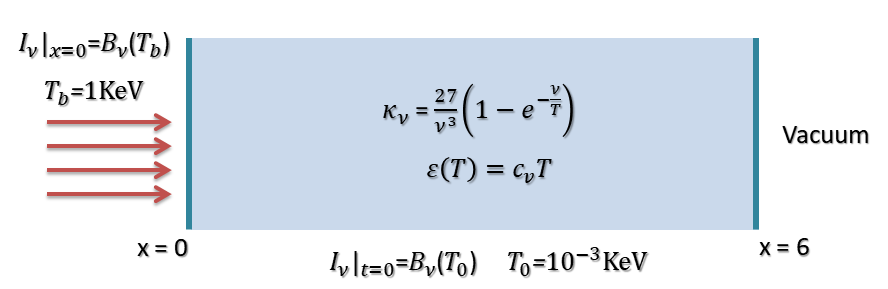
\includegraphics[width=0.75\textwidth]{FC_Test_1d.png}
		\caption{\label{fig:FC_Test_1d}
			Fleck and Cummings test problem}
	\end{figure}

	A 1D homogeneous slab is defined as 6 cm thick whose material opacity is given by
	\begin{equation}
		\varkappa_{\nu} = \frac{27}{\pr{h\nu}^3}\pr{1-e^{-\frac{h\nu}{kT}}}.
	\end{equation}
	
	The left boundary is subject to incoming radiation with black-body spectrum at temperature $T_b = 1$ keV and the right boundary is vacuum. The initial temperature of the slab is $T_0 =1$ eV, and the initial radiation distribution is given as the black-body spectrum at this temperature. This test approximates material energy density as a linear function of temperature
	\begin{equation}
		\varepsilon = \cv T,
	\end{equation}
	
	where the heat capacity of the material is given as
	\begin{equation}
		\cv = 0.5917\ar T_b^3.
	\end{equation}
	
	We use a uniform spatial mesh of 60 cells of length 0.1 cm, 17 energy groups and the double $S_4$ Gauss-Legendre quadrature set. Convergence criteria for temperature and energy density are $\epsilon_T=\epsilon_E=10^{-12}$. Fig. \ref{fig:ref_sols} displays the solution for temperature and total energy density for select instants of time obtained with the TRT problem by means of the MLQD method. Figure \ref{fig:ref_errs_inf_roms} presents the relative error of the solution of the $P_1$, $P_{\frac{1}{3}}$ and diffusion models to the MLQD solution in the $L_1$ norm. These models produce high errors at the early times of the problem and level off to a lower error once the steady state has been reached.
	
	%=================================================================================
	% TEST PROBLEM SOLUTIONS
	\begin{figure}[ht!]
		\centering
		\subfloat[Temperature \label{subfig:refcase_temp_sol}]{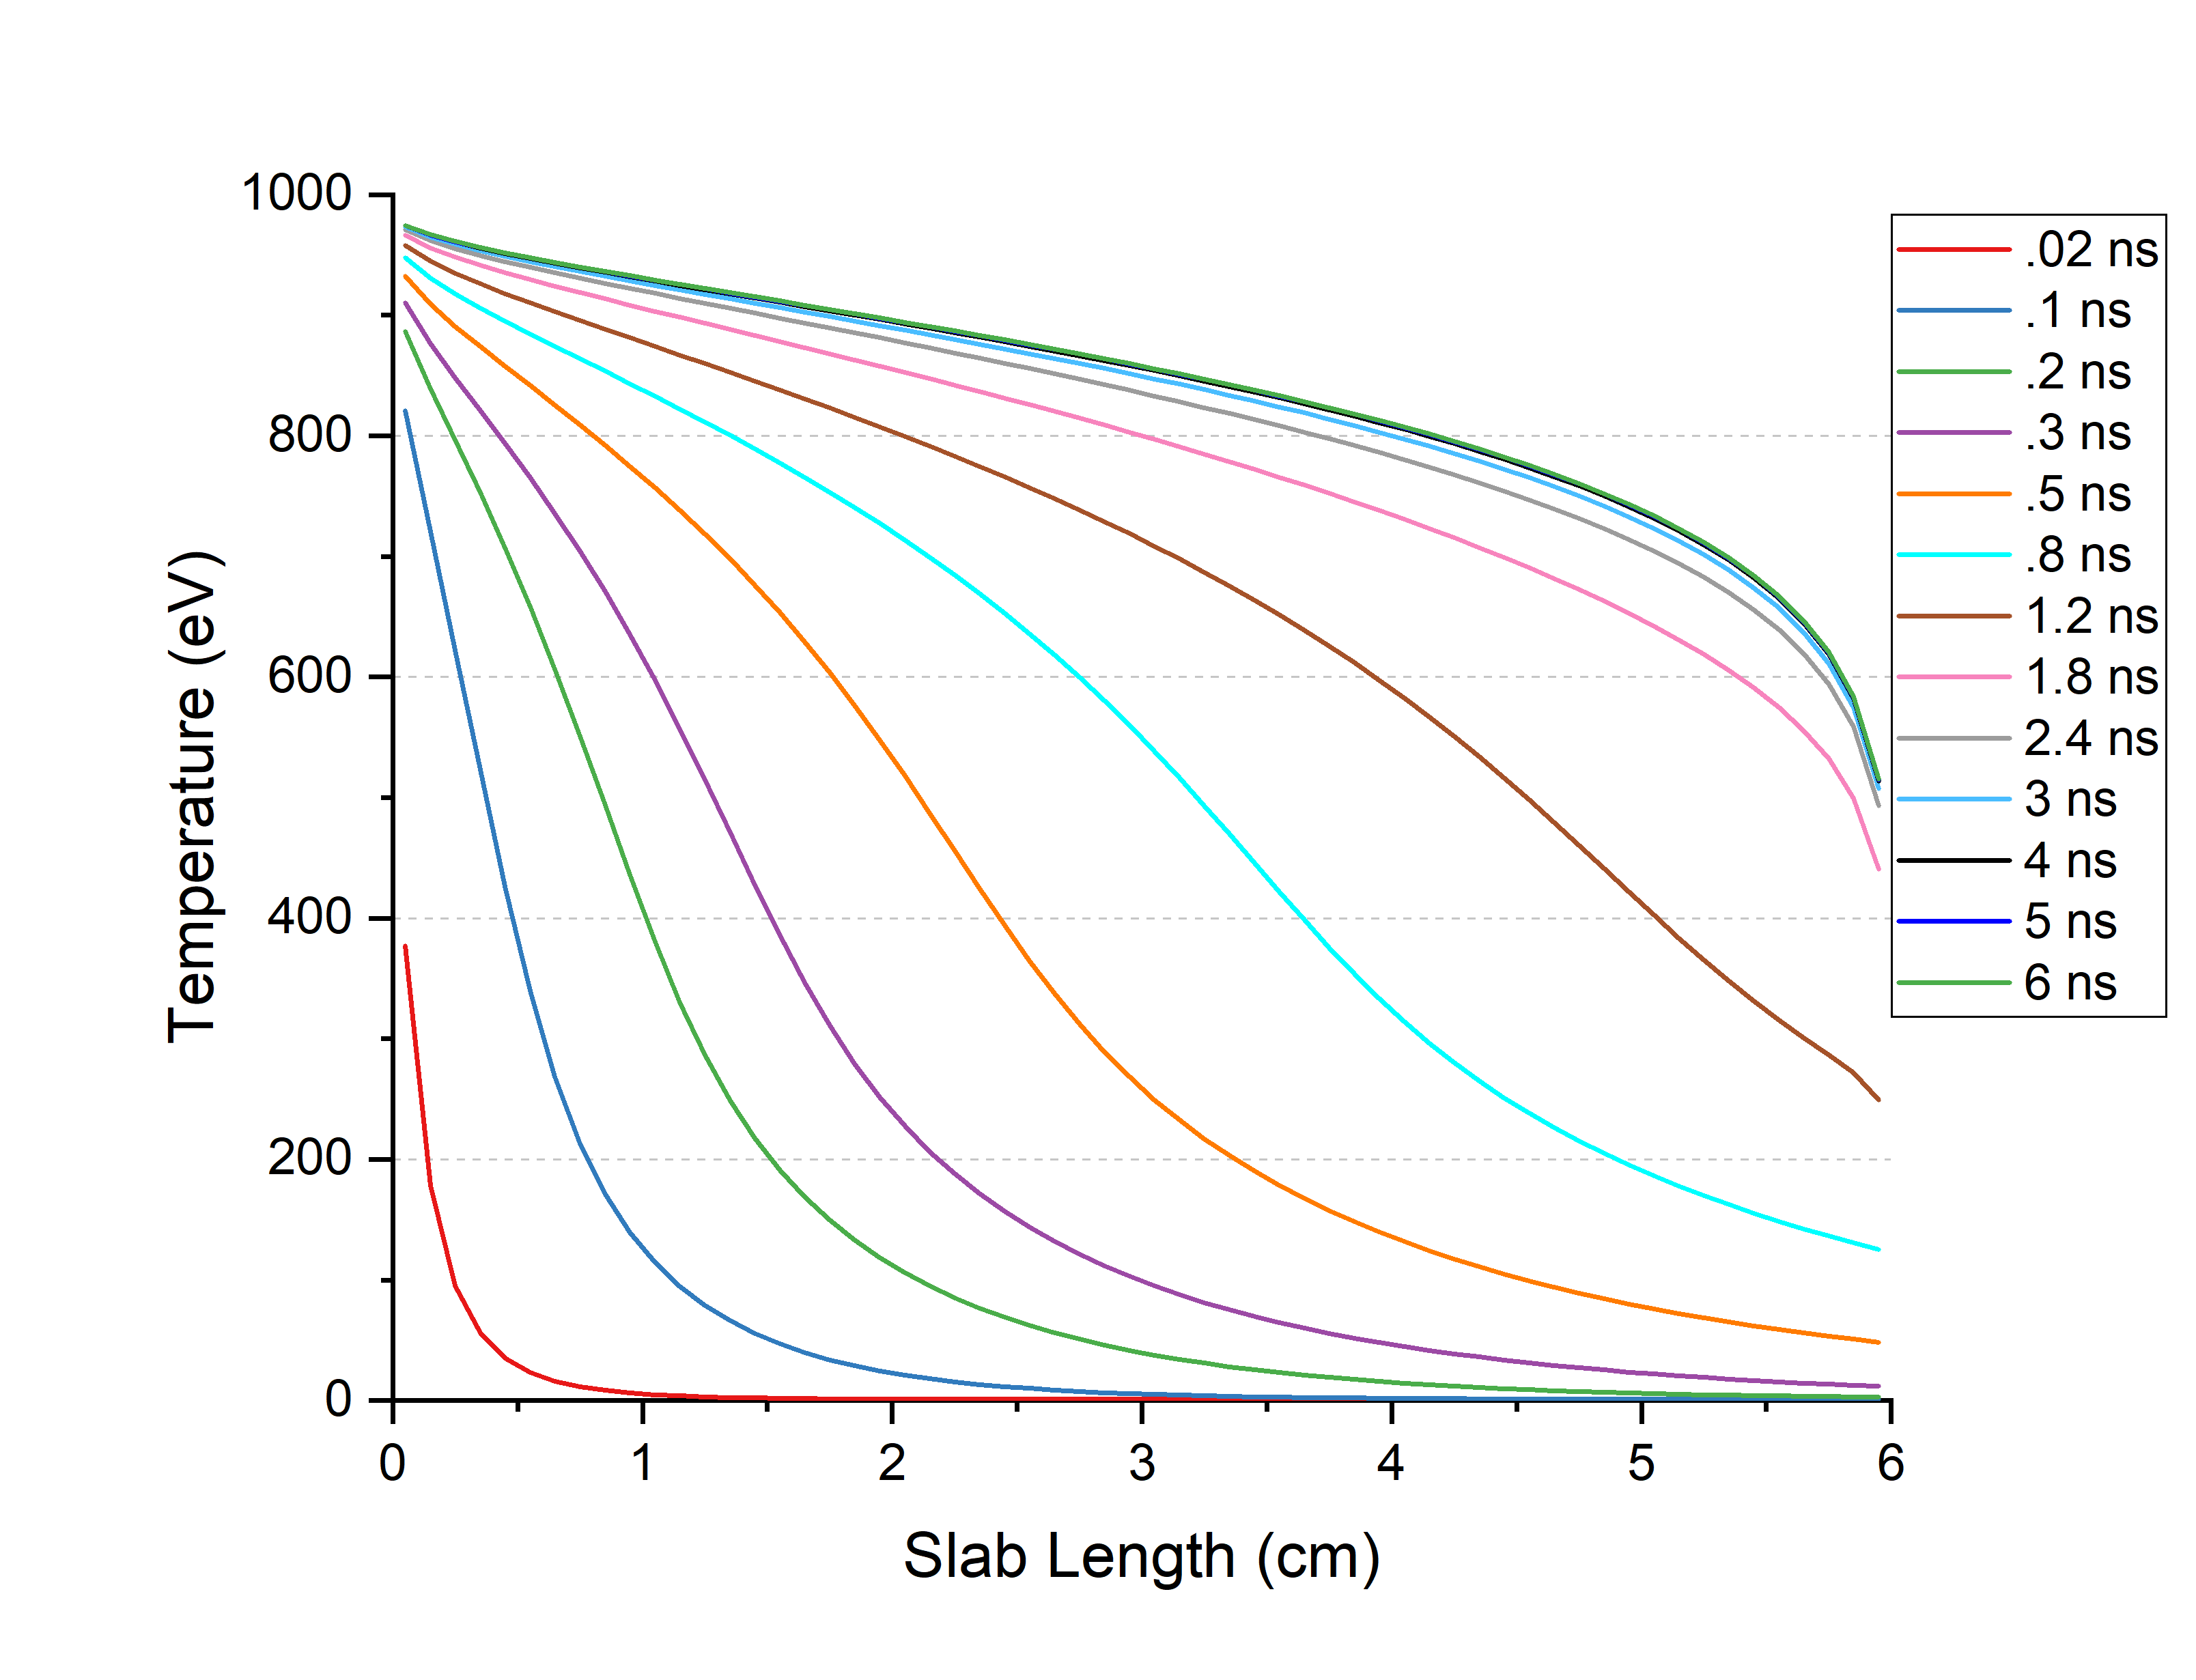
\includegraphics[width=0.5\textwidth]{refcase_temp_sol.png}}
		\subfloat[Total energy density \label{subfig:refcase_E_sol}]{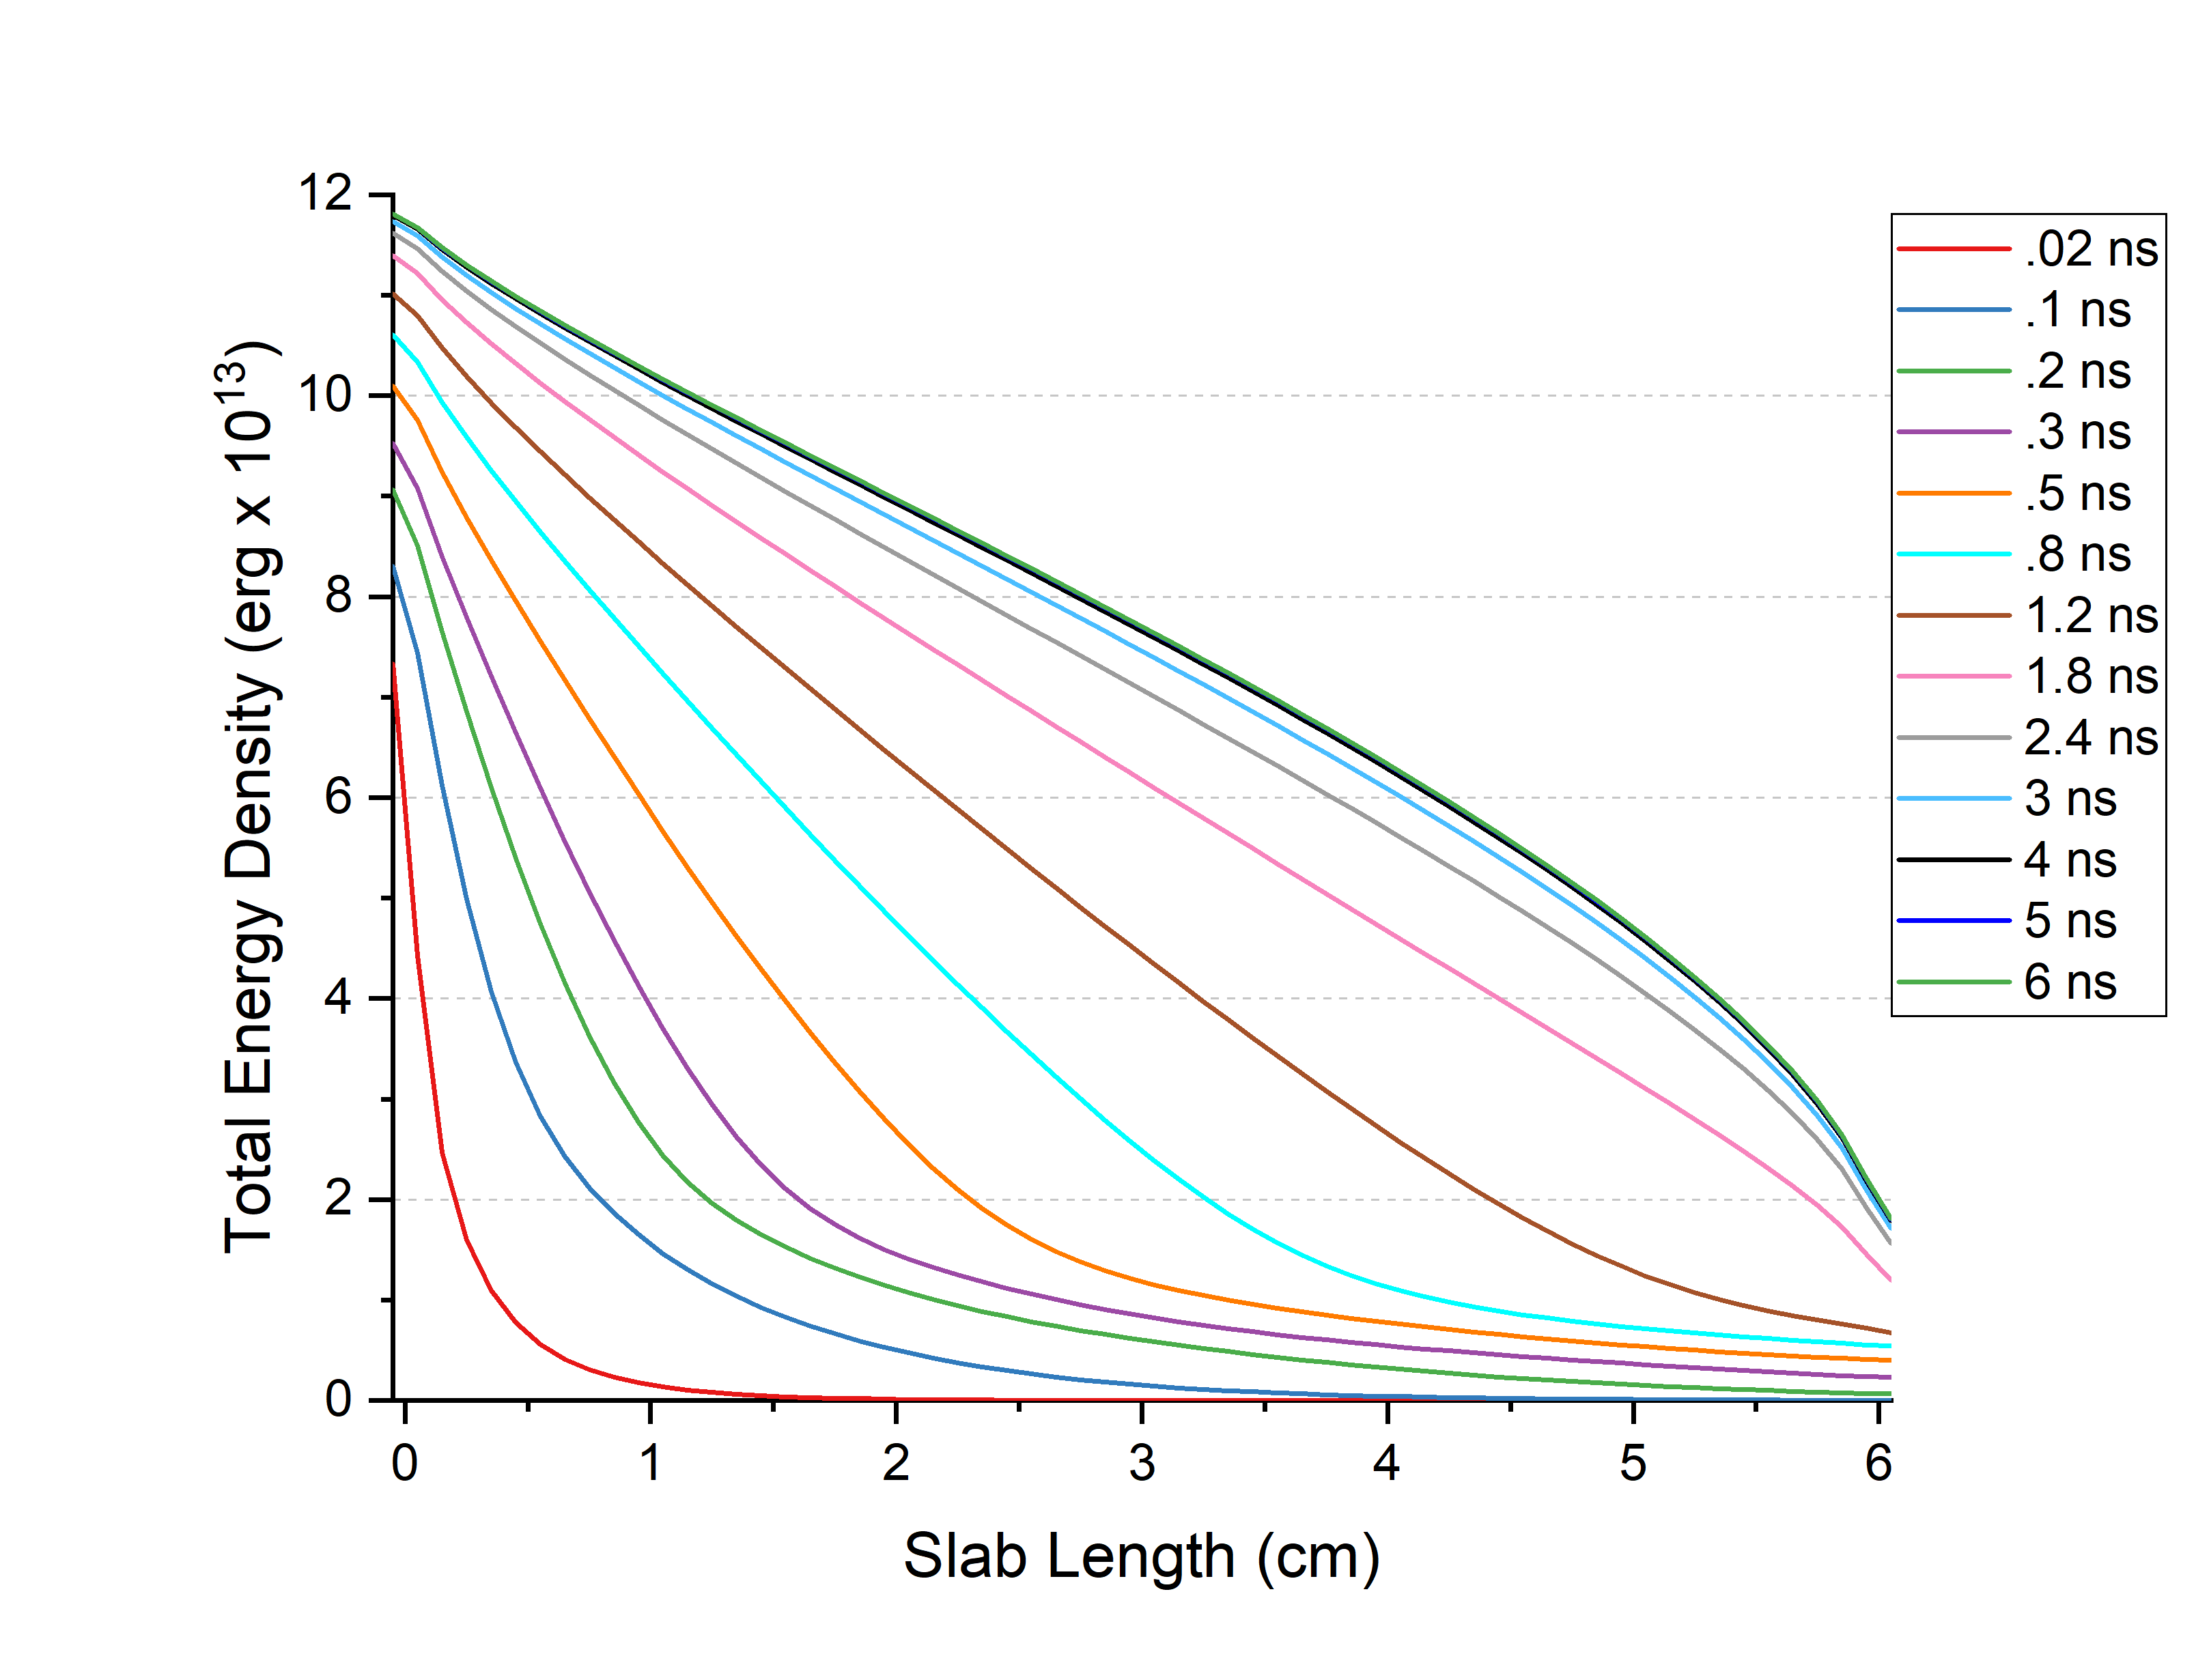
\includegraphics[width=0.5\textwidth]{refcase_E_sol.png}}
		\caption{\label{fig:ref_sols}
			RT solution obtained by the MLQD method to the F-C test problem.}
	\end{figure}

	%=================================================================================
	% TEST PROBLEM ERRORS
	\begin{figure}[ht!]
		\centering
		\subfloat[Temperature relative error \label{subfig:refcase_Temp_rel_inf_roms}]{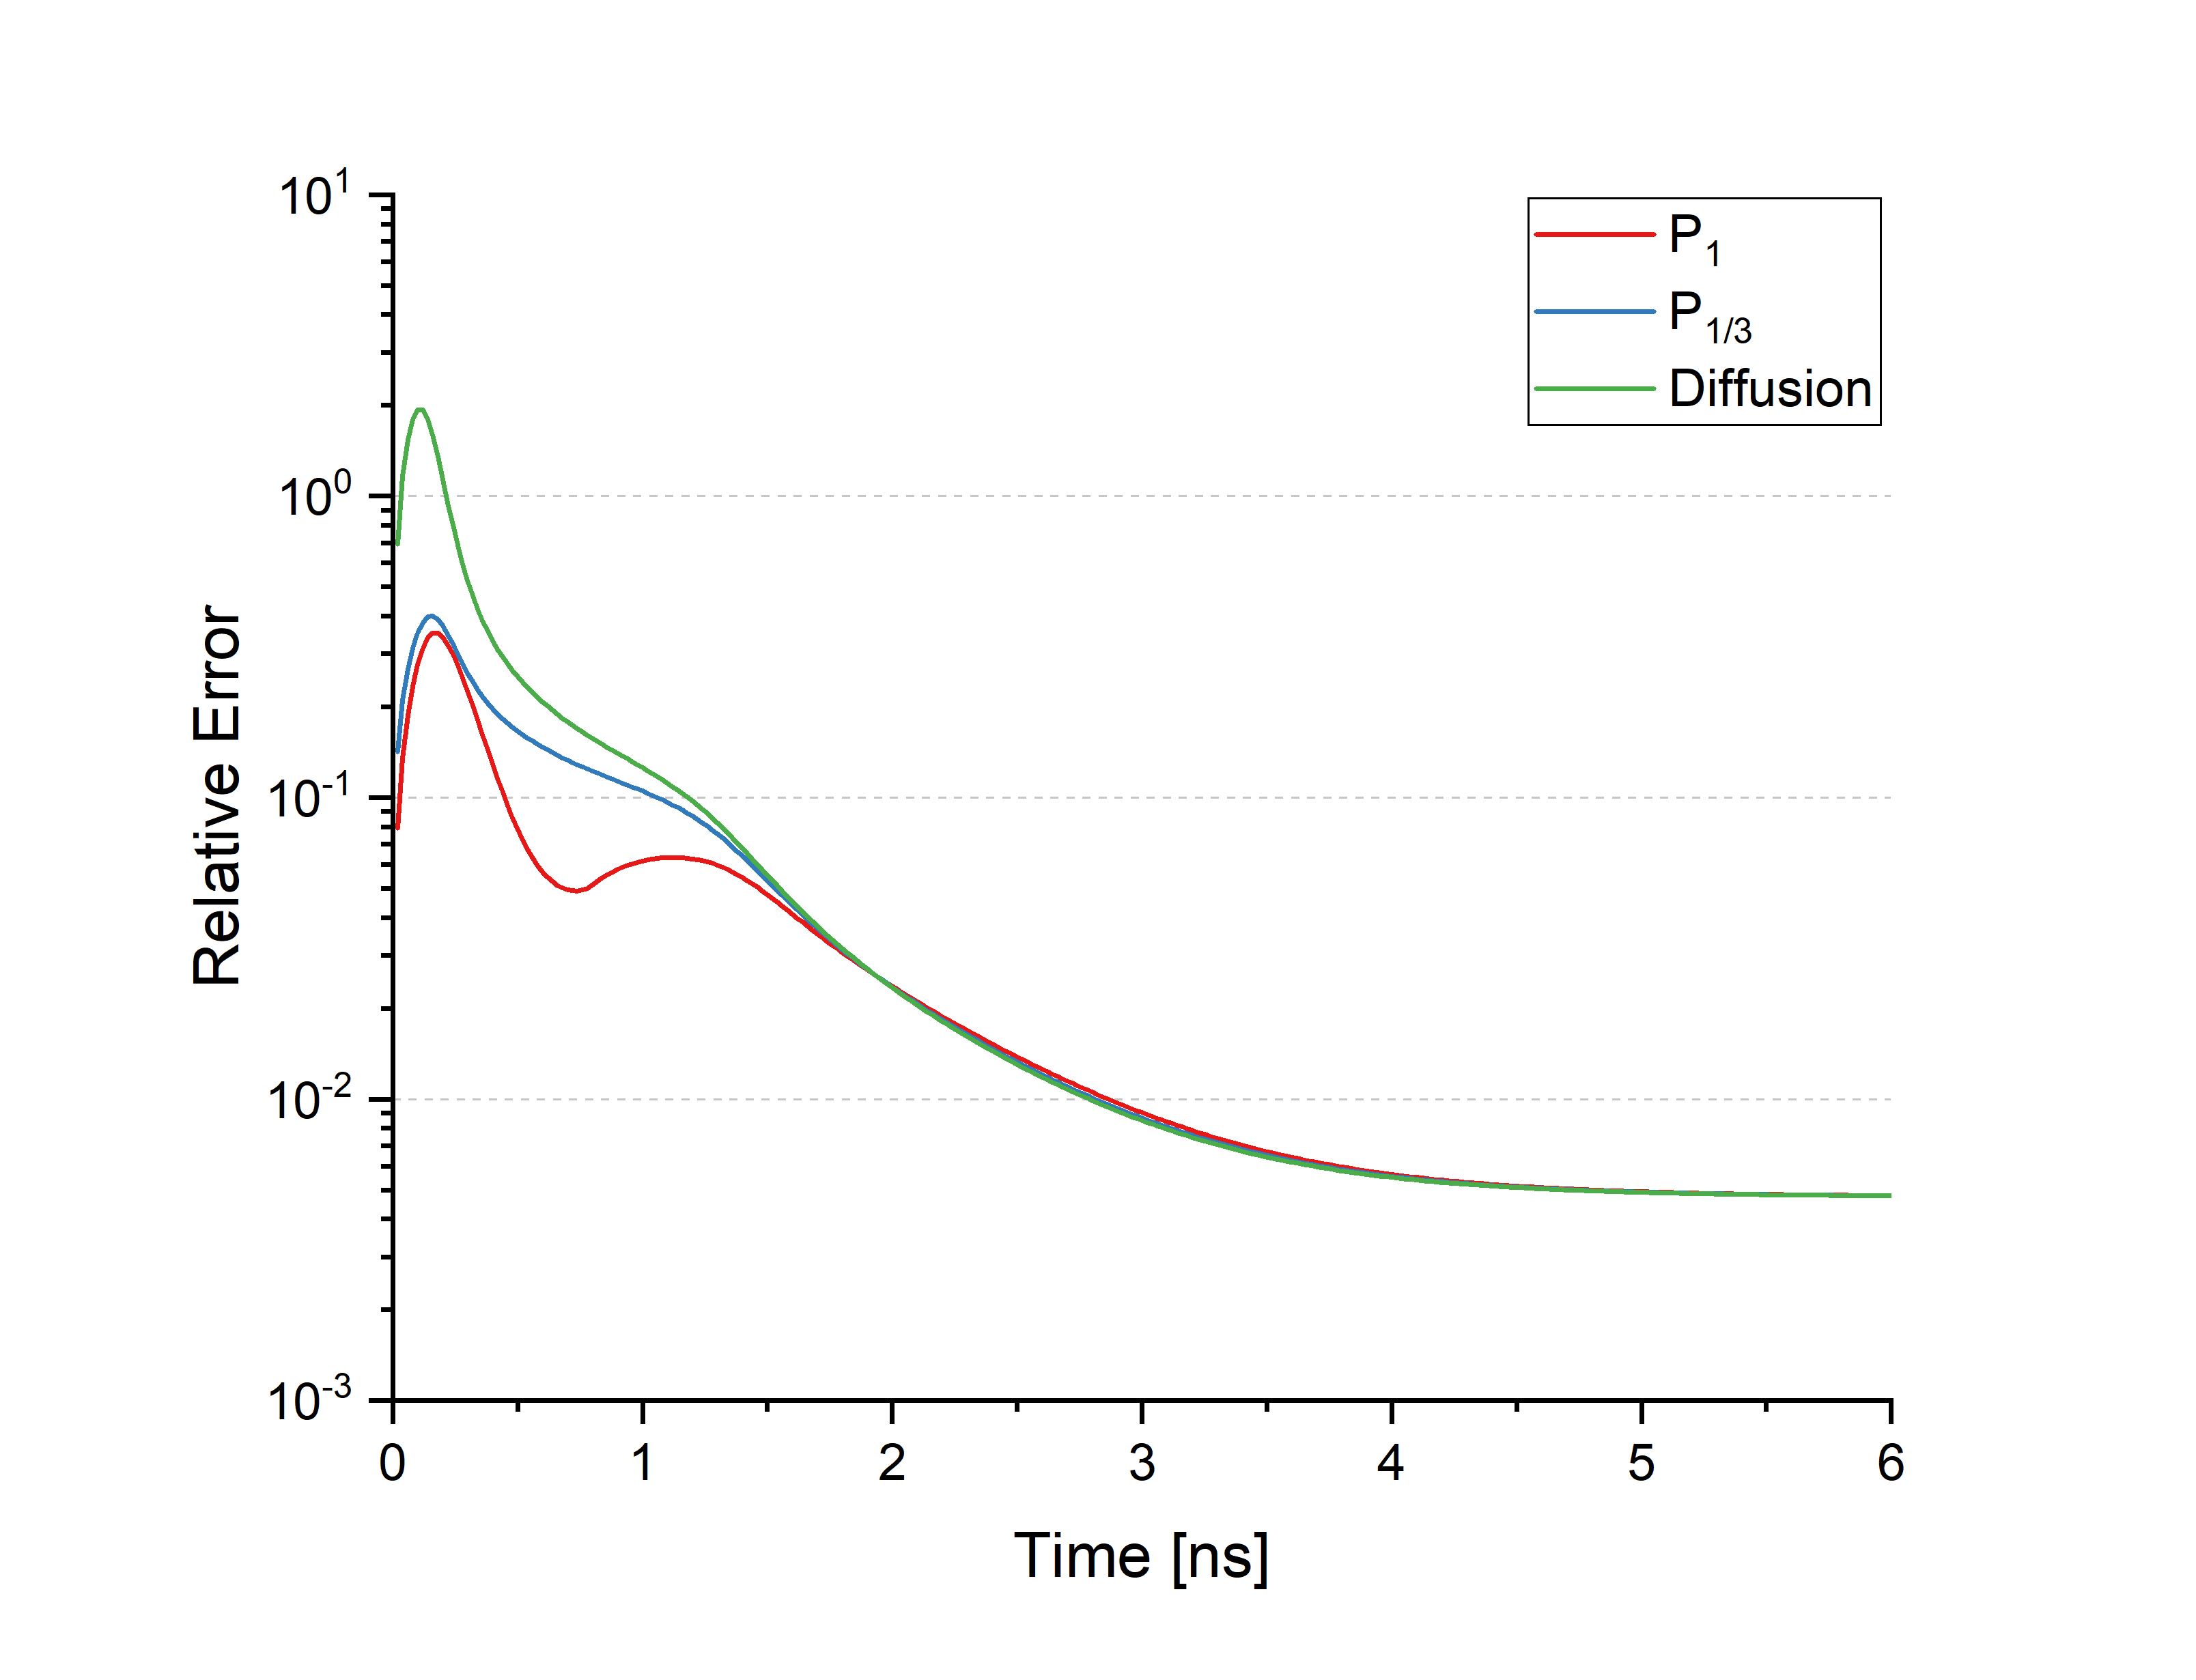
\includegraphics[width=0.5\textwidth]{refcase_Temp_rel_inf_roms.png}}
		\subfloat[Total energy density relative error \label{subfig:refcase_E_rel_inf_roms}]{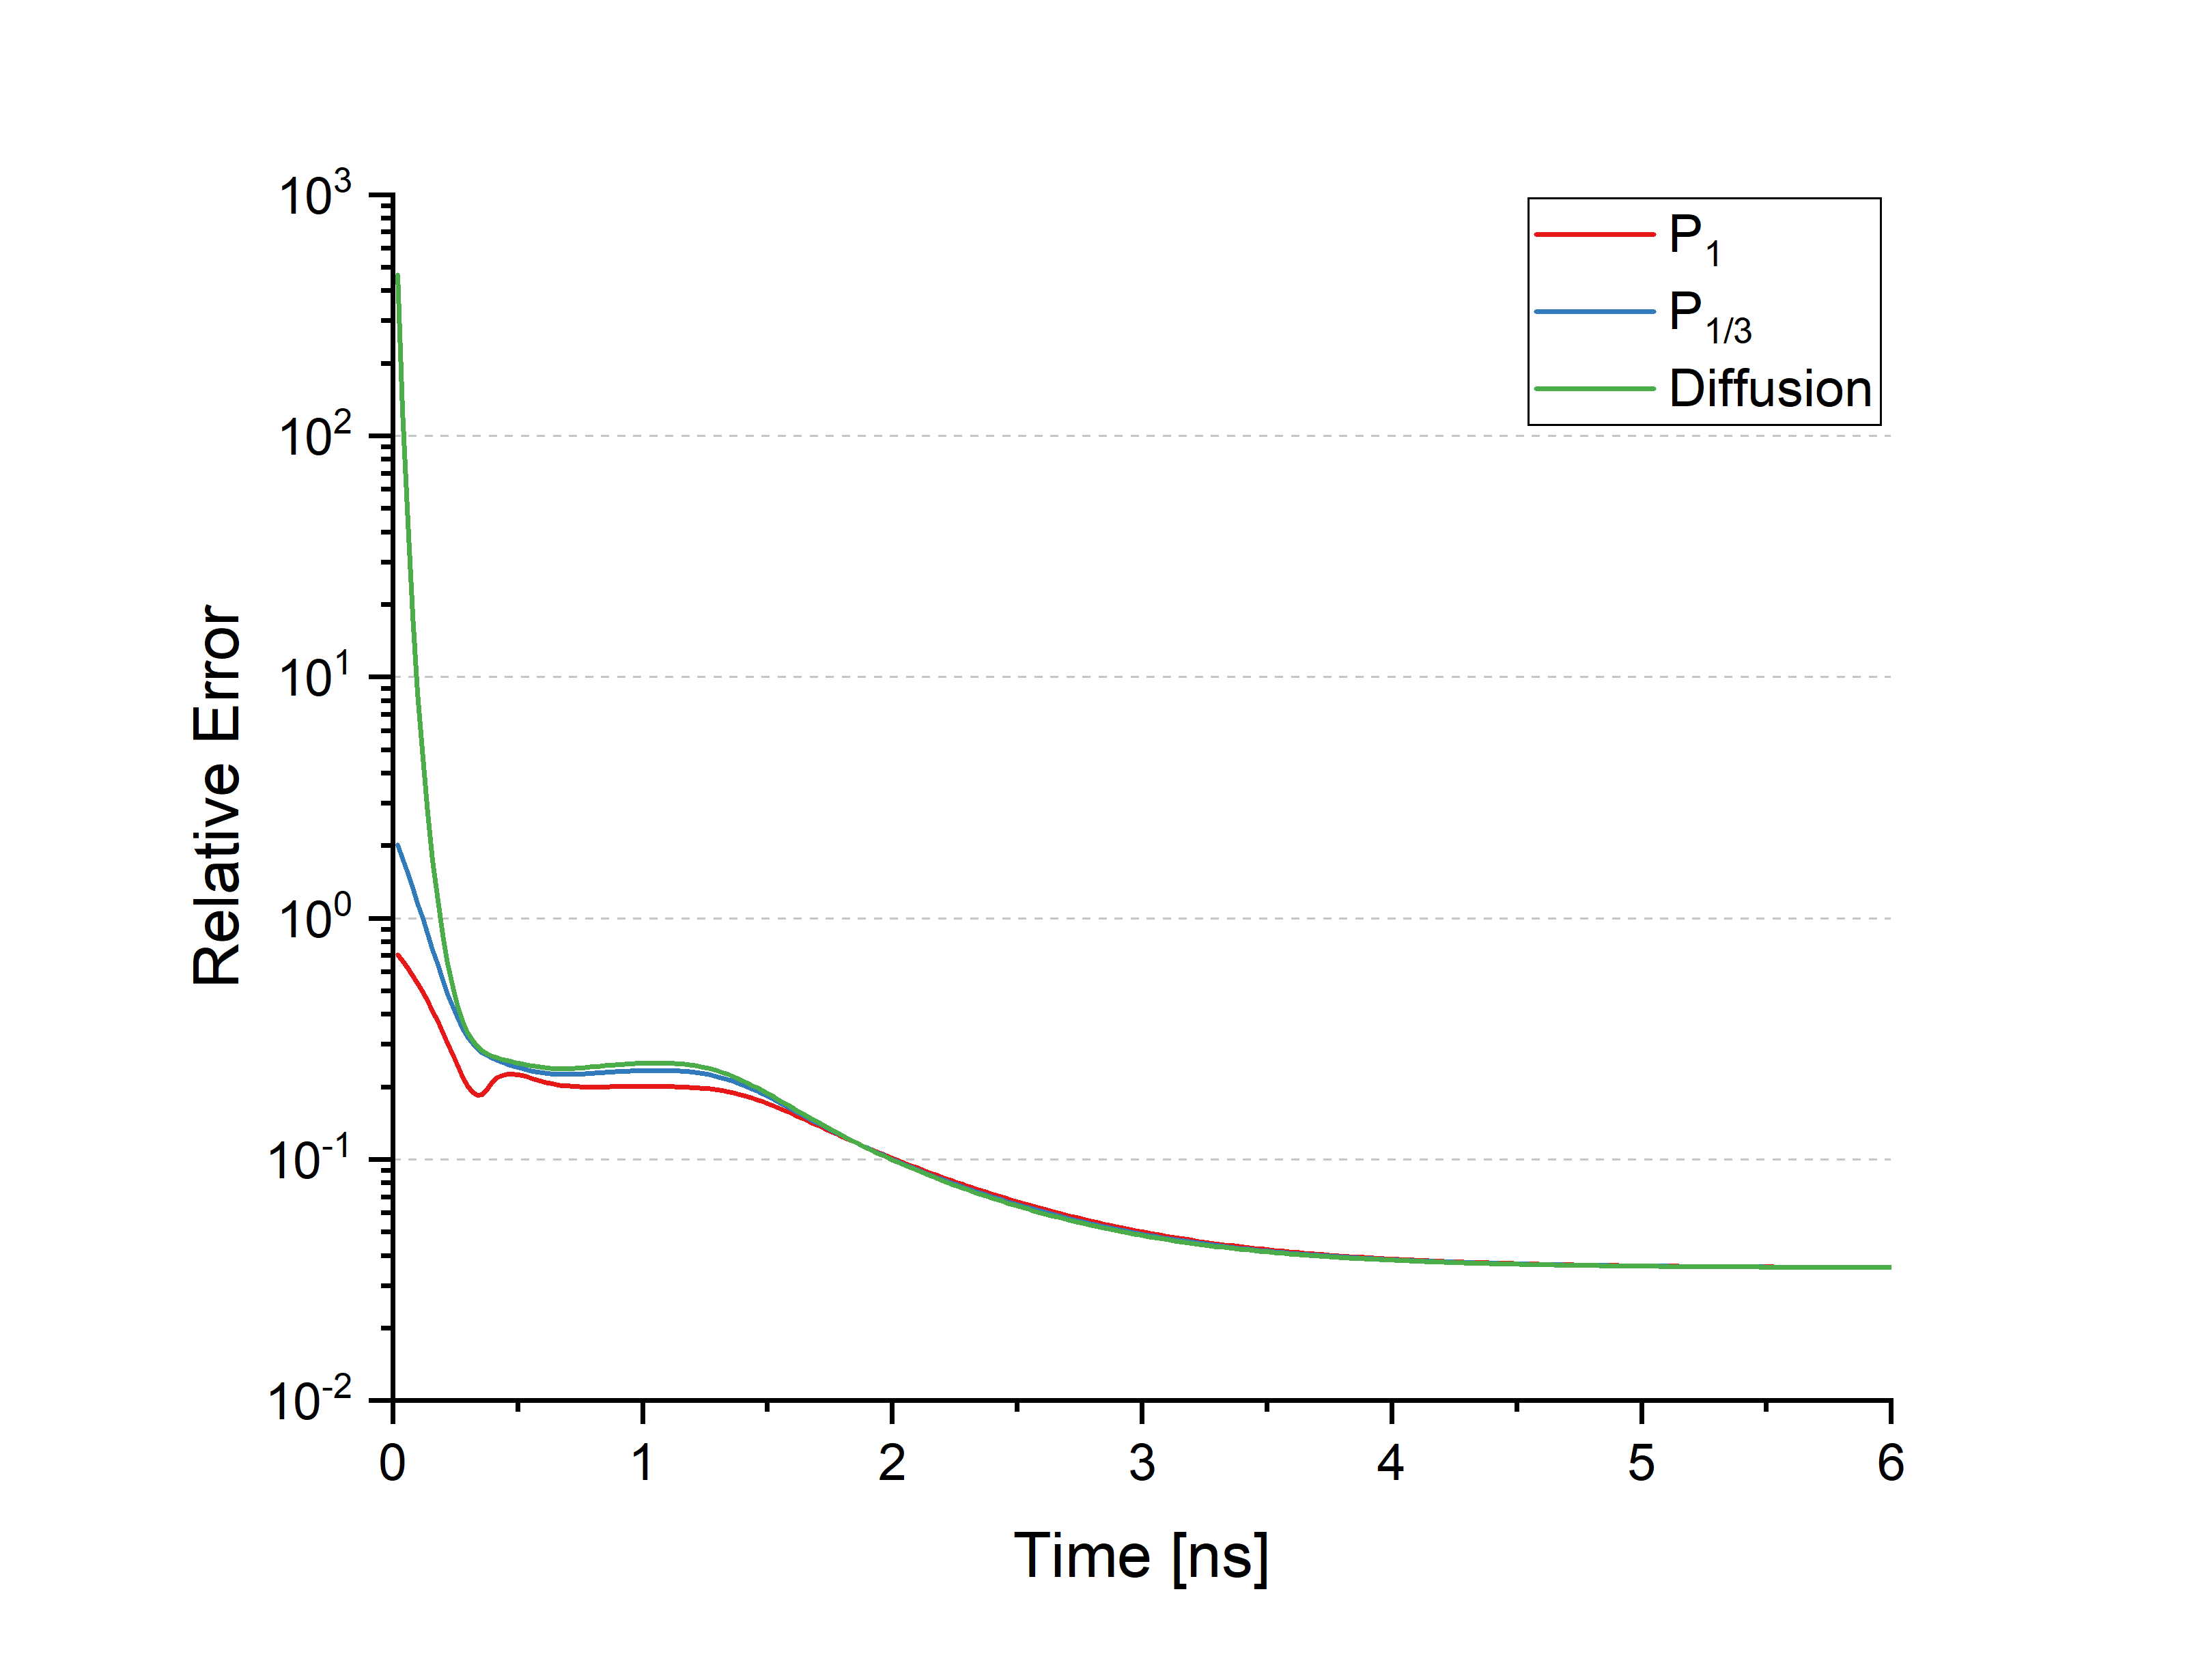
\includegraphics[width=0.5\textwidth]{refcase_E_rel_inf_roms.png}}
		\caption{\label{fig:ref_errs_inf_roms}
			Relative error of the $P_1$, $P_{\frac{1}{3}}$ \& Diffusion solution to the F-C test problem relative to the MLQD solution in $L_1$ norm}
	\end{figure}

\section{Low-Rank Approximation of Group QD Factors} \label{sec:reduced_qdf}
	%The first step in developing the MLOQD-POD ROM is to form a database of known group QD factors $\bA^f_g$. Given the solution to the F-C test problem, the reference group QD factors as a part of the solution of this TRT problem are known on some grid in phase space and time. The reference group QD factors are formed into $N_g$ matrices $\bA^f_g$ whose columns are the group $g$ QD factor solutions for each time step in chronological order. The truncated SVD of $\bA^f_g$ generates reduced rank approximations of the QD factors $\bA^{f*}_g$. 
	
	Fig. \ref{fig:QD_sval_summary} displays the normalized magnitudes and $1-\gamma_n$ \eqref{worth_gam} of the singular values of $\bA^f_g$ for different energy groups. Table \ref{tab:mqd_sigtab} displays the rank of approximation $(r_g)$ involved per energy group at different values of  $\varepsilon_\sigma$ \eqref{cutoff_eps}.
	
	\ind Since the test problem has 60 spatial cells the vector of cell-average QD factors in space has 62 values including 2 boundary values. When $\varepsilon_\sigma=10^{-12}$, the full-rank SVD is used. Note that group 2 uses a significantly higher rank SVD than any other energy group for large $\varepsilon_\sigma$.  This behavior can be explained with Fig. \ref{subfig:QD_svals}, which depicts the singular values normalized to the largest singular value for 7 sample energy groups $\pr{g=1,2,3,4,8,12,17}$. Group 2 is the only group to have two plateau regions, of which the first is high in value. This leads to high-order expansions in group 2 for even large $\varepsilon_\sigma$. The point where the singular values level off to a lower bound is smaller for each successive energy group excluding group 1.
	
	\ind Fig. \ref{subfig:inv_worths} displays $1-\gamma_n$ for each energy group and value of $n$ to show $\gamma_n$ of each successive reduced rank approximation of the QD factors per energy group. $1-\gamma_n$ is chosen over $\gamma_n$ for sake of clarity as it is much easier to analyze on a plot. Some of the latter energy groups quickly reach a value of $10^{-16}$ or numerically zero fairly early, as soon as $n=30$. As seen in Fig. \ref{subfig:QD_svals}, group 2 forms a unique shape among the other curves and demonstrates that significantly higher rank must be used compared to other groups to decrease the value of $1-\gamma_n$.

 	%=================================================================================
 	% SINGULAR VALUE FIGS
	\begin{figure}[ht!]
		\centering
		\subfloat[Normalized singular values of $\bA^f_g$ (QD factor database matrices) \label{subfig:QD_svals}]{\includegraphics[width=0.5\textwidth]{QD_svals.png}}
		\subfloat[$1-\gamma_n$ for $\bA^f_g$ (QD factor database matrices) \label{subfig:inv_worths}]{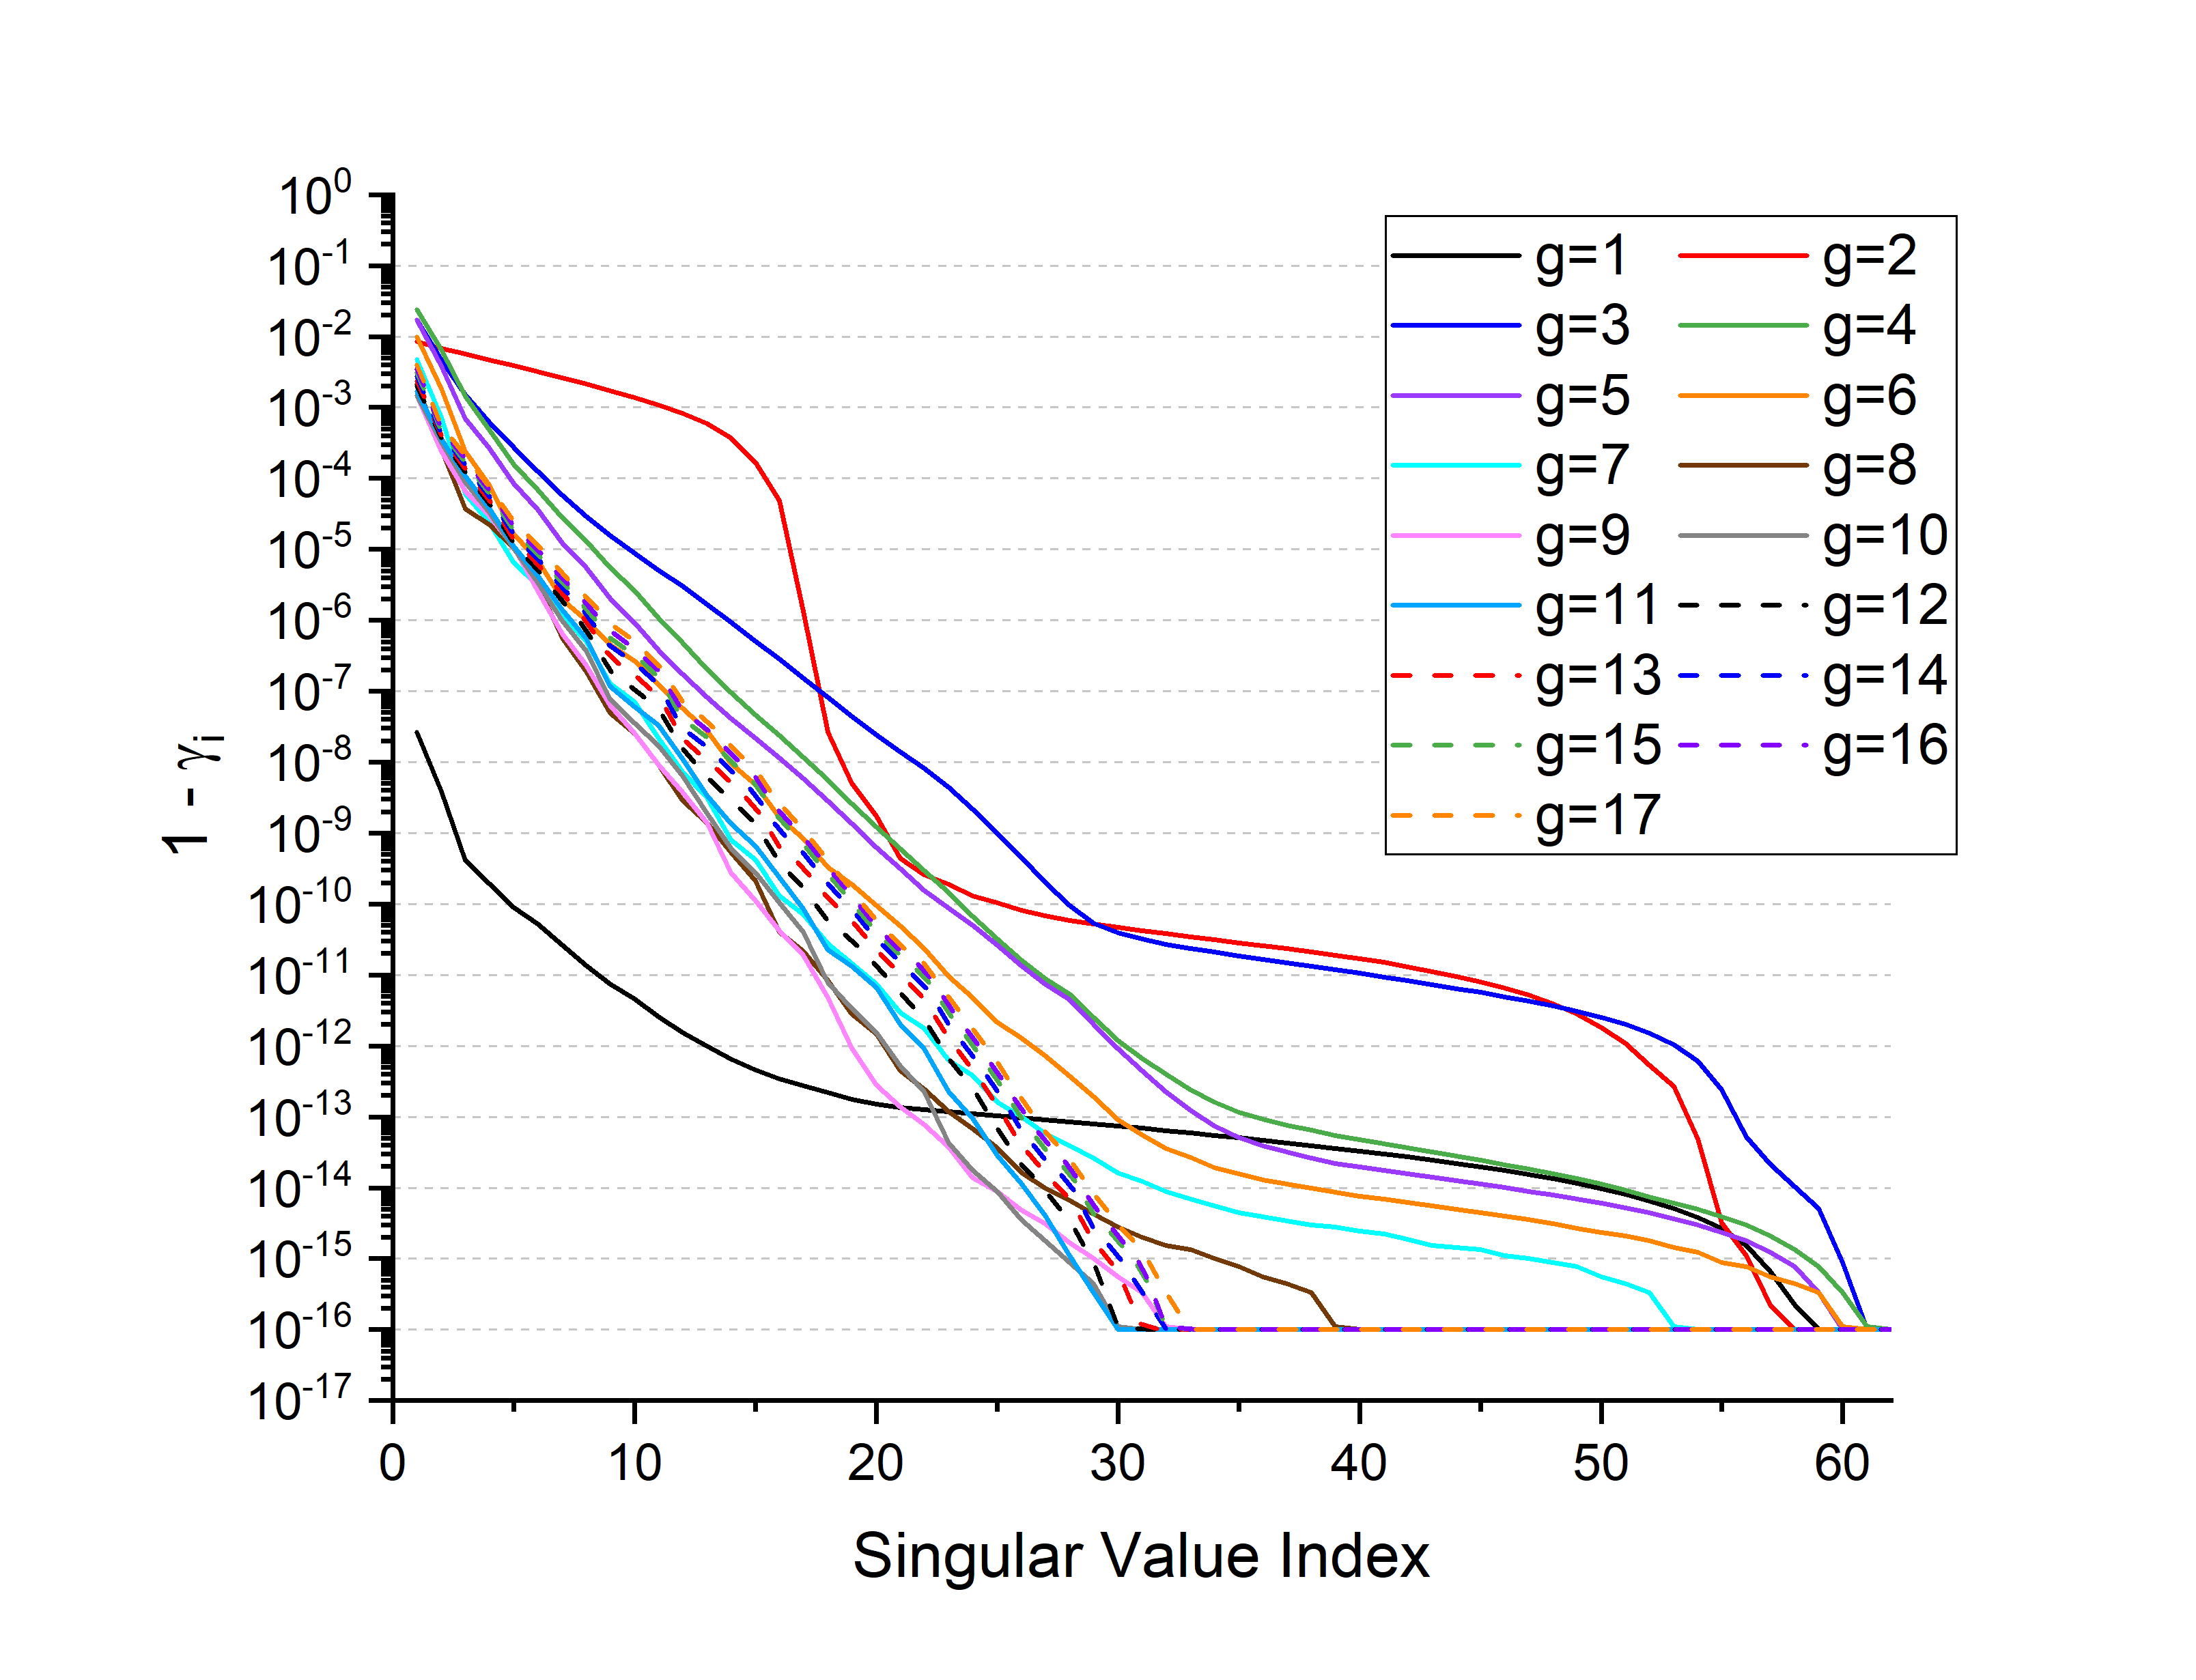
\includegraphics[width=0.5\textwidth]{inv_worths.png}}
		\caption{\label{fig:QD_sval_summary}
			Group QD factor normalized singular values and $1-\gamma_n$}
	\end{figure}
	
	%=================================================================================
	% SINGULAR VALUE TABLE
	\begin{table}[ht!]
		\caption{	\label{tab:mqd_sigtab} The rank of approximation $(r_g)$ of $f_g$ in each energy group for decreasing values of $\varepsilon_\sigma$}
		\begin{tabular}{|c||c|c|c|c|c|c|c|c|c|c|c|c|c|c|c|c|c|}	
			\hline
			$\varepsilon_\sigma \backslash  \ g$ & 1 & 2 & 3 & 4 & 5 & 6 & 7 & 8 & 9 & 10 & 11 & 12 & 13 & 14 & 15 & 16 & 17 \\
			\hline
			\hline
			$10^{-1}$ & 1  &  1 & 2  & 2  & 2  & 1  &  1 & 1 &  1 &   1 & 1 &  1 &  1 & 1 &  1 &  1 & 1 \\ \hline
			$10^{-2}$ & 1 & 16 & 6 & 5 & 5 & 4 & 3 & 3 & 3 & 3 & 3 & 3 & 3 & 4 & 4 & 4 & 4\\ \hline
			$10^{-3}$ & 1 & 18 & 13 & 11 & 10 & 7 & 7 & 7 & 7 & 7 & 7 & 8 & 8 & 8 & 8 & 9 & 9\\ \hline
			$10^{-4}$ & 2 & 19 & 21 & 17 & 16 & 14 & 12 & 11 & 11 & 12 & 12 & 12 & 13 & 13 & 14 & 14 & 14\\ \hline
			$10^{-12}$ & 62 & 62 & 62 & 62 & 62 & 62 & 62 & 62 & 62 & 62 & 62 & 62 & 62 & 62 & 62 & 62 & 62\\ \hline
		\end{tabular}
	\end{table}

	
	\ind To investigate the causes for the results shown in Fig. \ref{fig:QD_sval_summary} and Table \ref{tab:mqd_sigtab} we observe the actual reduced rank forms of the QD factors. Select energy groups $g=\pr{2,3,8}$ are chosen as groups 2 and 3 require the highest ranks for large $\varepsilon_\sigma$, and group 8 is a good representative energy group for the rest of the group QD factors. Figs. \ref{fig:qdf_g2_recomps}, \ref{fig:qdf_g3_recomps} and \ref{fig:qdf_g8_recomps} show the low-rank approximations of the group QD factors $f_g^*$ for groups 2, 3 and 8 respectively. Each of these figures displays the approximate QD factors obtained for 6 different ranks $r=\pr{1,2,5,10,15,20}$. These figures show more clearly the reason for groups 2 and 3 being the most difficult to approximate with low rank. For all plots shown when r = 20 are used $\pr{r=20}$, the structure of the approximate QD factors has converged to the high order MLQD solution to the resolution of the plot.
	
	\ind For groups 2 and 3 the approximate QD factors are structured as a fast moving wave during the initial stage of the TRT problem that is related to the propagation of the radiation front in these energy groups that are optically thick at this stage. Group 8 shows a smoother wave structure because photons in this more optically thin group move faster through the spatial domain. The structure of the group 2 approximate QD factors is unique due to the discontinuous nature of the waves. They display a sharp drop at the end of each wave dropping to a value of 1/3. Since this must then be propagated from the left boundary to the right, an SVD of higher rank is required to recreate this structure with its sharp discontinuities. Thus Fig. \ref{fig:qdf_g2_recomps} shows the reduced rank forms of the group 2 approximate QD factors taking on a poor representation of the full rank form until at least $r=15$.
	
	\ind In Fig. \ref{fig:qdf_g3_recomps}, the group 3 approximate QD factors have converged to the resolution of the plot by the time the SVD with $r=15$ has been used, and most of the full rank form has been recreated with $r=10$. The group 8 approximate QD factors require an SVD of even smaller rank for the same accuracy, having converged to the full rank form by the resolution of the plot of Fig. \ref{fig:qdf_g8_recomps} for $r=10$. Using an SVD with $r=5$ for the approximate QD factors in group 8 also gives a very similar structure.

	%=================================================================================
	% QDF G2 RECOMP
	\begin{figure}[ht!]
		\centering
		\subfloat[r = 1 \label{subfig:qdf_g2_cut1}]{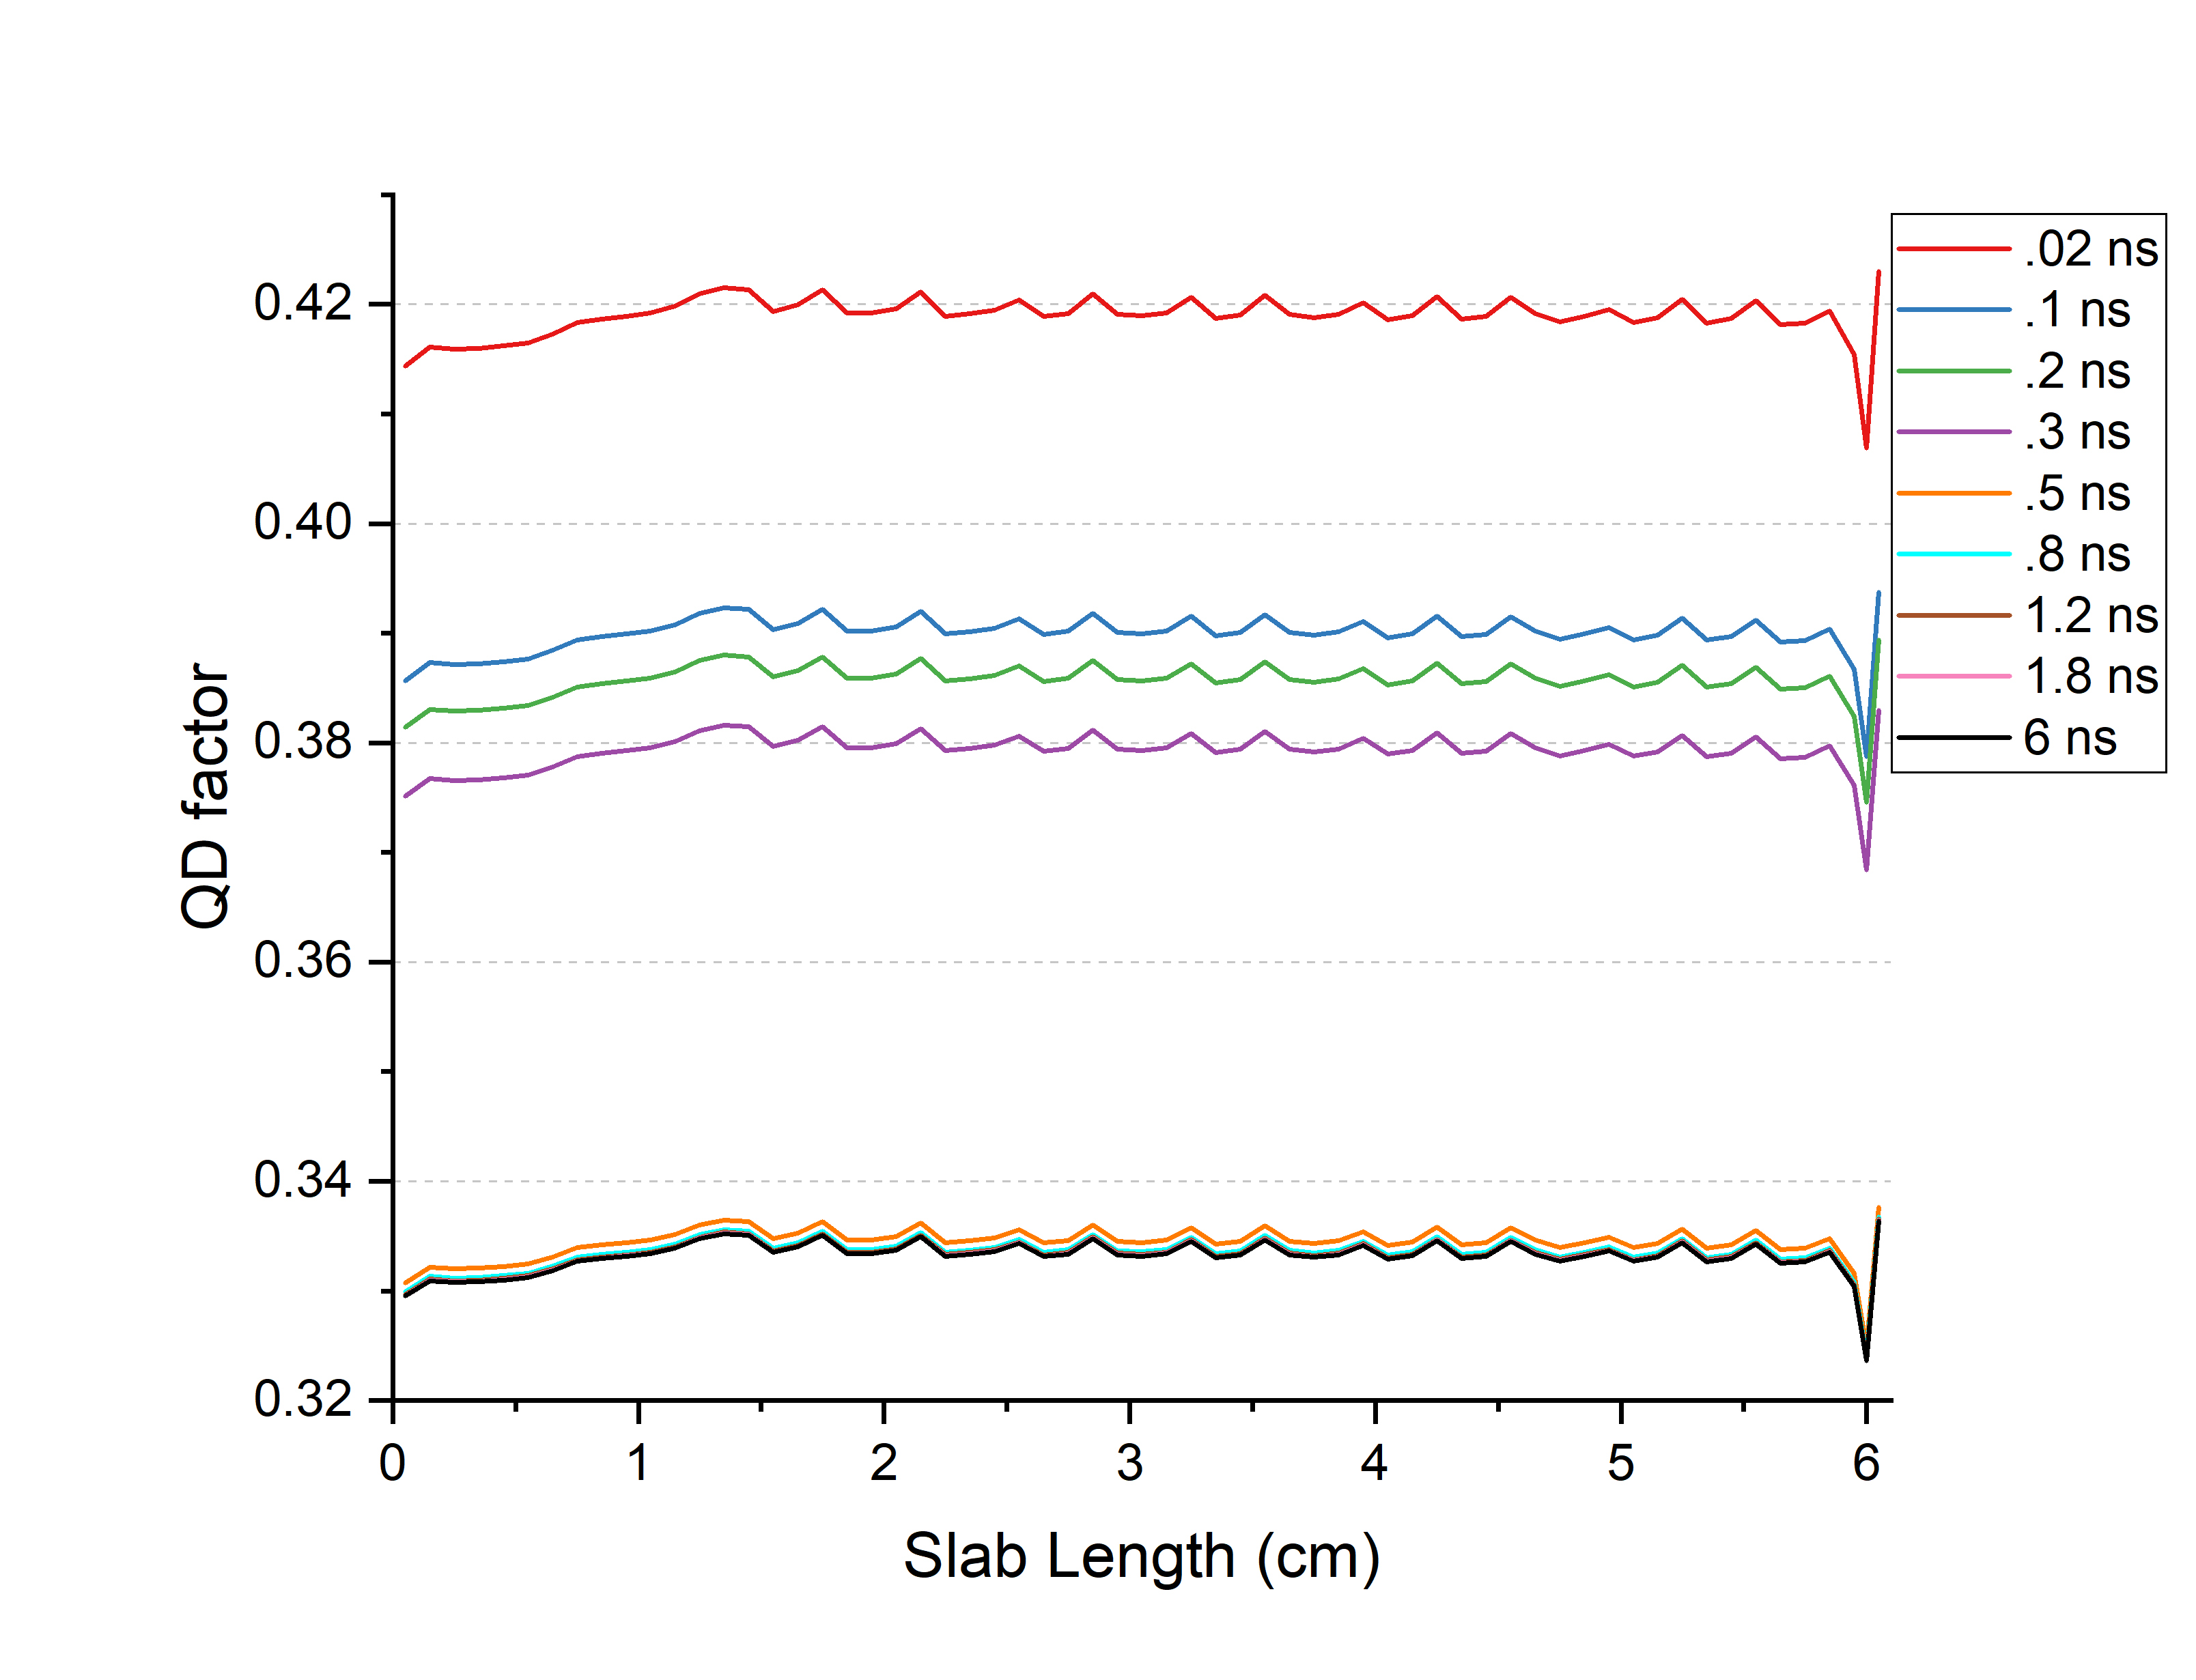
\includegraphics[width=0.5\textwidth]{qdf_g2_cut1.png}}
		\subfloat[r = 2 \label{subfig:qdf_g2_cut2}]{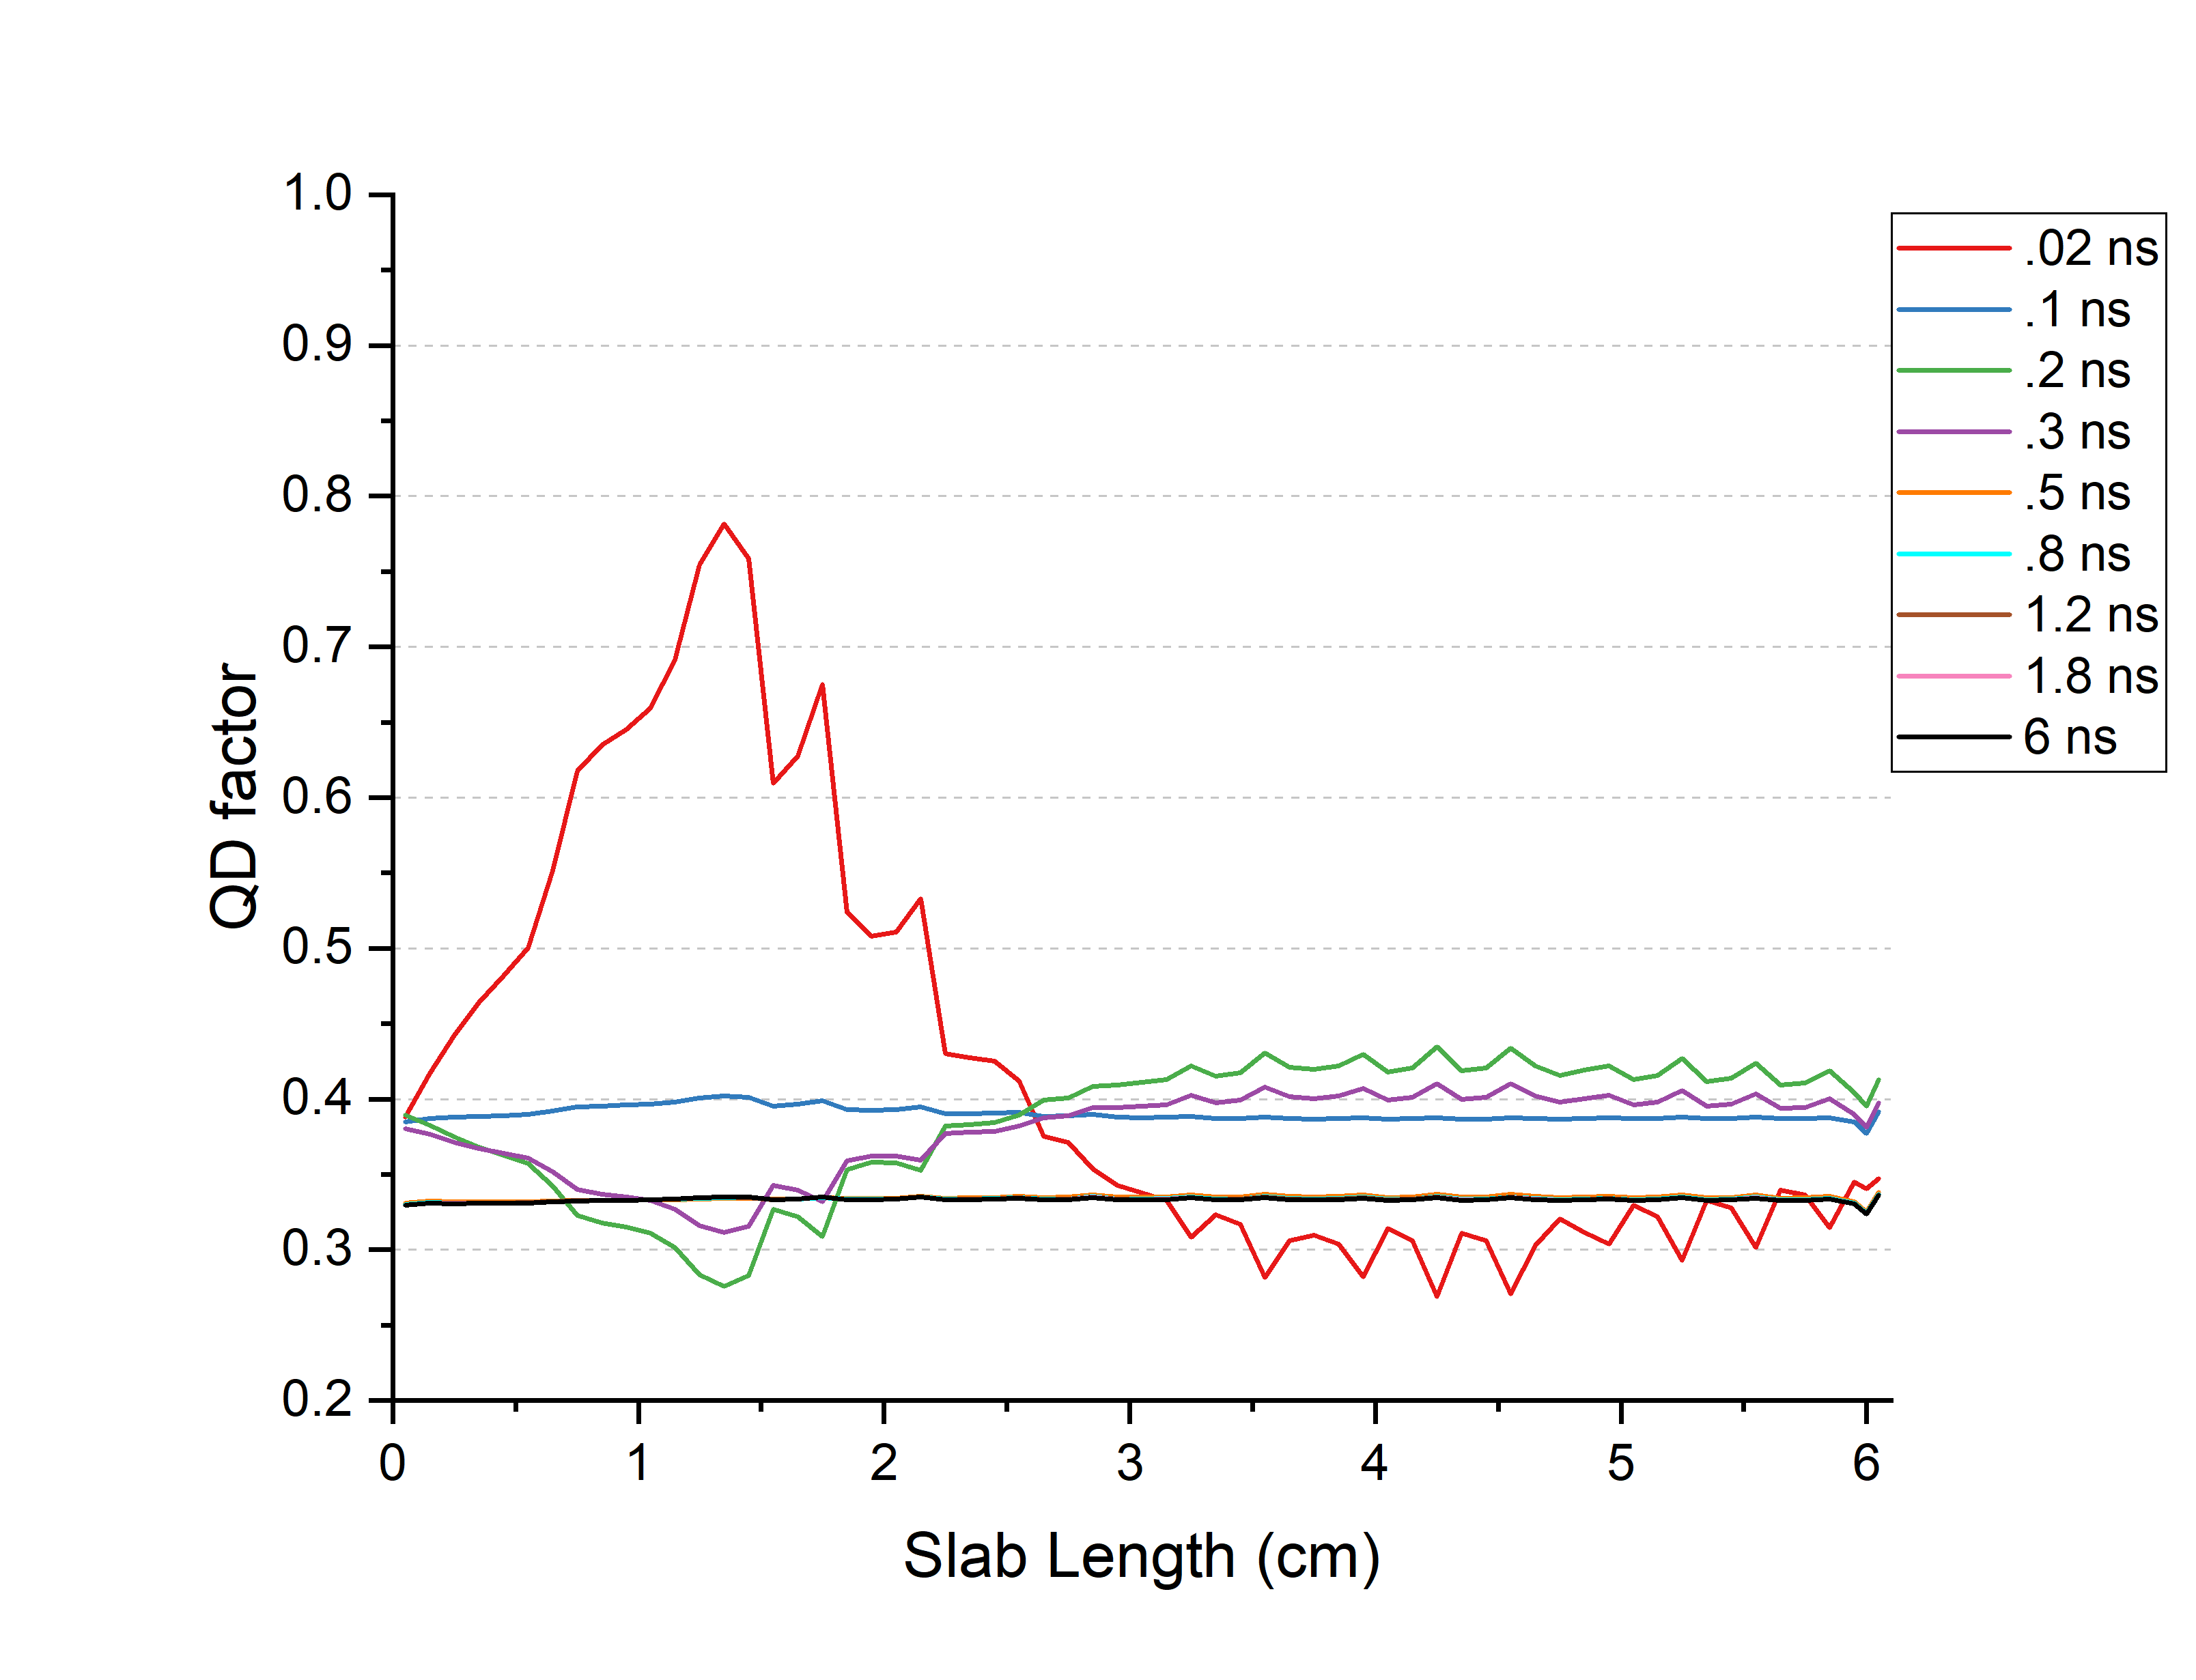
\includegraphics[width=0.5\textwidth]{qdf_g2_cut2.png}}\\
		\subfloat[r = 5 \label{subfig:qdf_g2_cut5}]{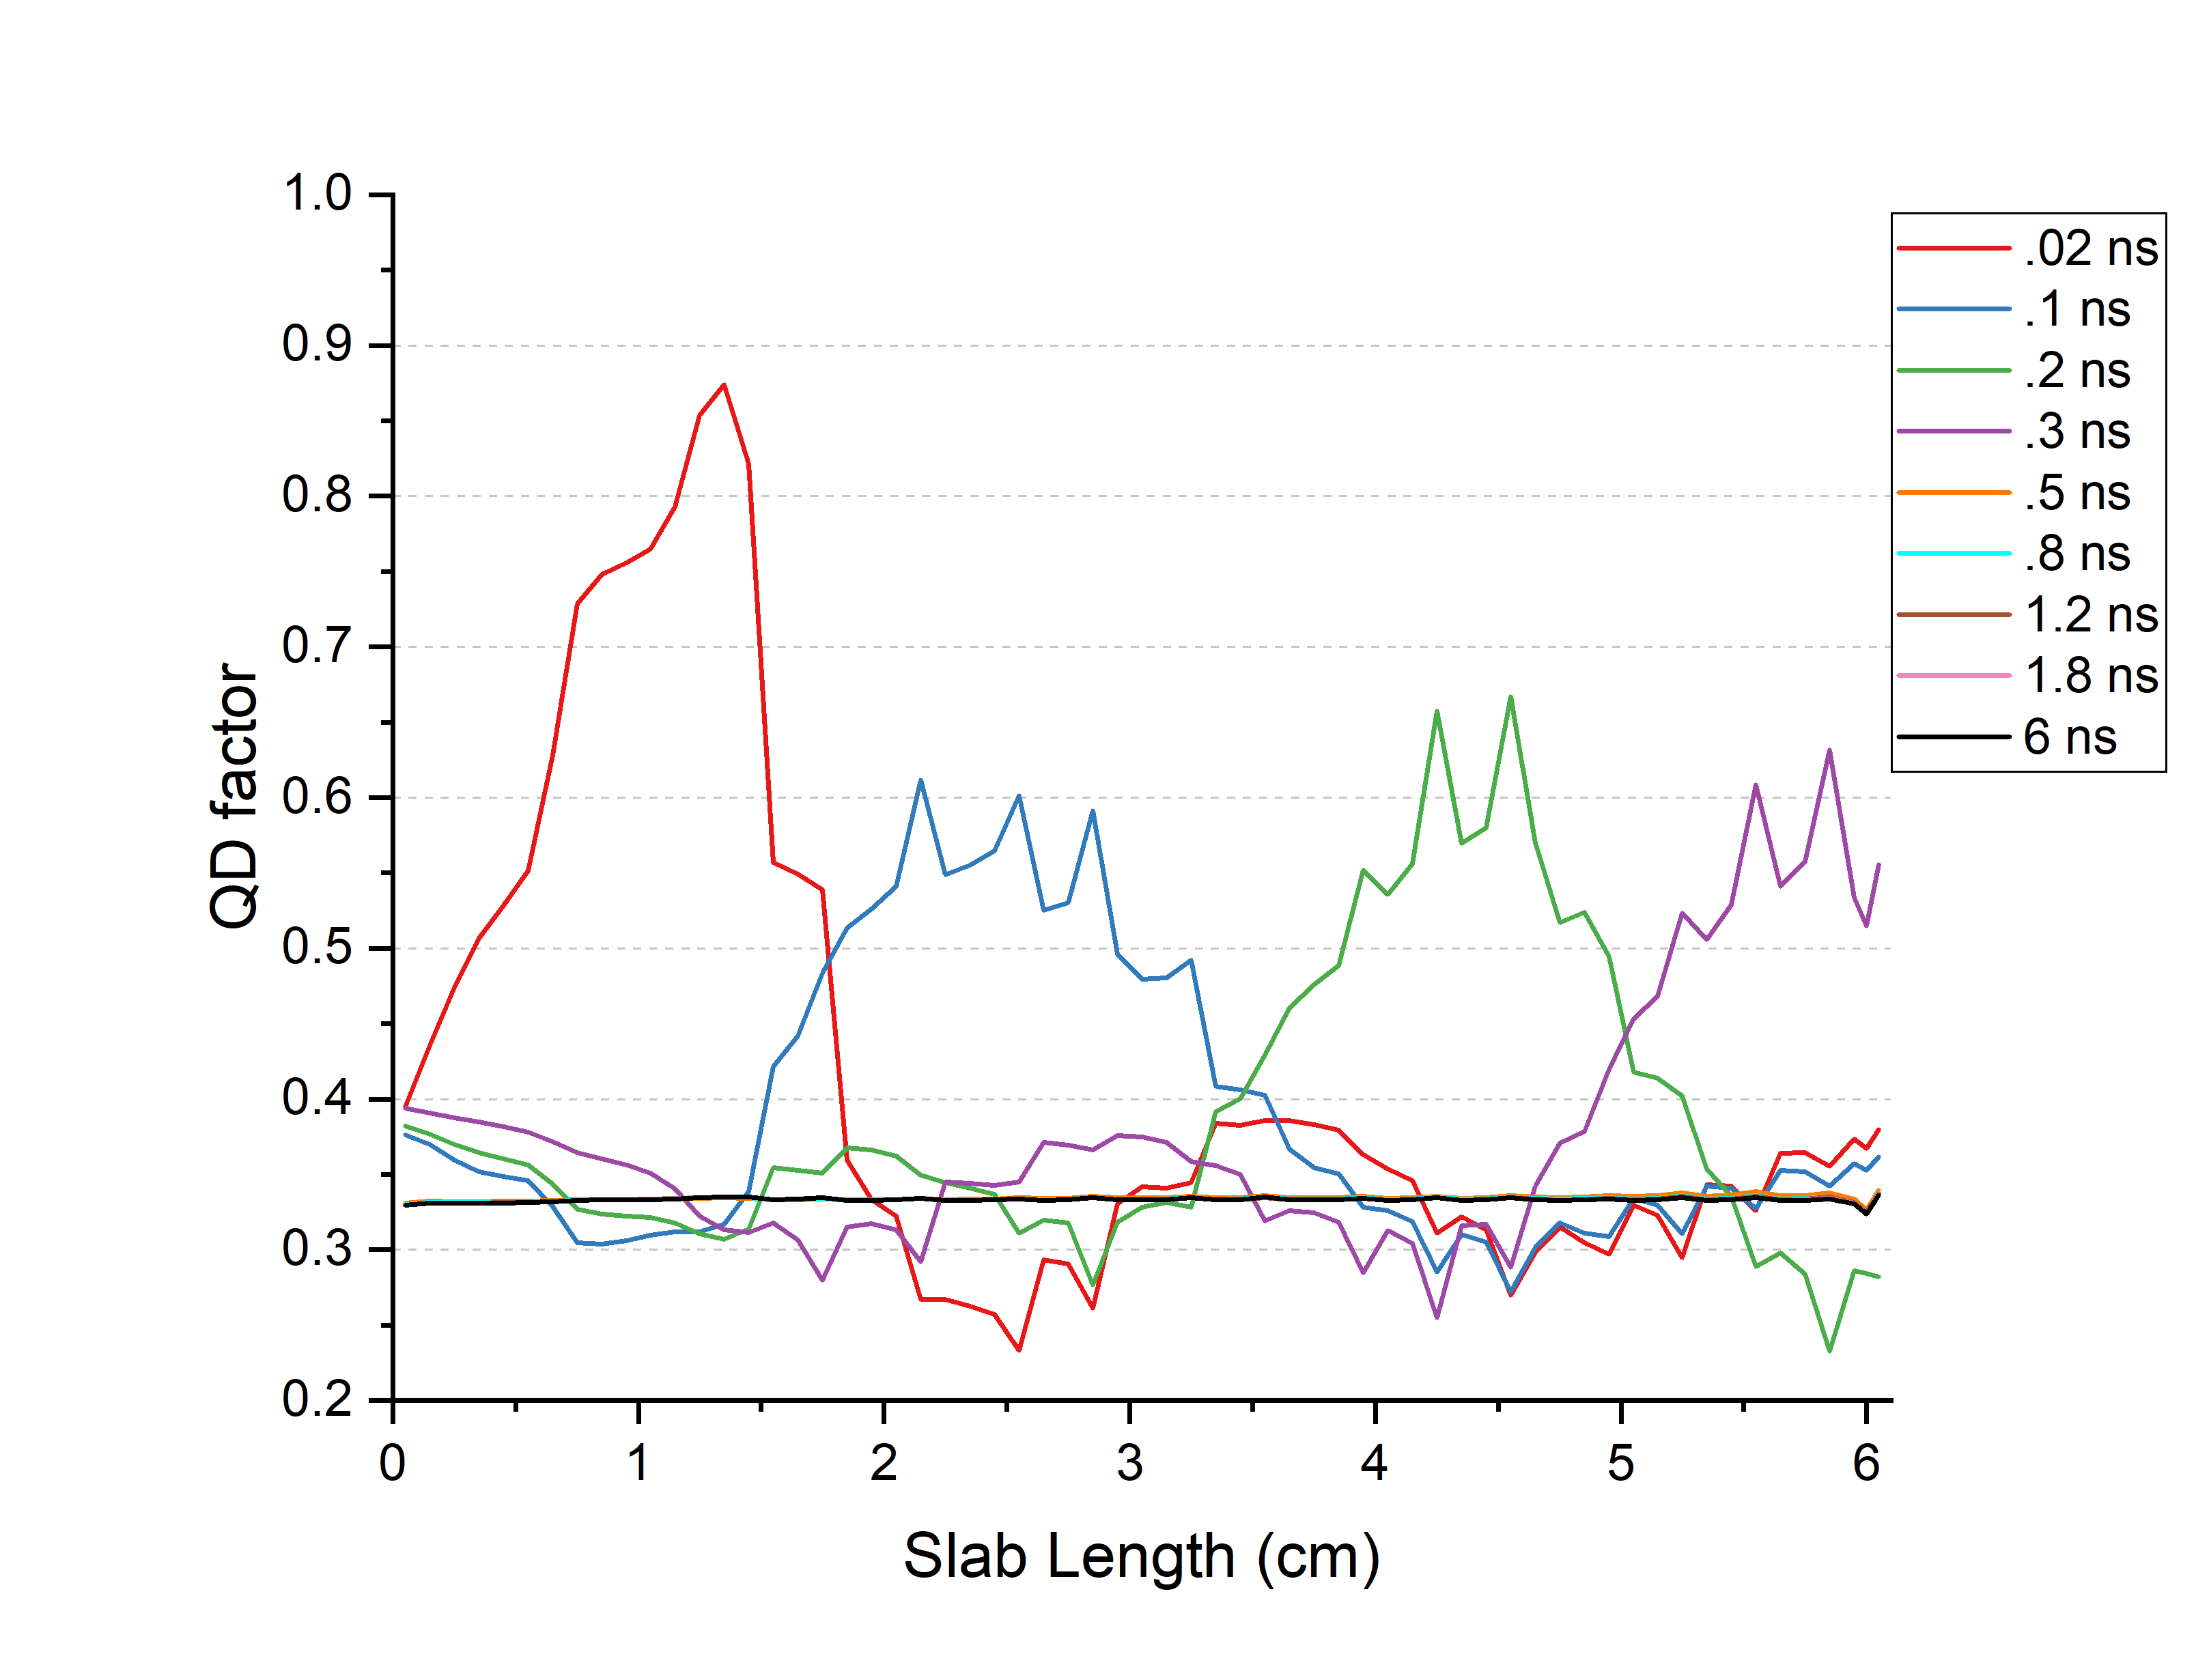
\includegraphics[width=0.5\textwidth]{qdf_g2_cut5.png}}
		\subfloat[r = 10 \label{subfig:qdf_g2_cut10}]{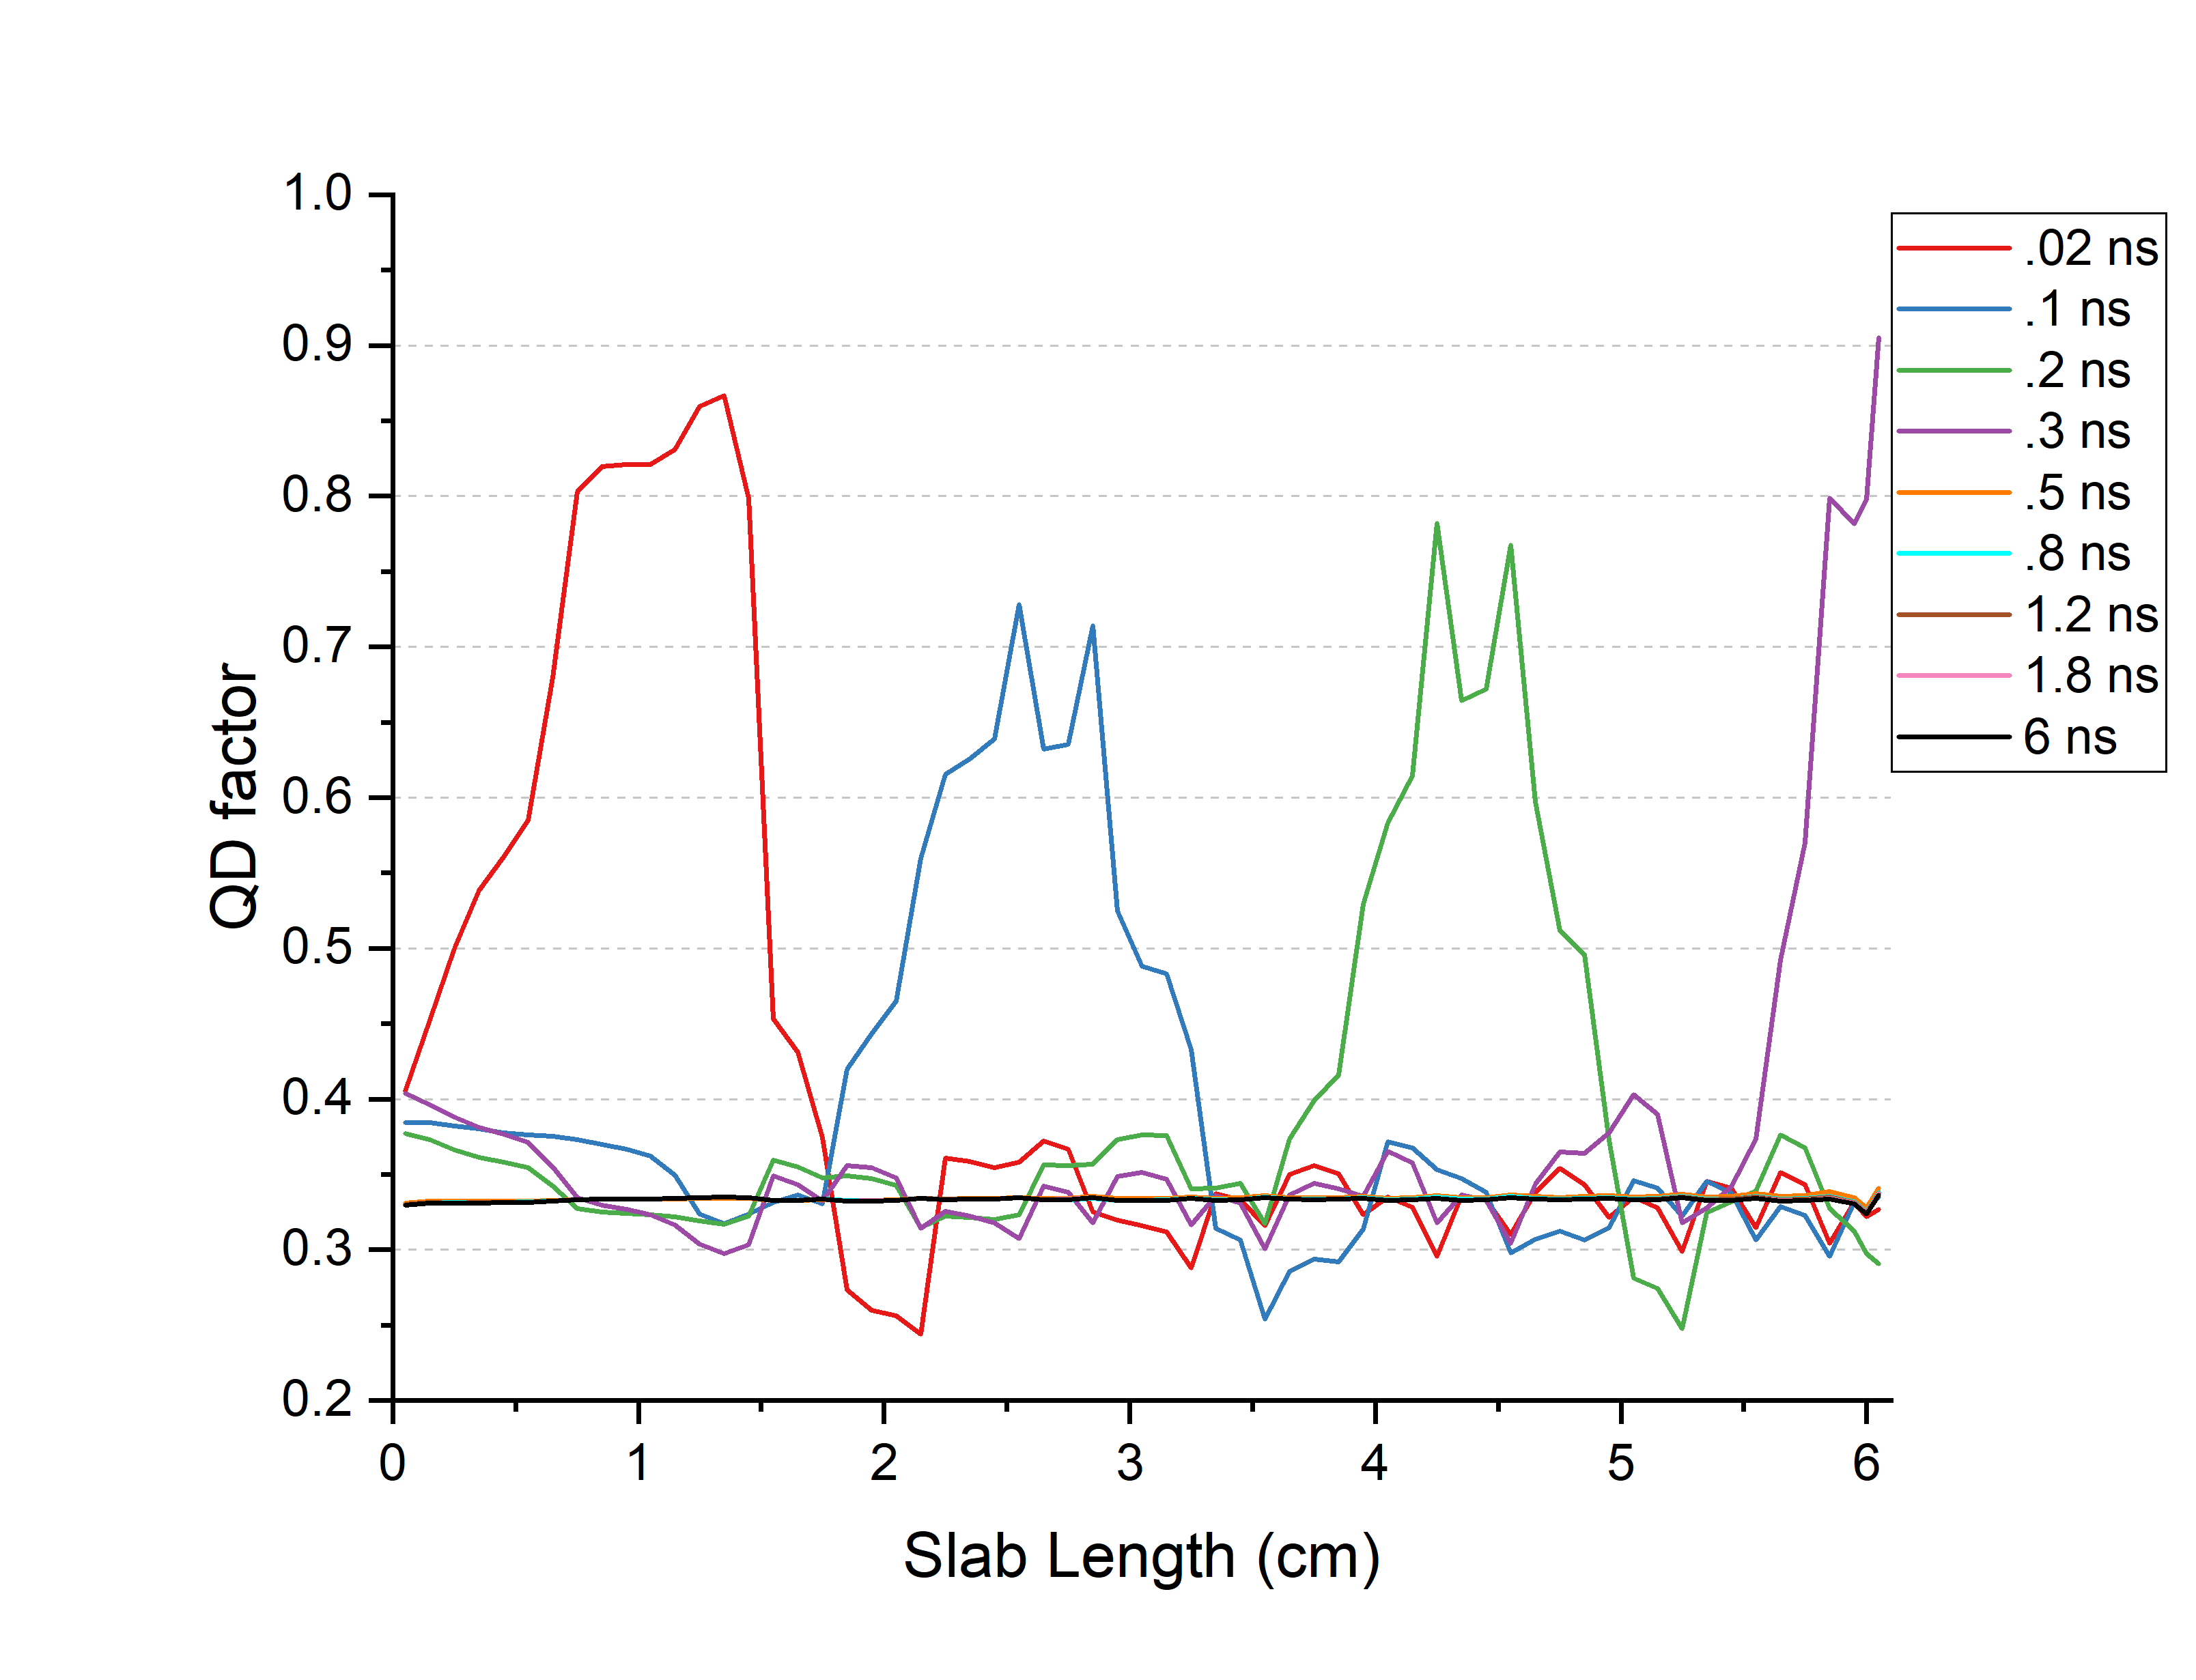
\includegraphics[width=0.5\textwidth]{qdf_g2_cut10.png}}\\
		\subfloat[r = 15 \label{subfig:qdf_g2_cut15}]{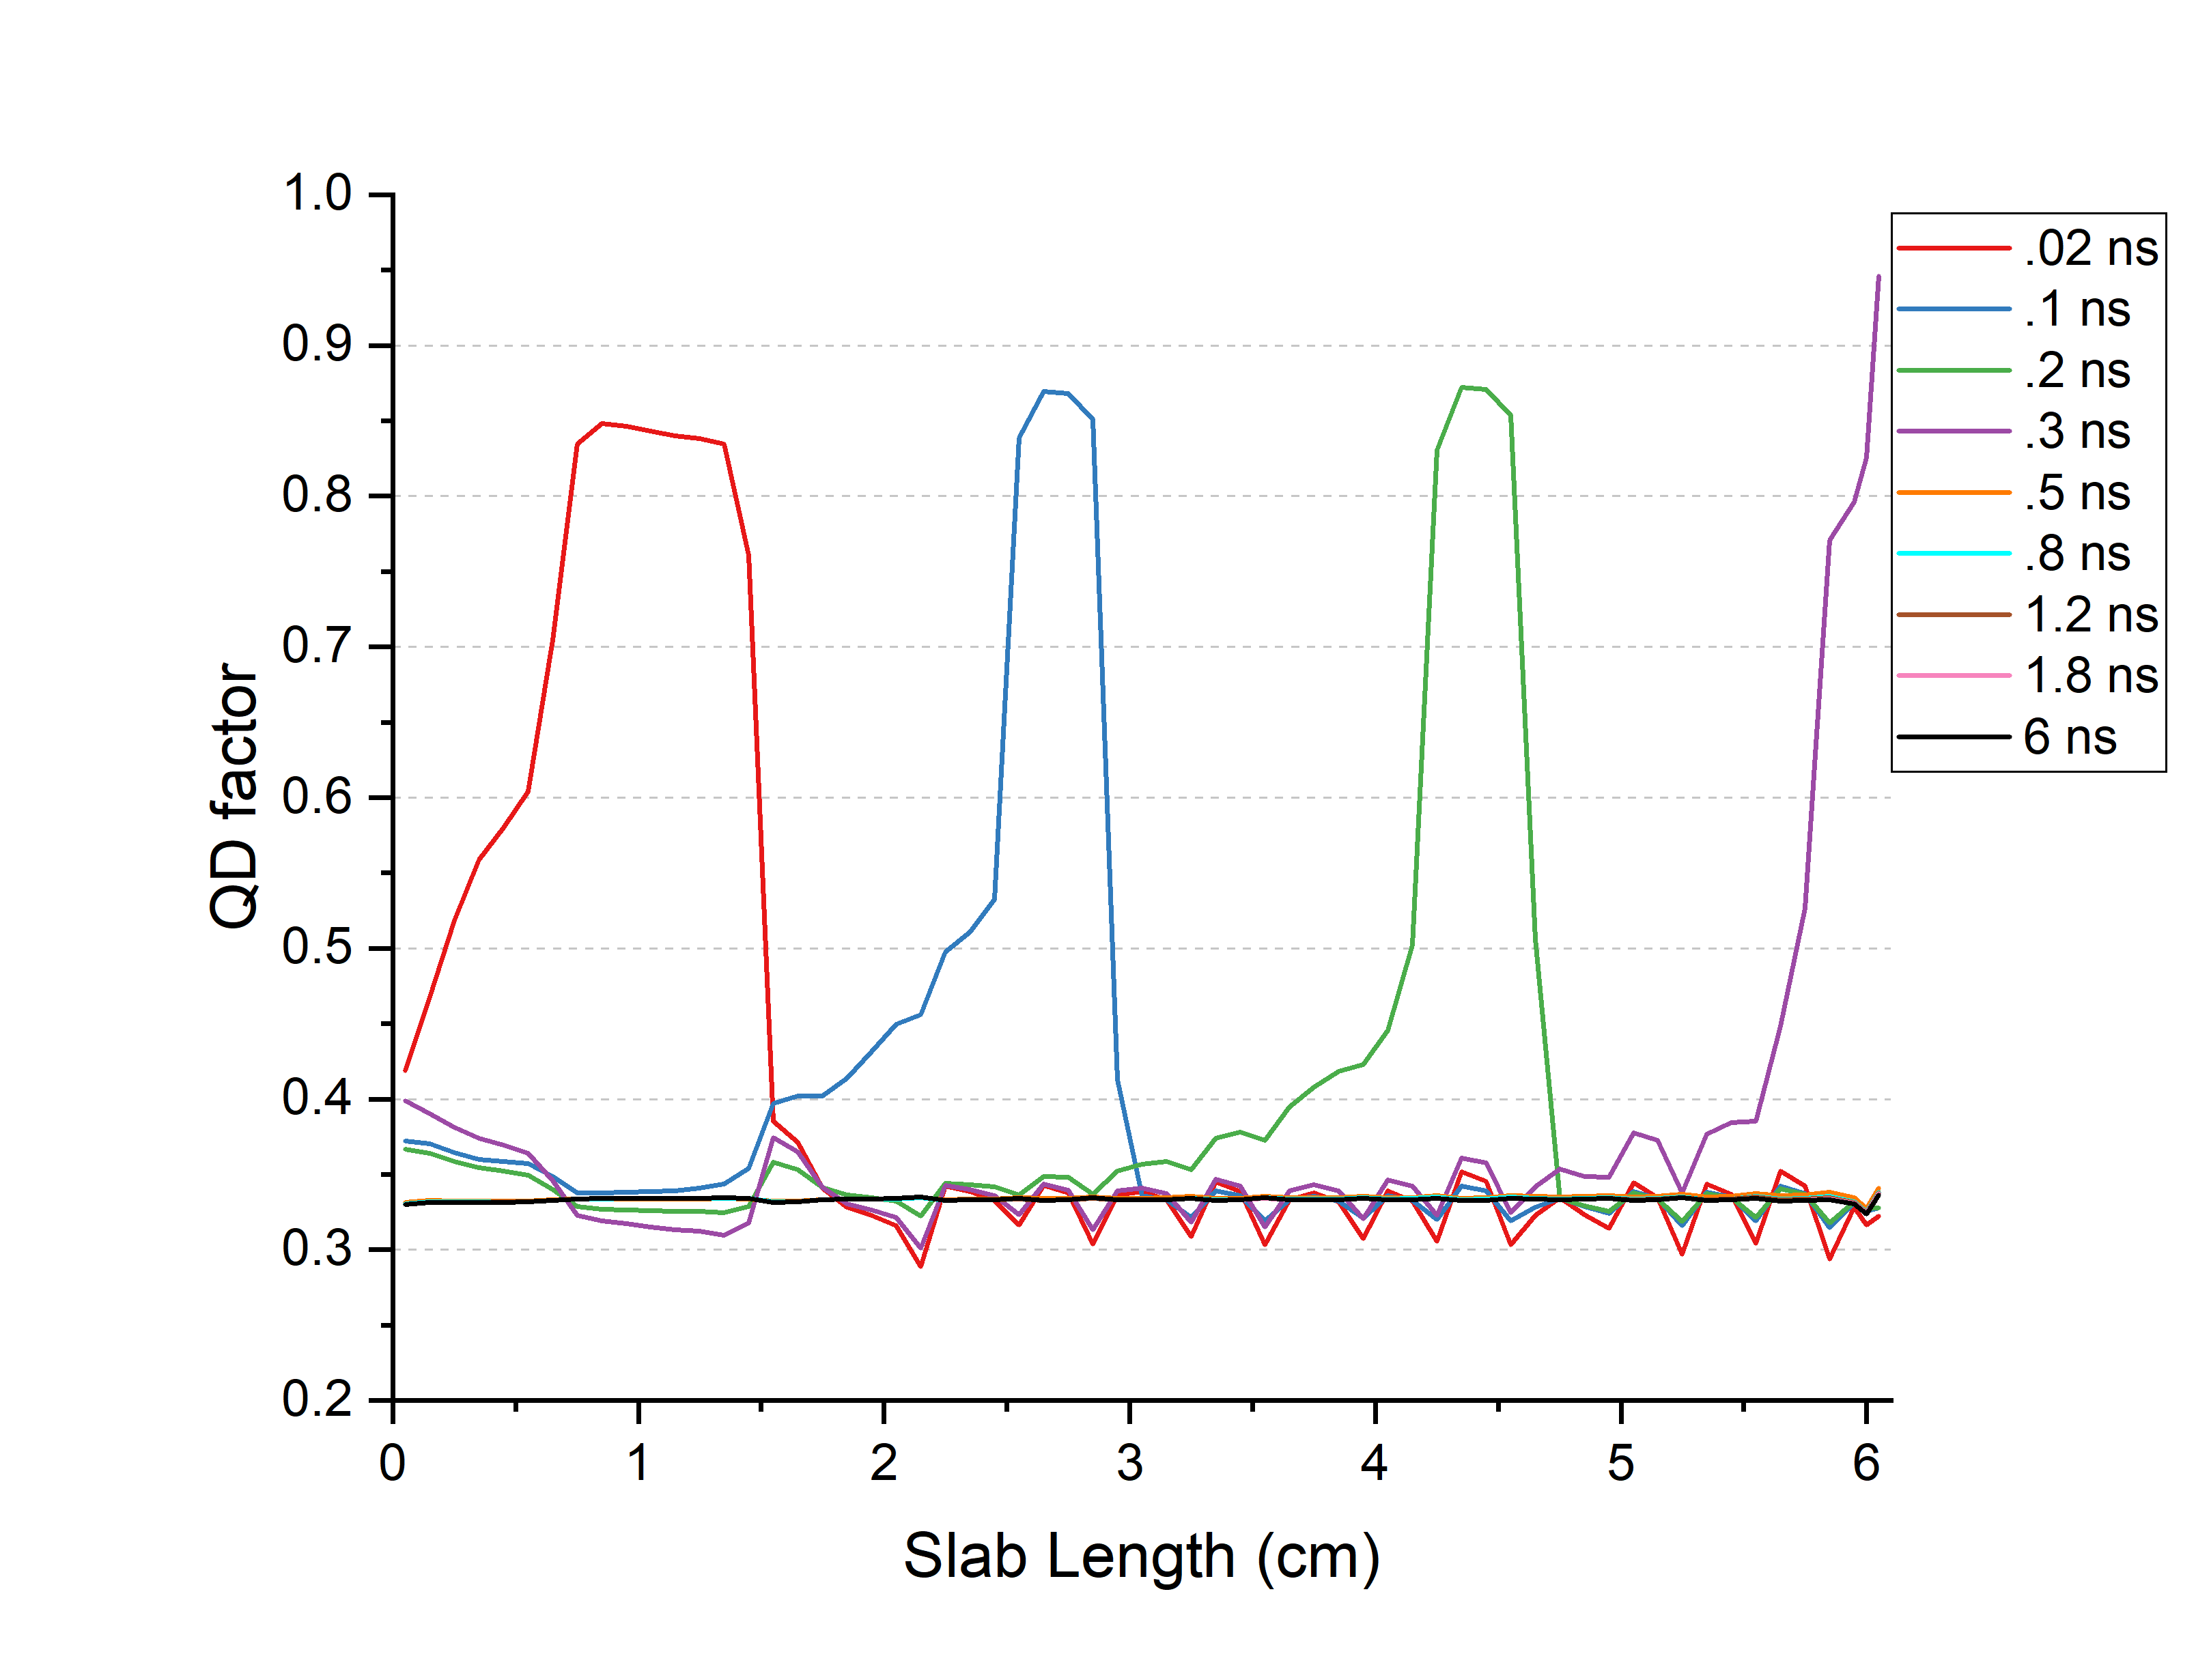
\includegraphics[width=0.5\textwidth]{qdf_g2_cut15.png}}
		\subfloat[r = 20 \label{subfig:qdf_g2_cut20}]{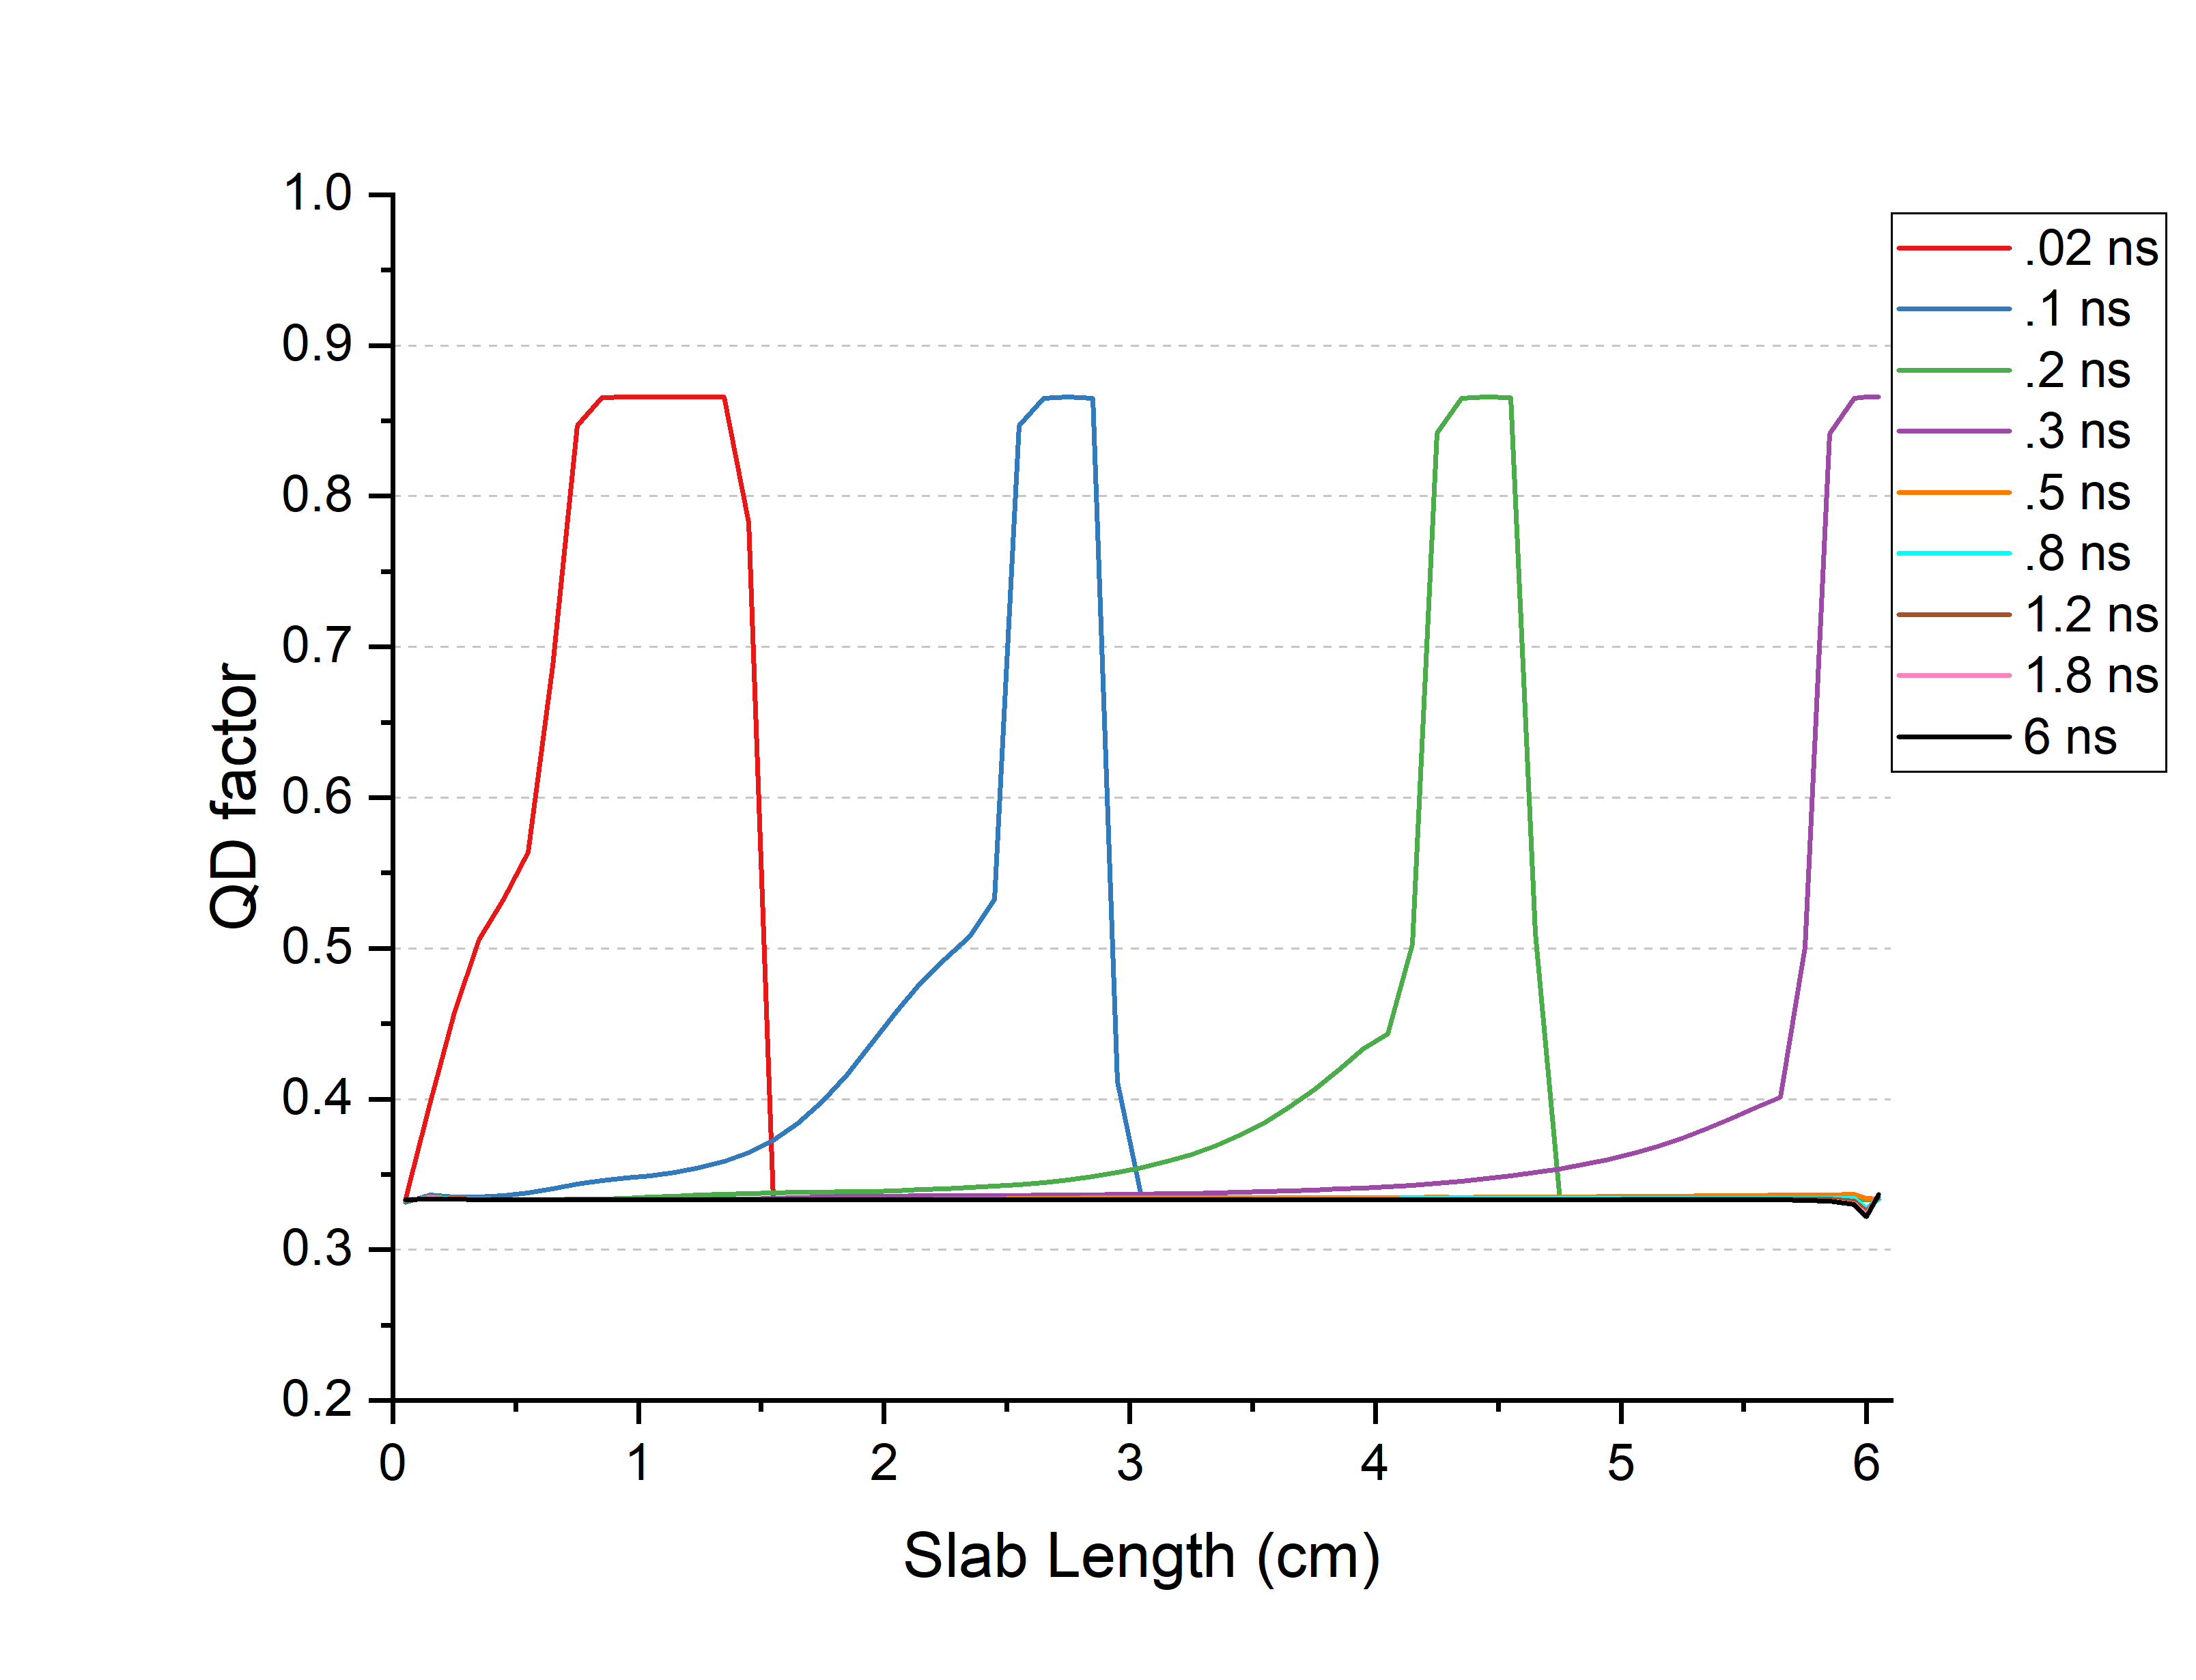
\includegraphics[width=0.5\textwidth]{qdf_g2_cut20.png}}
		\caption{\label{fig:qdf_g2_recomps}
			Low-rank approximation of the group QD factors for $g=2$ for select time steps}
	\end{figure}

	%=================================================================================
	% QDF G3 RECOMP
	\begin{figure}[ht!]
		\centering
		\subfloat[r = 1 \label{subfig:qdf_g3_cut1}]{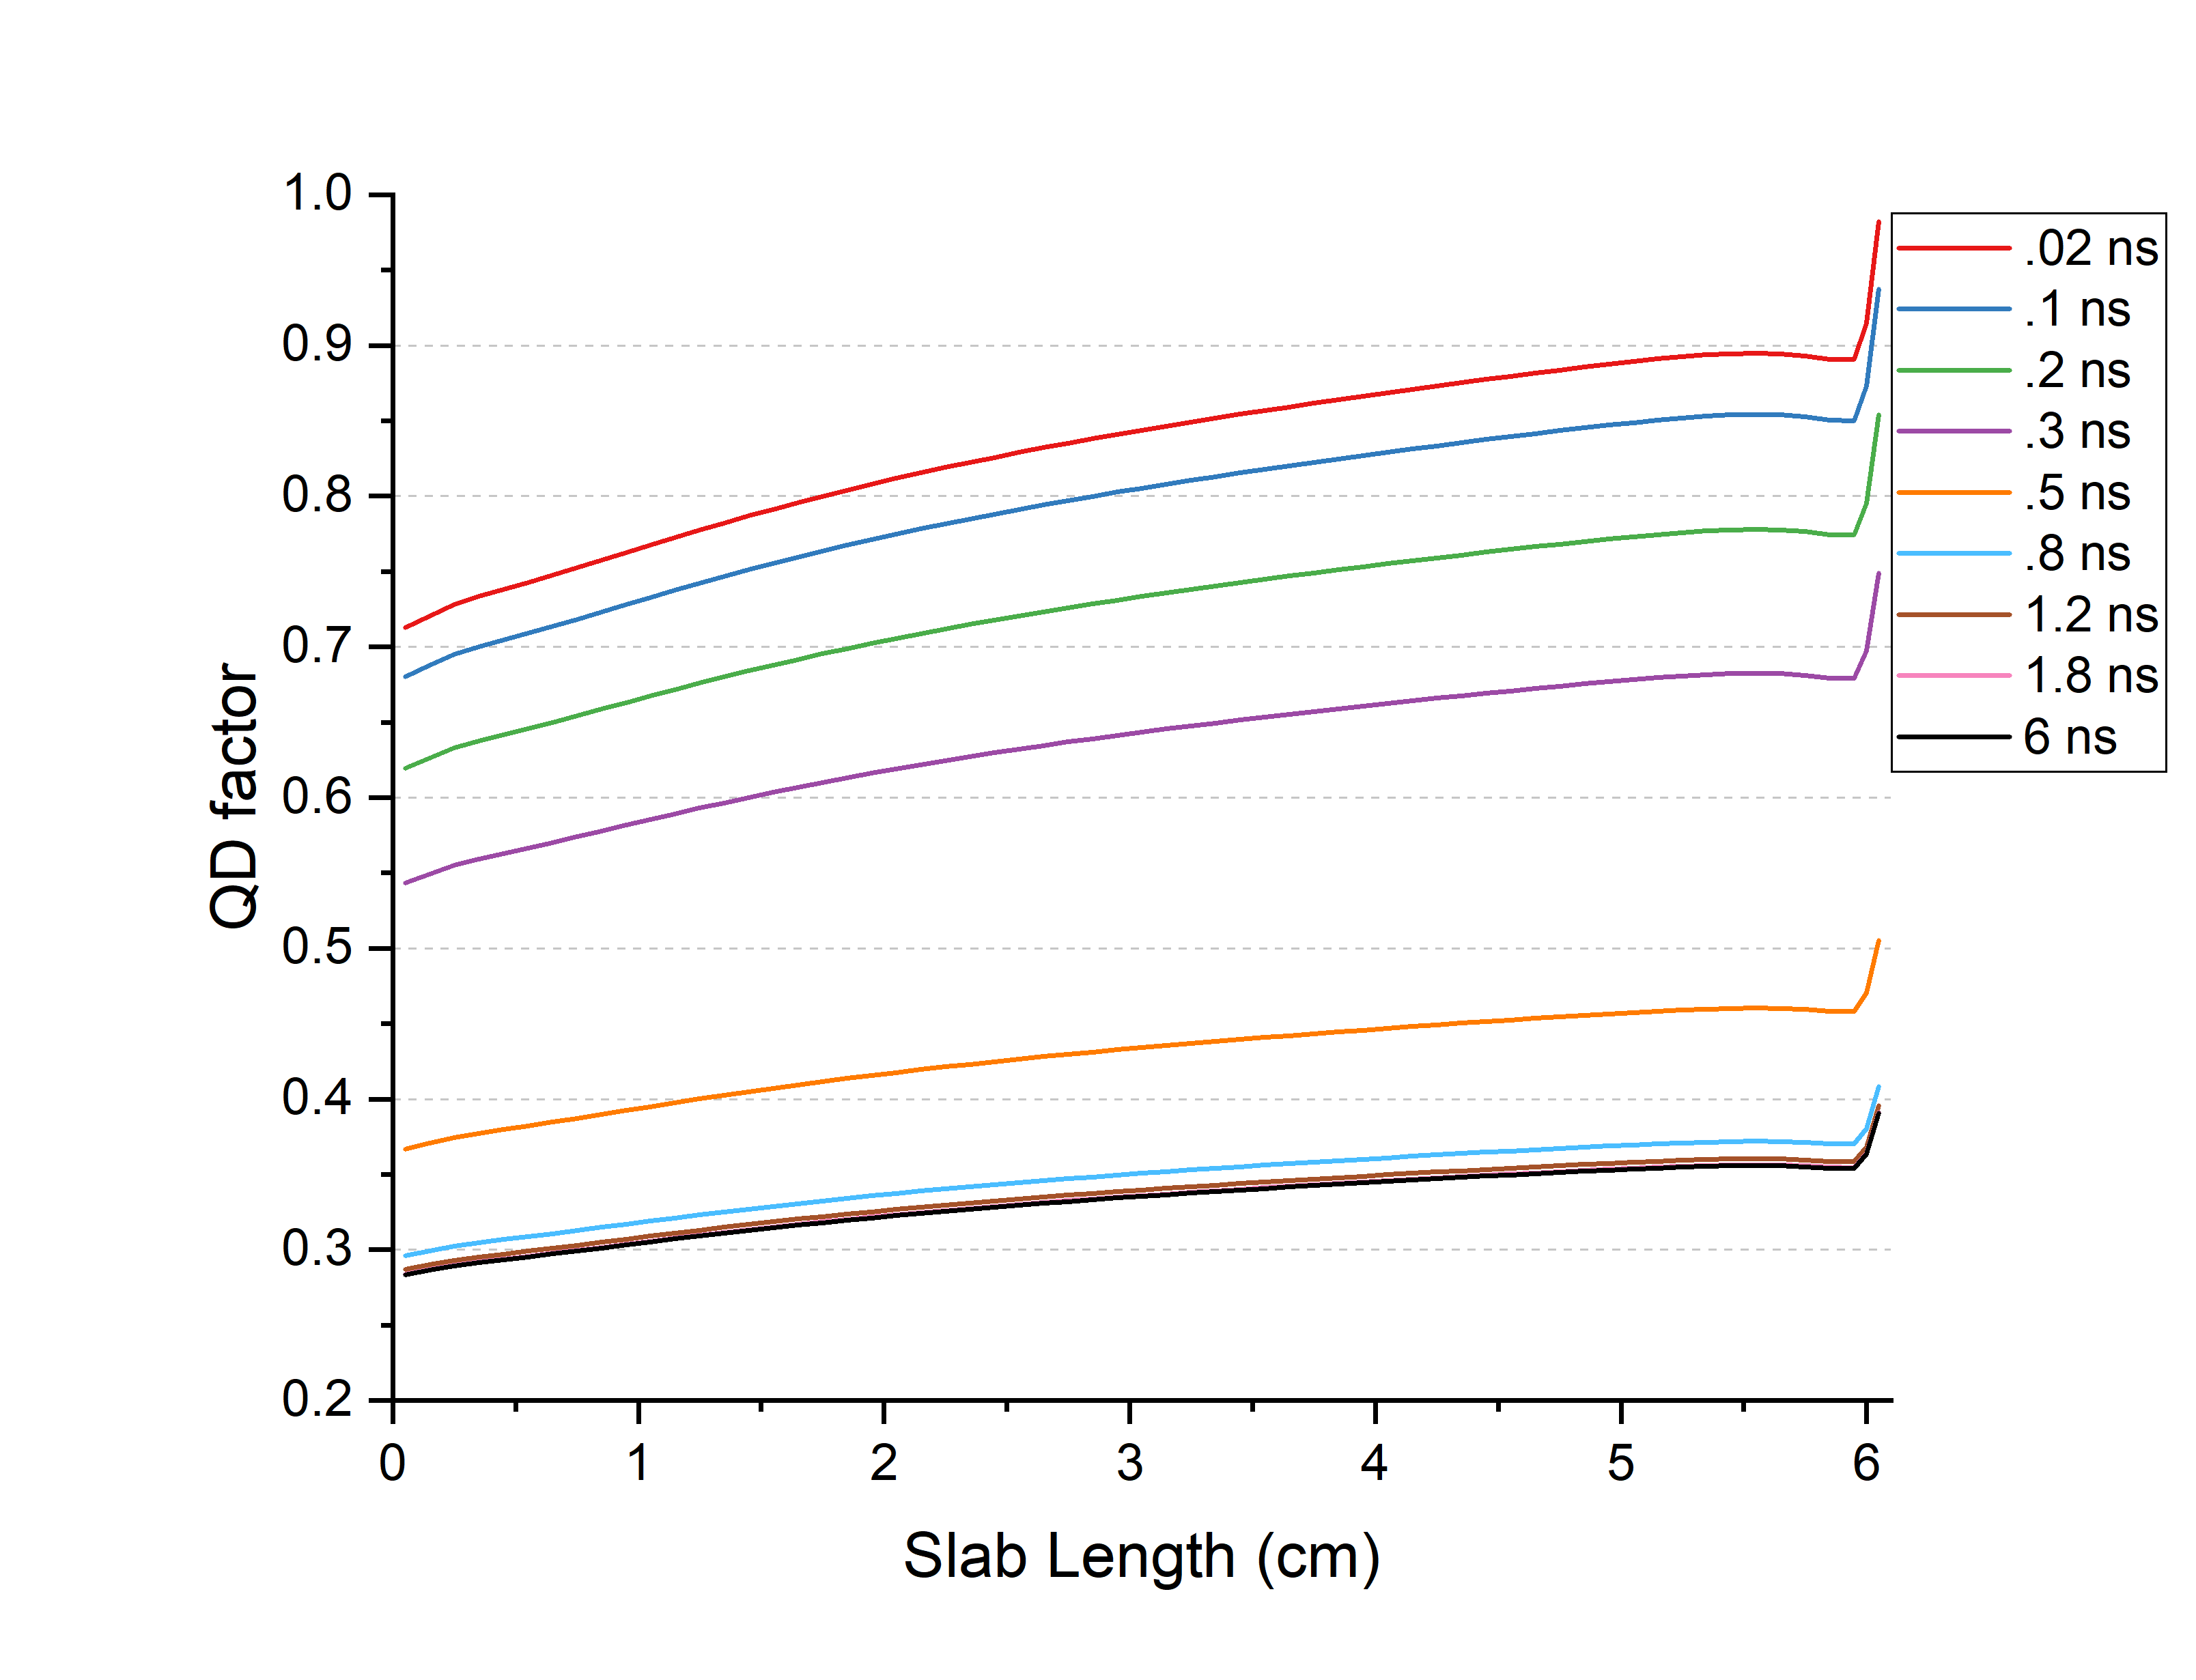
\includegraphics[width=0.5\textwidth]{qdf_g3_cut1.png}}
		\subfloat[r = 2 \label{subfig:qdf_g3_cut2}]{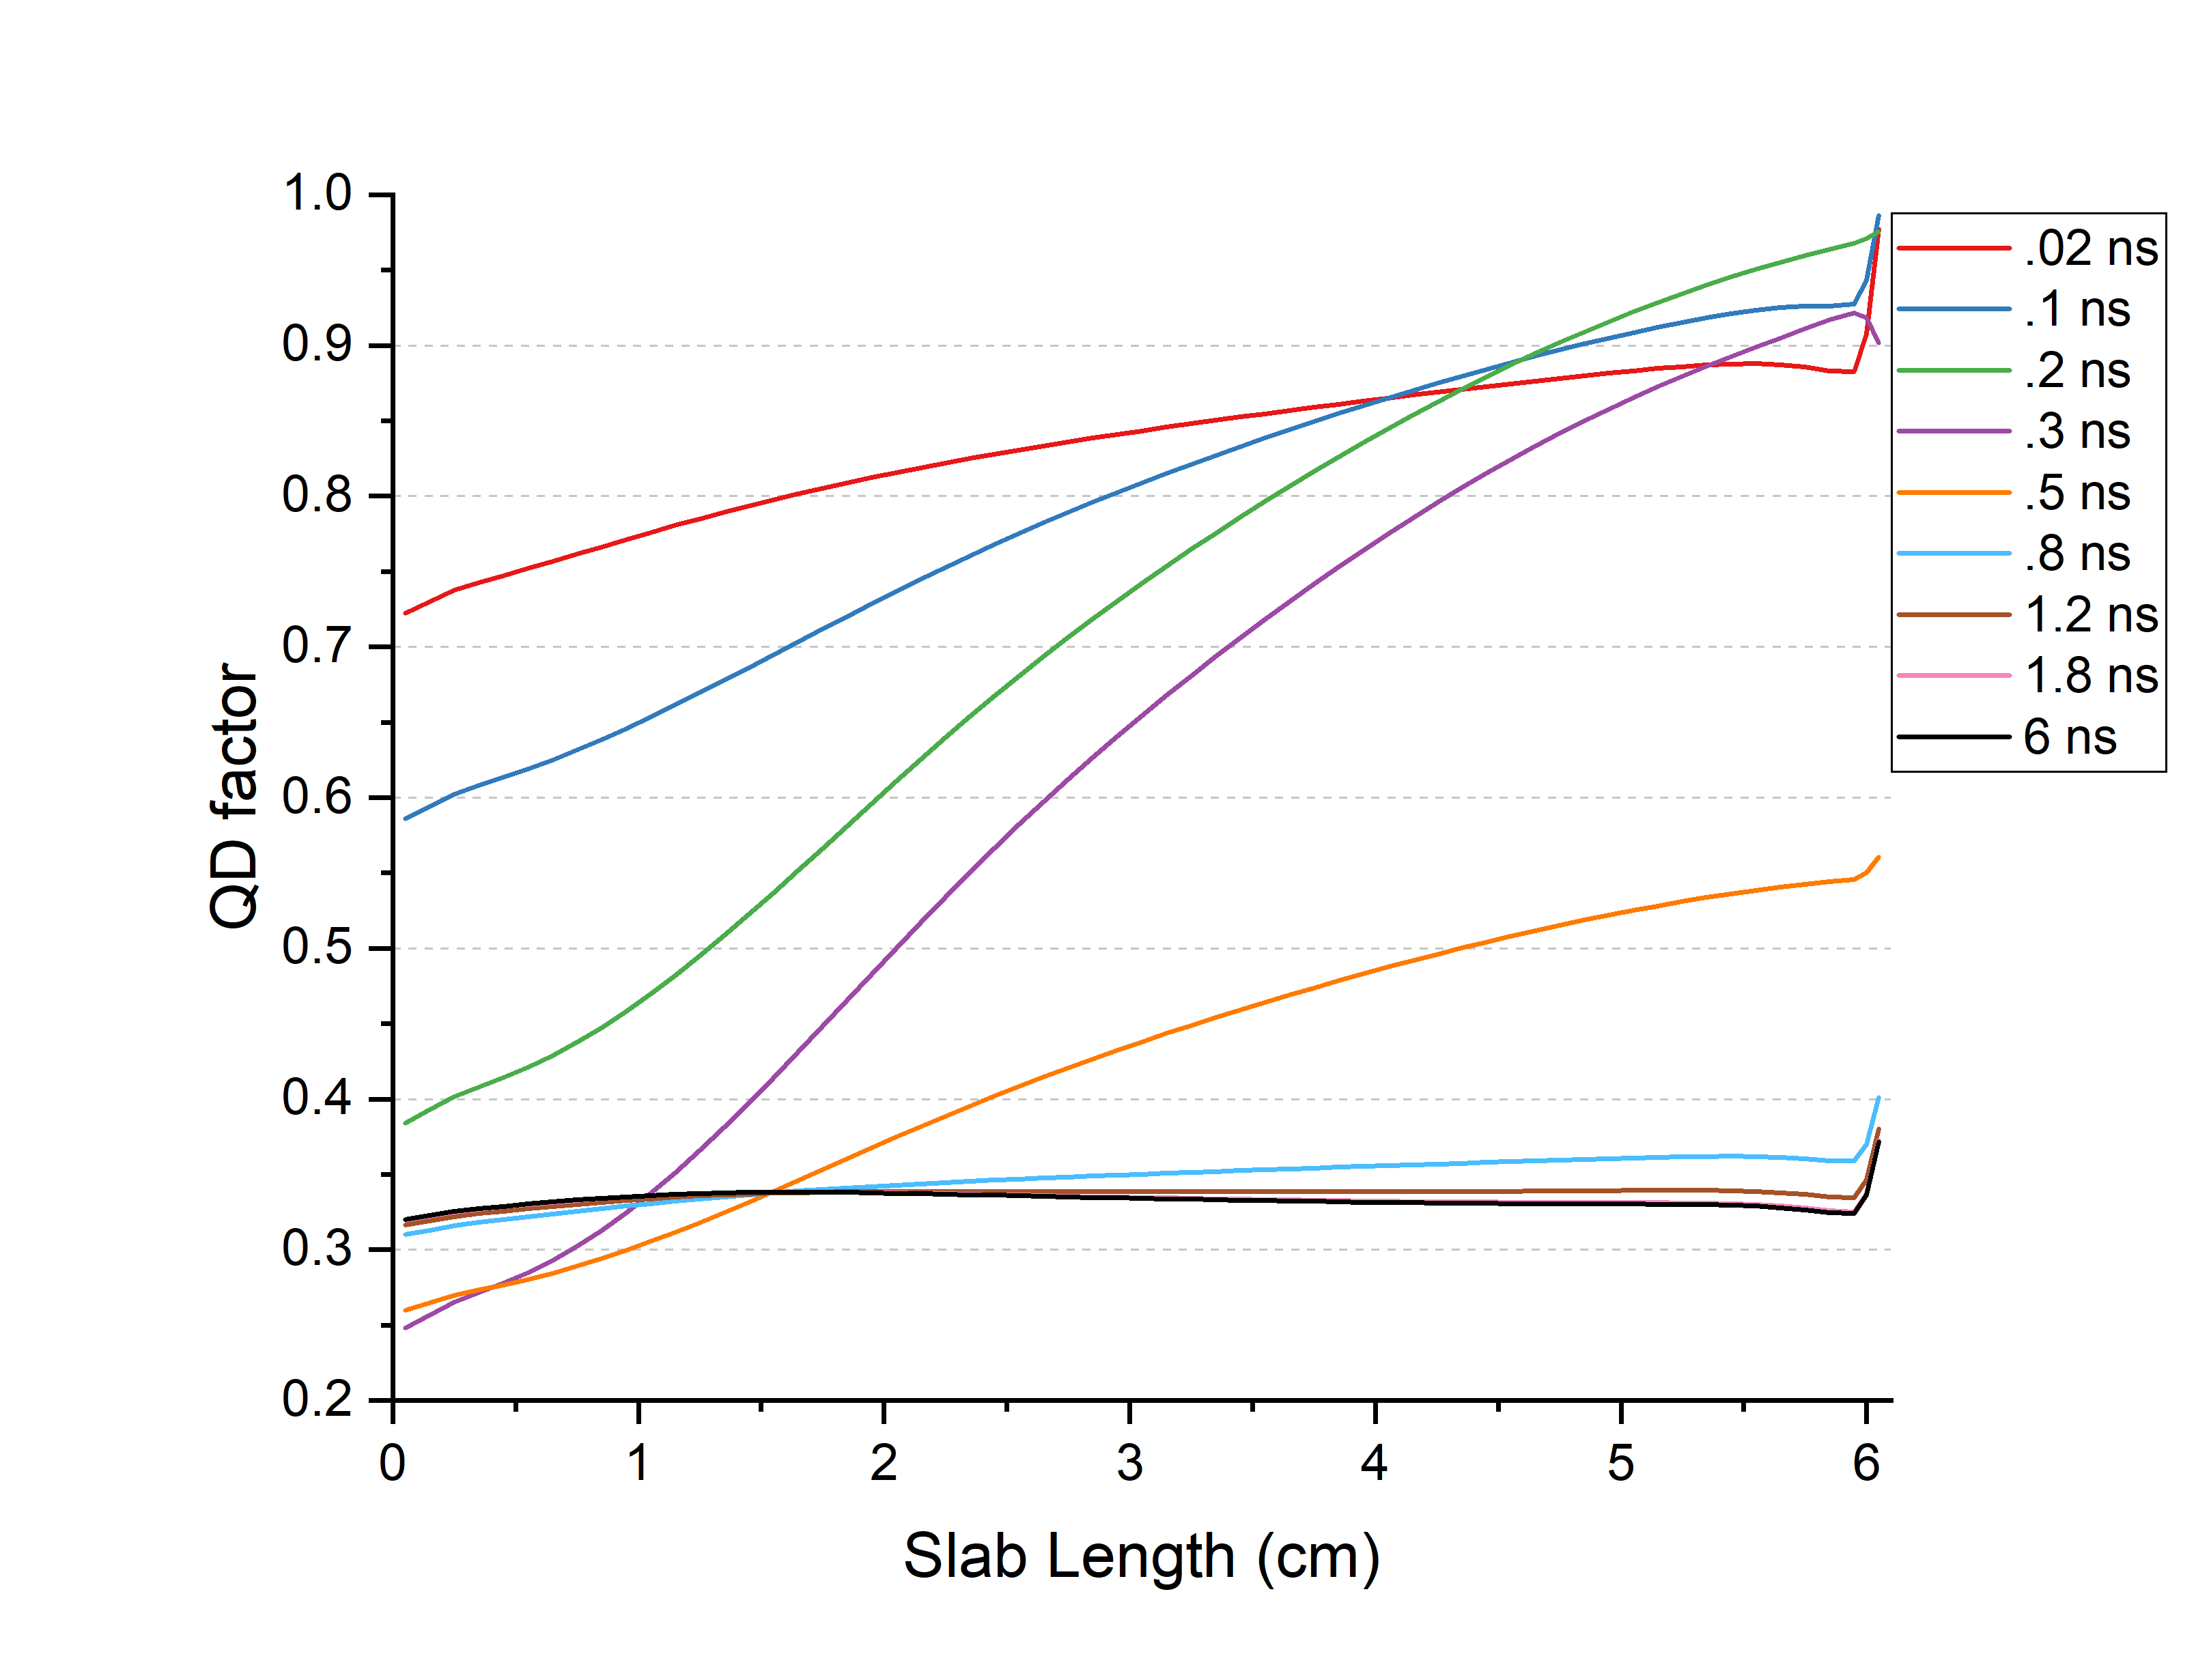
\includegraphics[width=0.5\textwidth]{qdf_g3_cut2.png}}\\
		\subfloat[r = 5 \label{subfig:qdf_g3_cut5}]{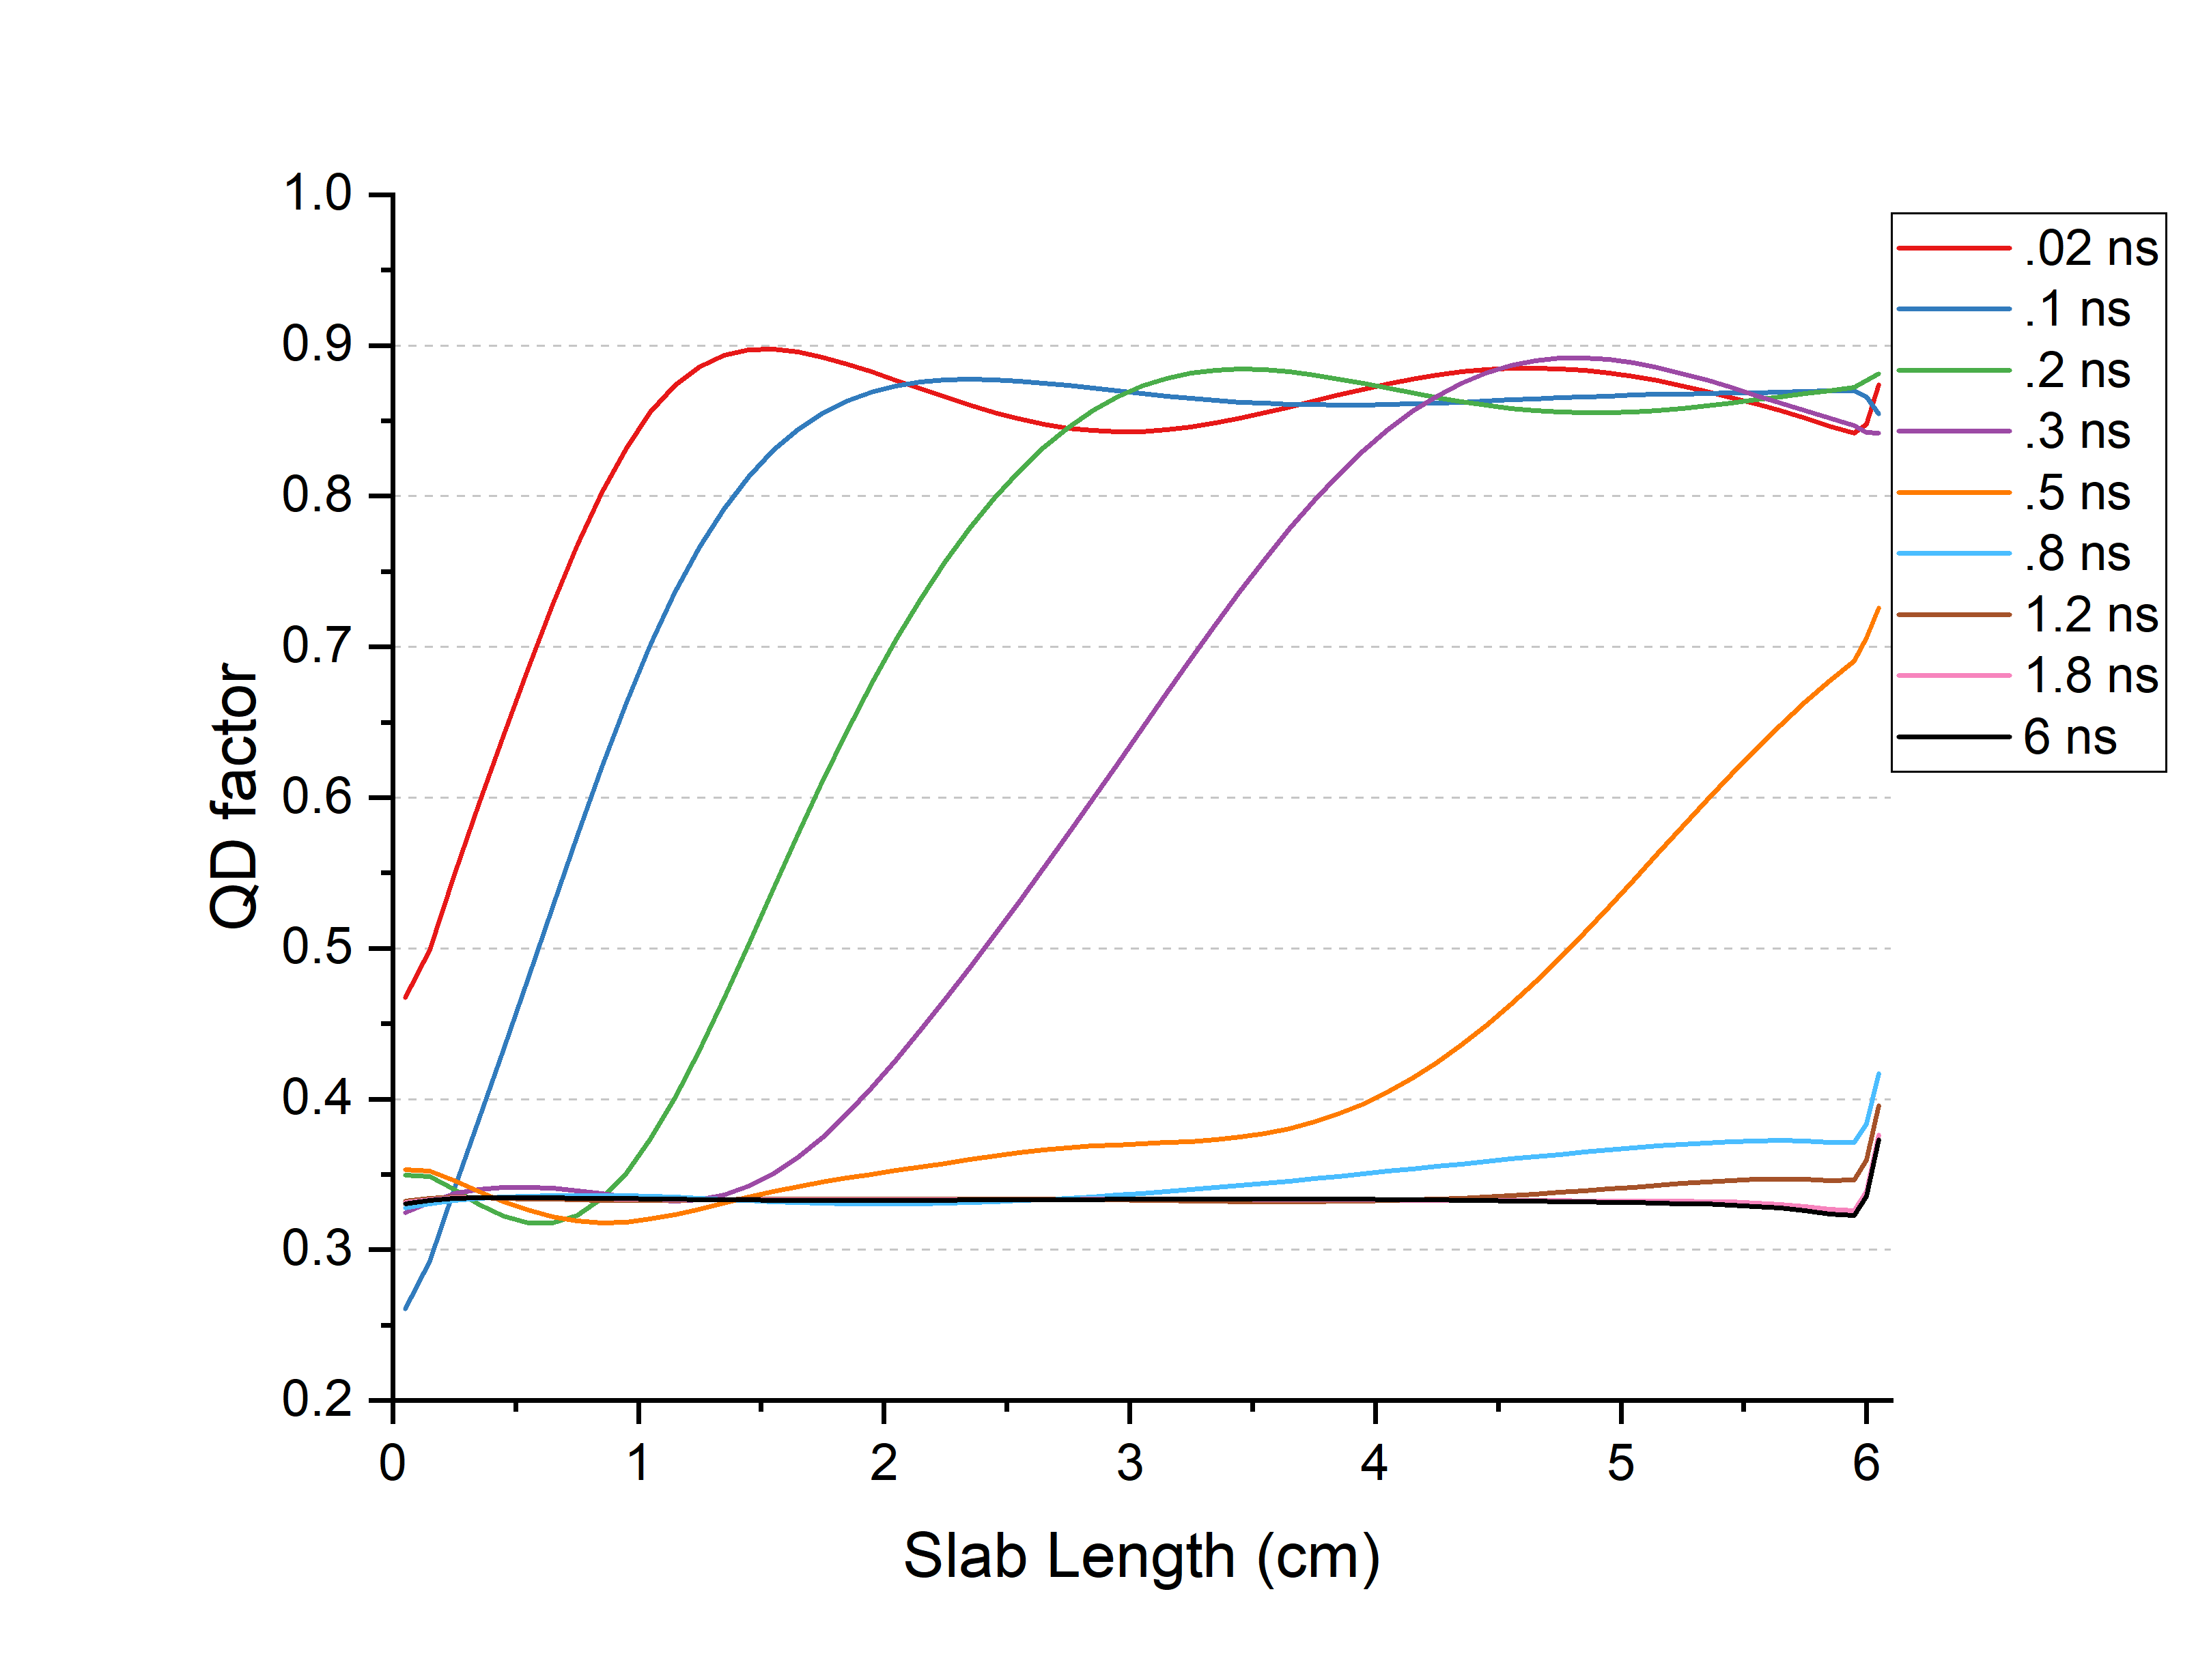
\includegraphics[width=0.5\textwidth]{qdf_g3_cut5.png}}
		\subfloat[r = 10 \label{subfig:qdf_g3_cut10}]{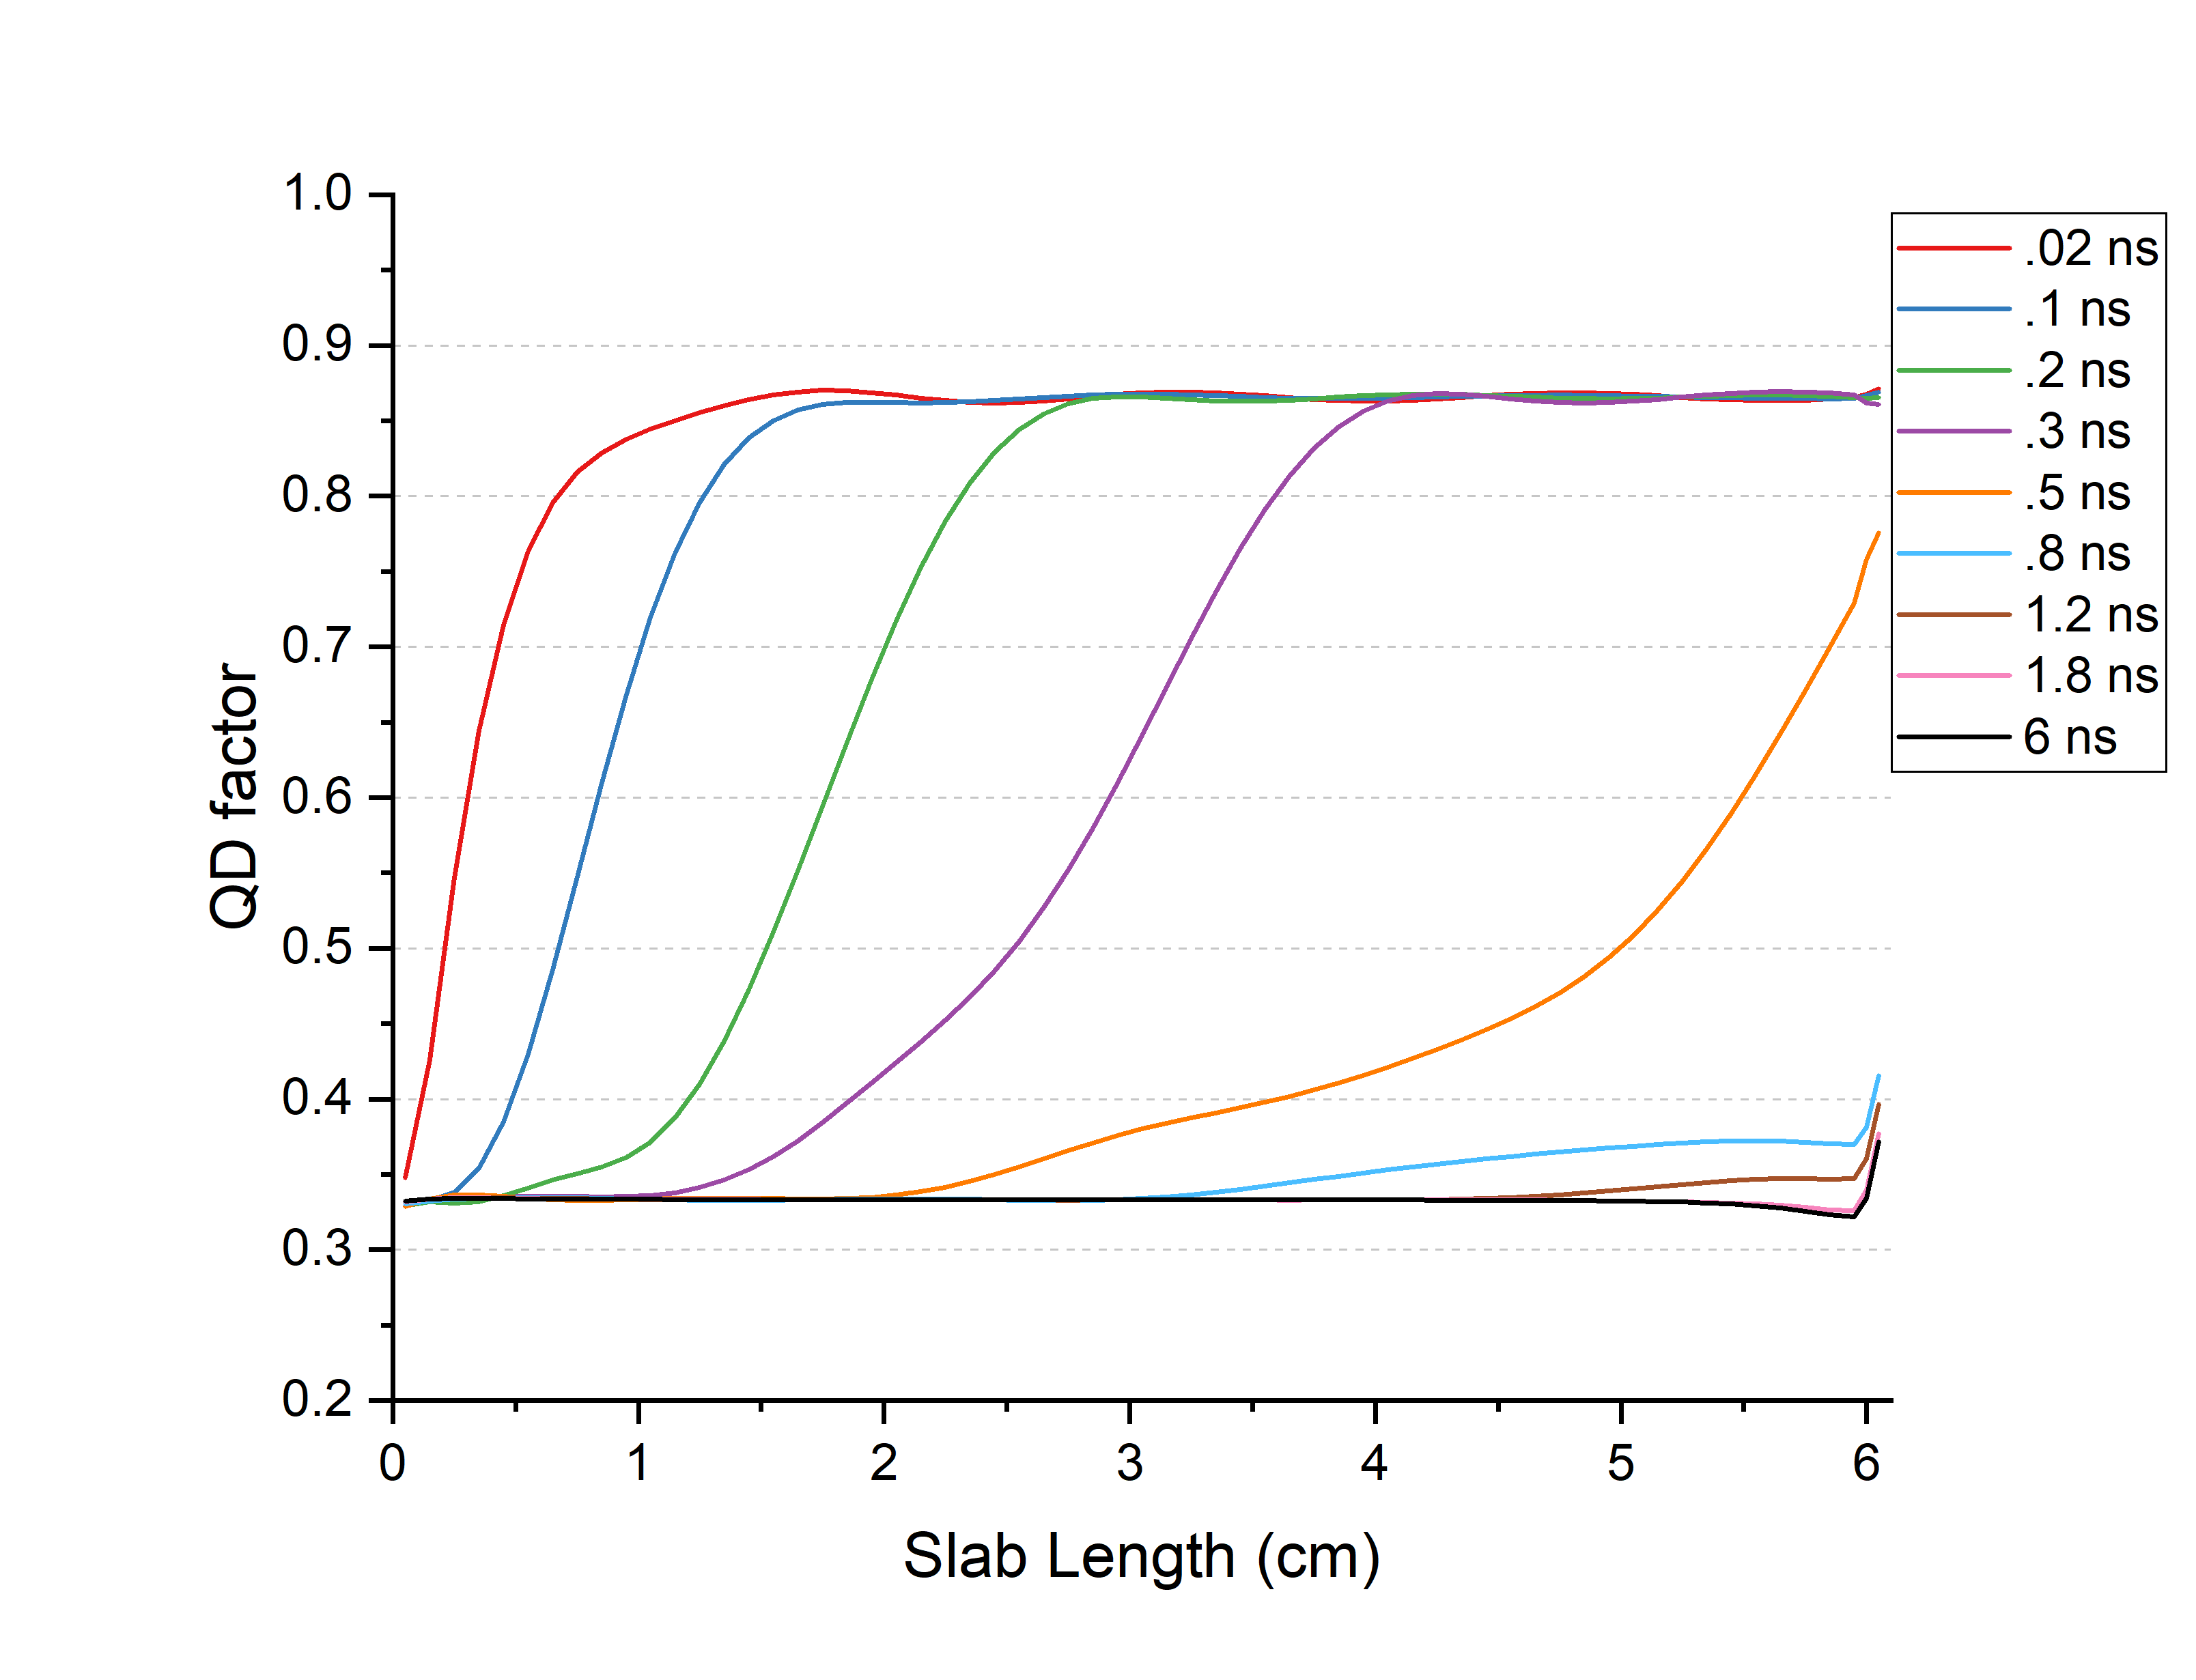
\includegraphics[width=0.5\textwidth]{qdf_g3_cut10.png}}\\
		\subfloat[r = 15 \label{subfig:qdf_g3_cut15}]{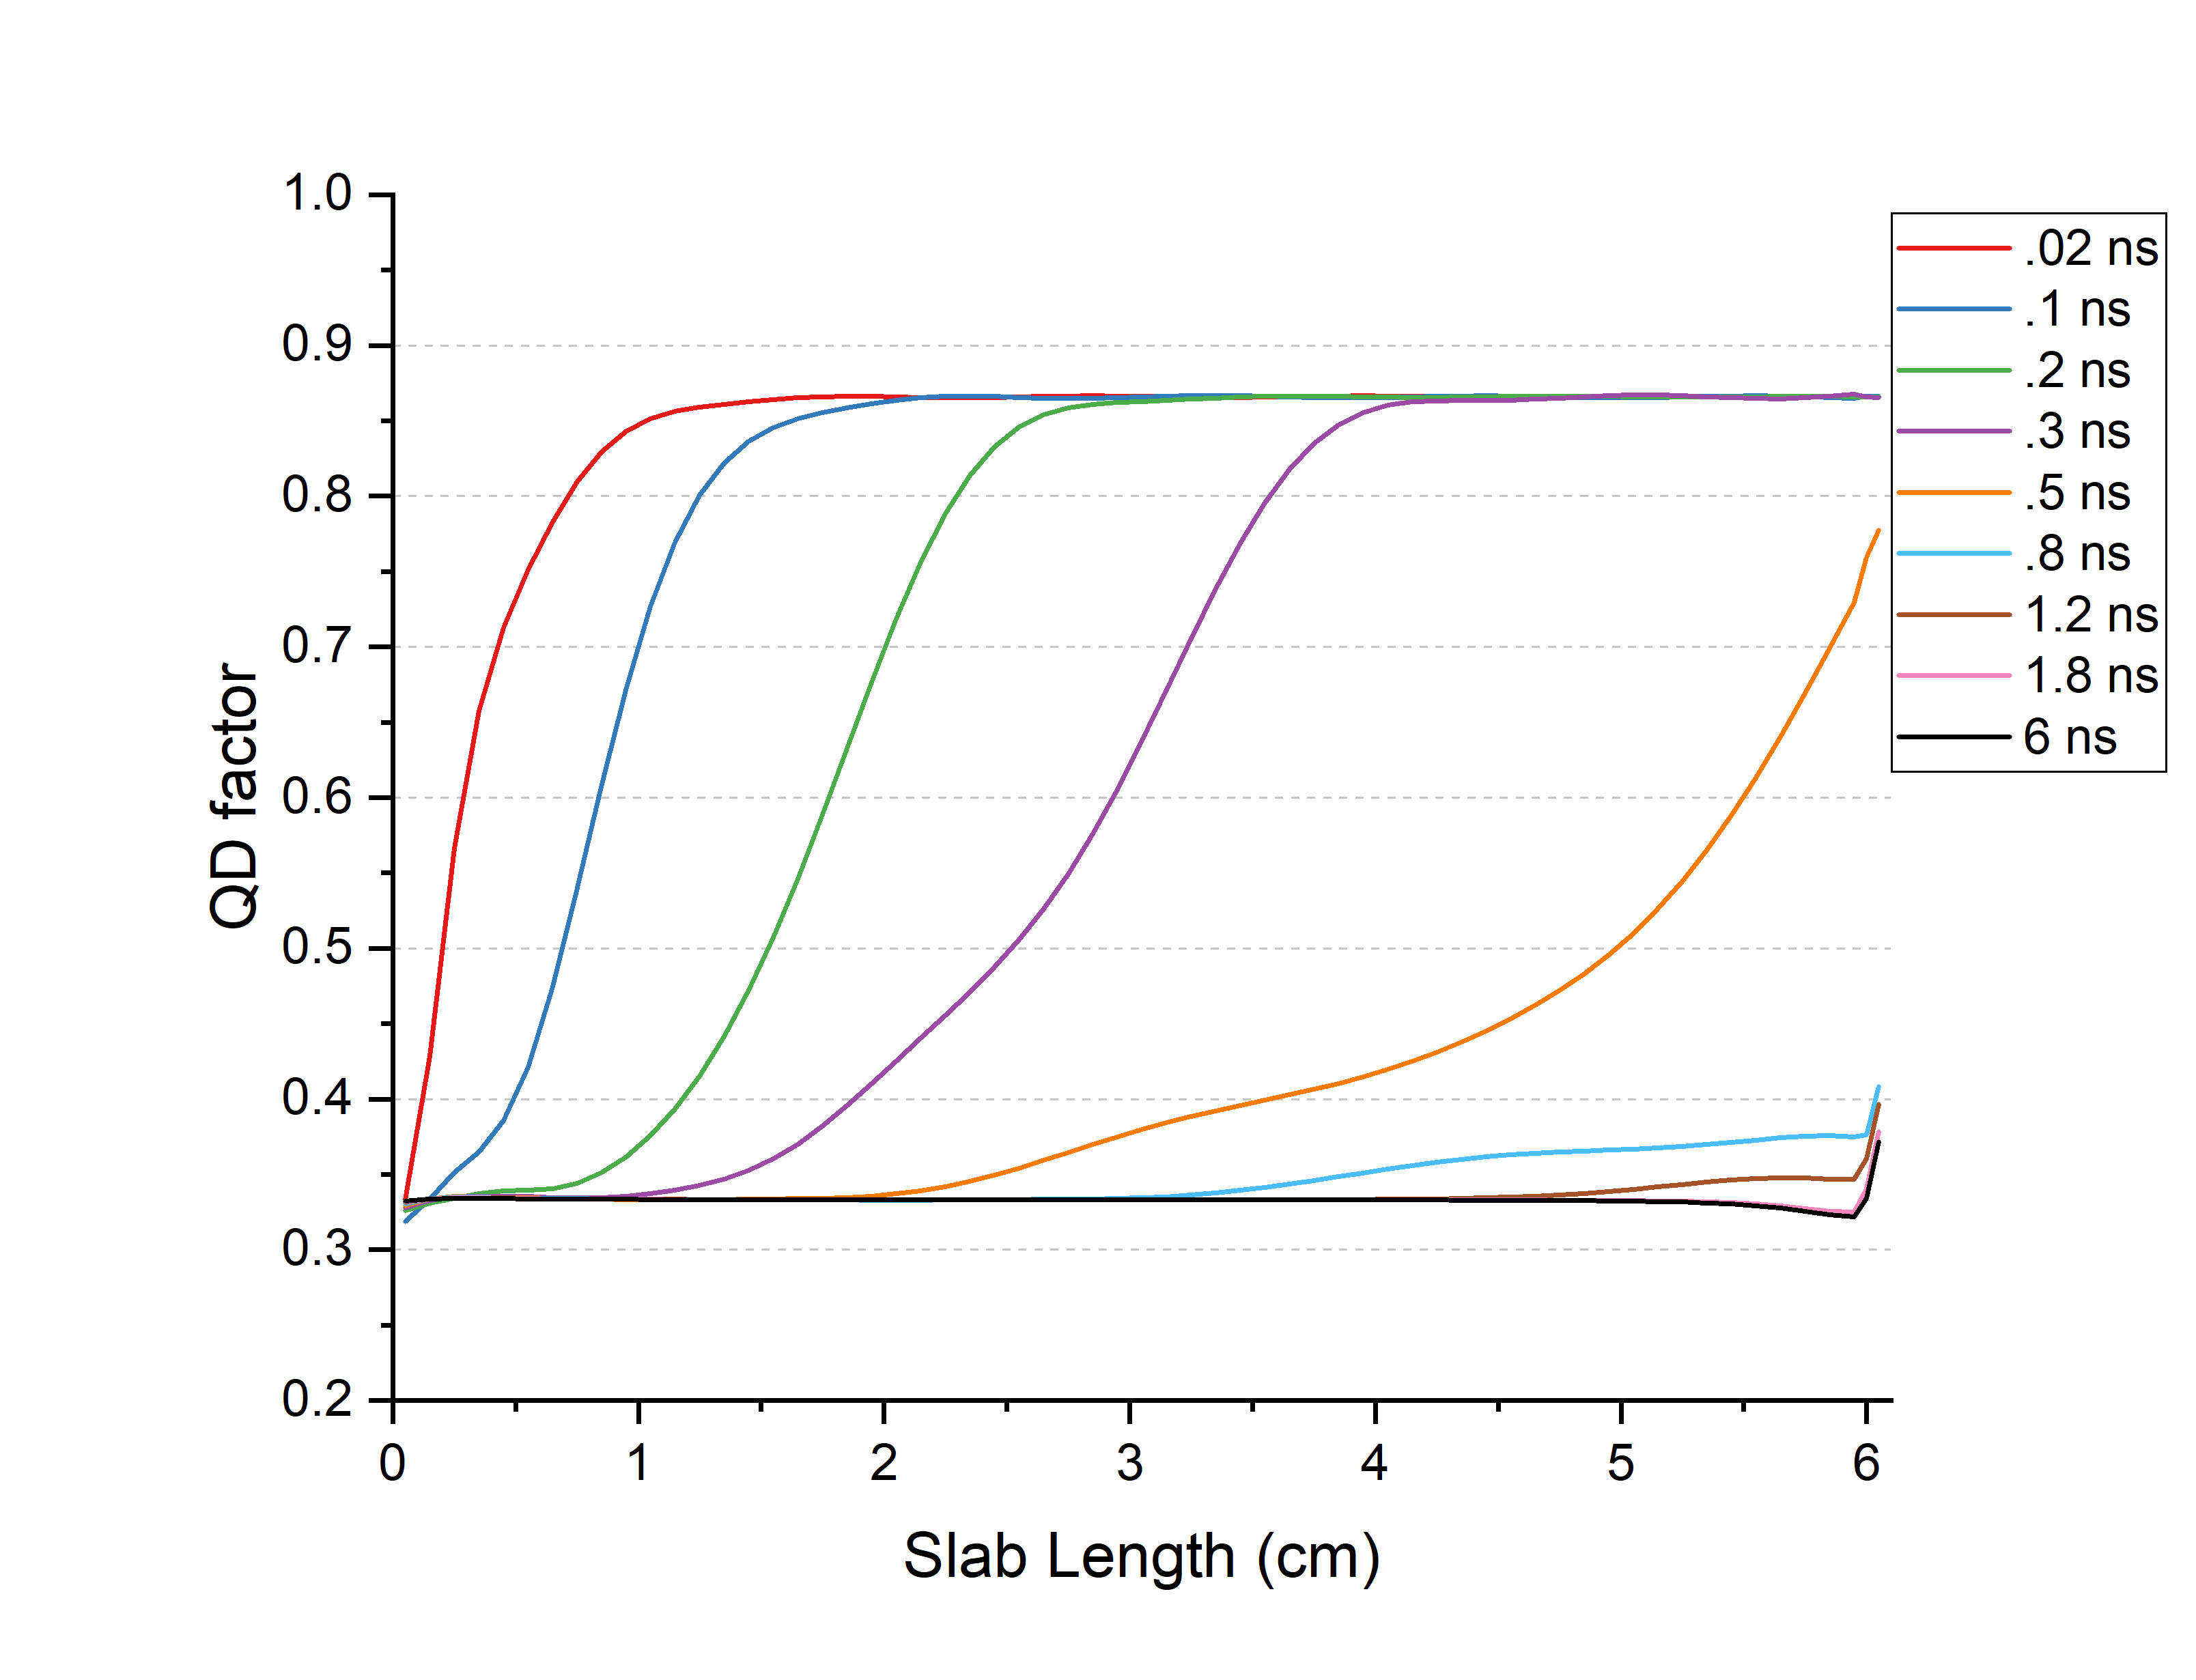
\includegraphics[width=0.5\textwidth]{qdf_g3_cut15.png}}
		\subfloat[r = 20 \label{subfig:qdf_g3_cut20}]{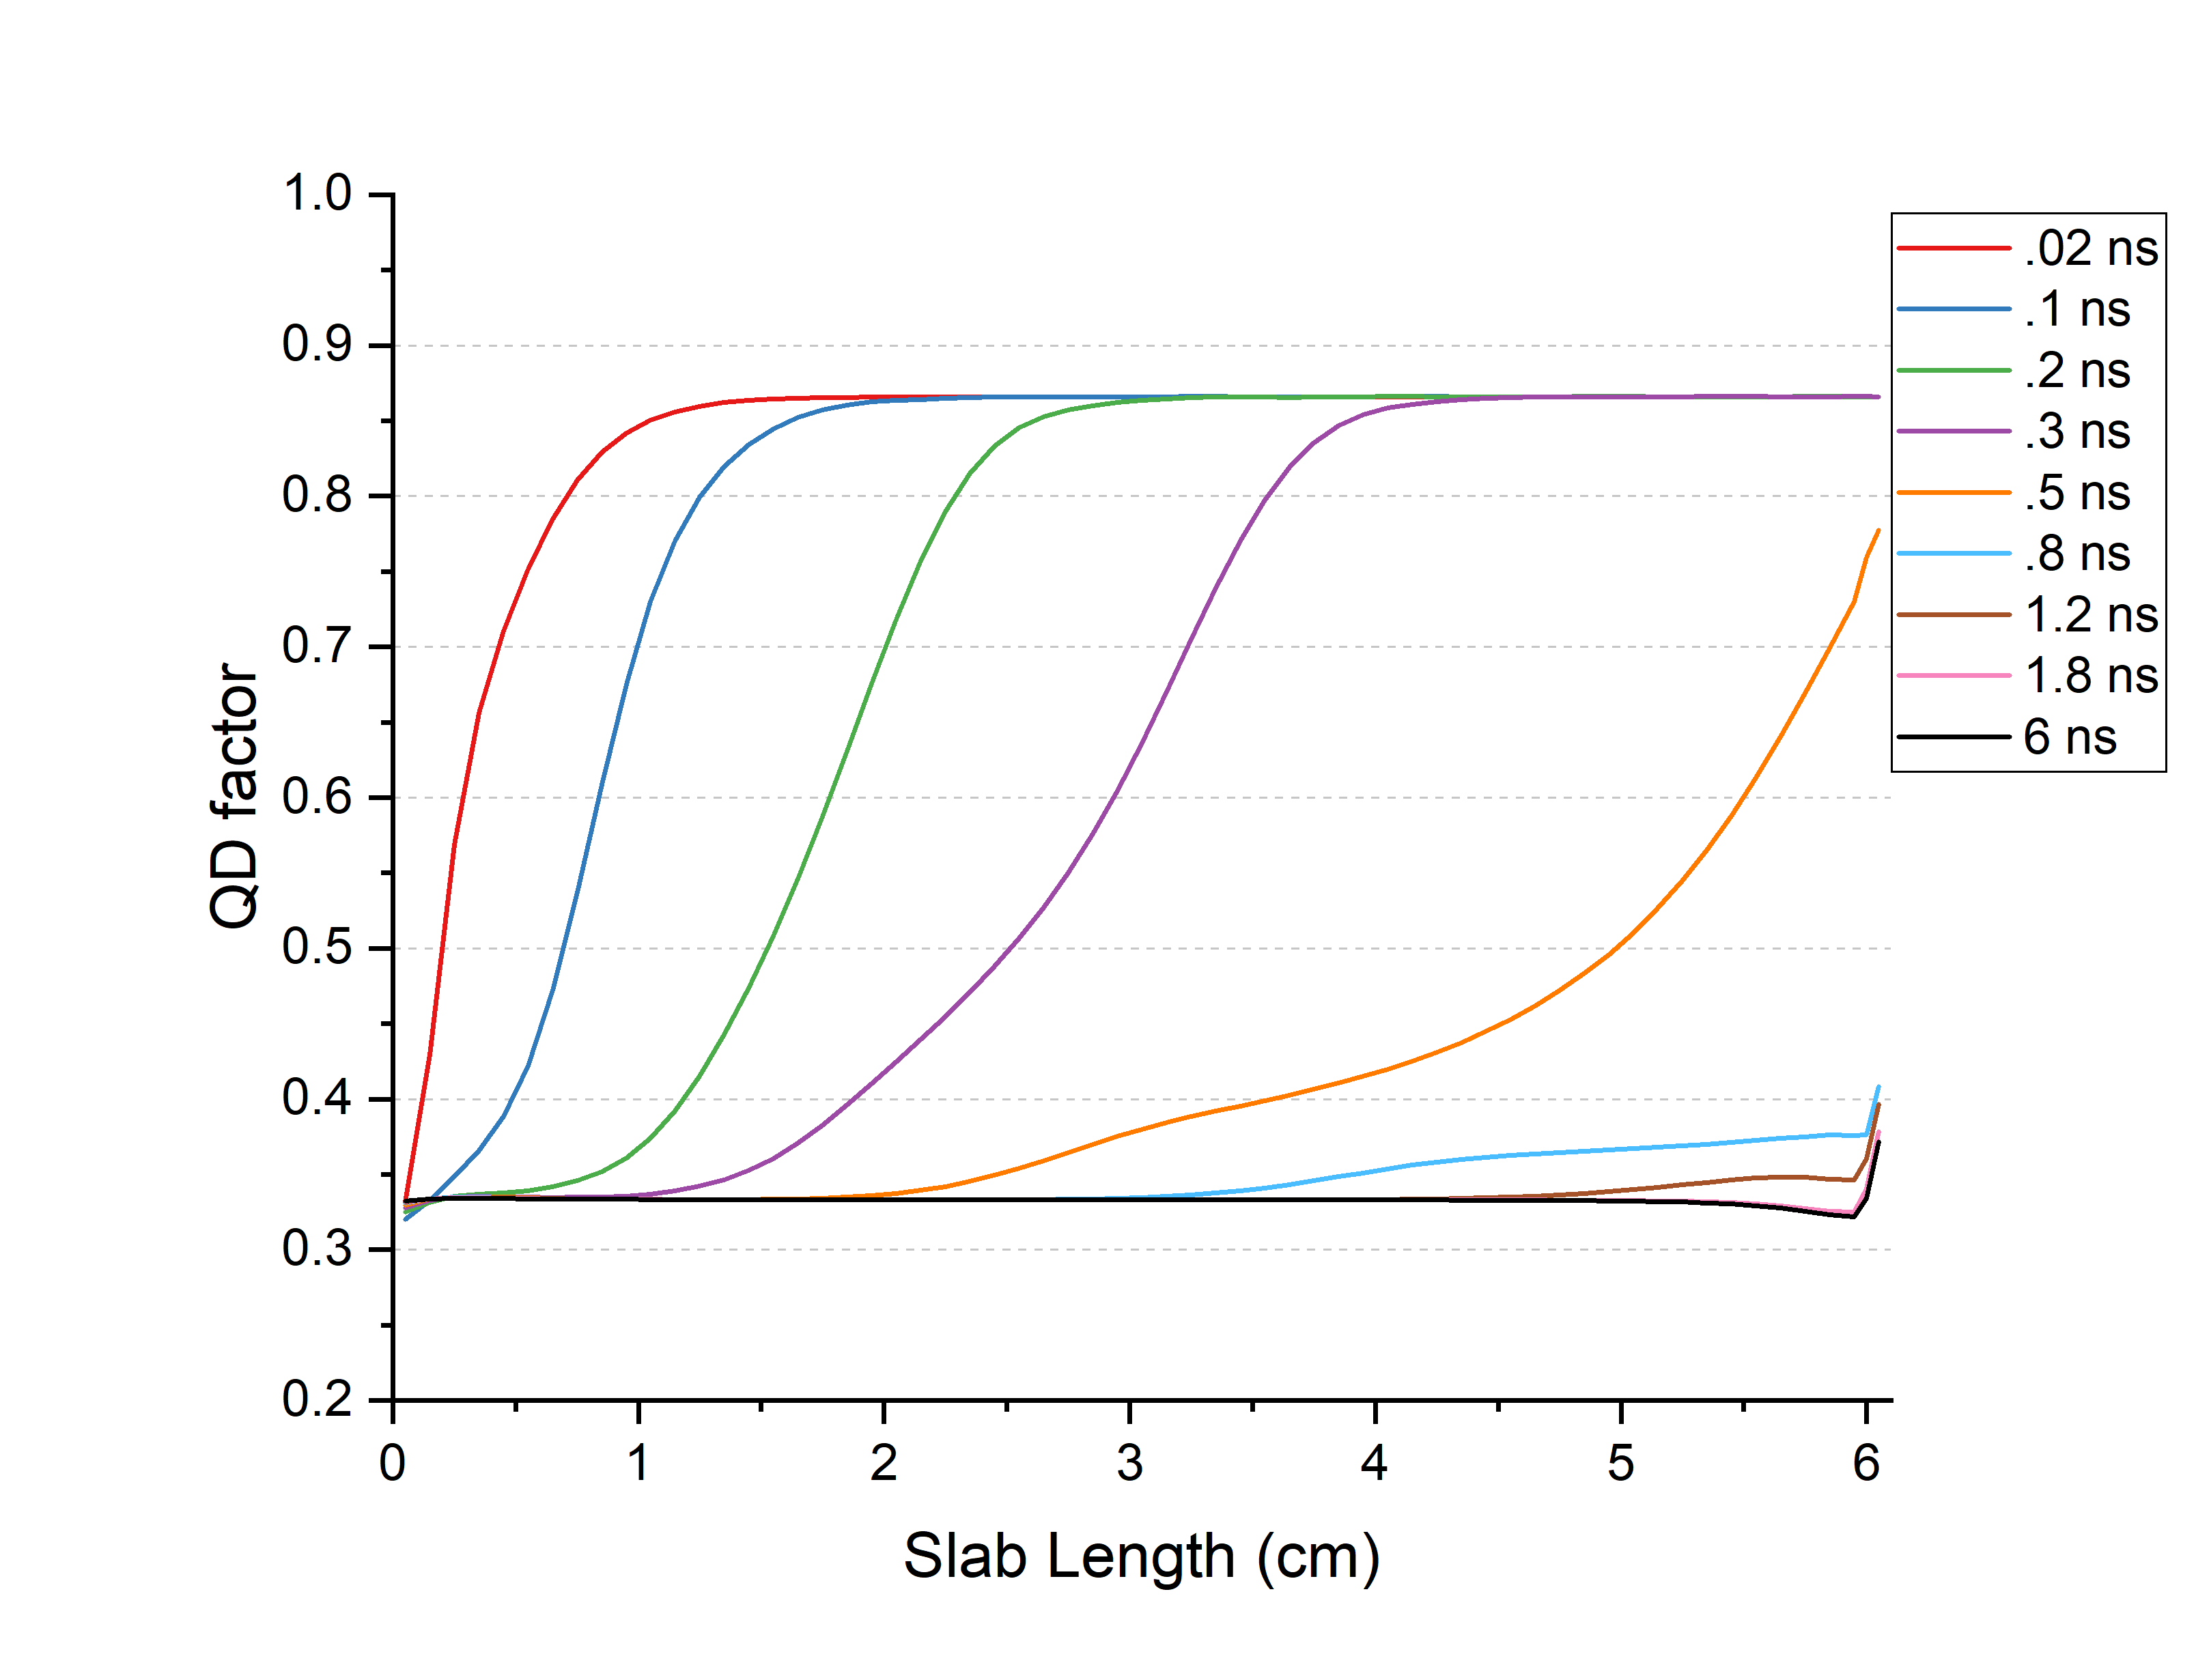
\includegraphics[width=0.5\textwidth]{qdf_g3_cut20.png}}
		\caption{\label{fig:qdf_g3_recomps}
			Low-rank approximation of the group QD factors for $g=3$ for select time steps}
	\end{figure}

	%=================================================================================
	% QDF G8 RECOMP
	\begin{figure}[ht!]
		\centering
		\subfloat[r = 1 \label{subfig:qdf_g8_cut1}]{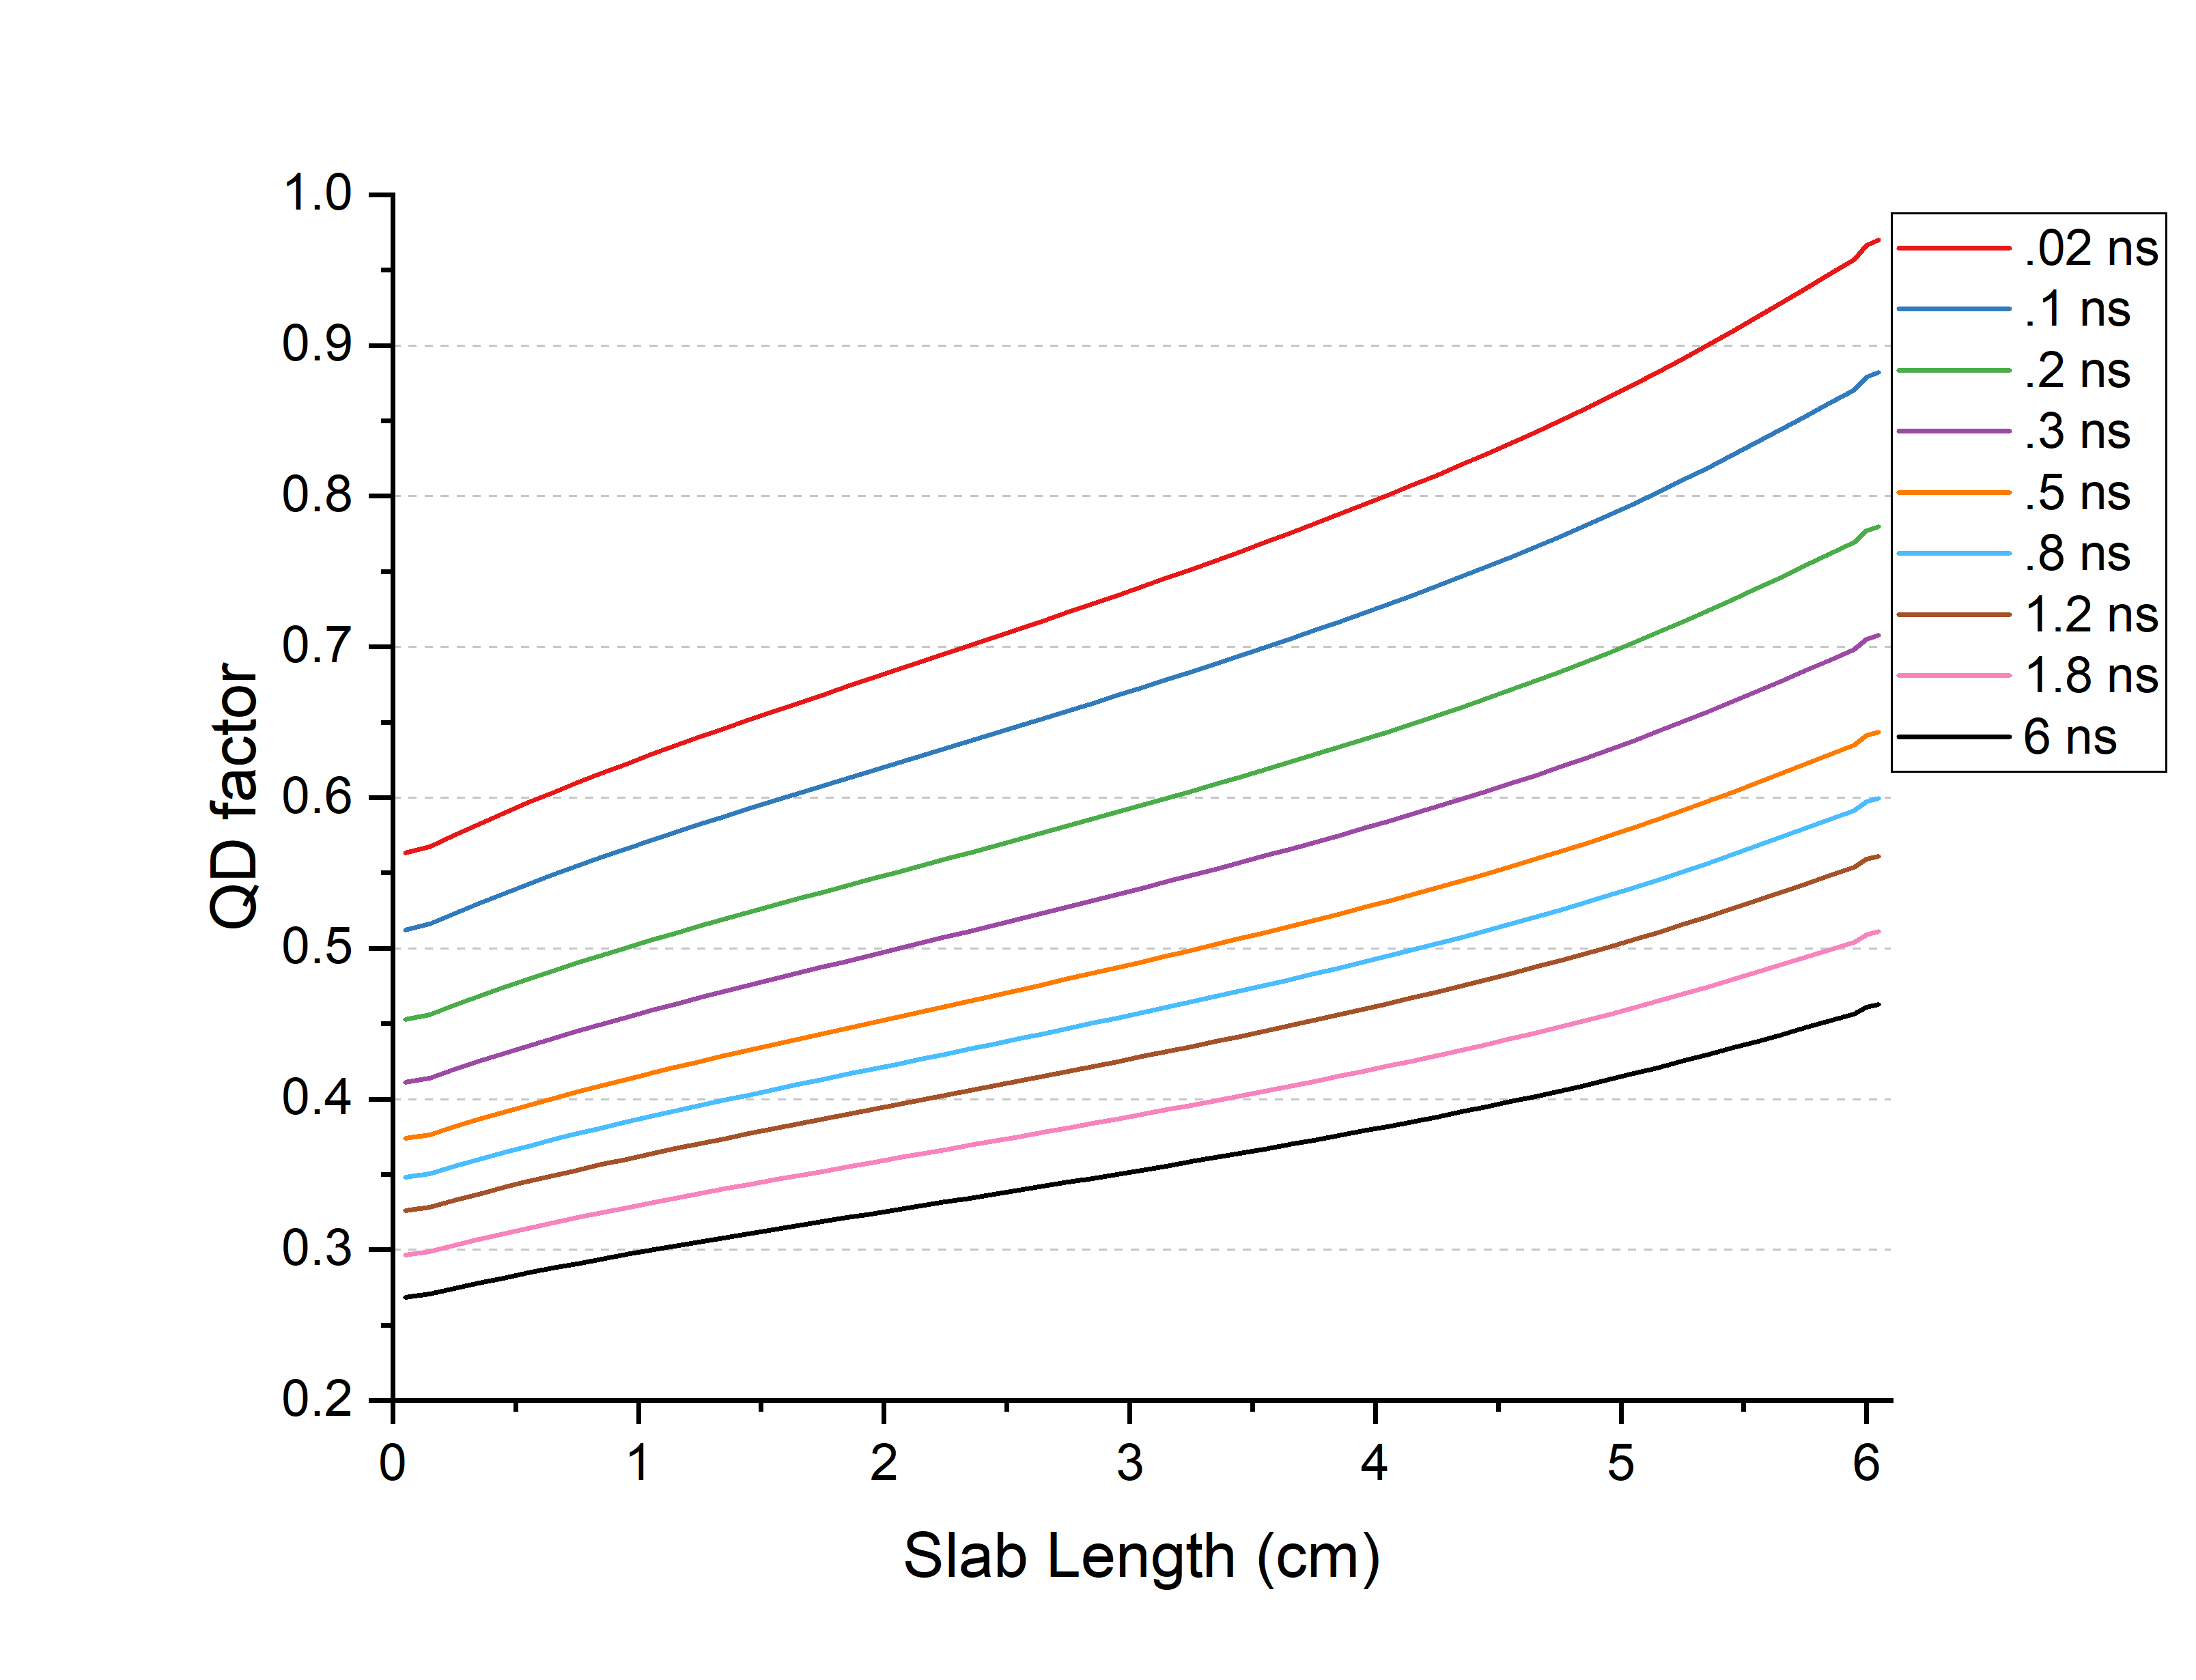
\includegraphics[width=0.5\textwidth]{qdf_g8_cut1.png}}
		\subfloat[r = 2 \label{subfig:qdf_g8_cut2}]{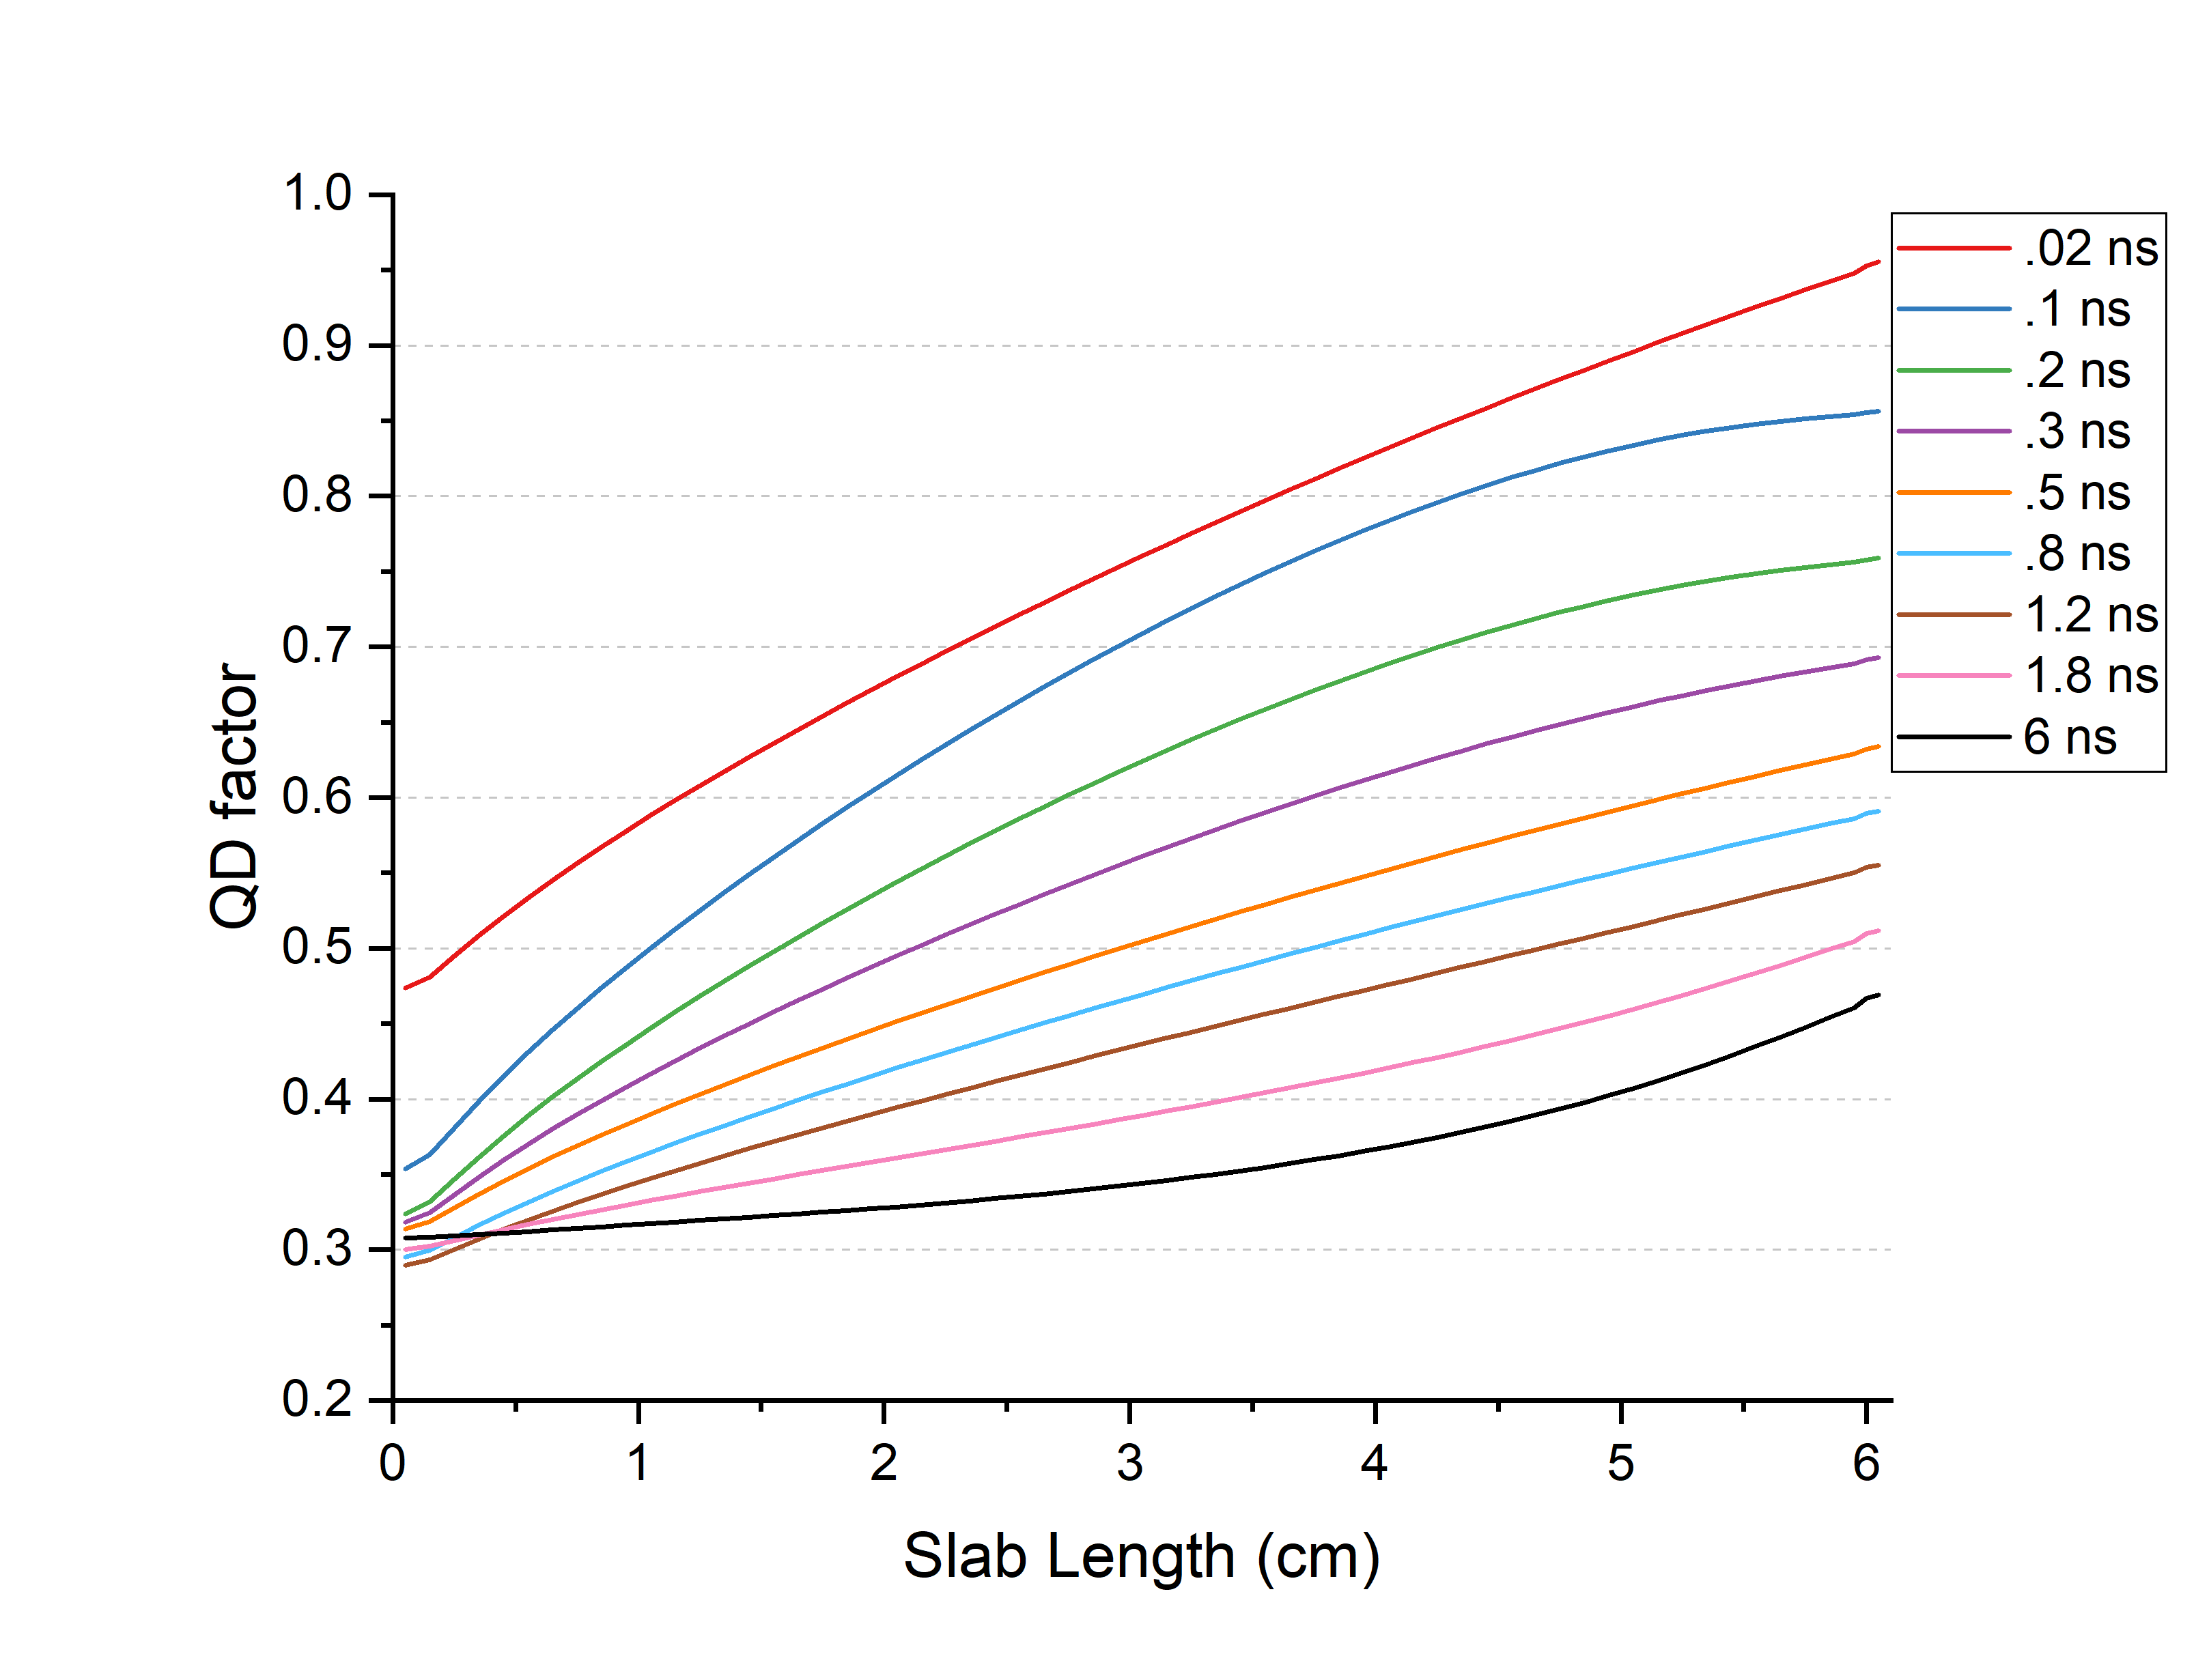
\includegraphics[width=0.5\textwidth]{qdf_g8_cut2.png}}\\
		\subfloat[r = 5 \label{subfig:qdf_g8_cut5}]{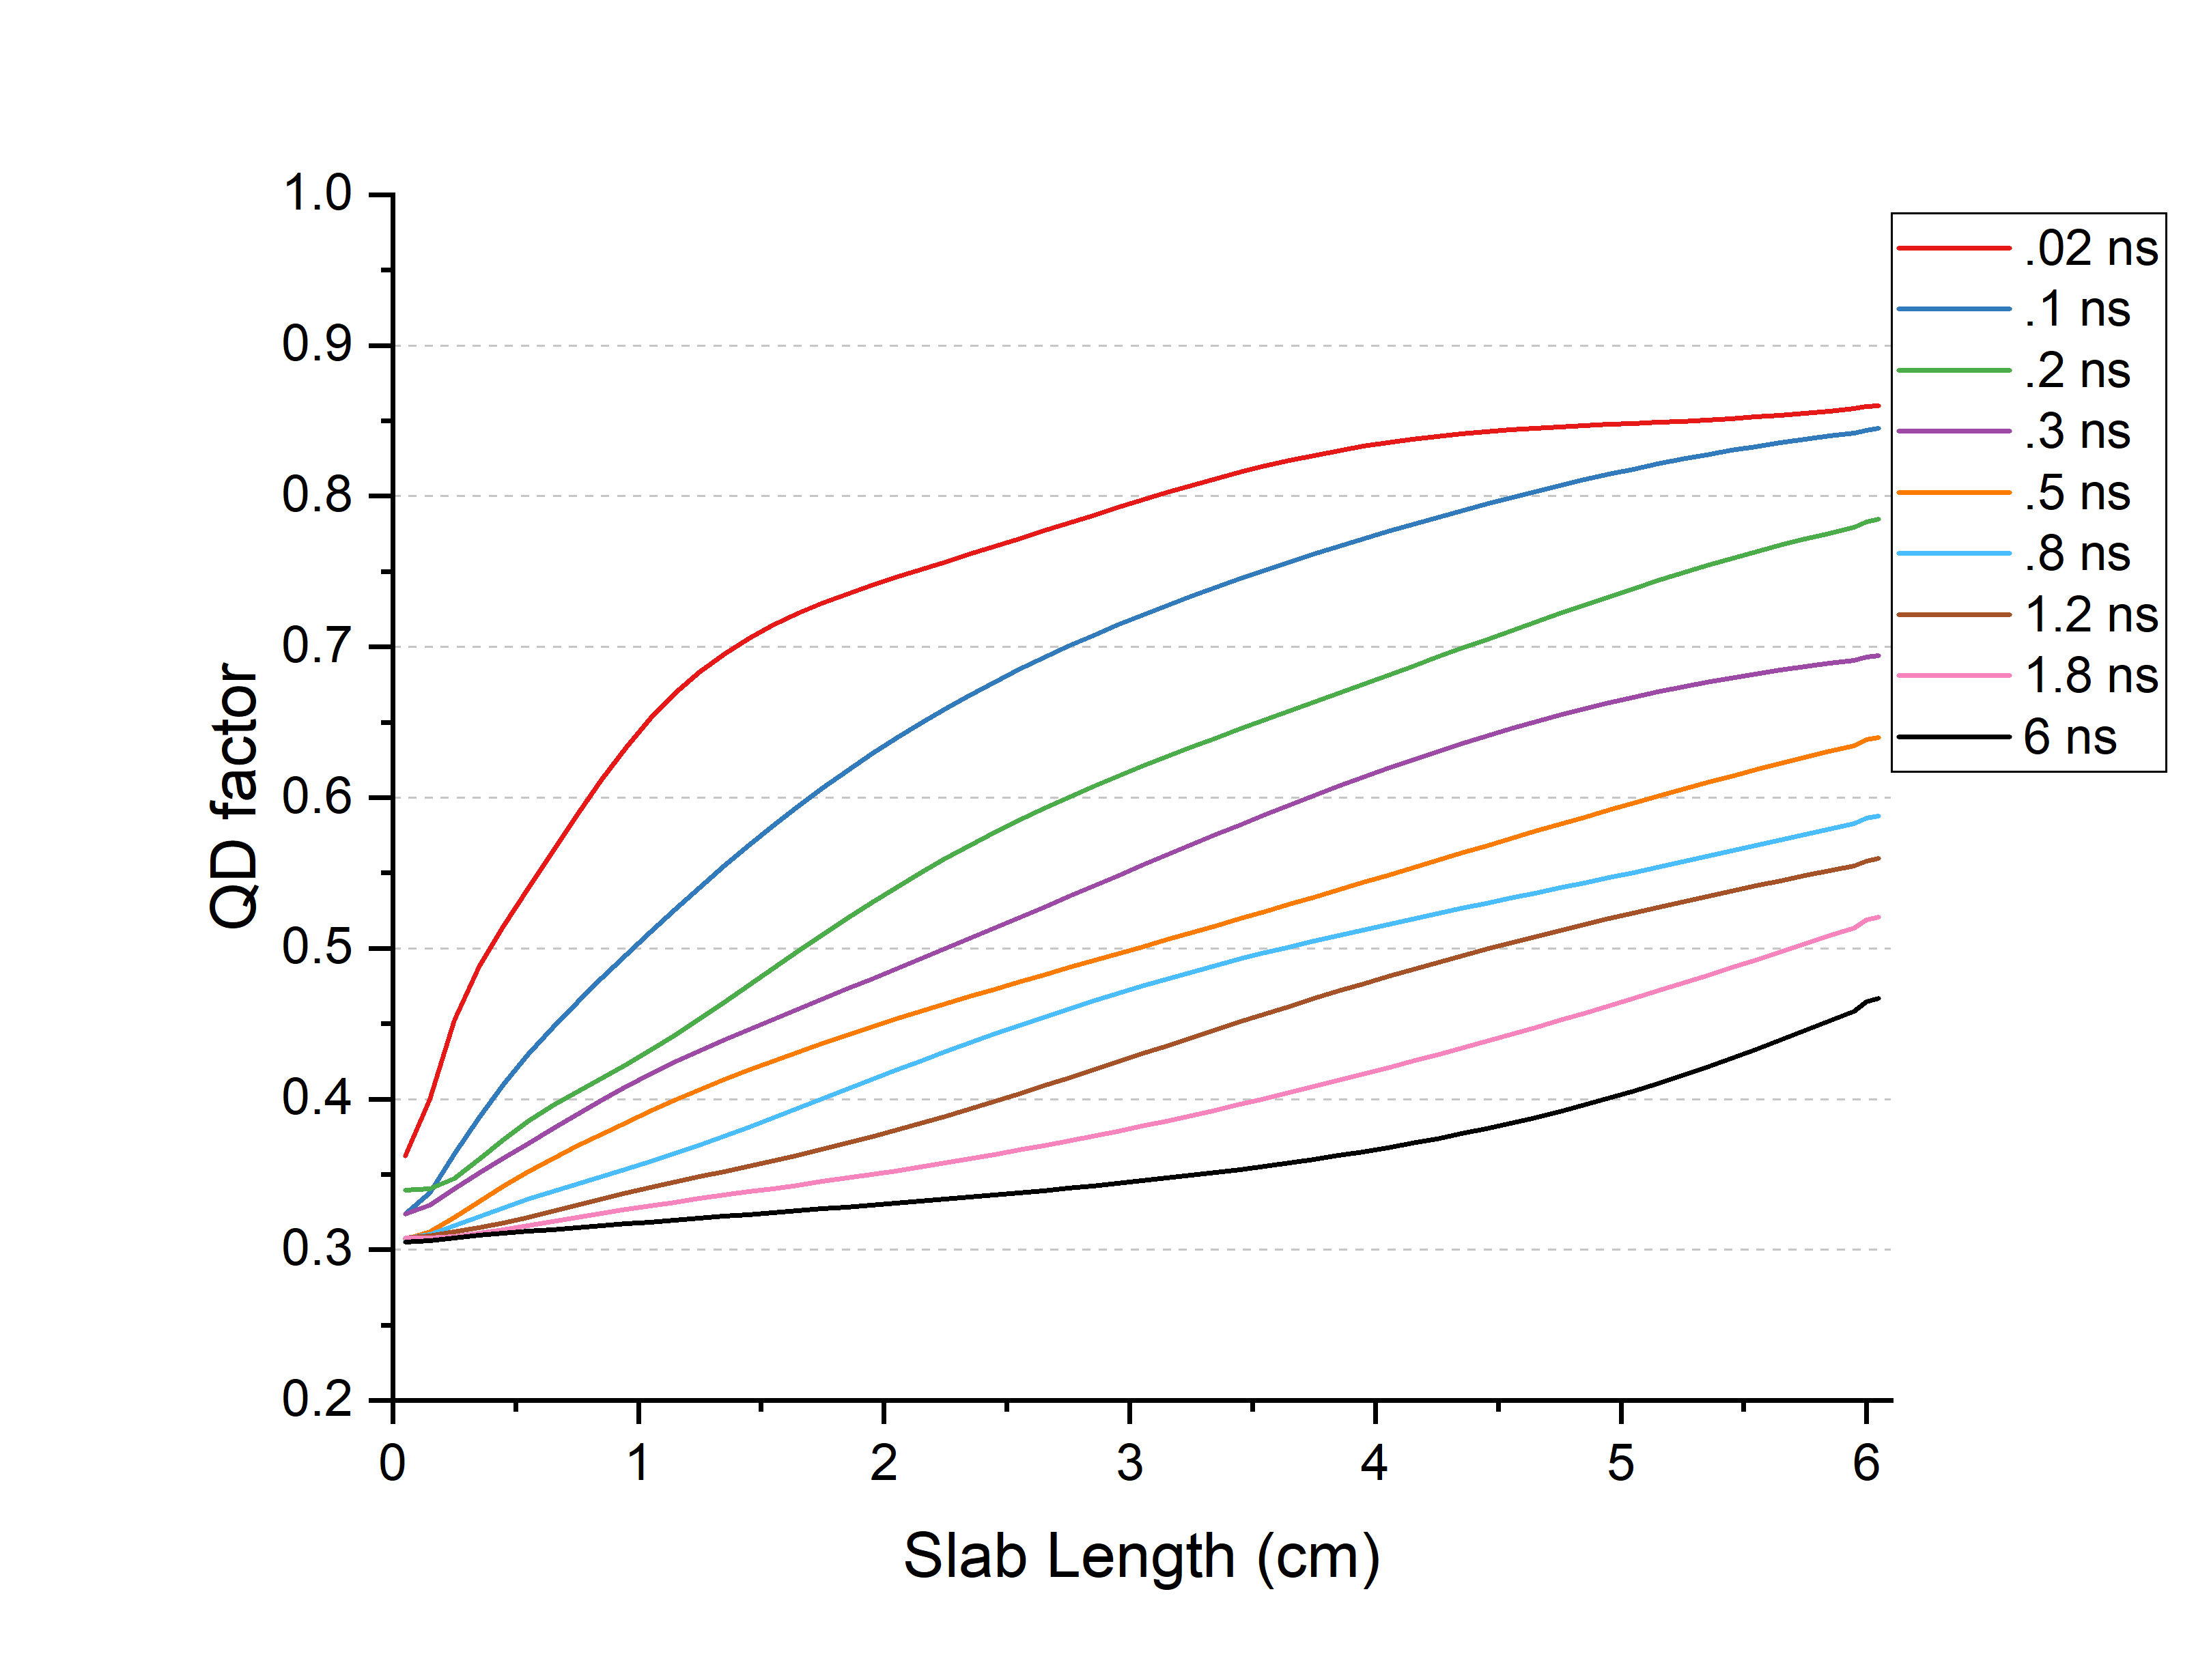
\includegraphics[width=0.5\textwidth]{qdf_g8_cut5.png}}
		\subfloat[r = 10 \label{subfig:qdf_g8_cut10}]{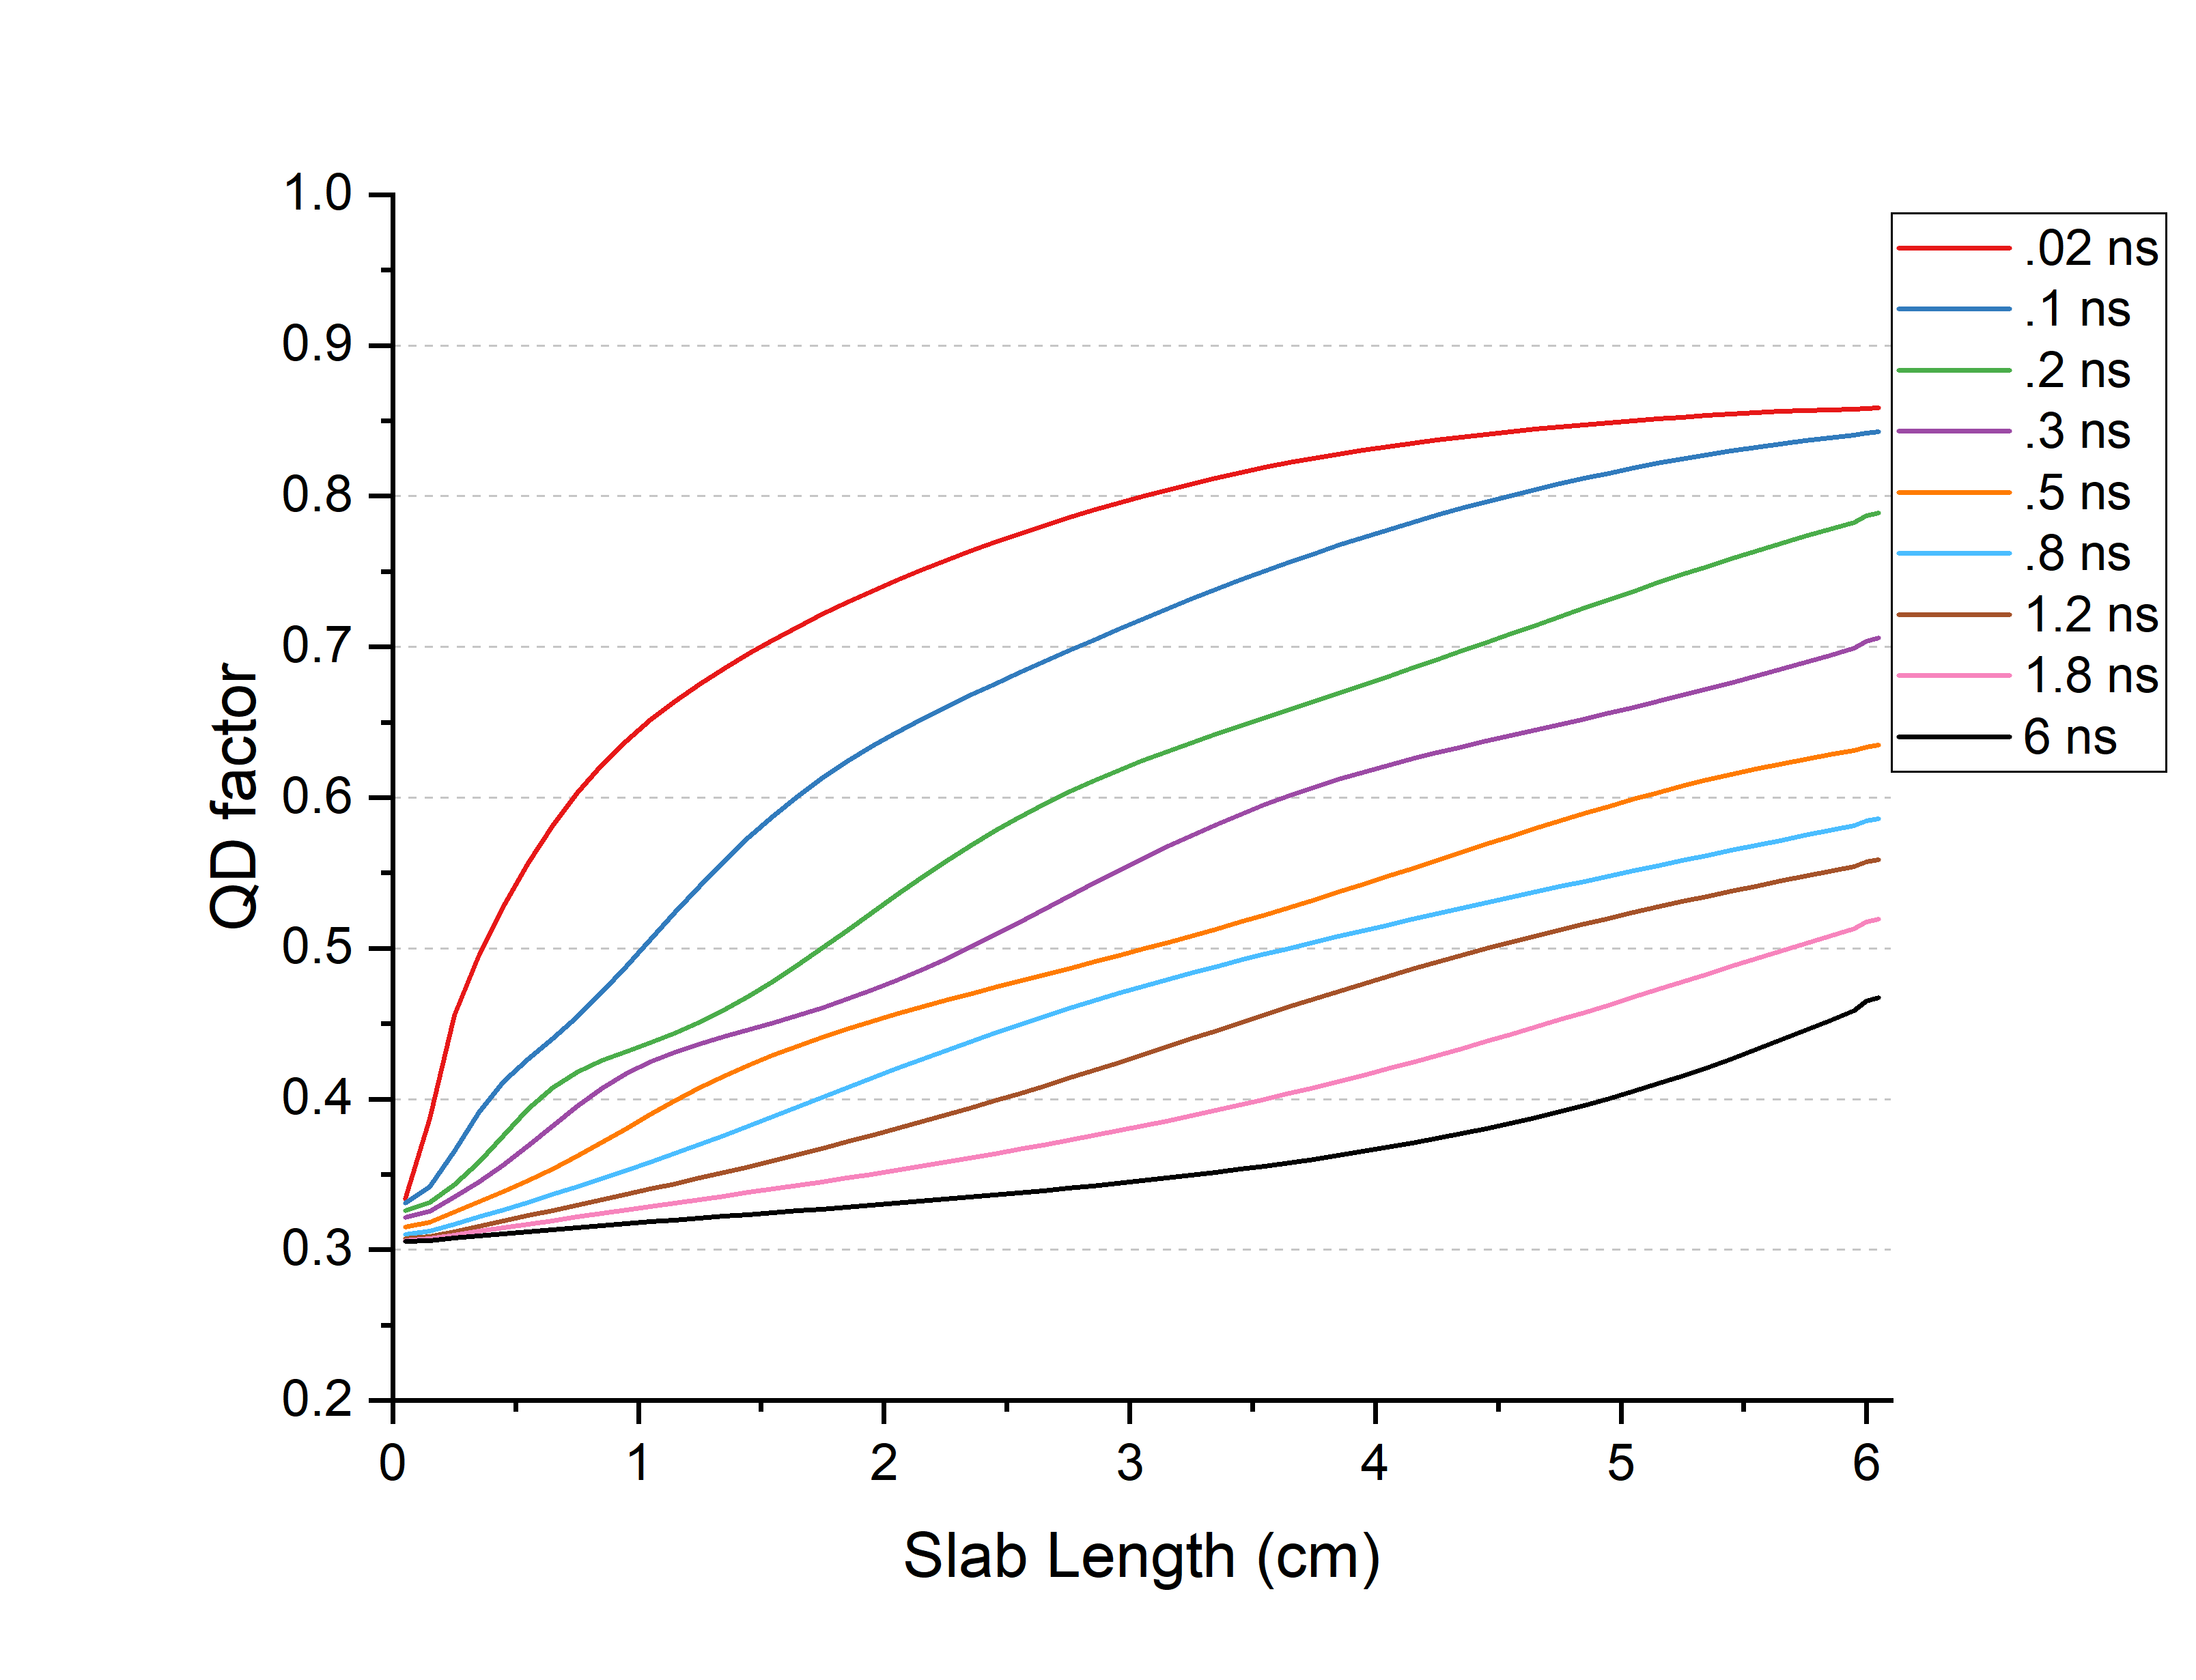
\includegraphics[width=0.5\textwidth]{qdf_g8_cut10.png}}\\
		\subfloat[r = 15 \label{subfig:qdf_g8_cut15}]{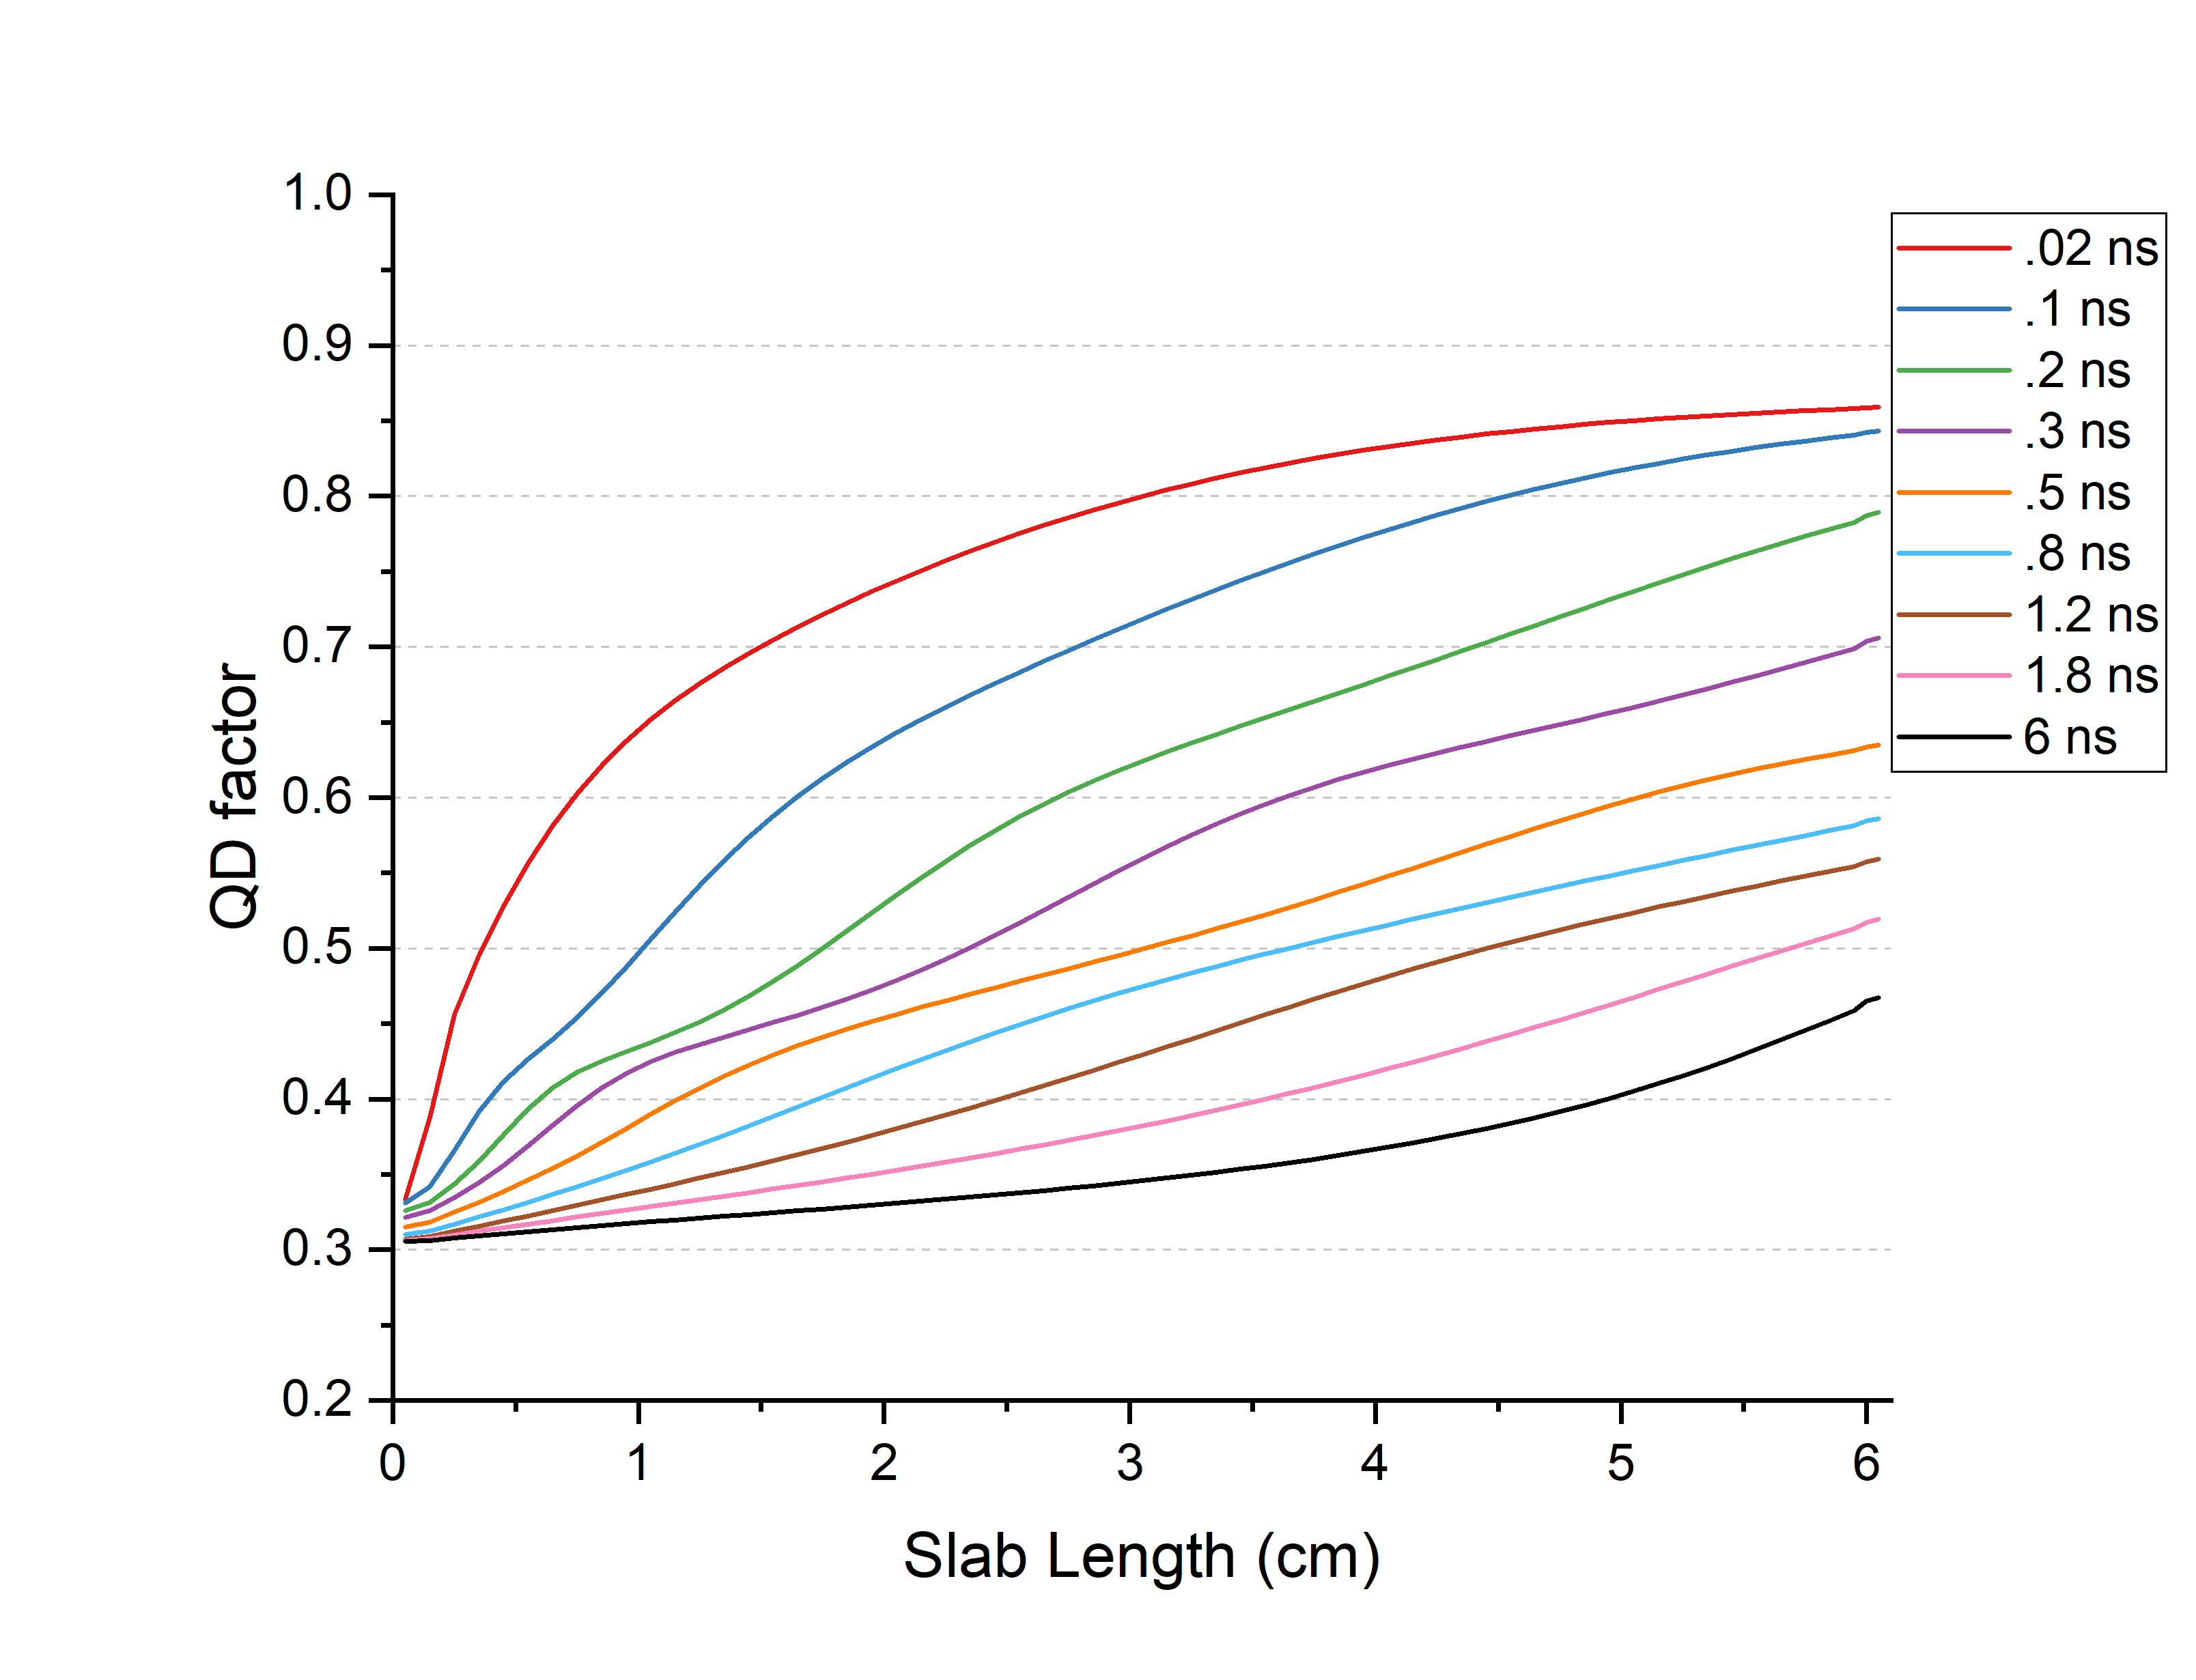
\includegraphics[width=0.5\textwidth]{qdf_g8_cut15.png}}
		\subfloat[r = 20 \label{subfig:qdf_g8_cut20}]{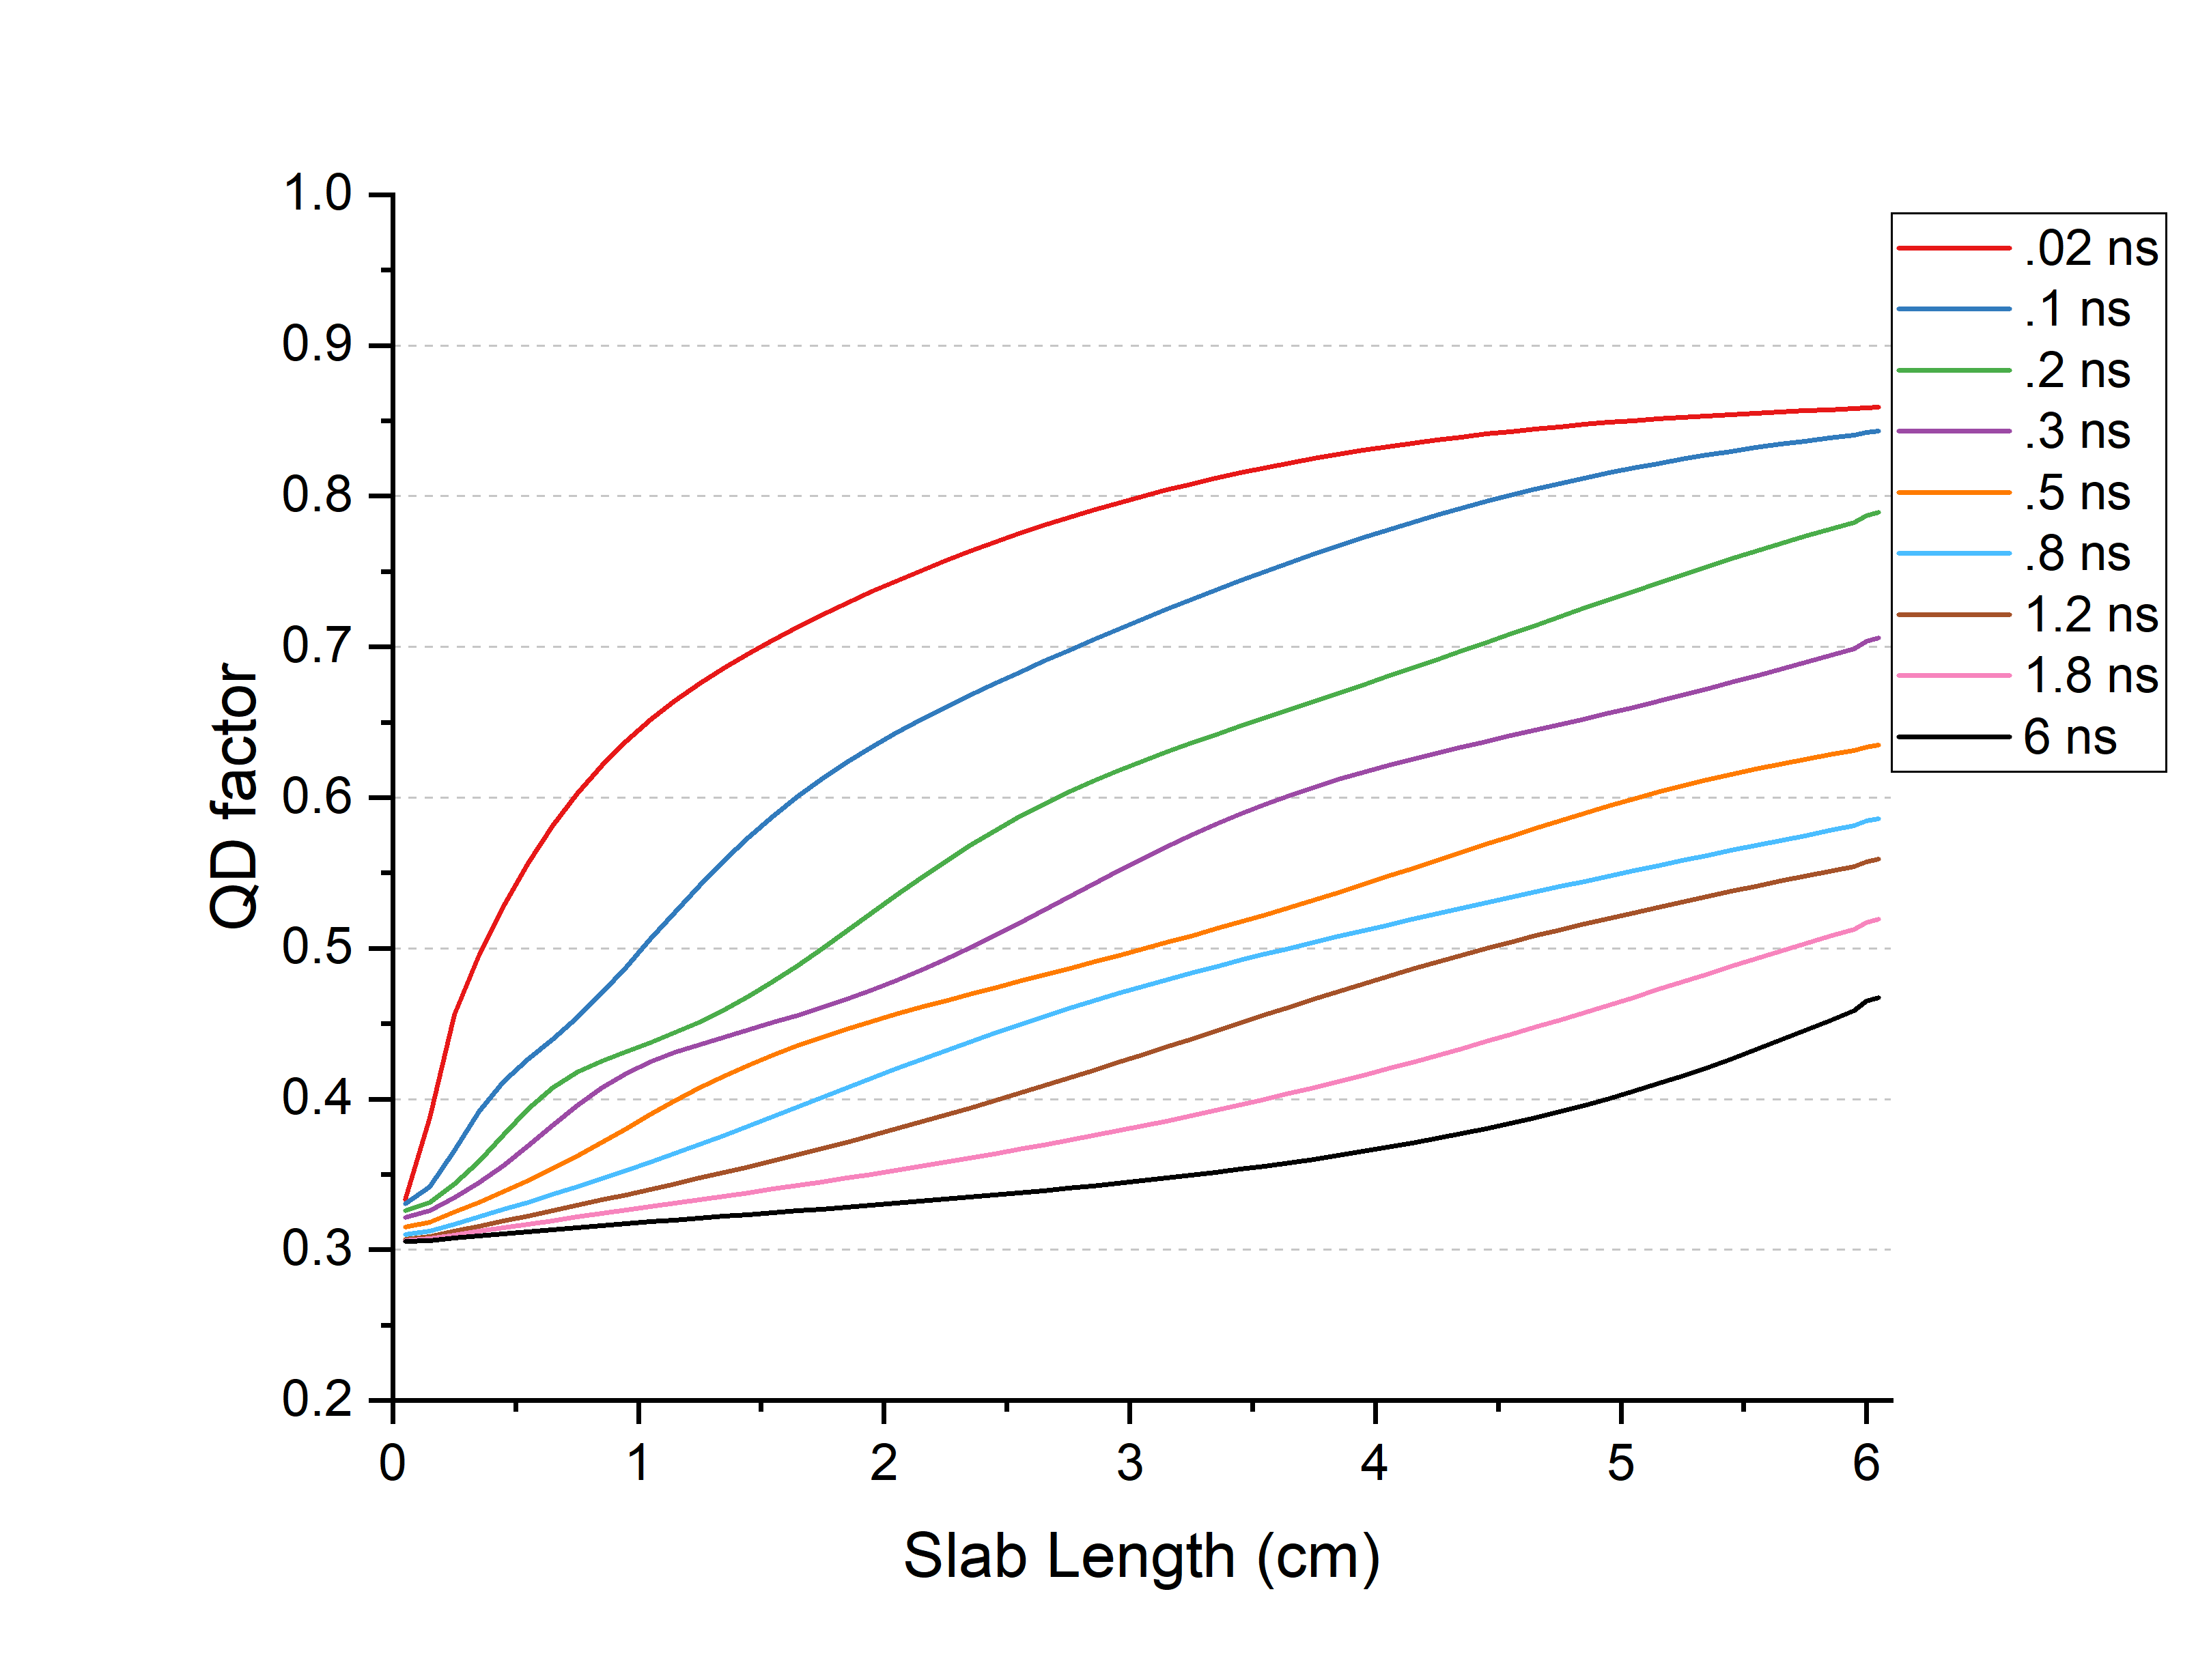
\includegraphics[width=0.5\textwidth]{qdf_g8_cut20.png}}
		\caption{\label{fig:qdf_g8_recomps}
			Low-rank approximation of the group QD factors for $g=8$ for select time steps}
	\end{figure}

\section{Numerical Results of the MLOQD-POD ROM} \label{sec:mloqd-pod_res}
	\ind The F-C test (Sec. \ref{sec:mpod_test}) is solved with the MLOQD-POD ROM for $0 \le t  \le 6$ ns using  the time step length $\Delta t=2 \times 10^{-2}$ ns. Thus, there are 300 time steps. This is the number of snapshots used to build the data set of reference QD factors. We consider MLOQD-POD ROMs using singular value relative cutoff criteria of $\varepsilon_\sigma = 10^{-1}, 10^{-2}, \dots 10^{-12}$. Figure \ref{fig:ref_errs_inf} presents the relative error of the solution of these MLOQD-POD ROMs compared to the  reference solution in the  $\infty$-norm at every instant of time. The results show how the accuracy of MLOQD-POD ROMs improves as $\varepsilon_\sigma$  decreases. The relative error is decreases in magnitude at every instant of time for both temperature and energy density for each successive decrease of $\varepsilon_\sigma$. Note that  both temperature and energy density obtained by means of these MLOQD-POQ ROMs eventually match the reference solution, as the relative error reaches the level of convergence specified for the test problem $\pr{\epsilon_T=\epsilon_E=10^{-12}}$.

	%=================================================================================
	% TEST PROBLEM ERRORS
	\begin{figure}[ht!]
		\centering
		\subfloat[Temperature relative error \label{subfig:refcase_Temp_rel_inf}]{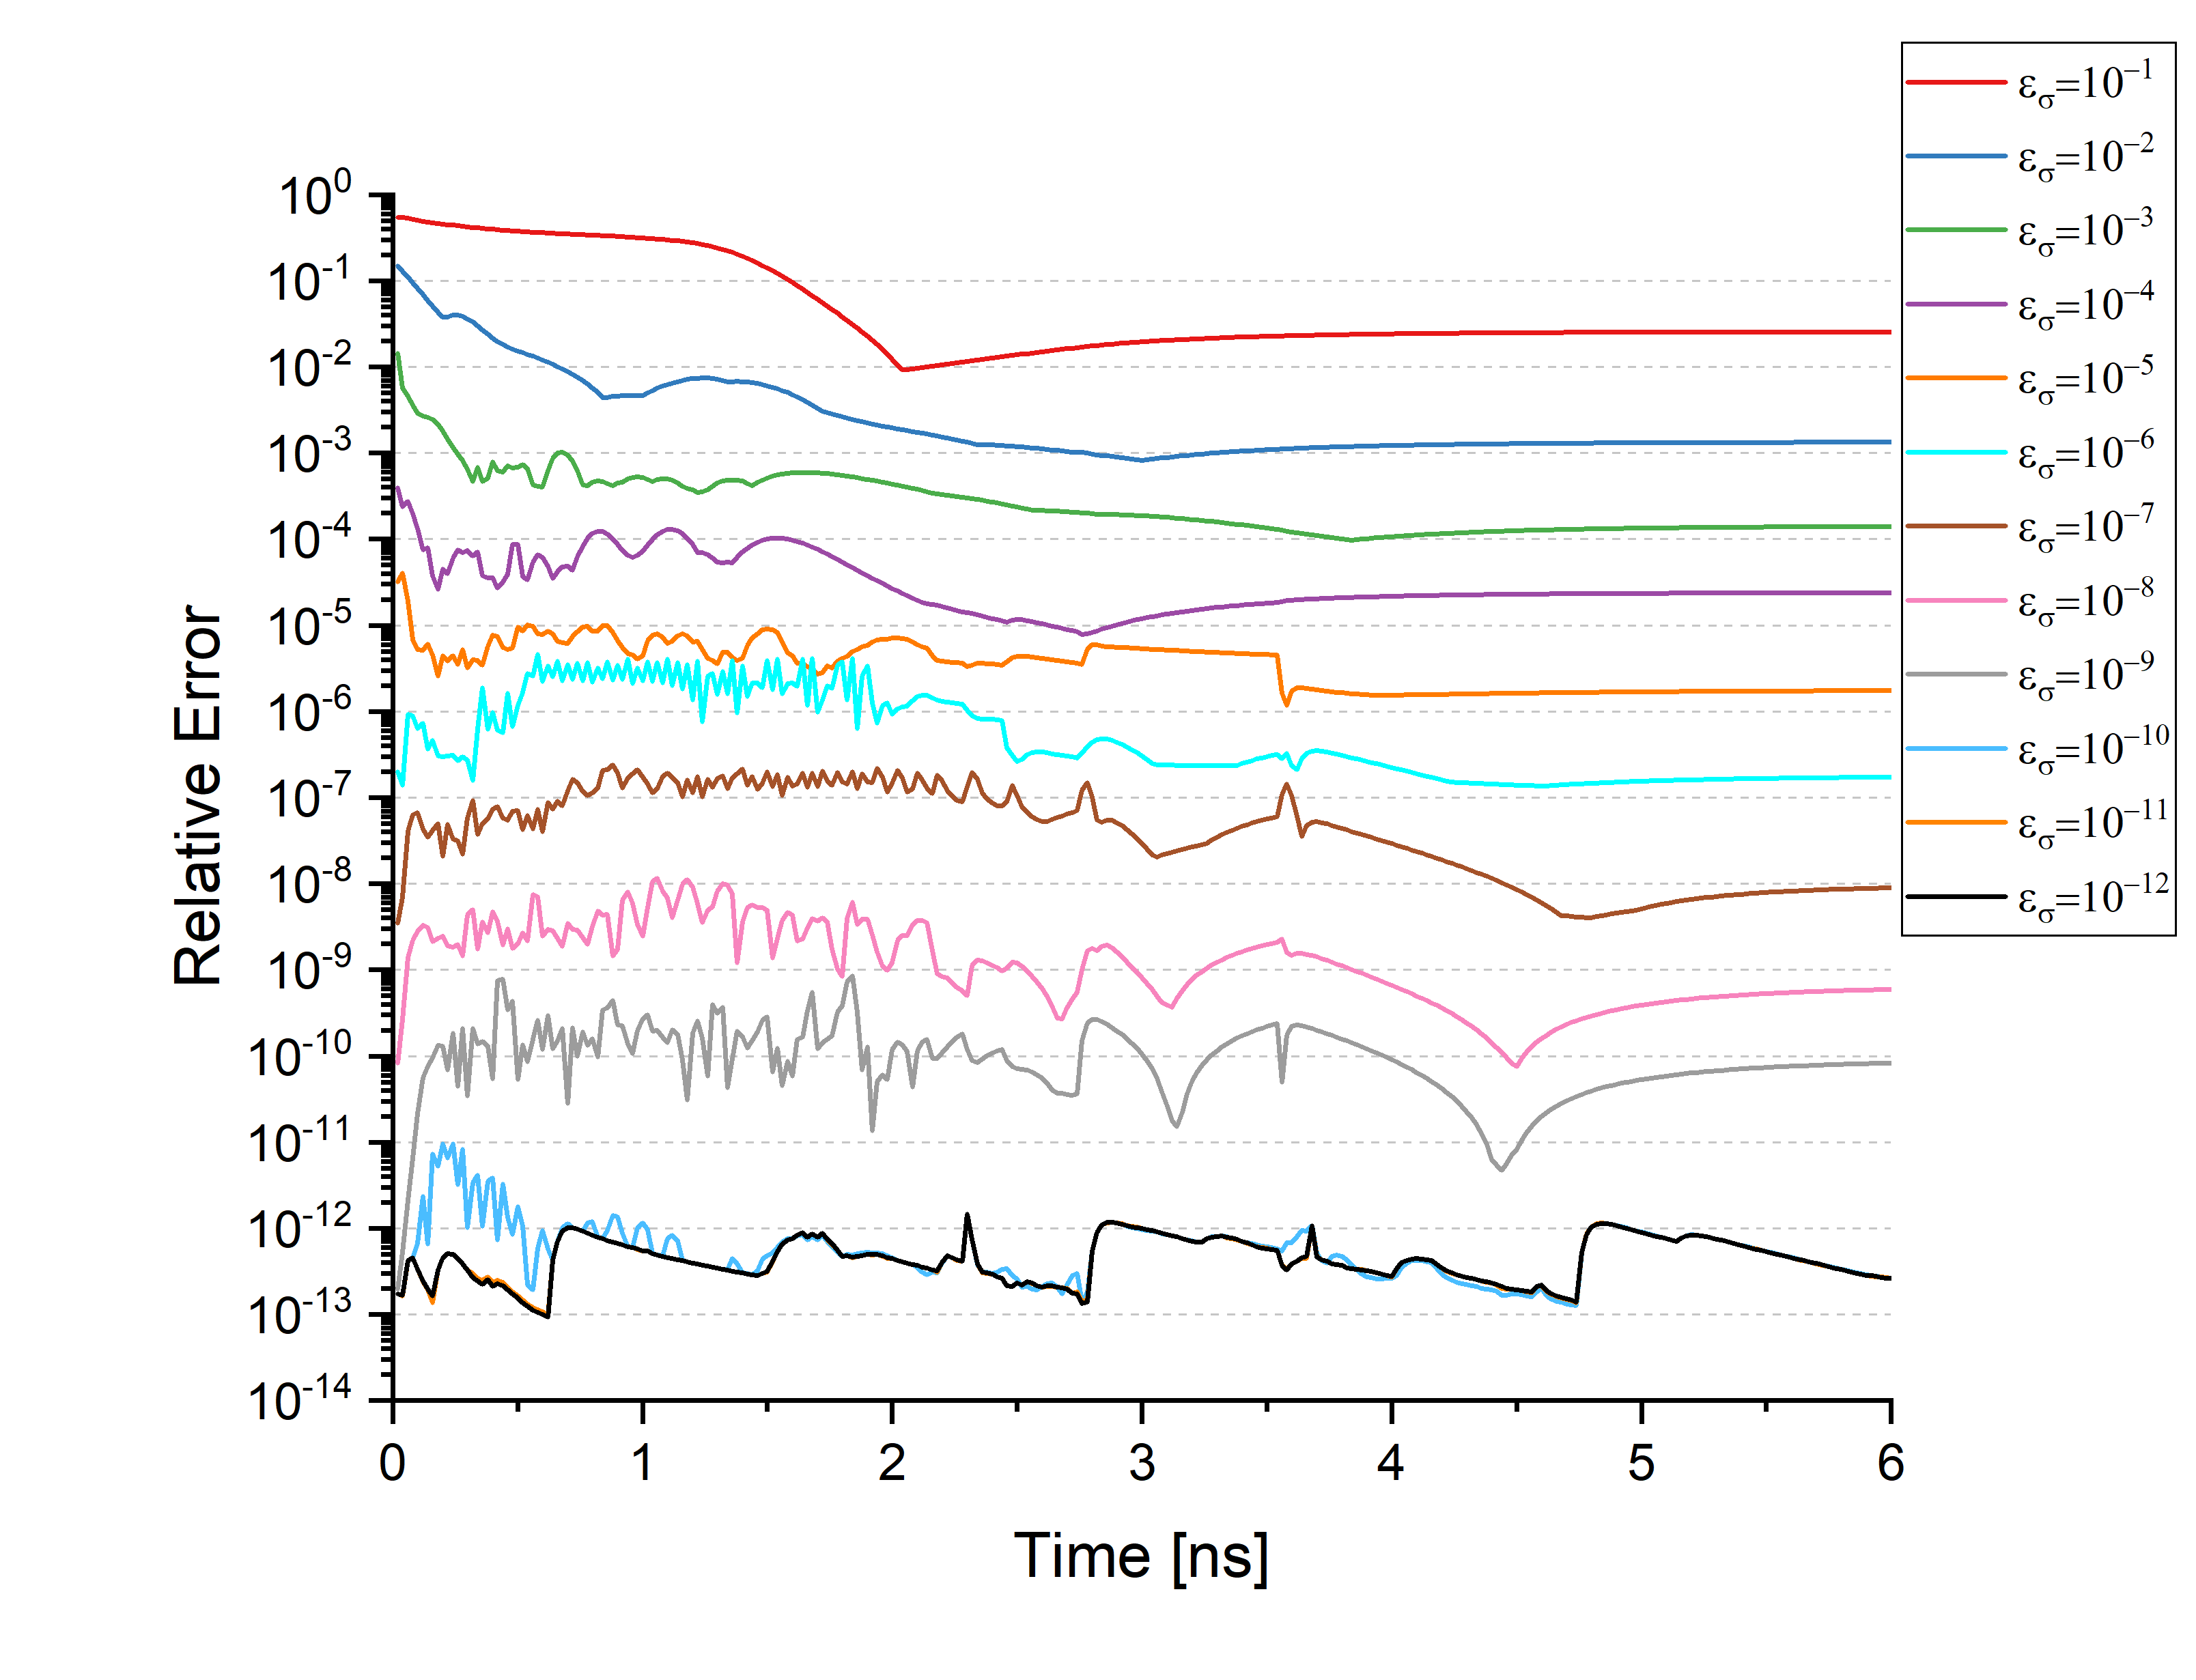
\includegraphics[width=0.5\textwidth]{refcase_Temp_rel_inf.png}}
		\subfloat[Total energy density relative error \label{subfig:refcase_E_rel_inf}]{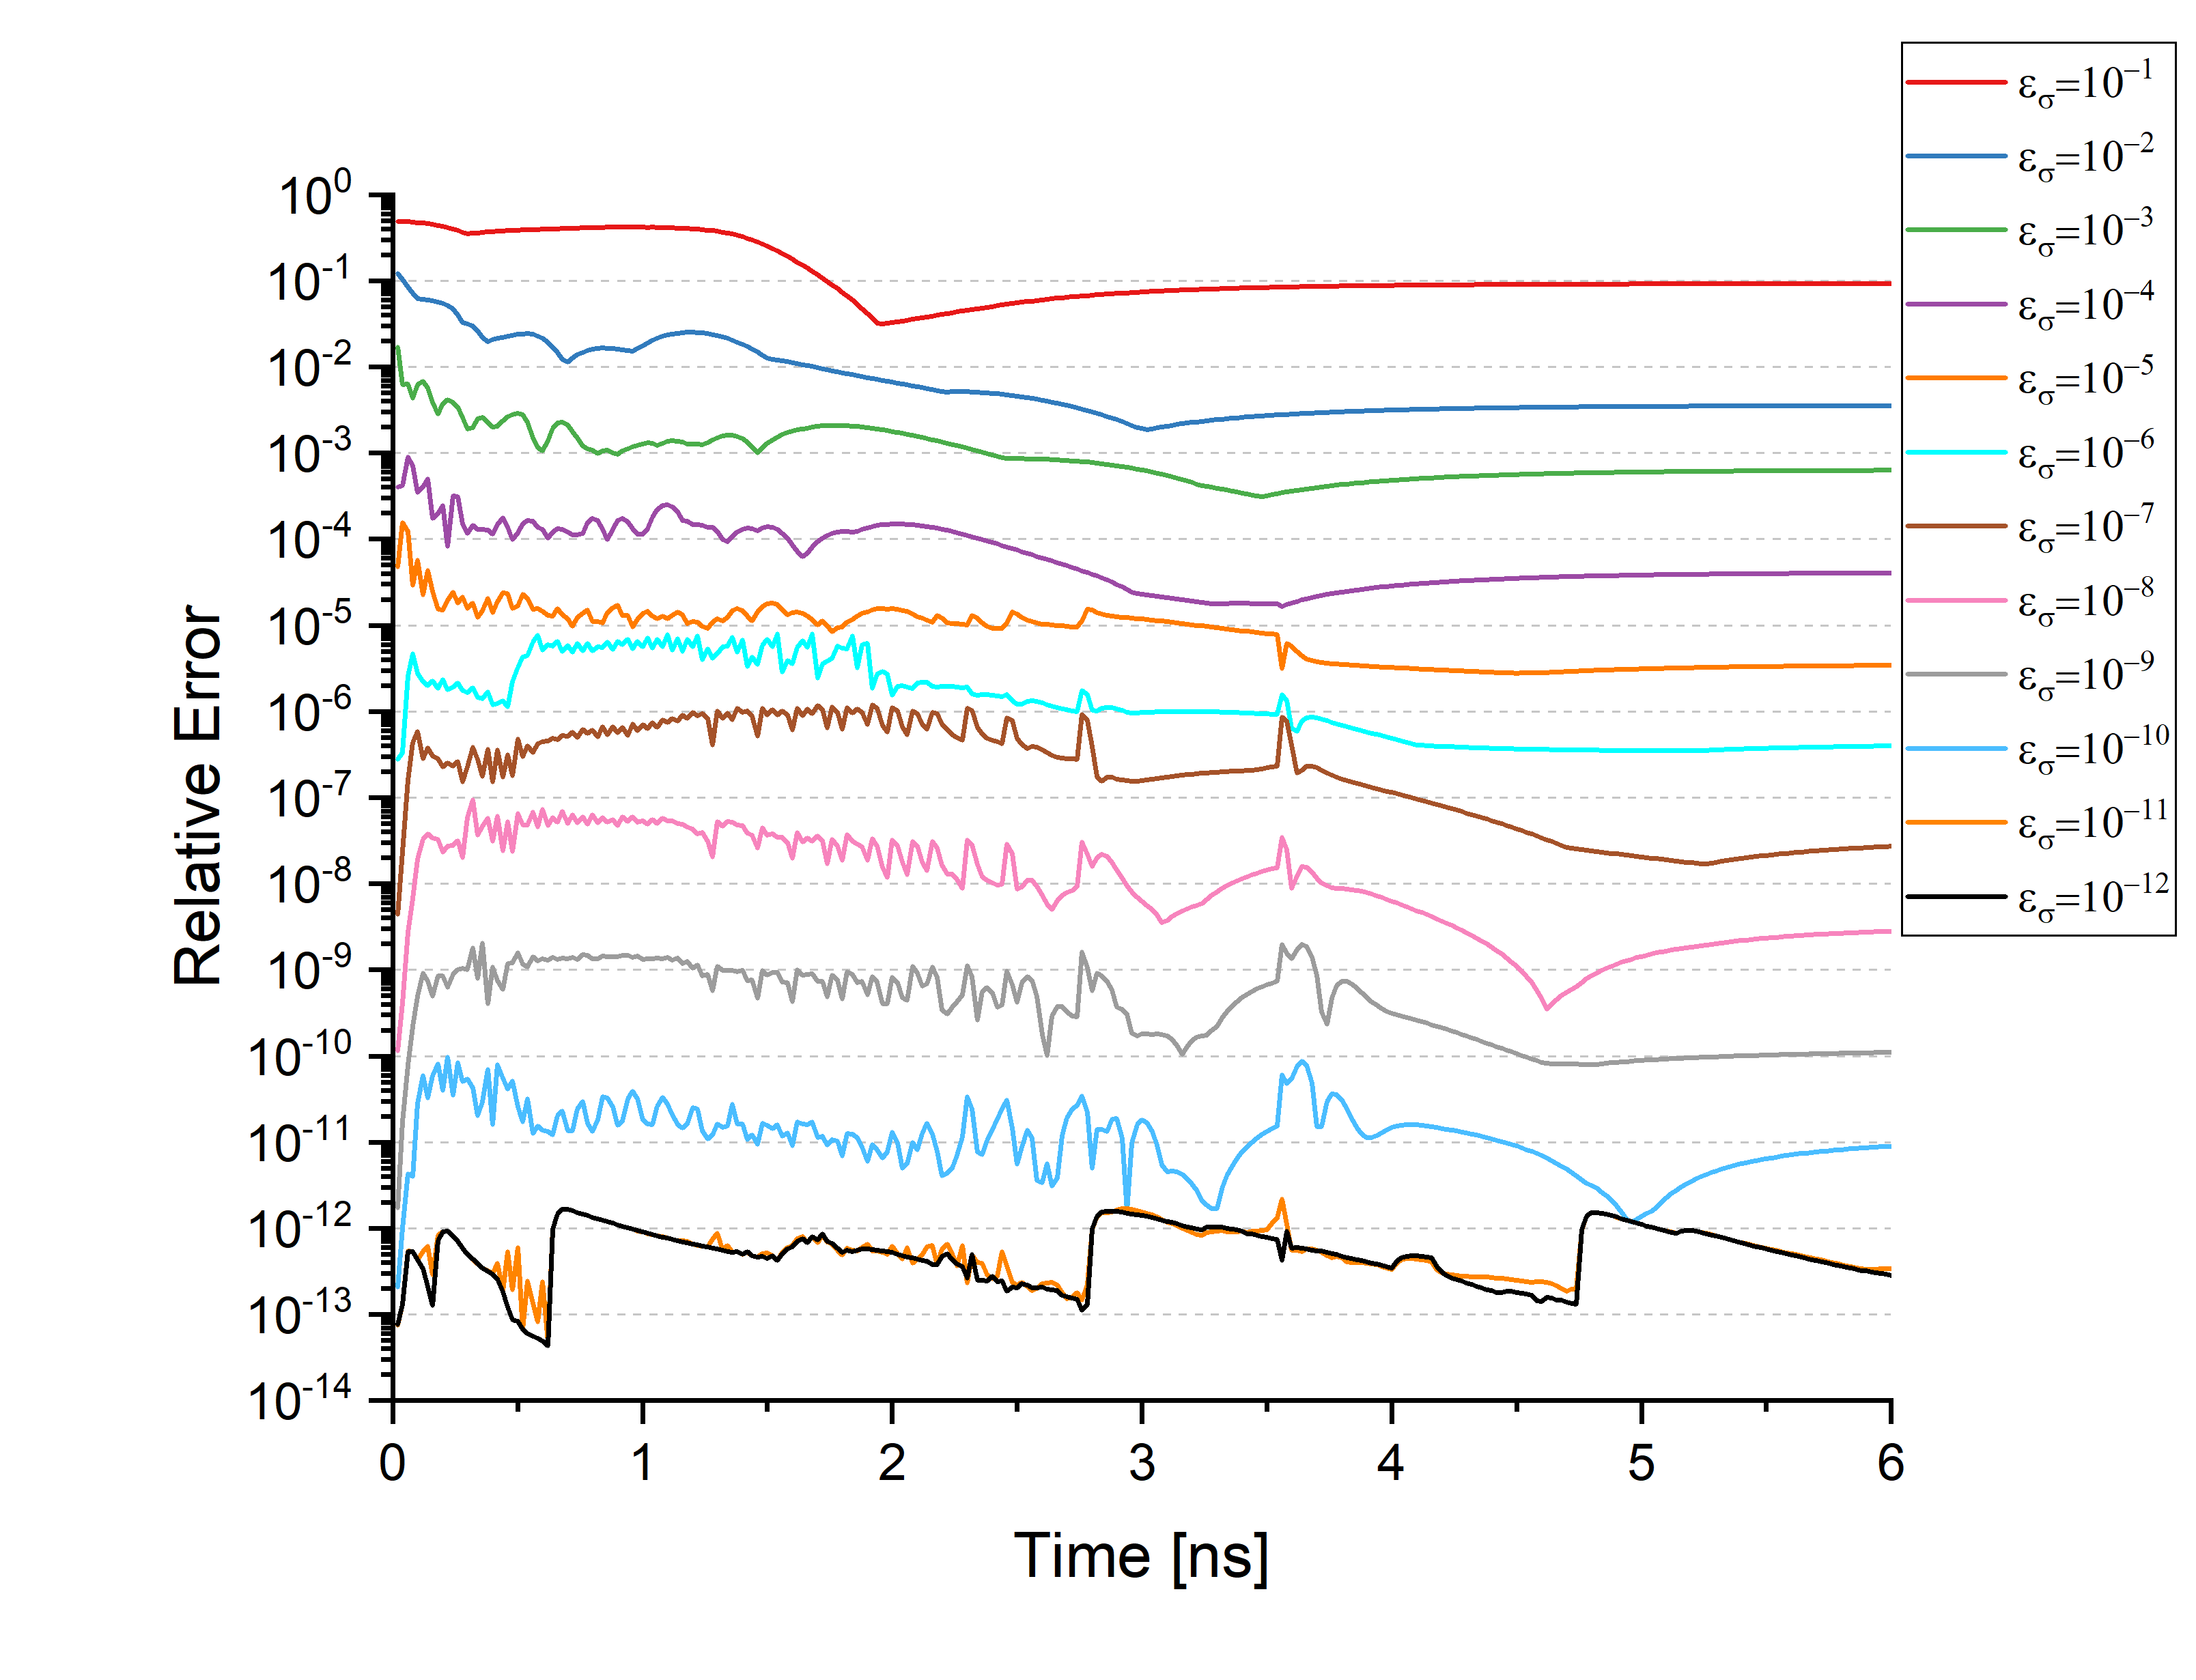
\includegraphics[width=0.5\textwidth]{refcase_E_rel_inf.png}}
		\caption{\label{fig:ref_errs_inf}
			Relative Error of the MLOQD-POD ROM solution to the F-C test problem versus the high order solution in $\infty$ norm for various $\varepsilon_\sigma$ values}
	\end{figure}

	\ind The MLOQD-POD ROM also has the capability to use an incomplete database of QD factors. For instance, using the database formed for the original F-C test described in Sec. \ref{sec:mpod_test} the MLOQD-POD ROM may solve the F-C test with a refined time step length. In this case the problem is solved over more instants of time than are included in the database. QD factors for the instants of time not included in the database are calculated with linear interpolation between the recorded values \cite{Bui-Thanh-2003}. Figure \ref{fig:errors_dt-0.01} shows the  relative error in $L_1$-norm of the MLOQD-POD ROM solution computed with $\Delta t \! = \! 1\! \times\! 10^{-2}$ ns using various values of $\varepsilon_{\sigma}$. Figure \ref{fig:errors_dt-0.005}  presents the relative error in $L_1$-norm of the solutions computed with $\Delta t \! = \! 5\! \times  \! 10^{-3}$ ns. Figure \ref{fig:errors_dt-0.002}  presents the relative error in $L_1$-norm of the solutions computed with $\Delta t \! = \! 2\! \times  \! 10^{-3}$ ns. The reference solution is recalculated for each time step length to find relative errors, and the database generated with $\Delta t = 2\times 10^{-2}$ ns is used for all MLOQD-POD ROMs. The relative error of these MLOQD-POD ROMs saturates at $\varepsilon_\sigma=10^{-4}$, thus the shown results are for only $\varepsilon_\sigma \geq 10^{-4}$. For all cases the error at the early time steps is large and drops several orders of magnitude as the problem progresses, which can be attributed to how the dynamics of the problem evolve. The radiation front changes most rapidly at the start of the problem during initial wave formation. The group QD factors experience similarly rapid changes as a result as depicted in Figs. \ref{fig:qdf_g2_recomps}, \ref{fig:qdf_g3_recomps} and \ref{fig:qdf_g8_recomps}. Such swift changes may be difficult to estimate with linear interpolation, limiting the accuracy of the ROM at early times. When comparing the relative error of each ROM the error at early instants of time does not significantly change, and at the final stage of the problem when the change rate of the solution is very small there is only an order of magnitude difference in the errors between the solutions computed with time steps $1\times10^{-2}$ ns and $2\times10^{-3}$ ns. The difference in time step length between these two cases is an order of 5, thus the error of the MLOQD-POD ROM is not very sensitive to how refined the time step length is compared to the reference case from which the approximate QD factors are generated.

	%=================================================================================
	% REDUCED TIME STEP ERRORS PLOT
	\begin{figure}[ht!]
		\centering
		\subfloat[Temperature relative error \label{subfig-1:MG_bc1000-t001_qdf1000-t002_Tavg_mlqd}]{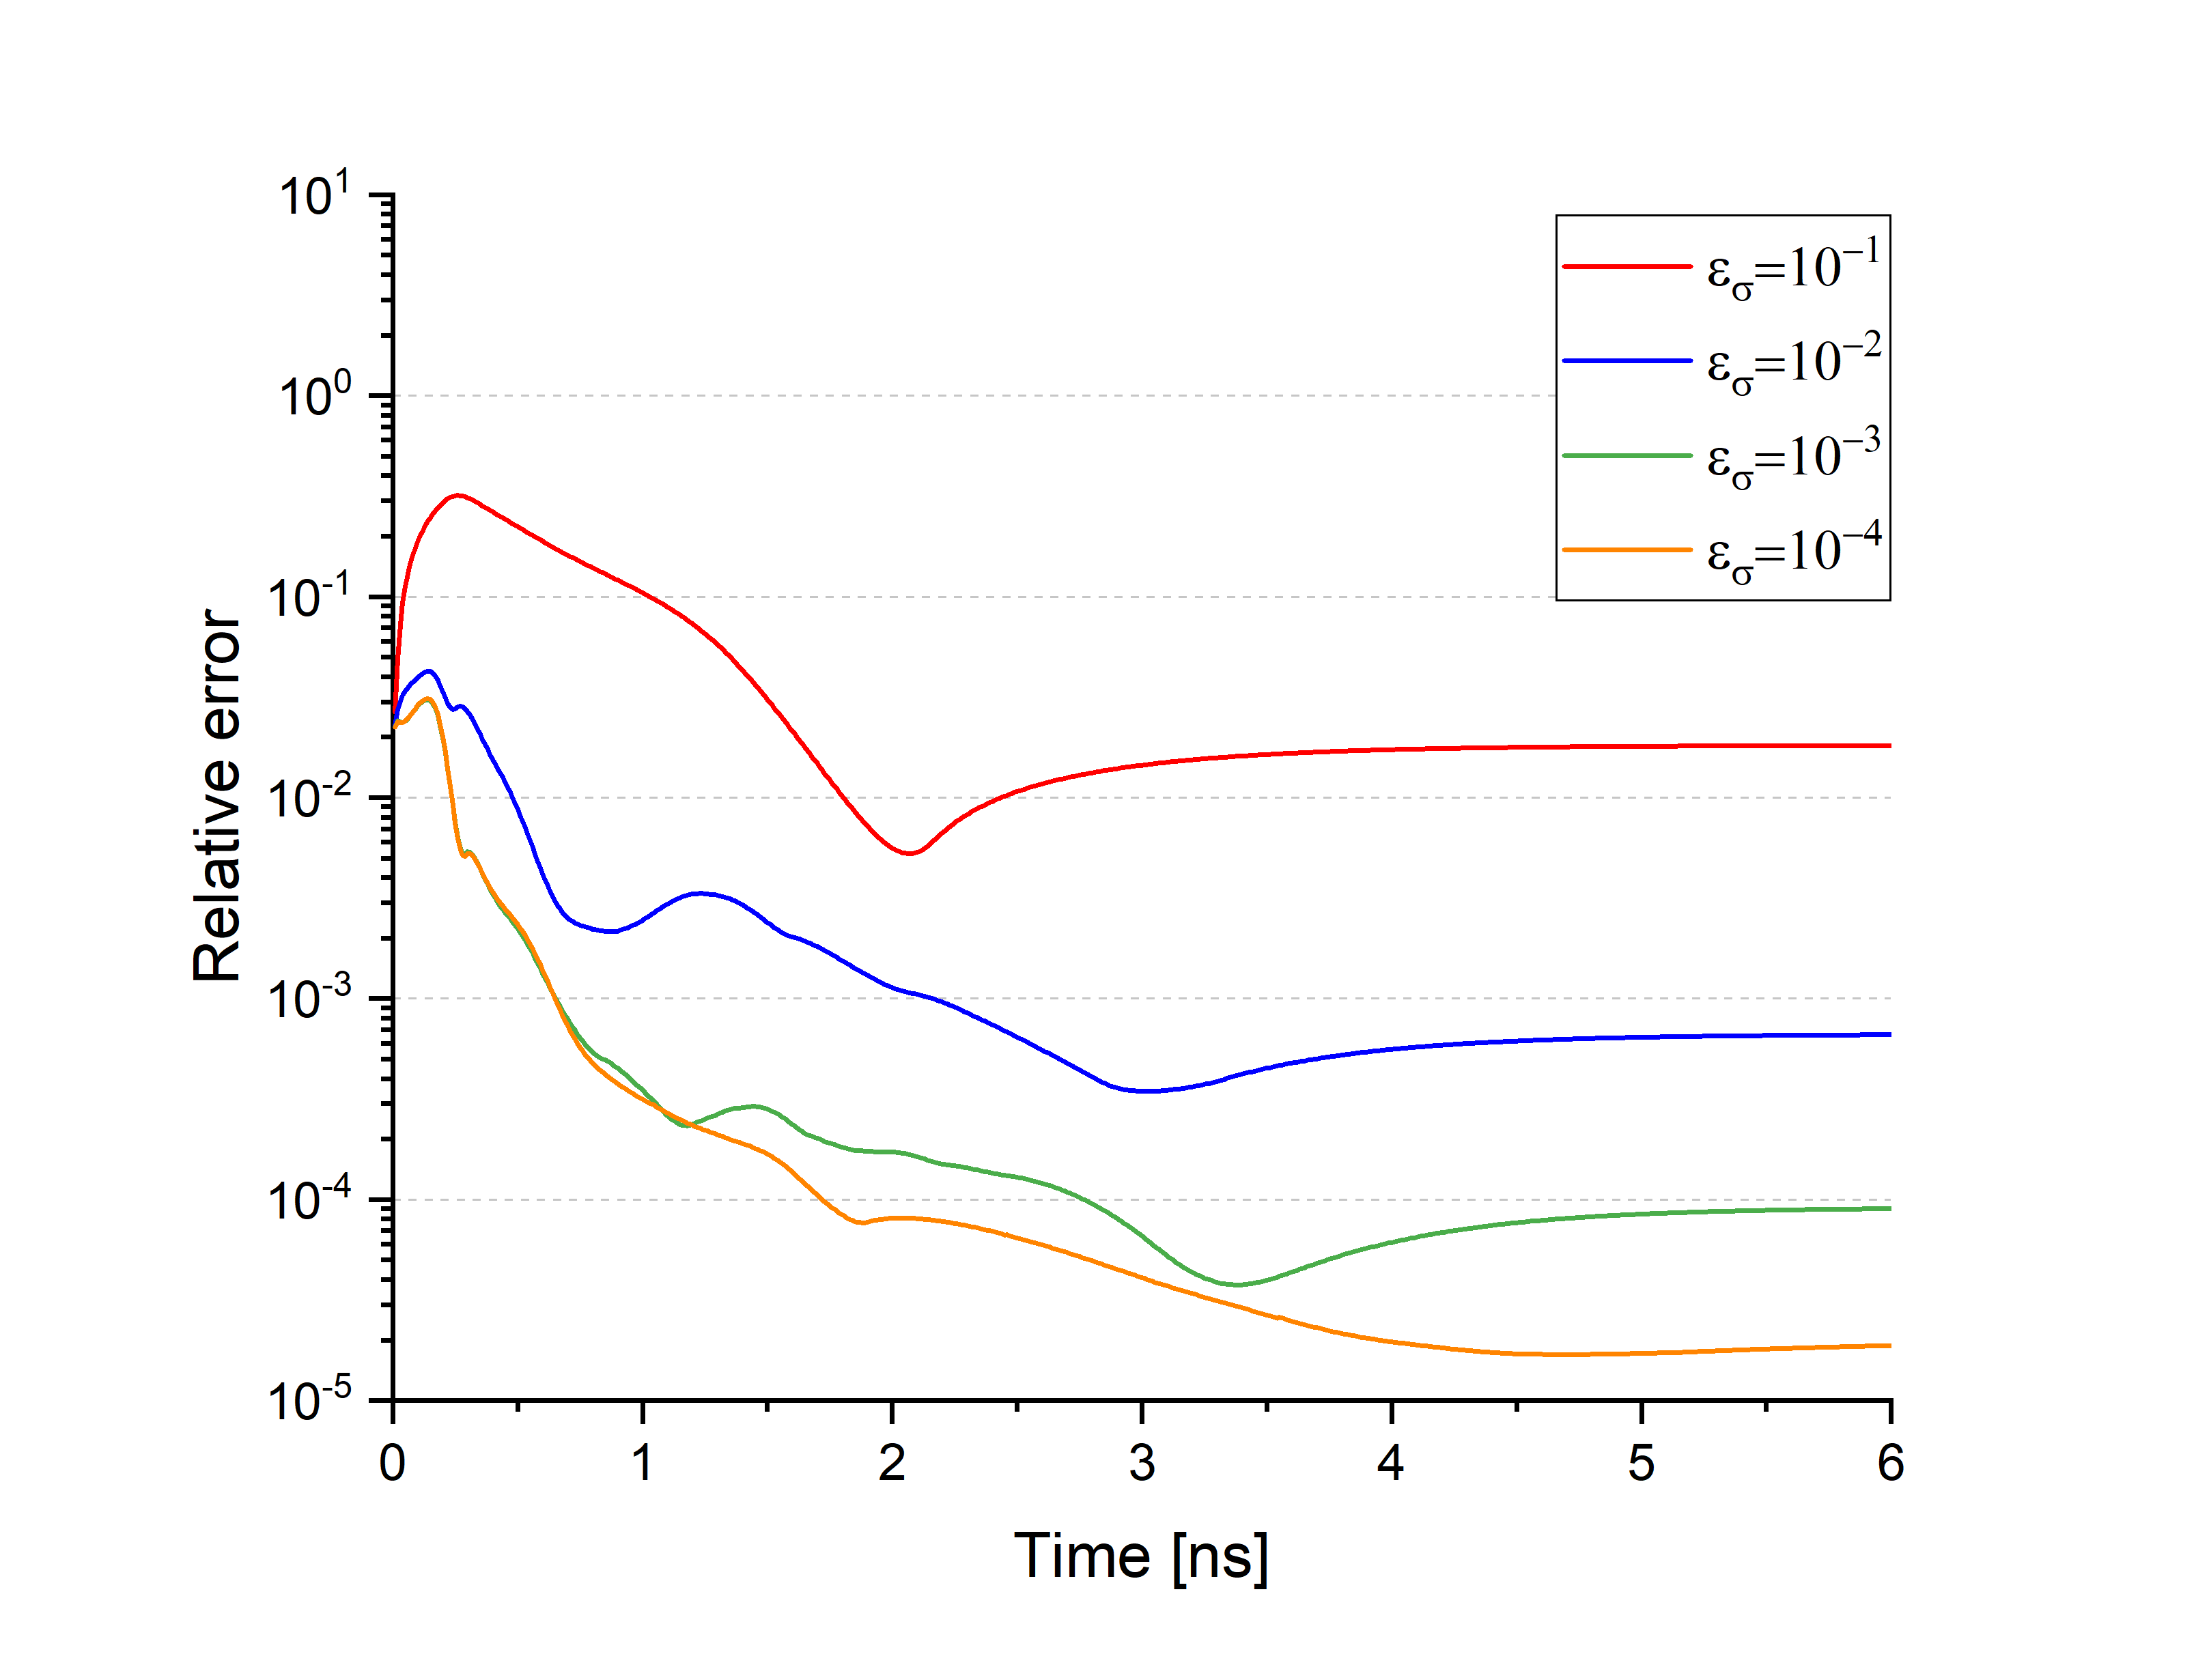
\includegraphics[width=0.5\textwidth]{MG_bc1000-t001_qdf1000-t002_Tavg_mlqd.png}}
		\subfloat[Energy density relative error \label{subfig-1:MG_bc1000-t001_qdf1000-t002_Eavg_mlqd}]{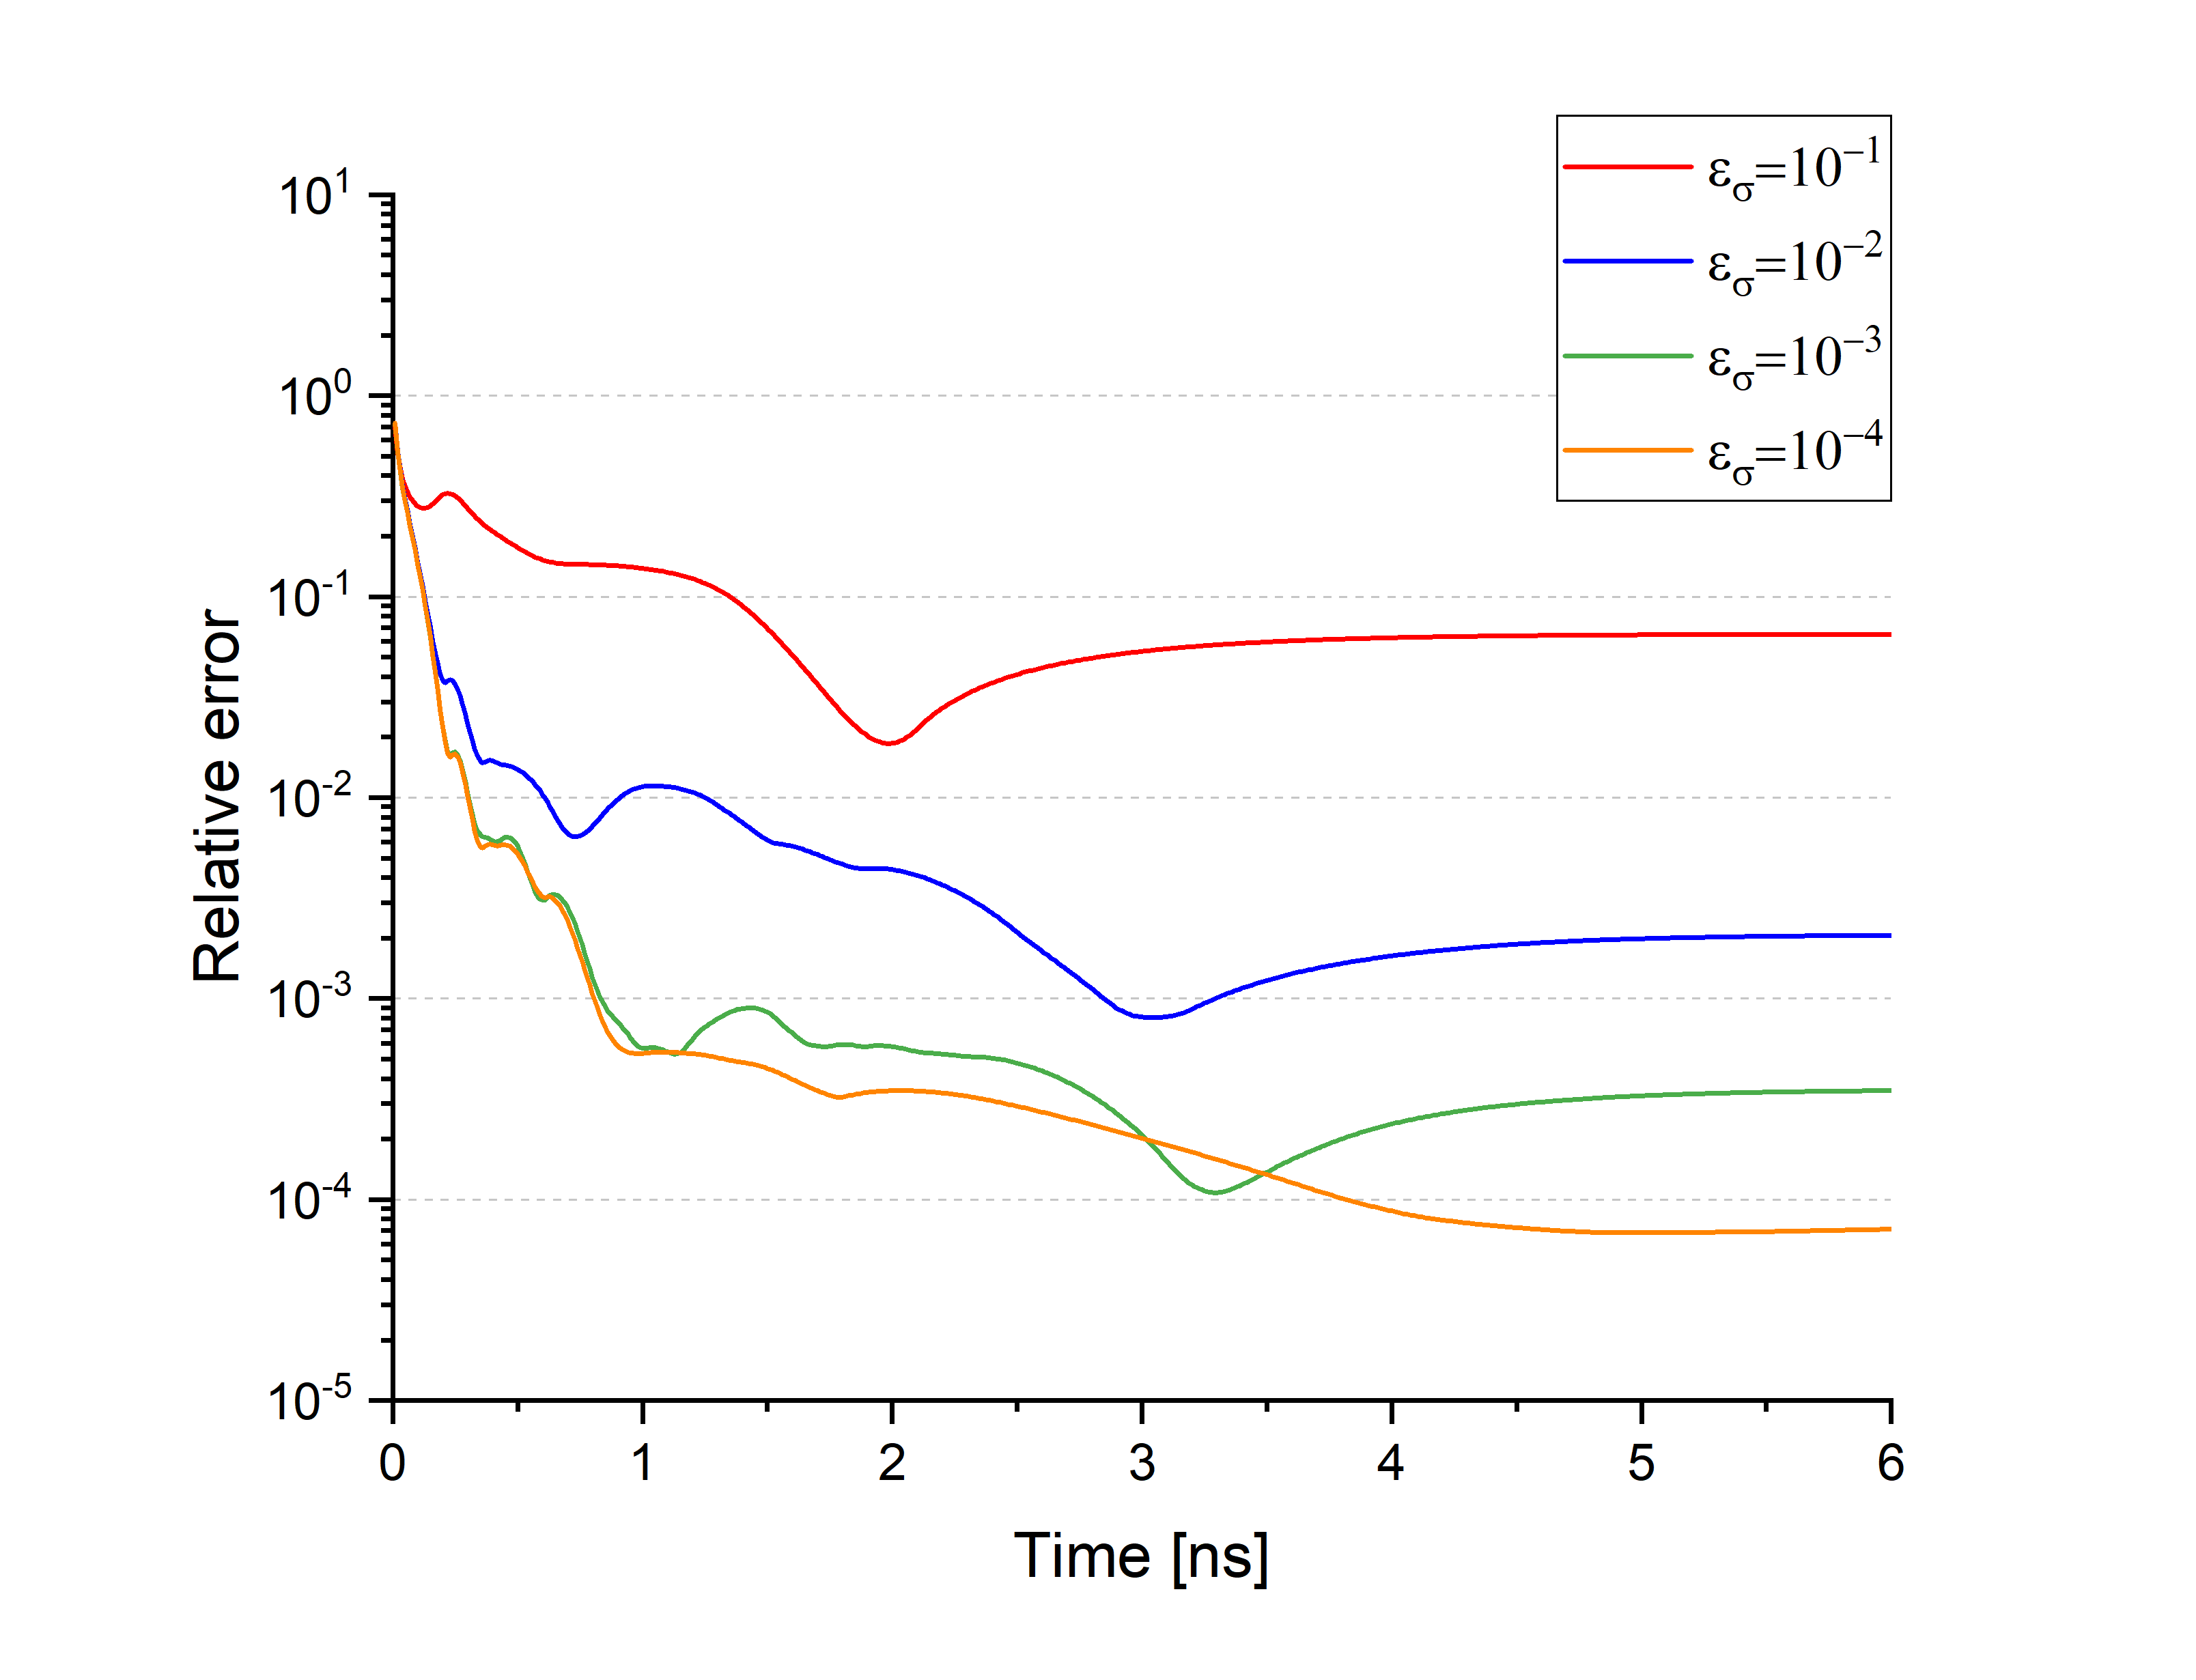
\includegraphics[width=0.5\textwidth]{MG_bc1000-t001_qdf1000-t002_Eavg_mlqd.png}}
		\caption{\label{fig:errors_dt-0.01}
			Relative error in the $L_1$-norm of MLOQD-POD ROM solutions  computed with $\Delta t\! =\! 1 \! \times \! 10^{-2}$~ns
			versus the reference TRT solution. The data for the MLOQD-POD ROM is generated with $\Delta t\! =\! 2 \! \times\!  10^{-2}$ ns. }
	\end{figure}

	\begin{figure}[ht!]
		\centering
		\subfloat[Temperature relative error \label{subfig-1:MG_bc1000-t0005_qdf1000-t002_Tavg_mlqd}]{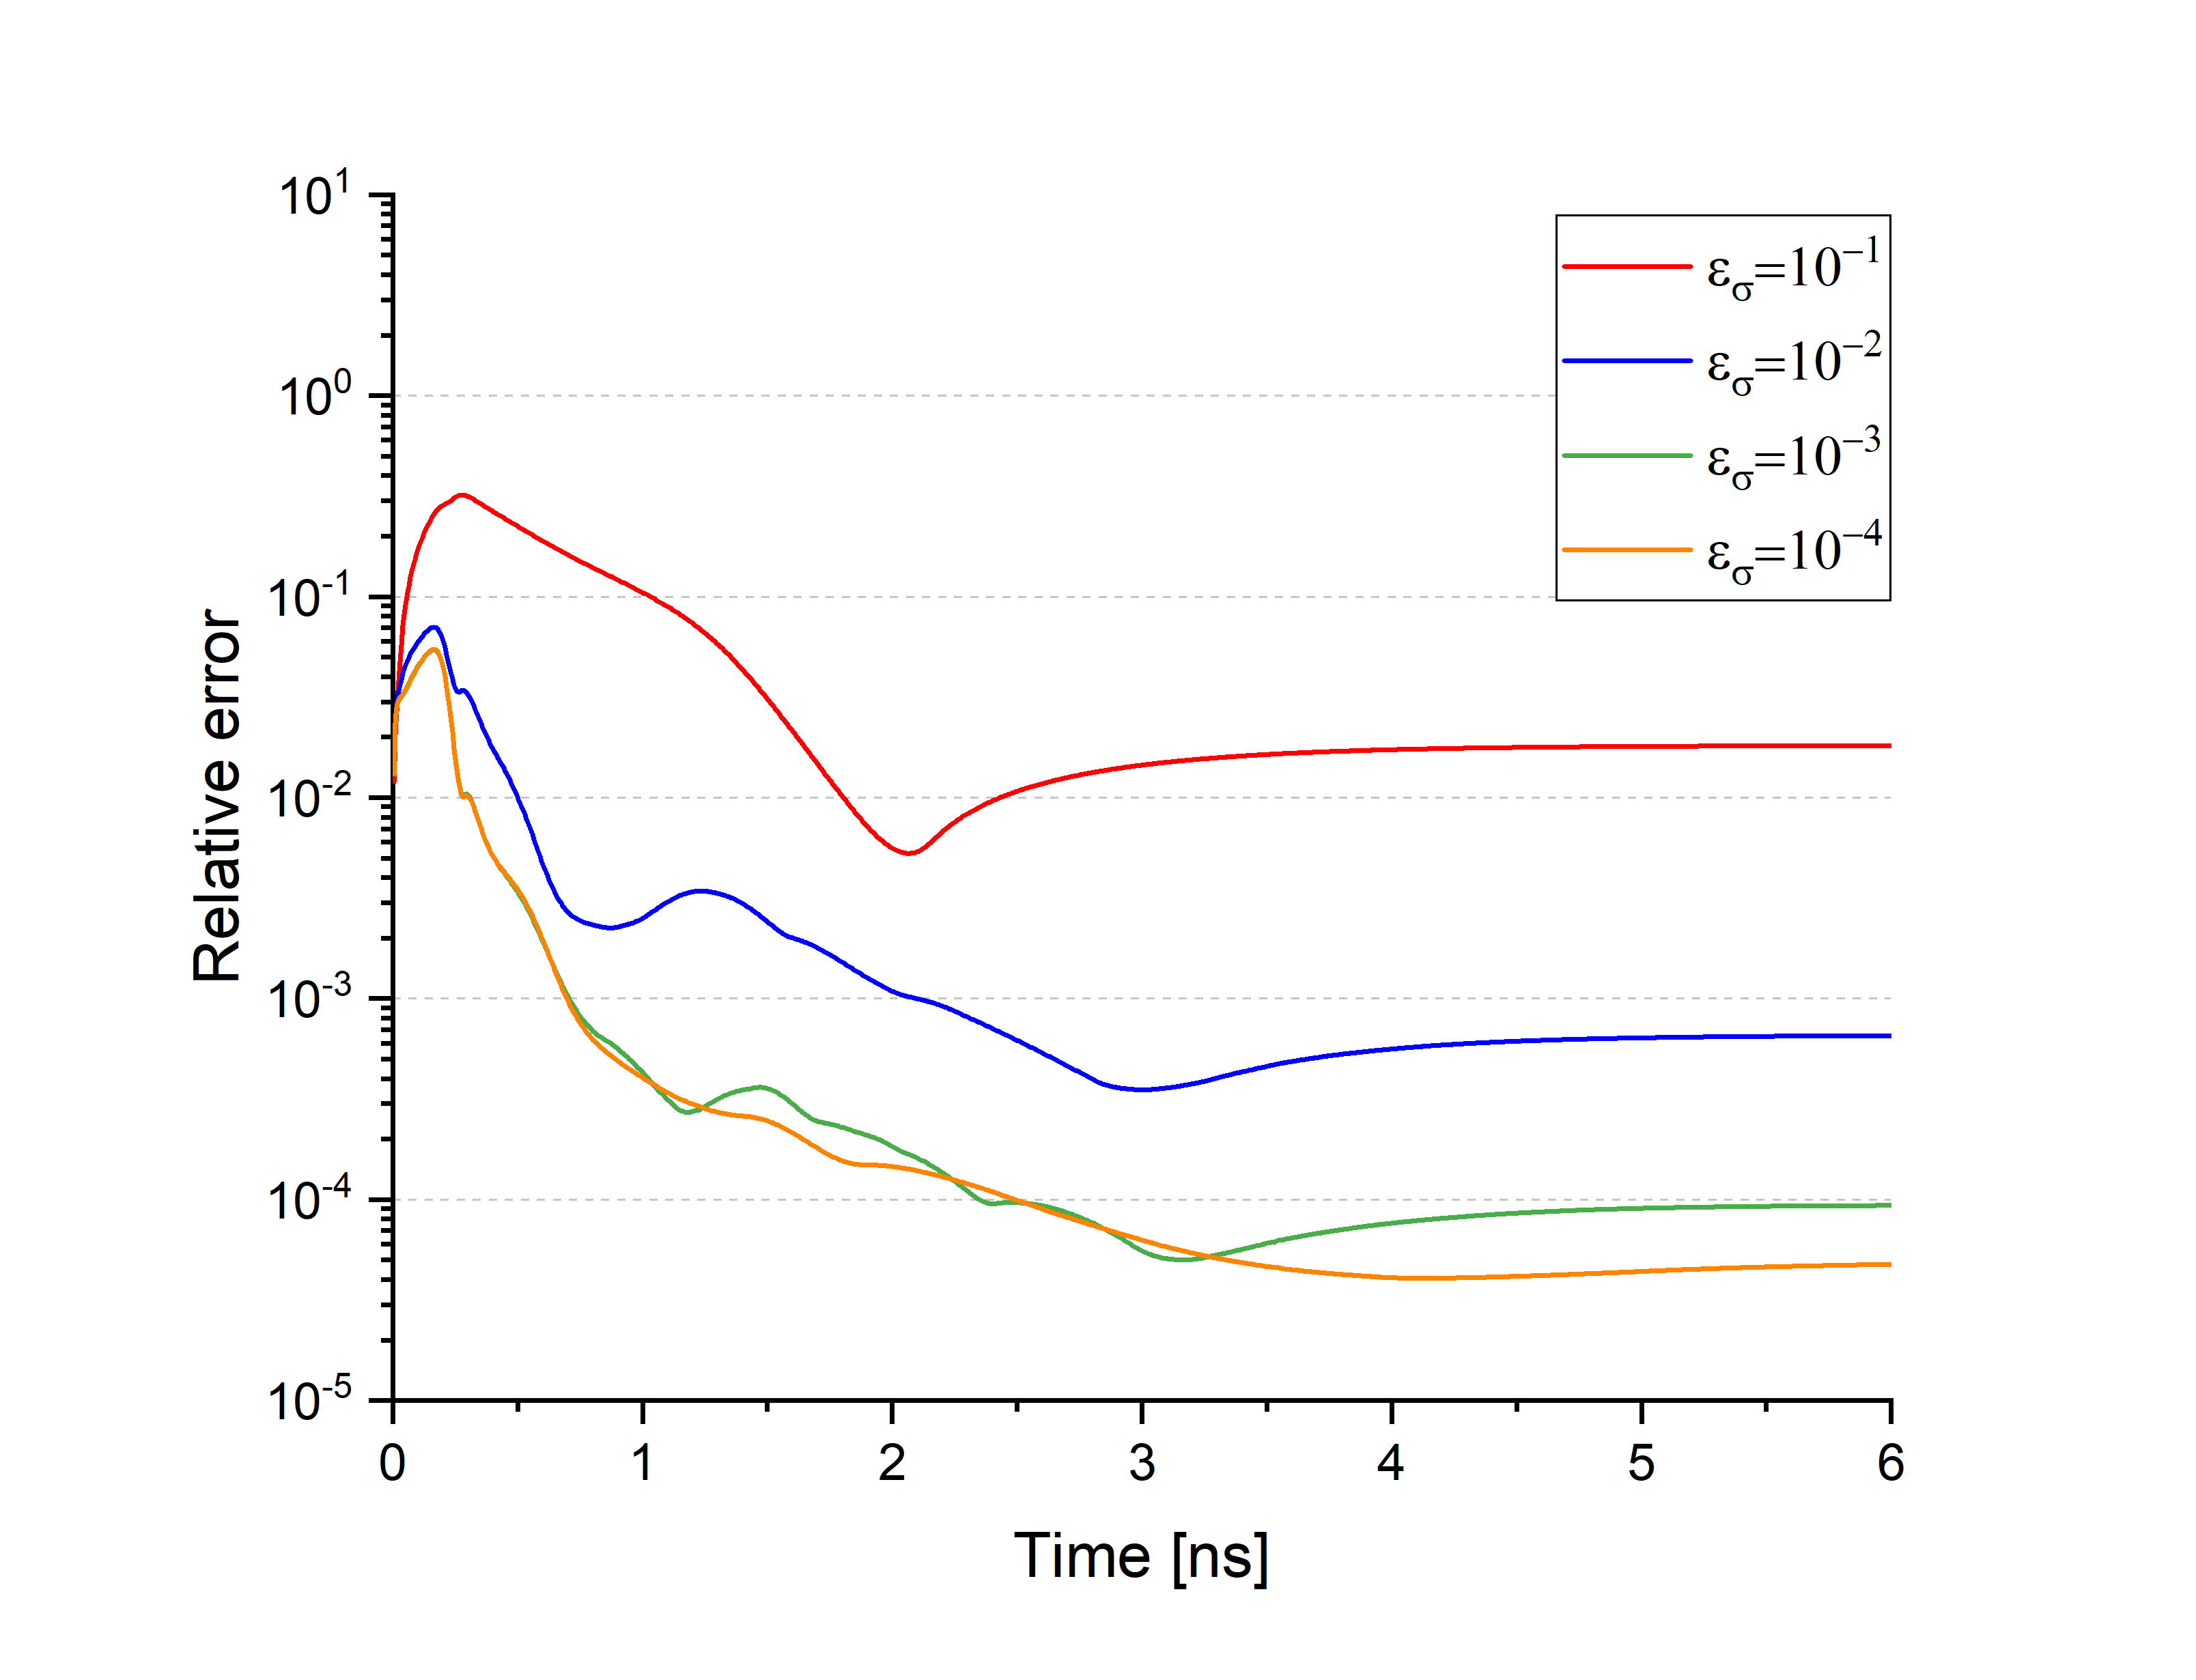
\includegraphics[width=0.5\textwidth]{MG_bc1000-t0005_qdf1000-t002_Tavg_mlqd.png}}
		\subfloat[Energy density relative error \label{subfig-1:MG_bc1000-t0005_qdf1000-t002_Eavg_mlqd}]{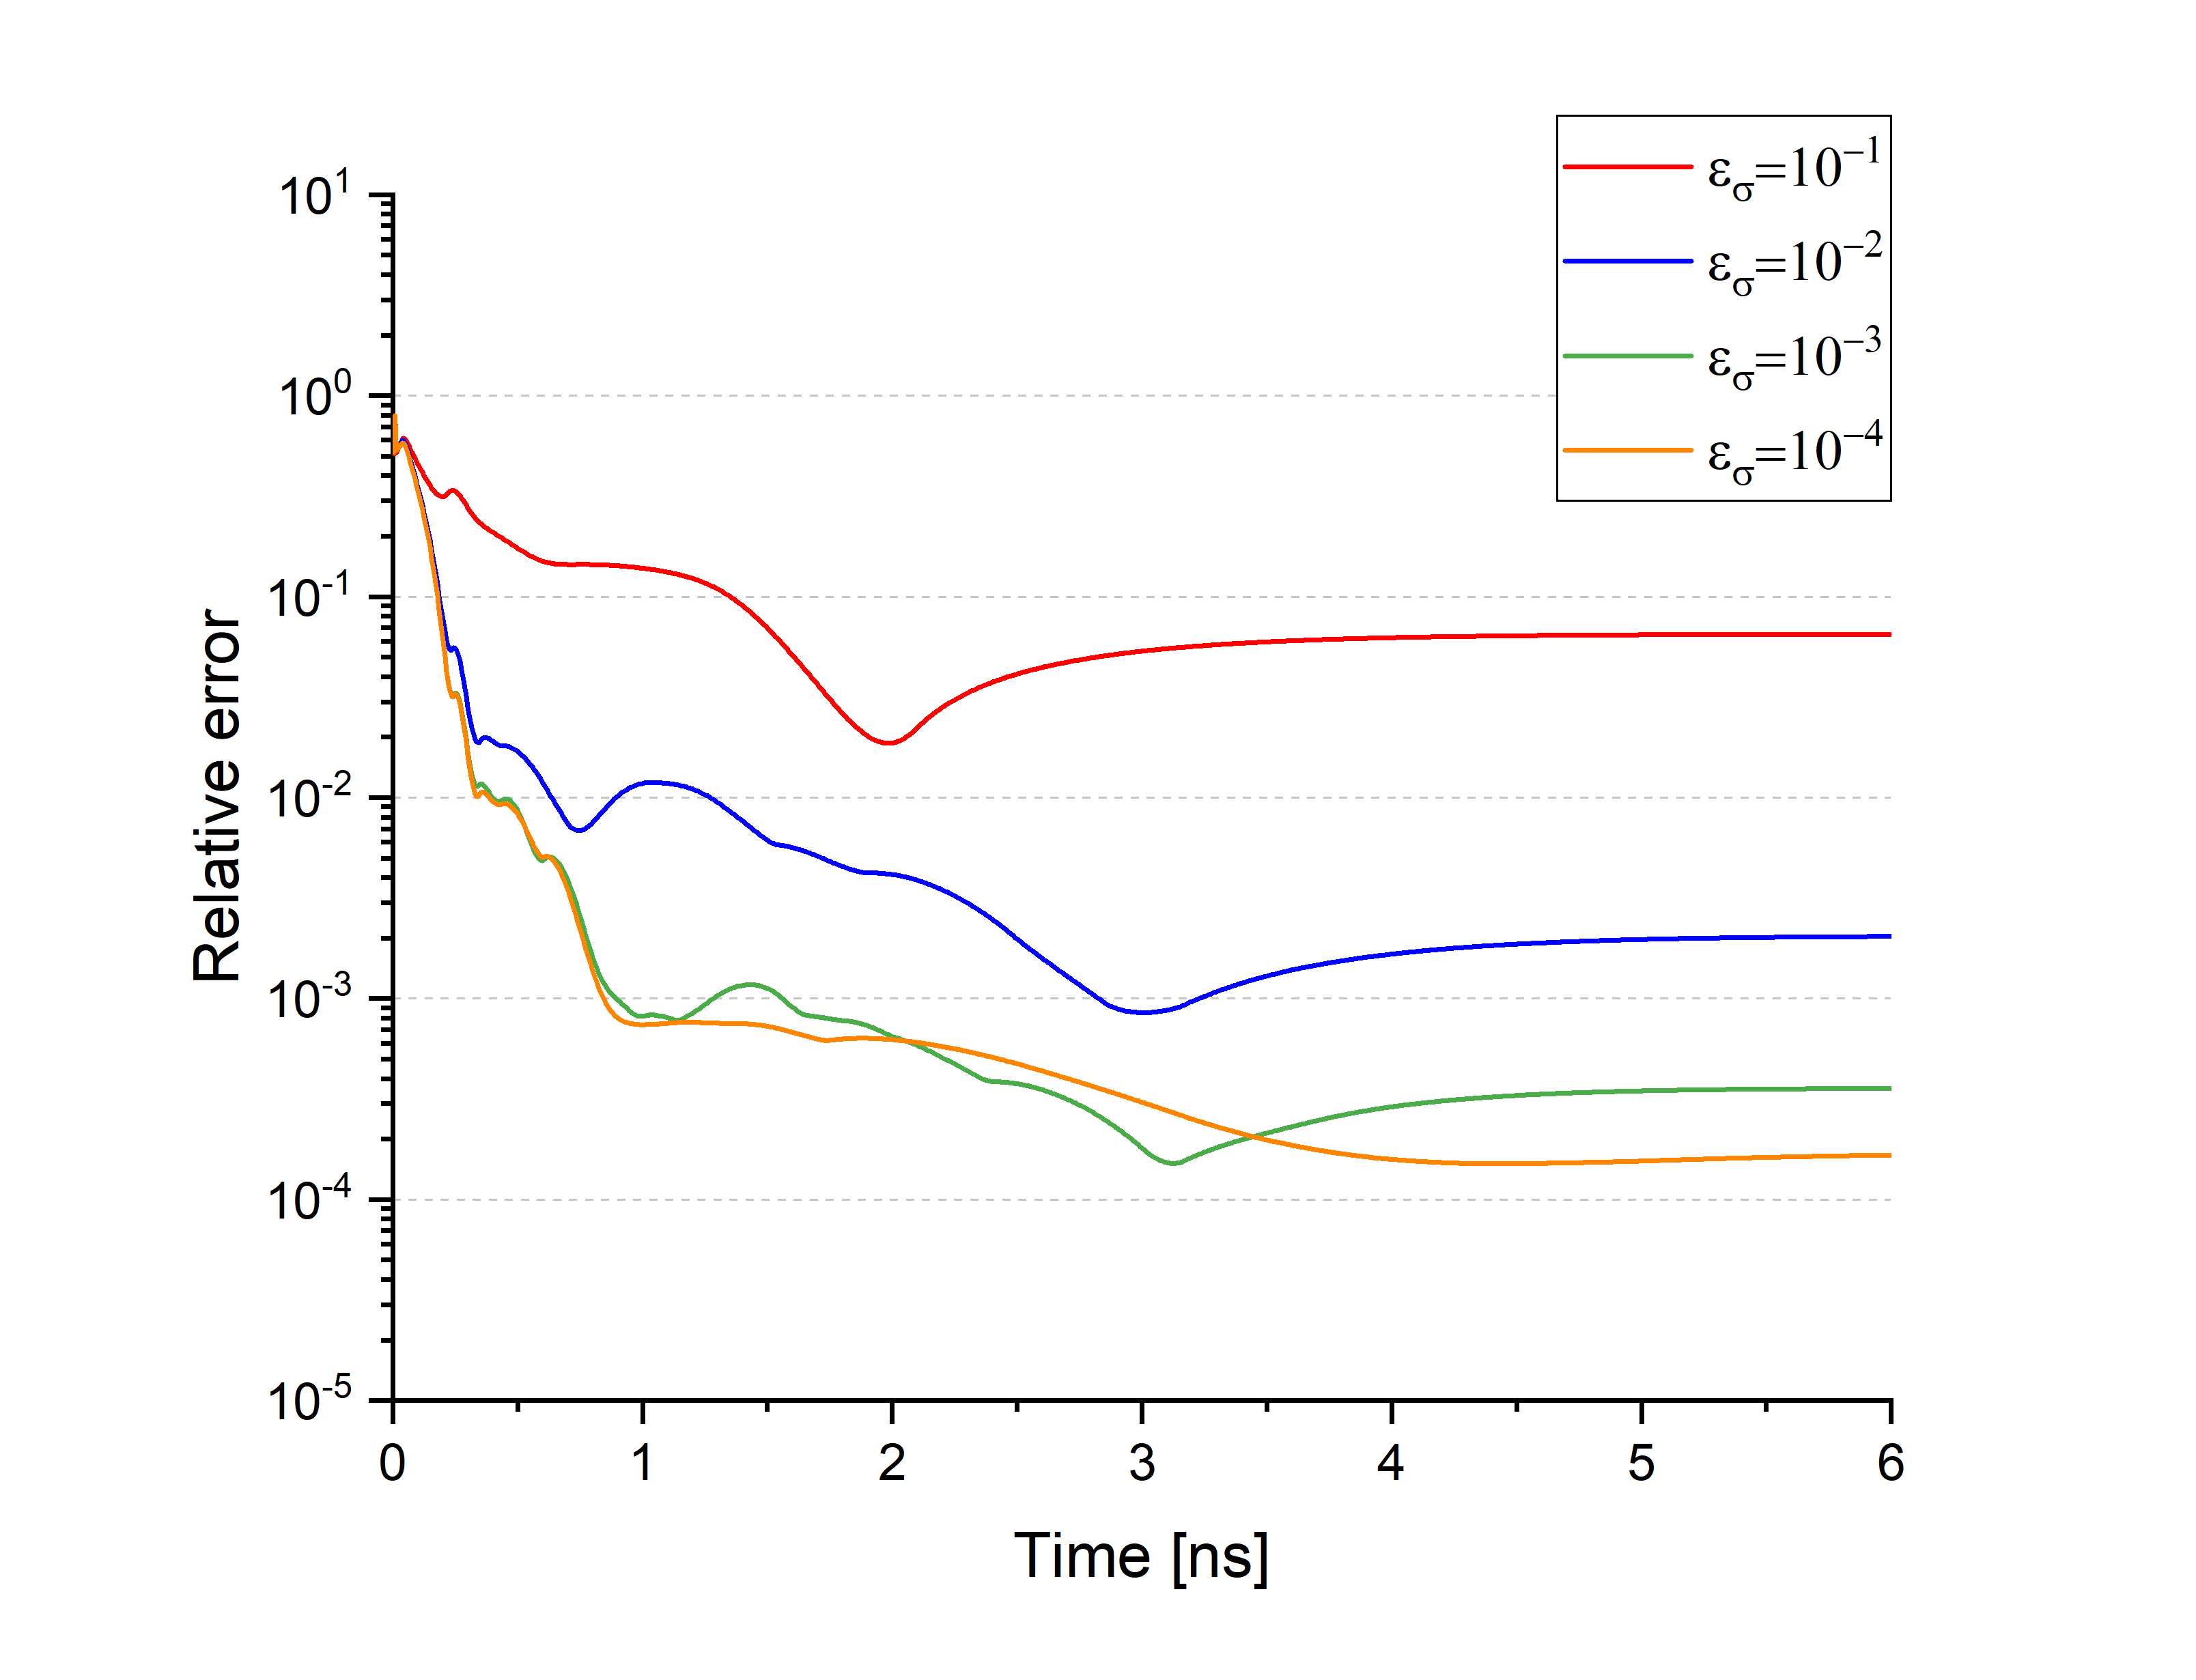
\includegraphics[width=0.5\textwidth]{MG_bc1000-t0005_qdf1000-t002_Eavg_mlqd.png}}
		\caption{\label{fig:errors_dt-0.005}
			Relative error in the $L_1$-norm of MLOQD-POD ROM solutions  computed with $\Delta t\! =\! 5 \! \times \! 10^{-3}$~ns
			versus the reference TRT solution. The data for the MLOQD-POD ROM is generated with $\Delta t\! =\! 2 \! \times\!  10^{-2}$ ns. }
	\end{figure}

	\begin{figure}[ht!]
		\centering
		\subfloat[Temperature relative error \label{subfig-1:MG_bc1000-t0002_qdf1000-t002_Tavg_mlqd}]{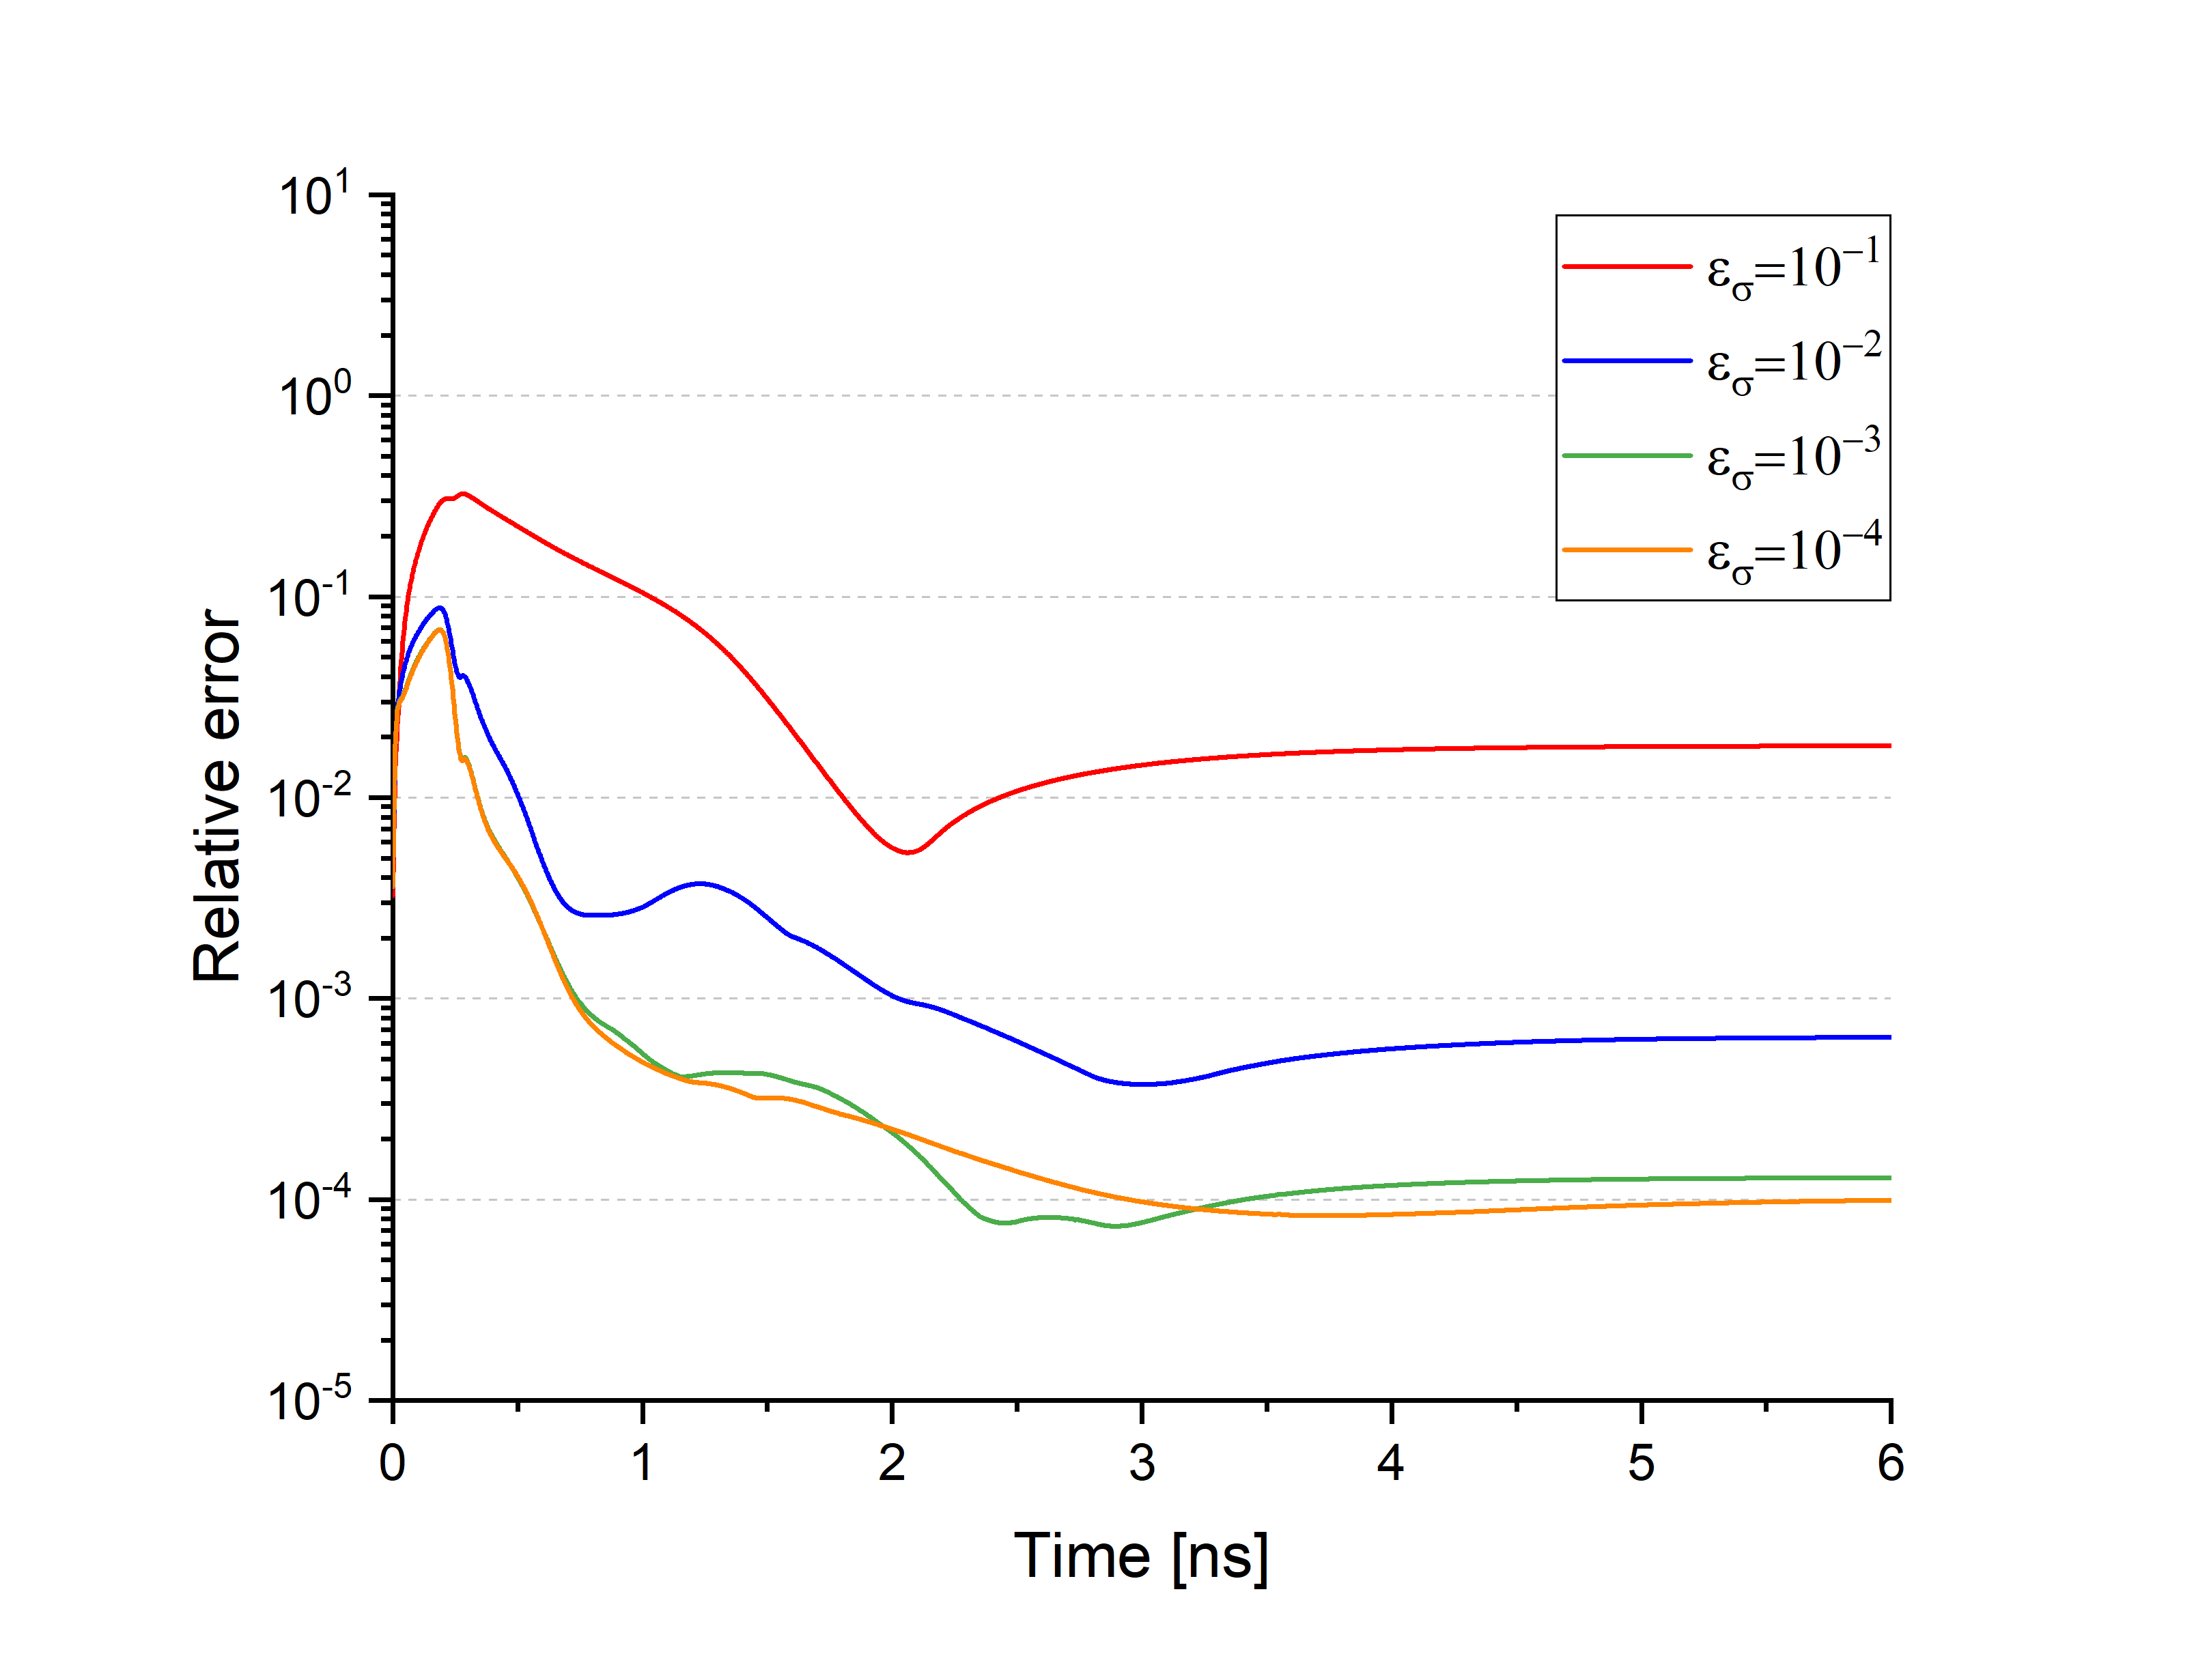
\includegraphics[width=0.5\textwidth]{MG_bc1000-t0002_qdf1000-t002_Tavg_mlqd.png}}
		\subfloat[Energy density relative error \label{subfig-1:MG_bc1000-t0002_qdf1000-t002_Eavg_mlqd}]{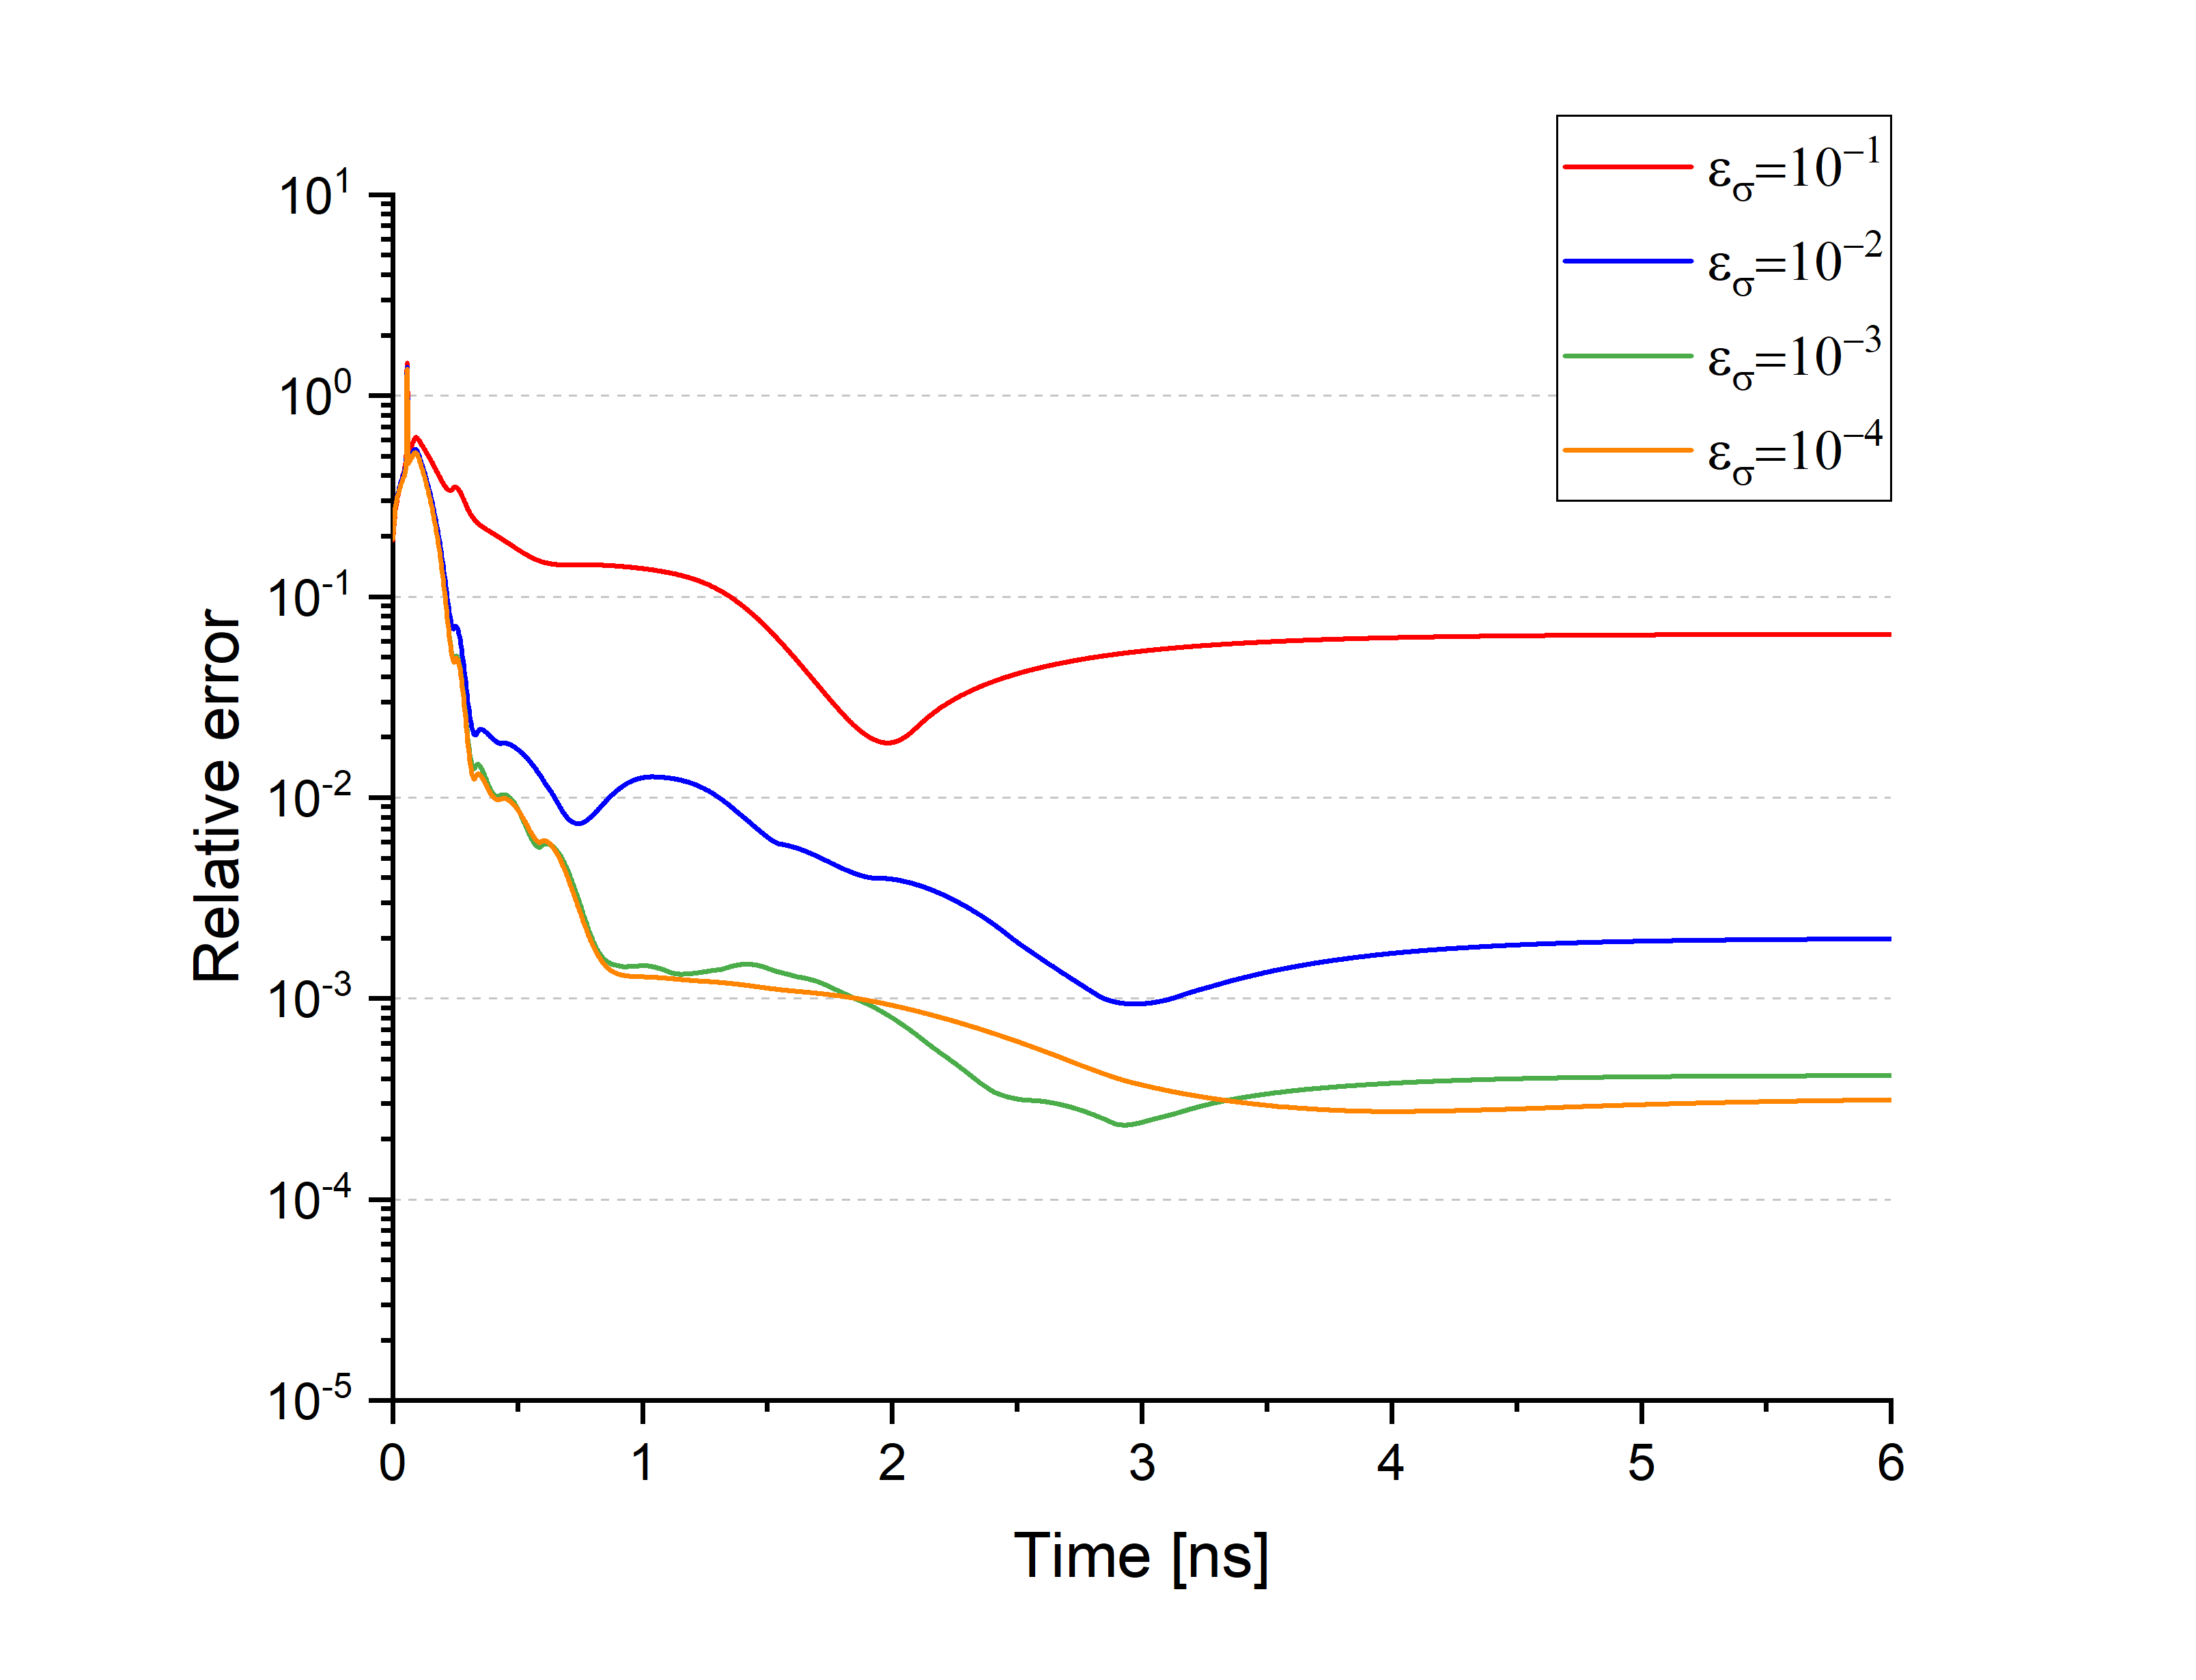
\includegraphics[width=0.5\textwidth]{MG_bc1000-t0002_qdf1000-t002_Eavg_mlqd.png}}
		\caption{\label{fig:errors_dt-0.002}
			Relative error in the $L_1$-norm of MLOQD-POD ROM solutions  computed with $\Delta t\! =\! 2 \! \times \! 10^{-3}$~ns
			versus the reference TRT solution. The data for the MLOQD-POD ROM is generated with $\Delta t\! =\! 2 \! \times\!  10^{-2}$ ns. }
	\end{figure}

	\ind The MLOQD-POD ROM can be further extended to develop a parameterized ROM for a class of TRT problems using QD factors estimated from a set of base cases. In this study we consider a ROM parameterized with respect to the temperature $T_{in}$ of incoming radiation at the left boundary. A database of the group QD factors for problems with two selected temperatures of incoming radiation  $T_{in}^{(1)}$ and $T_{in}^{(2)}$ is constructed. The MLOQD-POD ROM solutions of TRT problems with incoming radiation at some given temperature are calculated using group QD factors obtained by linear interpolation between values in the database. Results are presented for three parameterized ROMs. One model uses $T_{in}^{(1)}~=~1$~KeV and $T_{in}^{(2)}=0.98$ KeV. The second model is formed with  $T_{in}^{(1)}=1$ KeV and $T_{in}^{(2)}=0.96$ KeV. The third is formed with  $T_{in}^{(1)}=1$ KeV and $T_{in}^{(2)}=0.92$ KeV. The databases are generated for $\Delta t = 2\times10^{-2}$ ns. Figure \ref{fig:errors_bc_T=990} shows  the  relative error in $L_1$-norm in the solution  for $T_{in}=0.99$ KeV computed by means of first parameterized MLOQD-POD ROM with various values of $\varepsilon_{\sigma}$. Figure \ref{fig:errors_bc_T=980} presents the relative error of the MLOQD-POD ROM solution  for $T_{in}= 0.98$ KeV obtained from the second model that is parameterized with a larger interval of  $[T_{in}^{(1)},T_{in}^{(2)}]$. Figure \ref{fig:errors_bc_T=960} presents the relative error of the MLOQD-POD ROM solution  for $T_{in}= 0.96$ KeV obtained from the third model that is parameterized with the largest interval of  $[T_{in}^{(1)},T_{in}^{(2)}]$. The reference solution is computed for each value of $T_{in}$ to obtain relative errors. The error in the MLOQD-POD ROM saturates at $\varepsilon_\sigma=10^{-6}$ and smaller values are not shown. Compared to the ROMs that used a reduced time step length compared to the database, the error displayed here is more uniform across time, and the lowest error found is smaller. As the interval $[T_{in}^{(1)},T_{in}^{(2)}]$ increases the error at $\varepsilon_\sigma=10^{-6}$ increases. However, the error associated with $\varepsilon_\sigma=10^{-1}$ does not visibly change on the plots shown.
	
	%=================================================================================
	% BOUNDARY CONDITION DATABASE ERRORS PLOT
	\begin{figure}[ht!]
		\centering
		\subfloat[Temperature relative error \label{subfig:MG_bc990-t002_qdf1000-980-t002_Tavg_mlqd}]{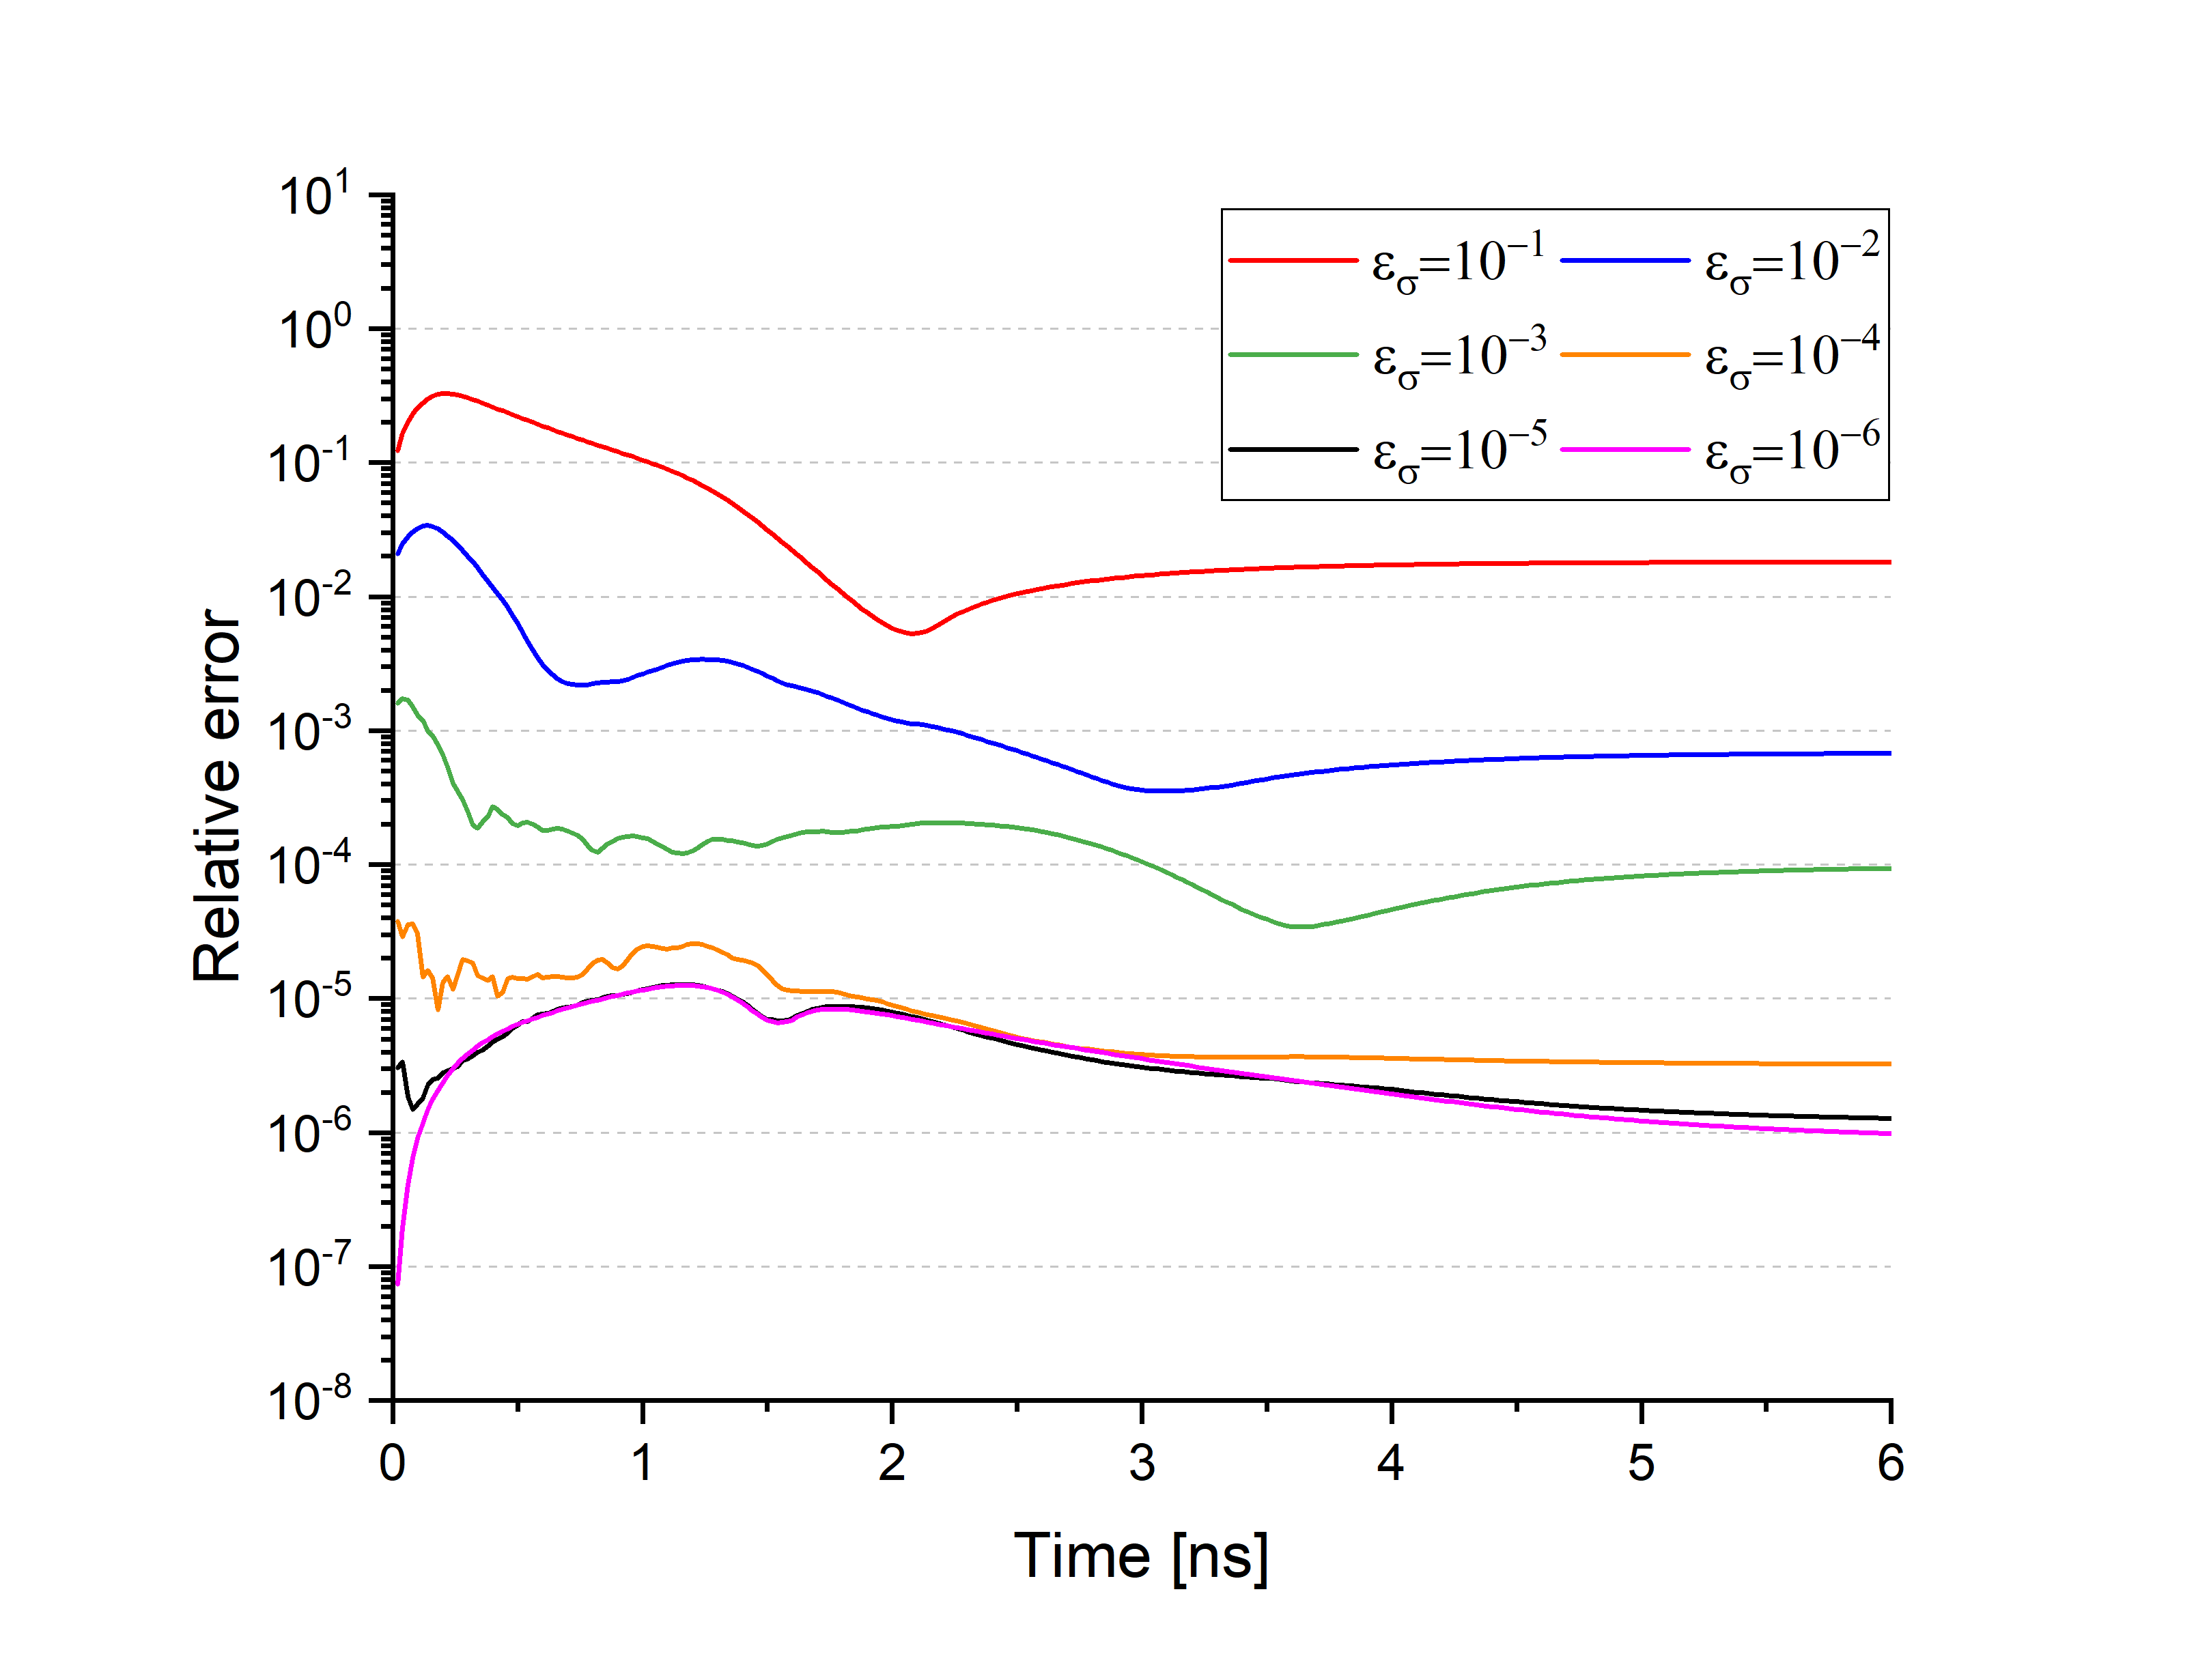
\includegraphics[width=0.5\textwidth]{MG_bc990-t002_qdf1000-980-t002_Tavg_mlqd.png}}
		\subfloat[Energy density relative error \label{subfig:MG_bc990-t002_qdf1000-980-t002_Eavg_mlqd}]{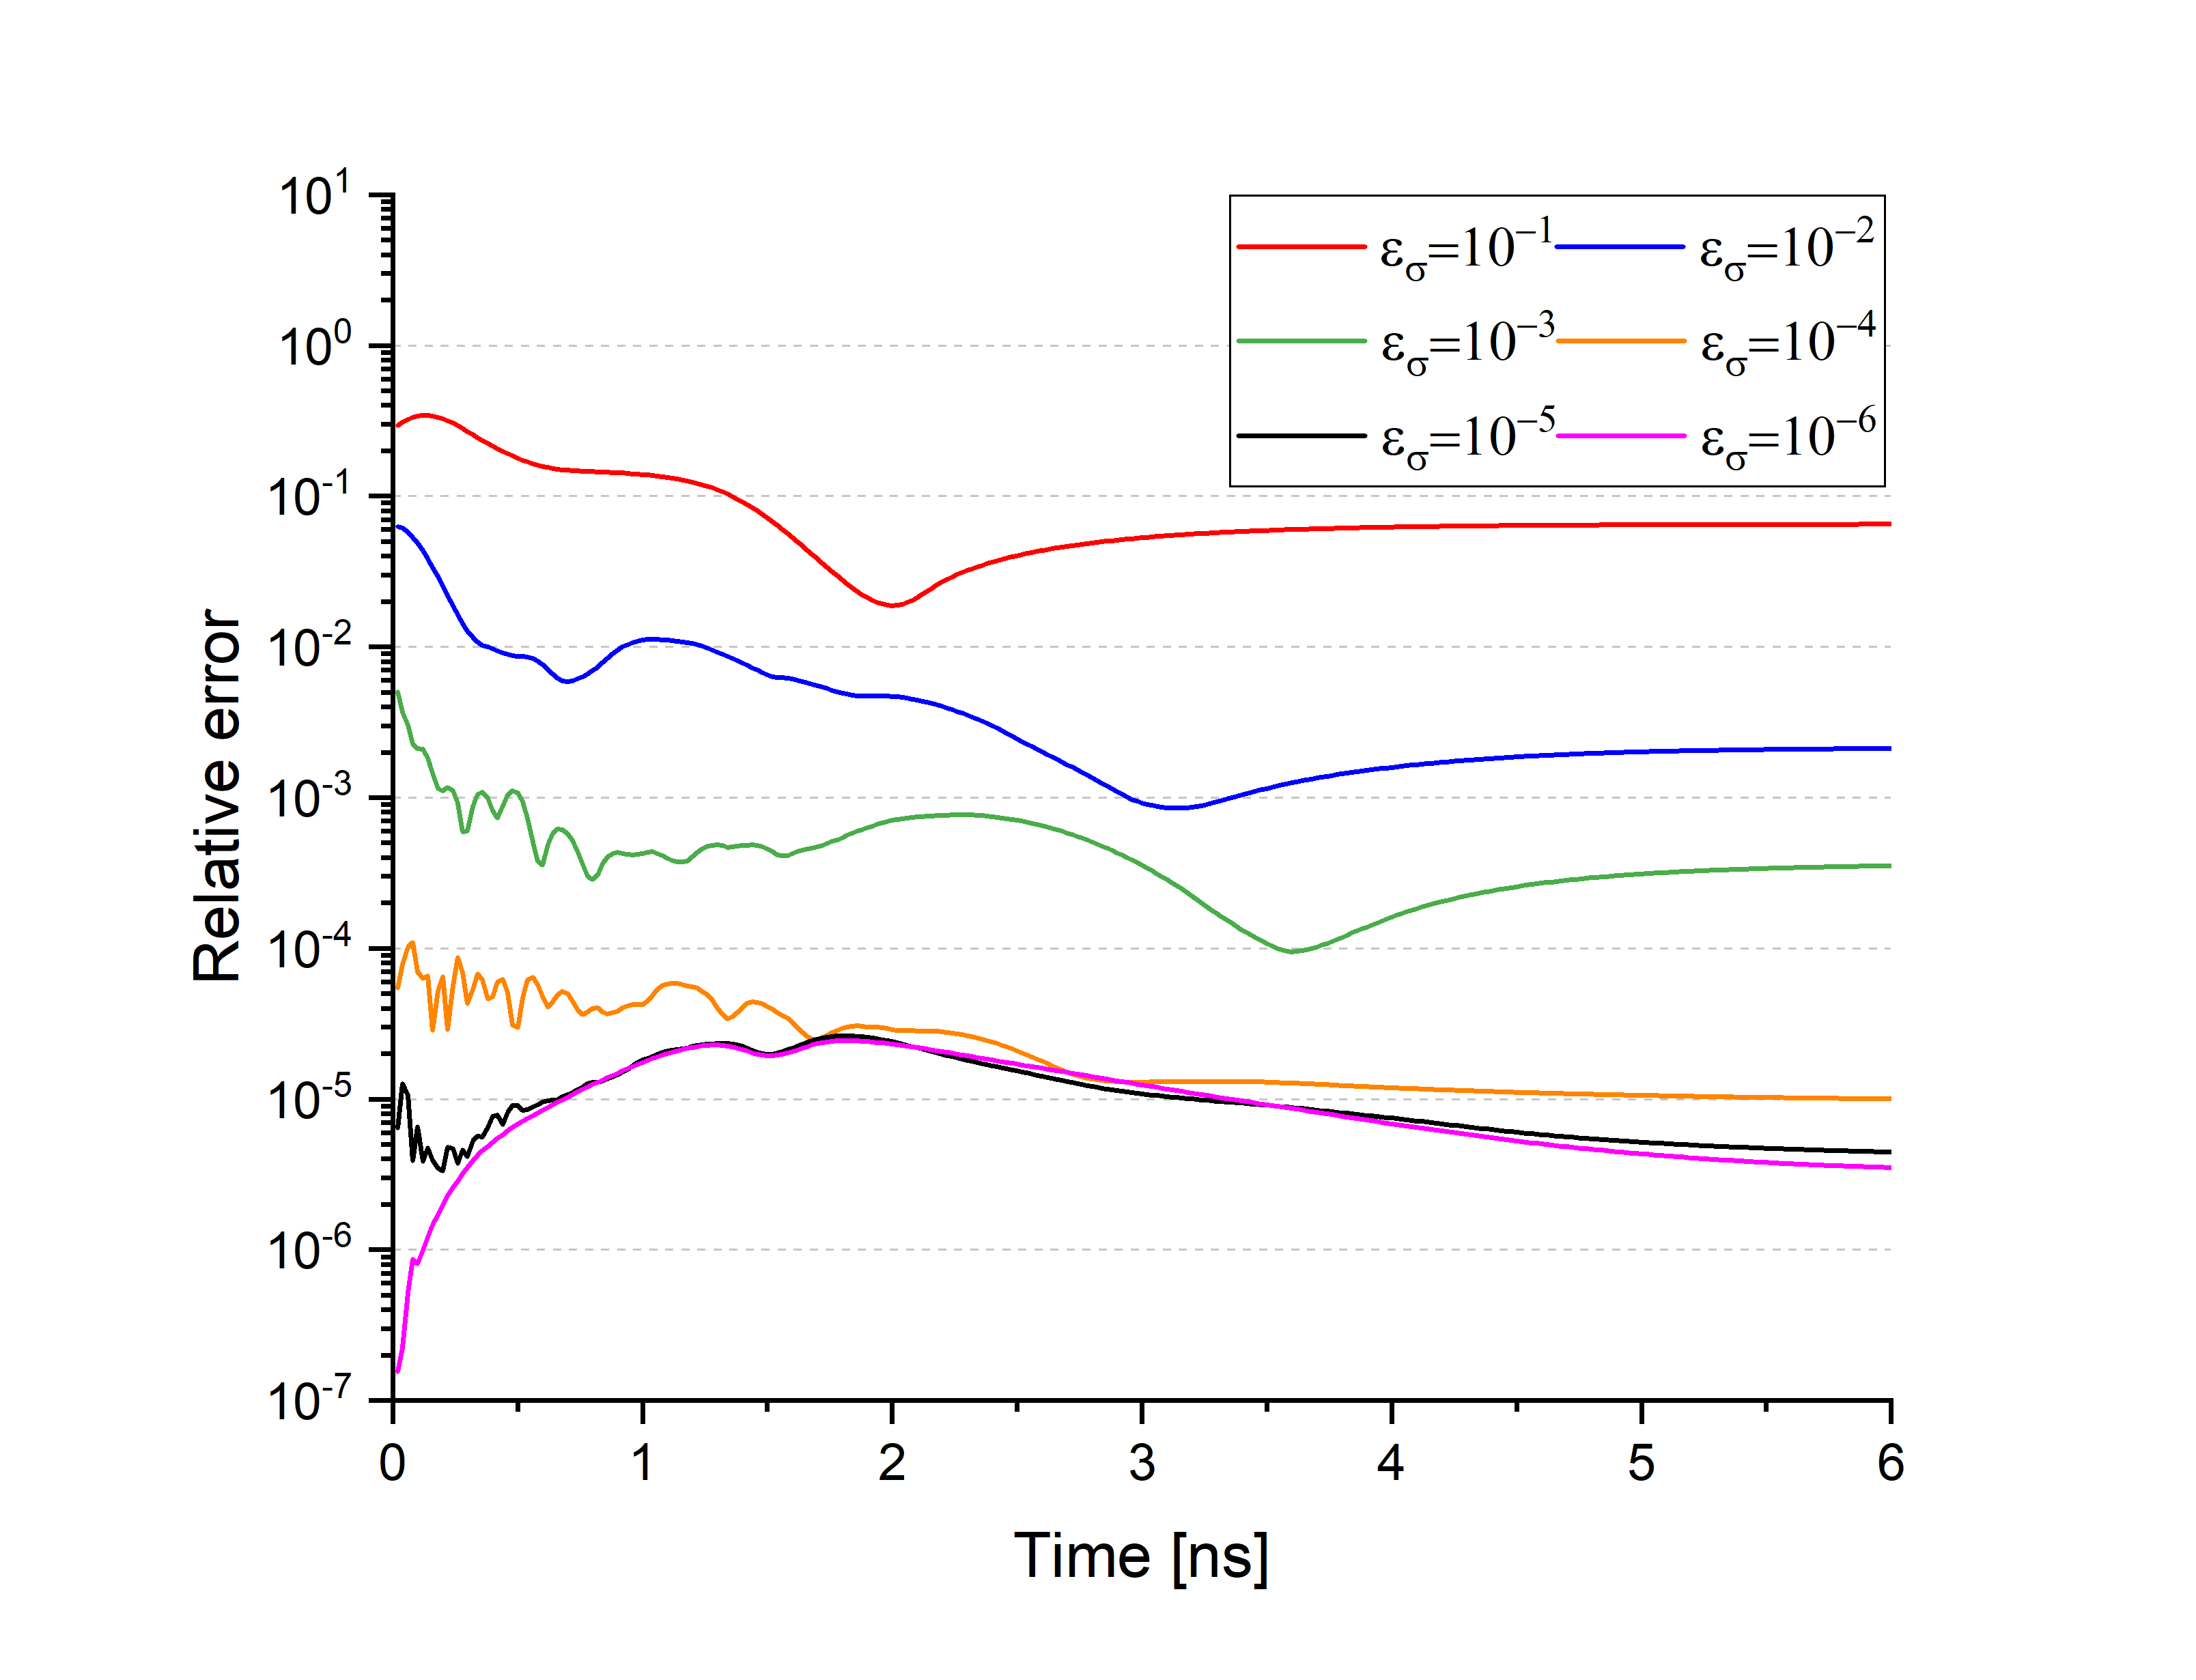
\includegraphics[width=0.5\textwidth]{MG_bc990-t002_qdf1000-980-t002_Eavg_mlqd.png}}
		\caption{\label{fig:errors_bc_T=990}
			Relative error in the $L_1$-norm of the MLOQD-POD ROM solutions computed with $T_{in}~=~0.99$~KeV using base cases with $T_{in}^{\pr{1}}=1$ KeV  and $T_{in}^{\pr{2}}=0.98$ KeV. }
	\end{figure}

	\begin{figure}[ht!]
		\centering
		\subfloat[Temperature relative error \label{subfig:MG_bc980-t002_qdf1000-960-t002_Tavg_mlqd}]{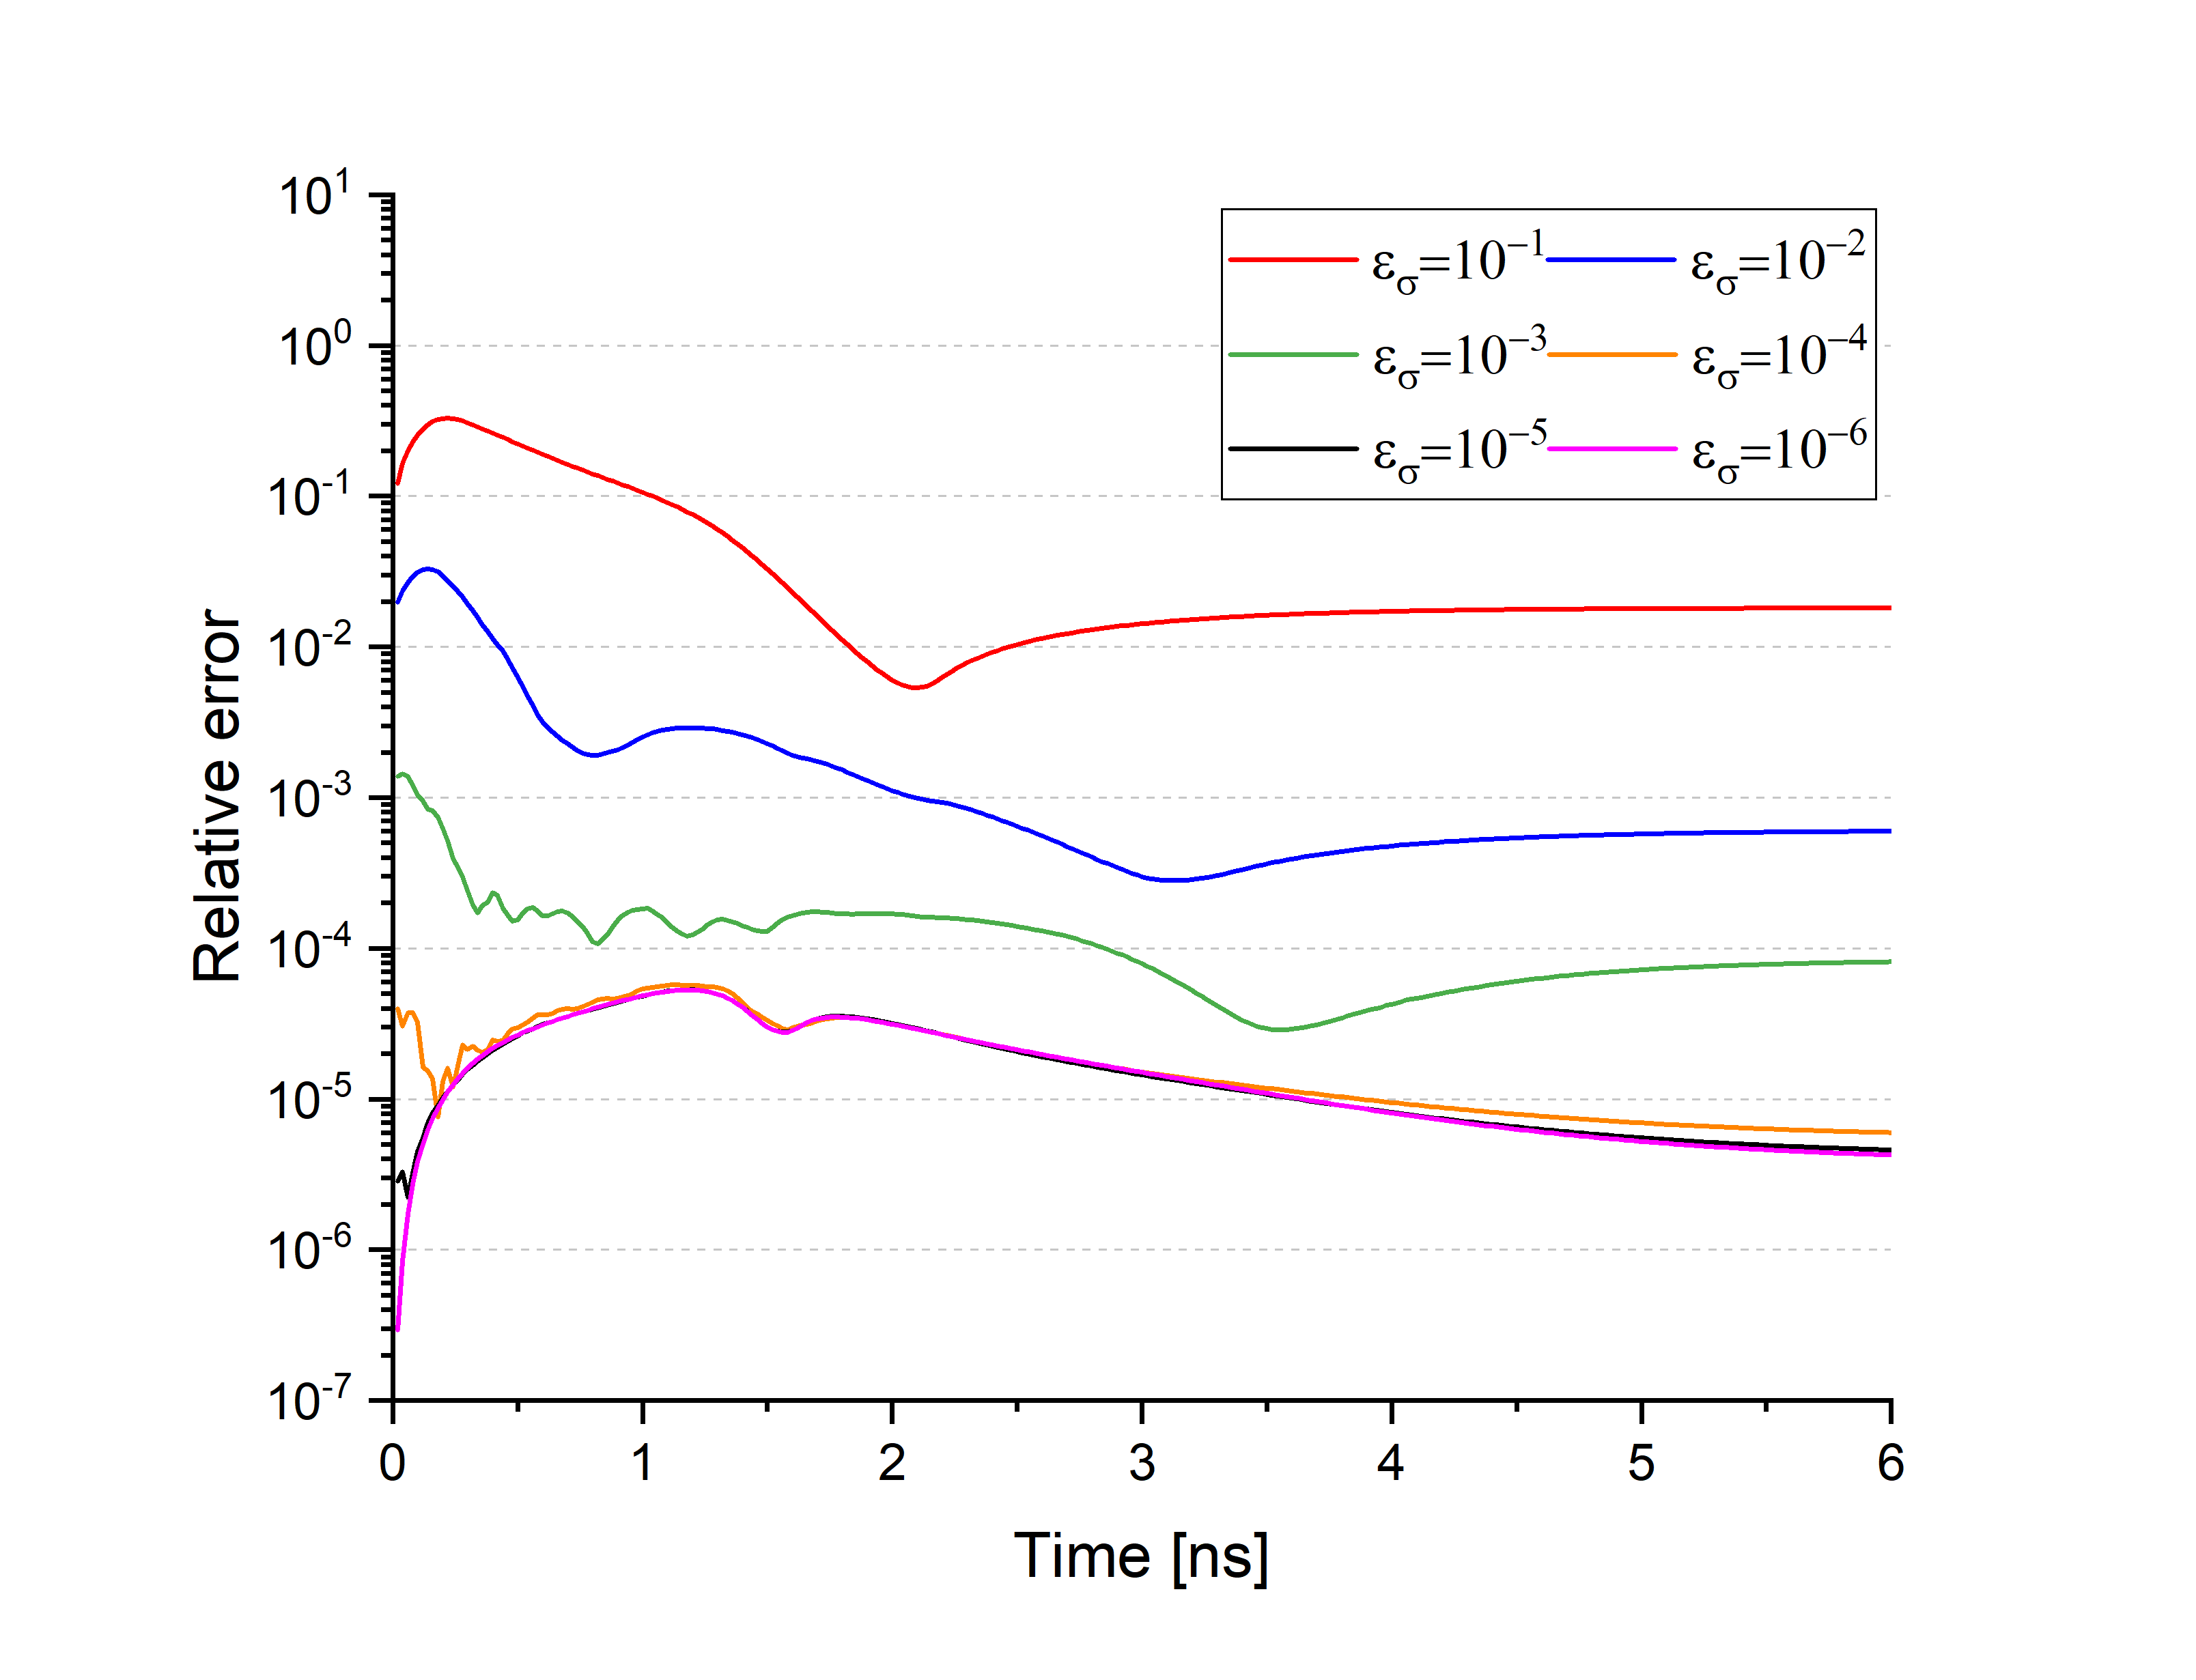
\includegraphics[width=0.5\textwidth]{MG_bc980-t002_qdf1000-960-t002_Tavg_mlqd.png}}
		\subfloat[Energy density relative error \label{subfig:MG_bc980-t002_qdf1000-960-t002_Eavg_mlqd}]{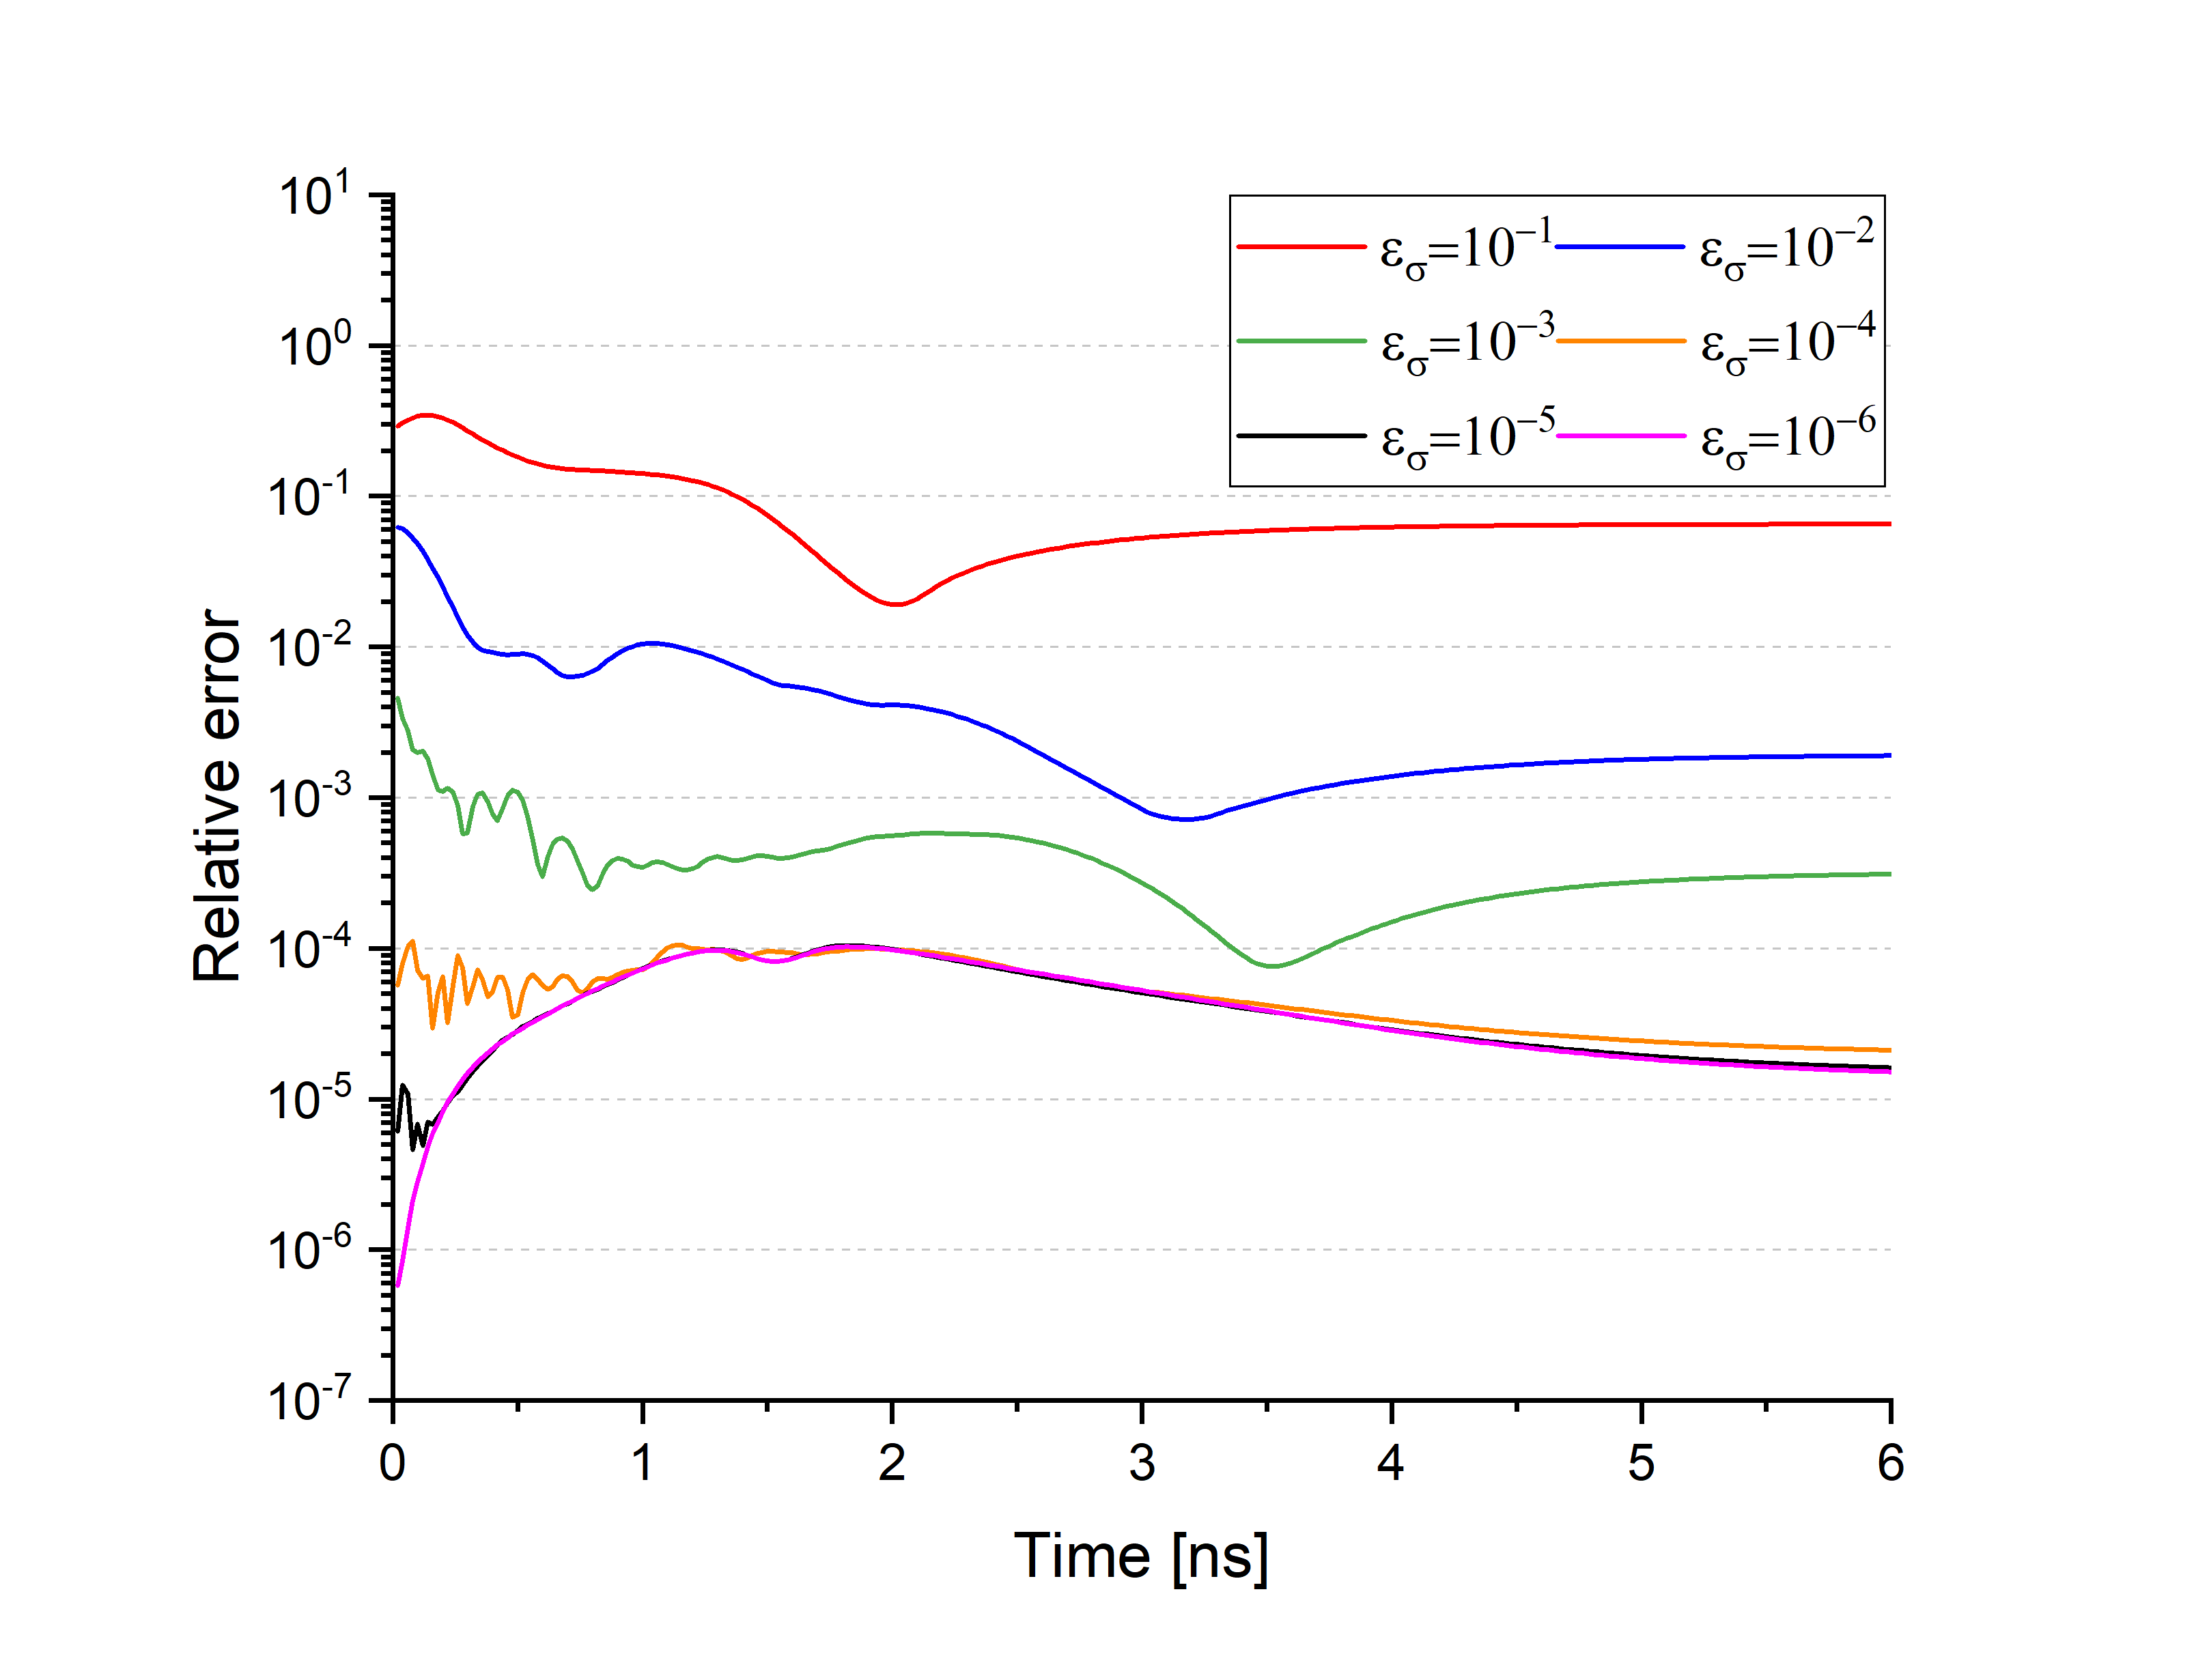
\includegraphics[width=0.5\textwidth]{MG_bc980-t002_qdf1000-960-t002_Eavg_mlqd.png}}
		\caption{\label{fig:errors_bc_T=980}
			Relative error in the $L_1$-norm of the MLOQD-POD ROM solutions computed with $T_{in}~=~0.98$~KeV using base cases with $T_{in}^{\pr{1}}=1$ KeV  and $T_{in}^{\pr{2}}=0.96$ KeV.}
	\end{figure}

	\begin{figure}[ht!]
		\centering
		\subfloat[Temperature relative error \label{subfig:MG_bc960-t002_qdf1000-920-t002_Tavg_mlqd}]{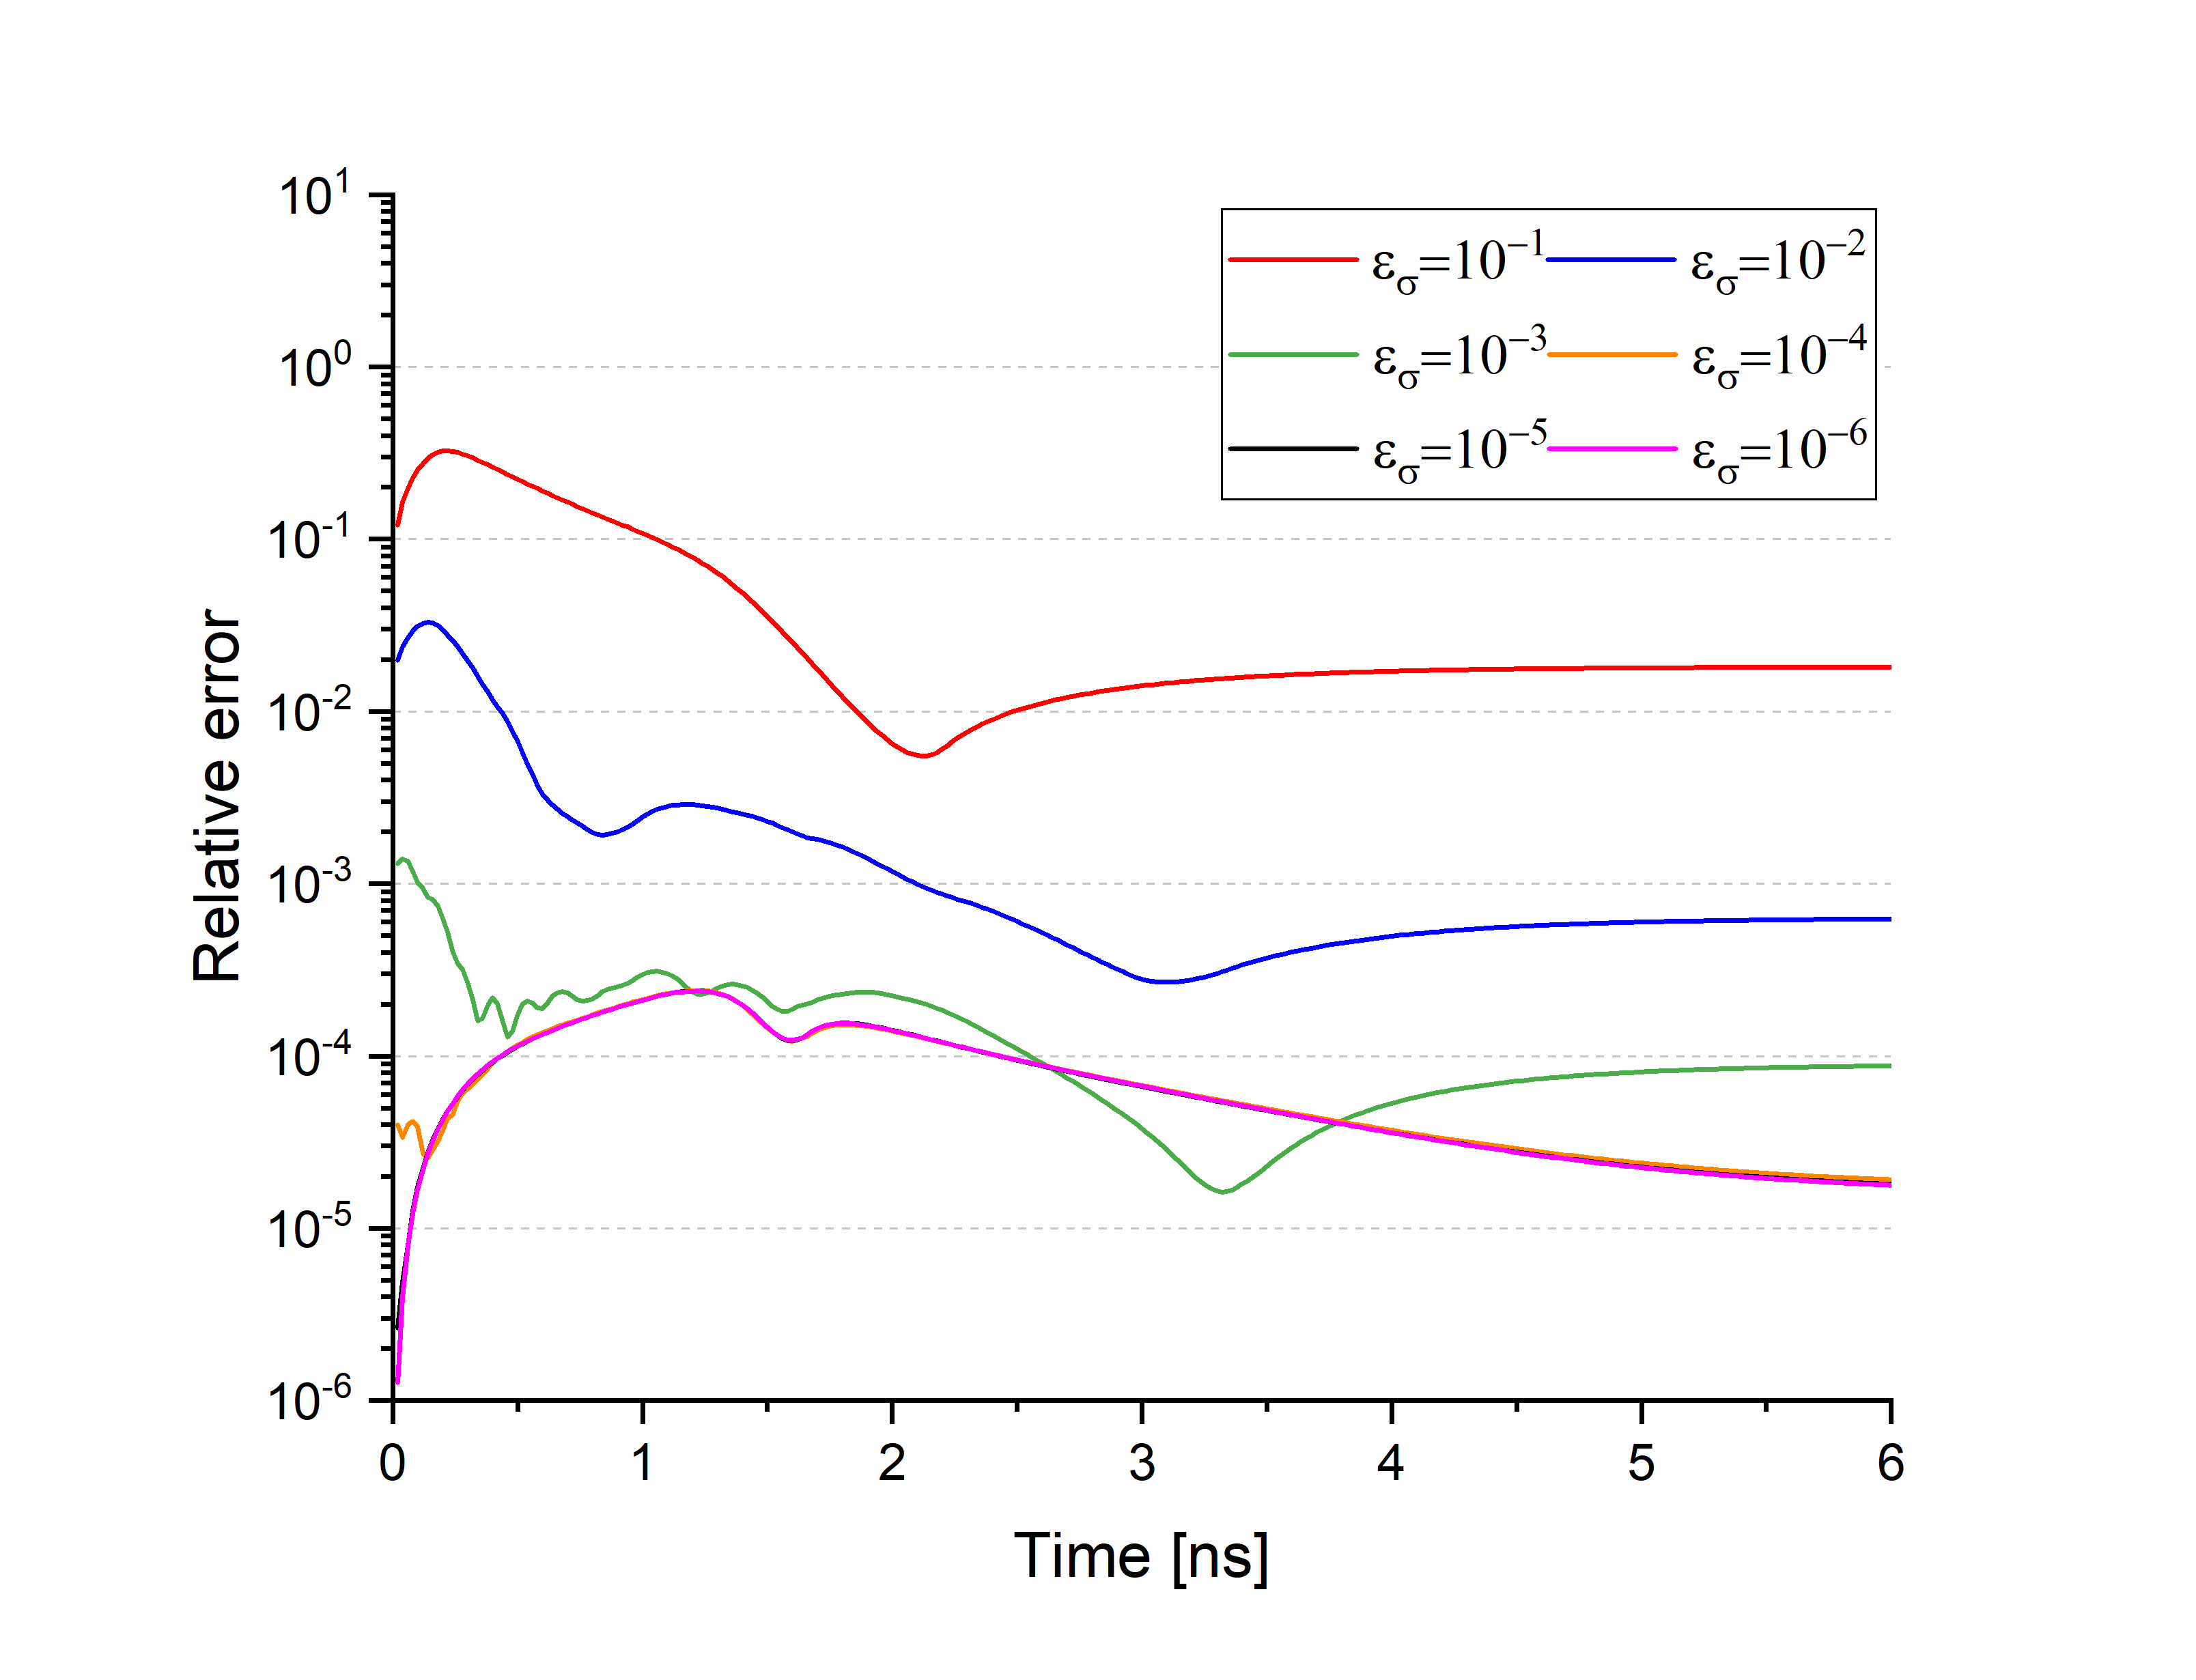
\includegraphics[width=0.5\textwidth]{MG_bc960-t002_qdf1000-920-t002_Tavg_mlqd.png}}
		\subfloat[Energy density relative error \label{subfig:MG_bc960-t002_qdf1000-920-t002_Eavg_mlqd}]{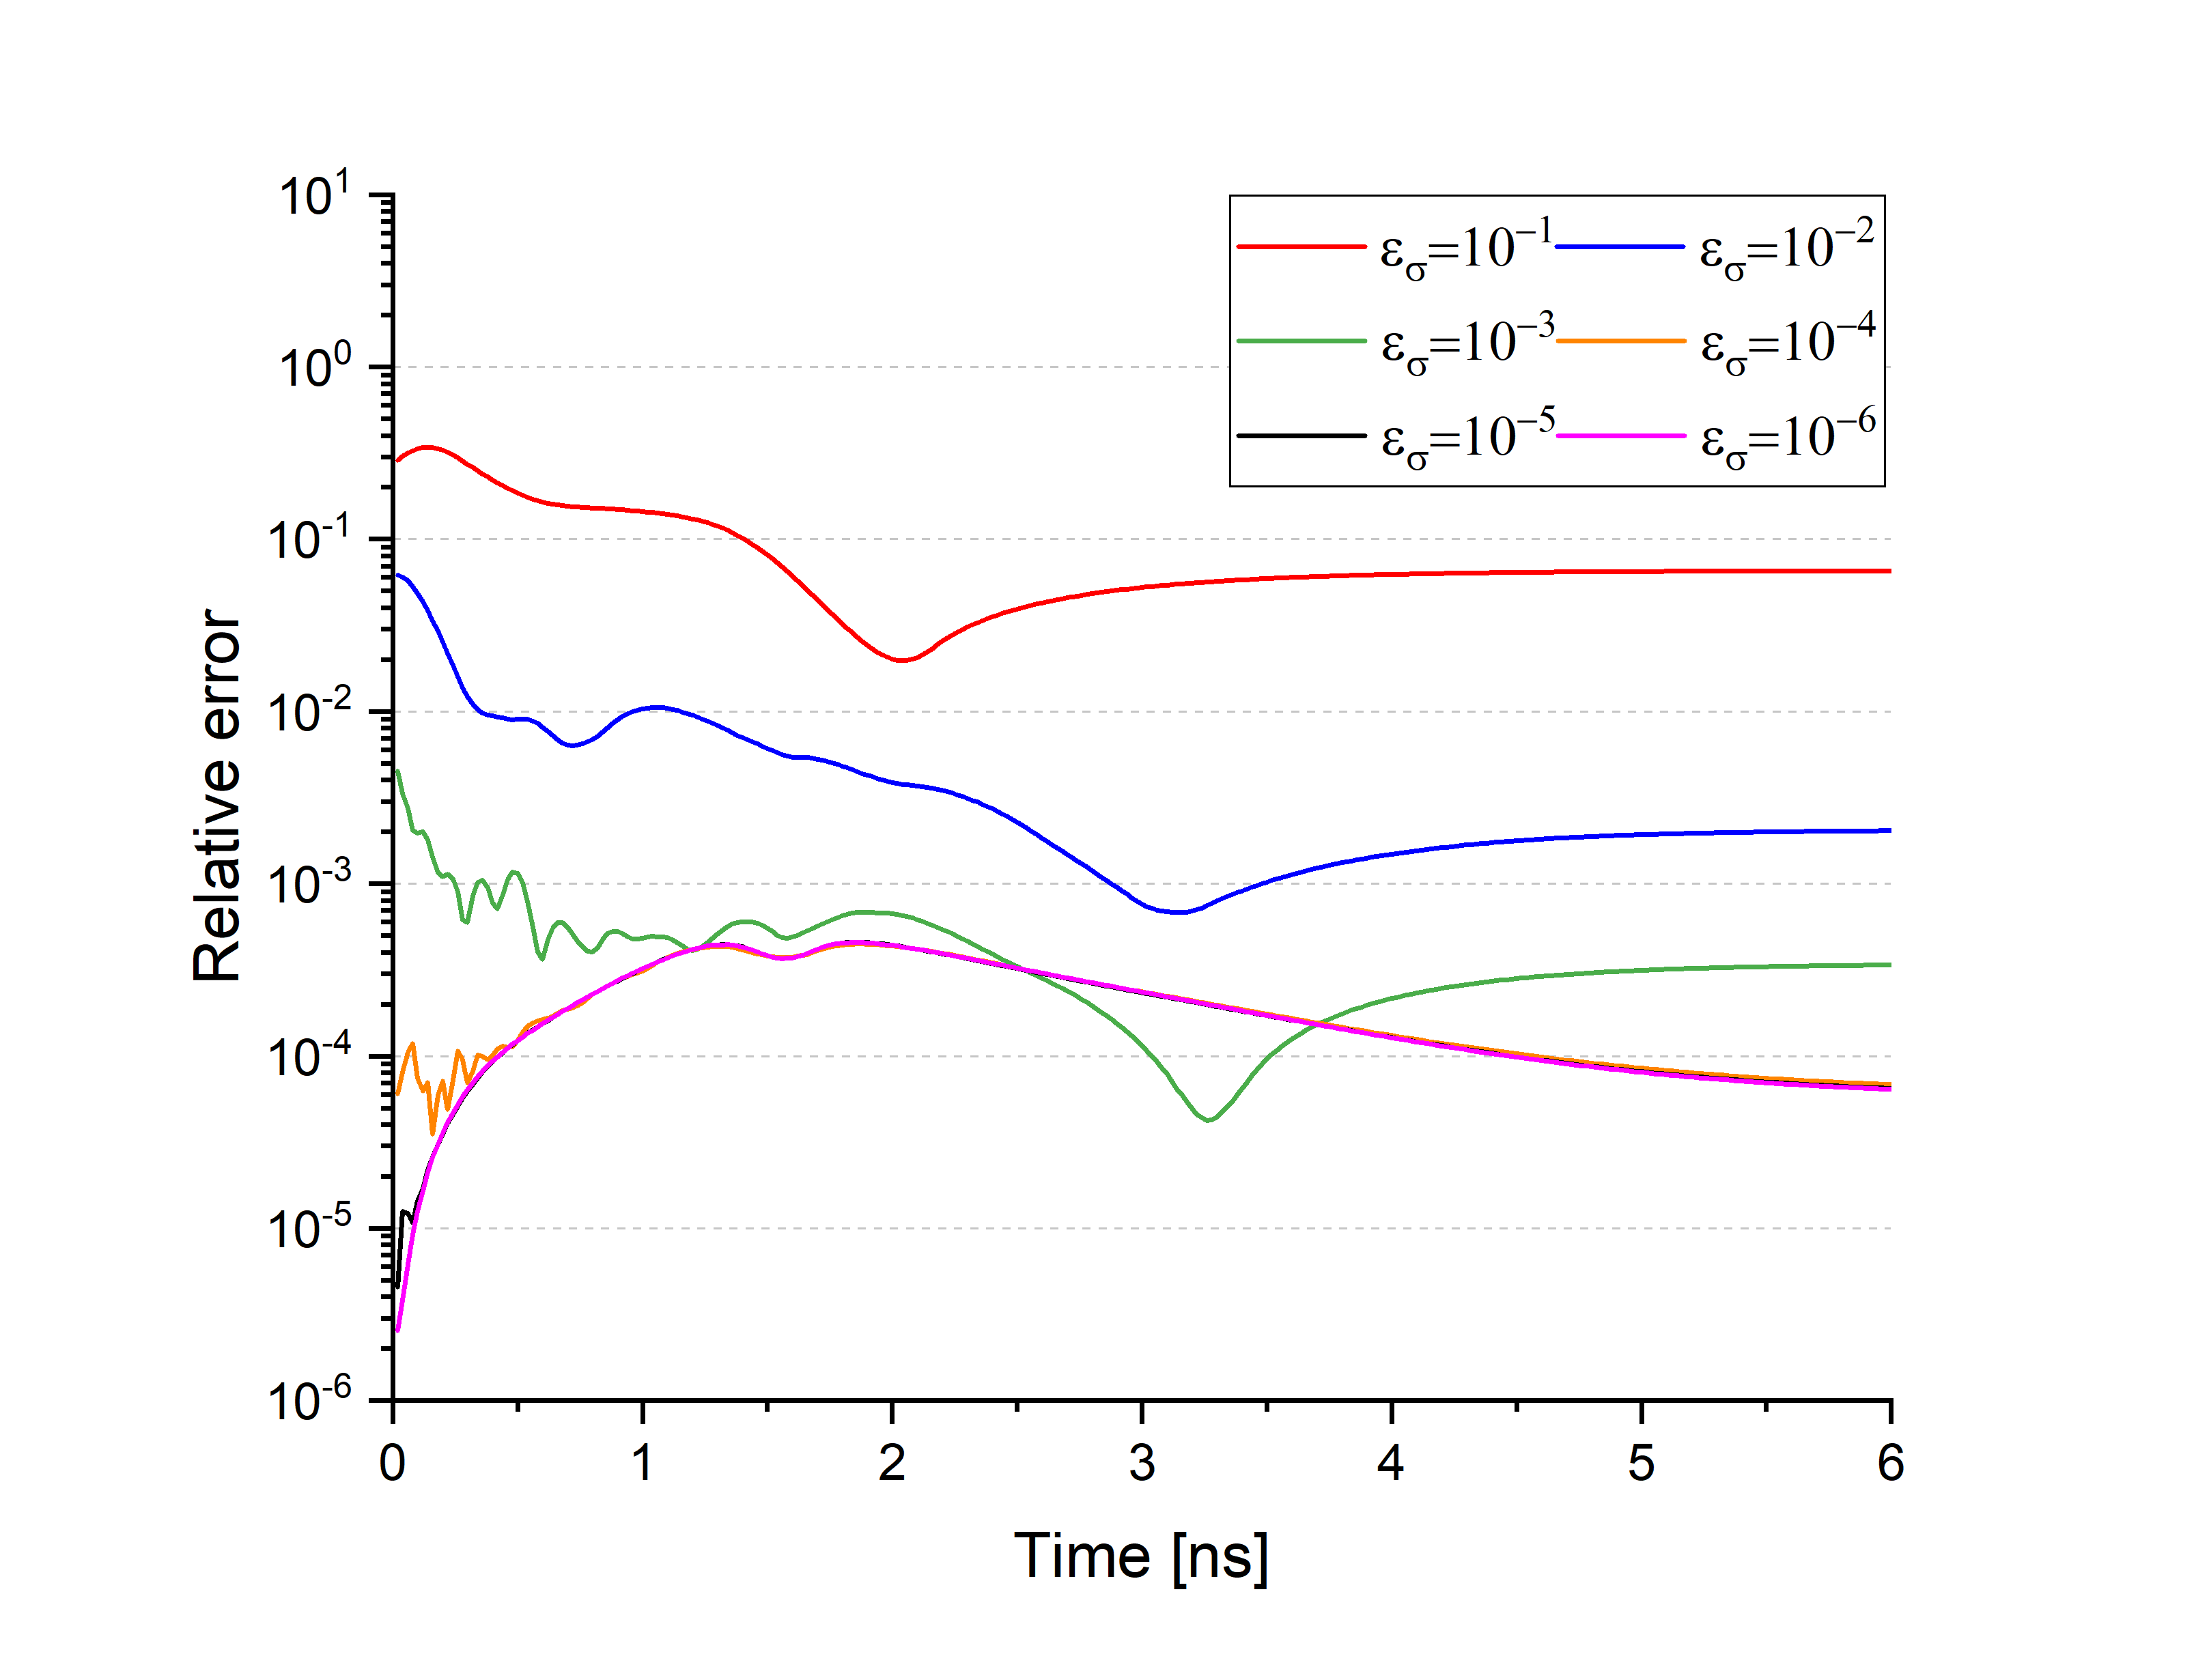
\includegraphics[width=0.5\textwidth]{MG_bc960-t002_qdf1000-920-t002_Eavg_mlqd.png}}
		\caption{\label{fig:errors_bc_T=960}
			Relative error in the $L_1$-norm of the MLOQD-POD ROM solutions computed with $T_{in}~=~0.96$~KeV using base cases with $T_{in}^{\pr{1}}=1$ KeV  and $T_{in}^{\pr{2}}=0.92$ KeV.}
	\end{figure}

	\ind The two types of ROMs utilizing an incomplete database can be combined to create a parameterized ROM with respect to the temperature $T_{in}$ of incoming radiation at the left boundary that also employs a reduced time step relative to the used database. In this case the same databases as created for the parameterized ROM in $T_{in}$ are adopted, now also interpolated linearly between instants of time. The first model uses $T_{in}^{(1)}~=~1$~KeV and $T_{in}^{(2)}=0.98$ KeV. The second one is formed with  $T_{in}^{(1)}=1$ KeV and $T_{in}^{(2)}=0.96$ KeV. The third is formed with  $T_{in}^{(1)}=1$ KeV and $T_{in}^{(2)}=0.92$ KeV. The data is generated for $\Delta t = 2\times10^{-2}$ ns. Figure \ref{fig:errors_bc_T=990_t001} shows the relative error in $L_1$-norm in the MLOQD-POD ROM solution  for $T_{in}=0.99$ KeV and $\Delta t = \! 1\! \times\! 10^{-2}$ ns computed by means of the first model with various values of $\varepsilon_{\sigma}$. Figure \ref{fig:errors_bc_T=980_t001} presents the relative error of the MLOQD-POD ROM solution for $T_{in}= 0.98$ KeV and $\Delta t = \! 1\! \times\! 10^{-2}$ ns obtained from the second model that is parameterized with a larger interval of $[T_{in}^{(1)},T_{in}^{(2)}]$. Figure \ref{fig:errors_bc_T=960_t001} presents the relative error of the MLOQD-POD ROM solution  for $T_{in}= 0.96$ KeV and $\Delta t = \! 1\! \times\! 10^{-2}$ ns obtained from the third model that is parameterized with the largest interval of  $[T_{in}^{(1)},T_{in}^{(2)}]$. The reference MLQD solution is recomputed for each $T_{in}$ at $\Delta t = \! 1\! \times\! 10^{-2}$ ns to find relative errors. The errors shown in Figs. \ref{fig:errors_bc_T=990_t001} - \ref{fig:errors_bc_T=960_t001} are very similar to Fig. \ref{fig:errors_dt-0.01}, and the error only marginally changes as the distance $[T_{in}^{(1)},T_{in}^{(2)}]$ is increased. This result demonstrates that these ROMs are most limited in accuracy by the refinement of time step length relative to the database of QD factors.

	%=================================================================================
	% BOUNDARY CONDITION DATABASE ERRORS PLOT	
	\begin{figure}[ht!]
		\centering
		\subfloat[Temperature relative error \label{subfig:MG_bc990-t001_qdf1000-980-t002_Tavg_mlqd}]{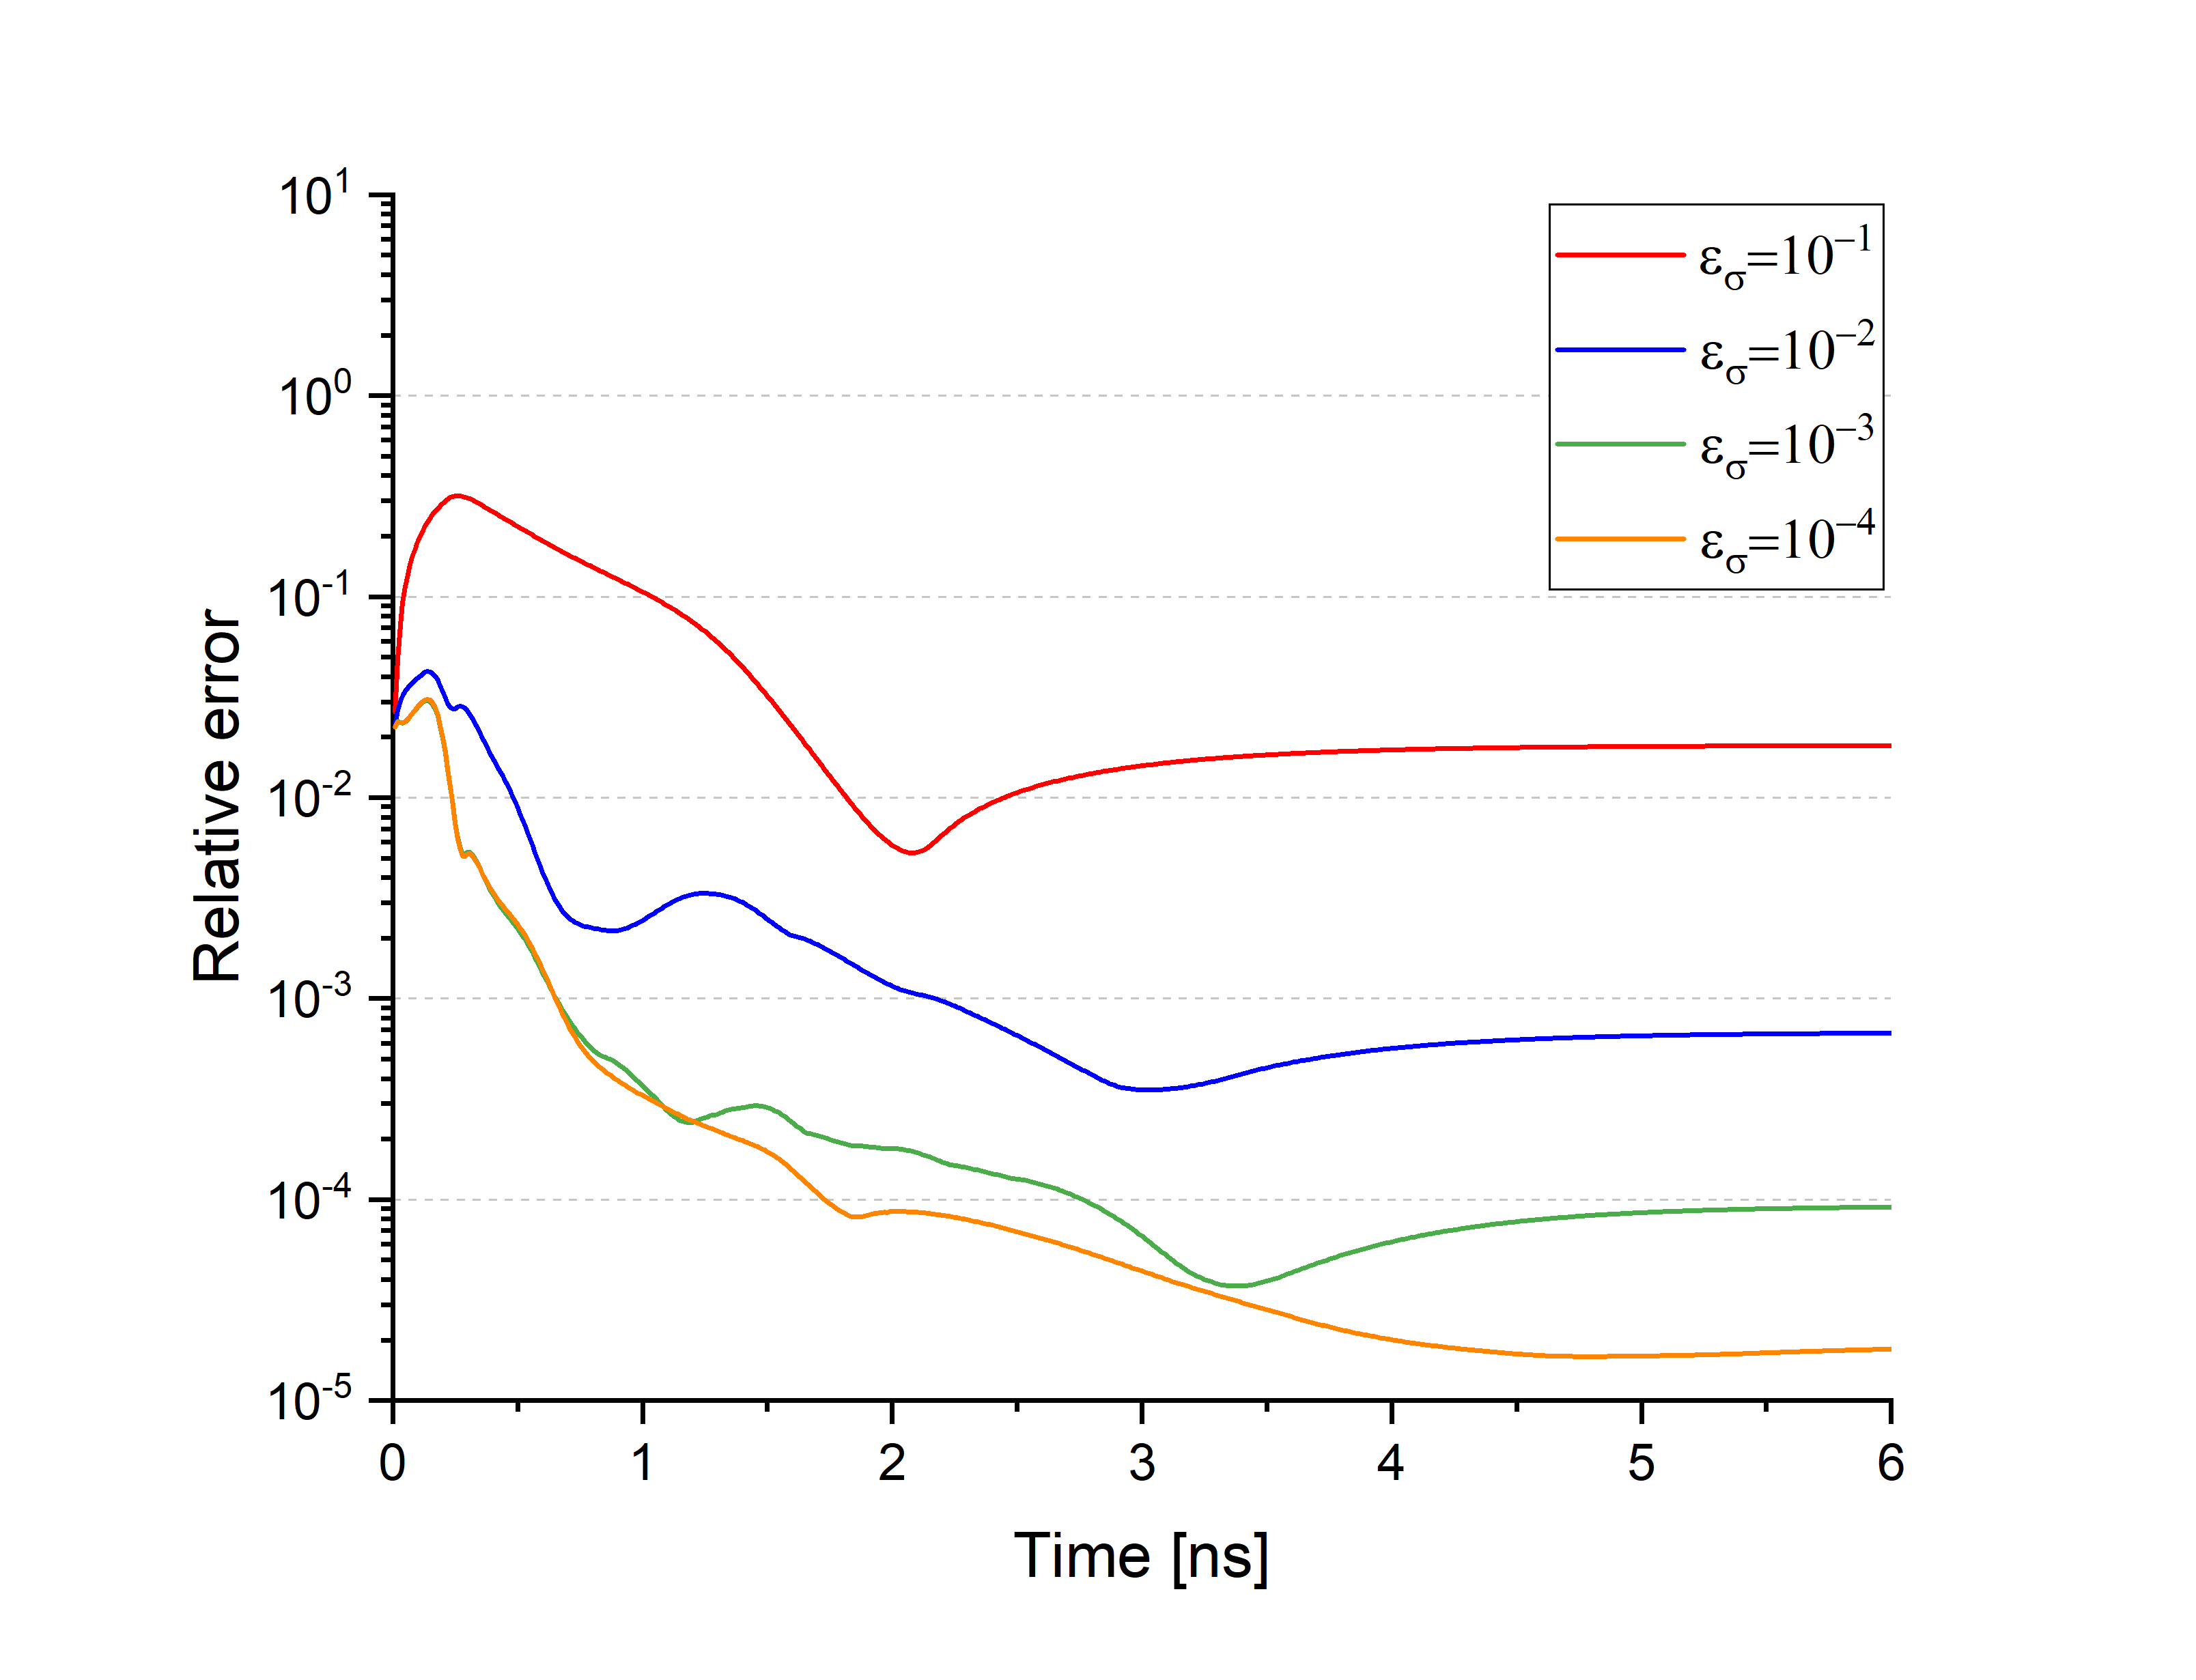
\includegraphics[width=0.5\textwidth]{MG_bc990-t001_qdf1000-980-t002_Tavg_mlqd.png}}
		\subfloat[Energy density relative error \label{subfig:MG_bc990-t001_qdf1000-980-t002_Eavg_mlqd}]{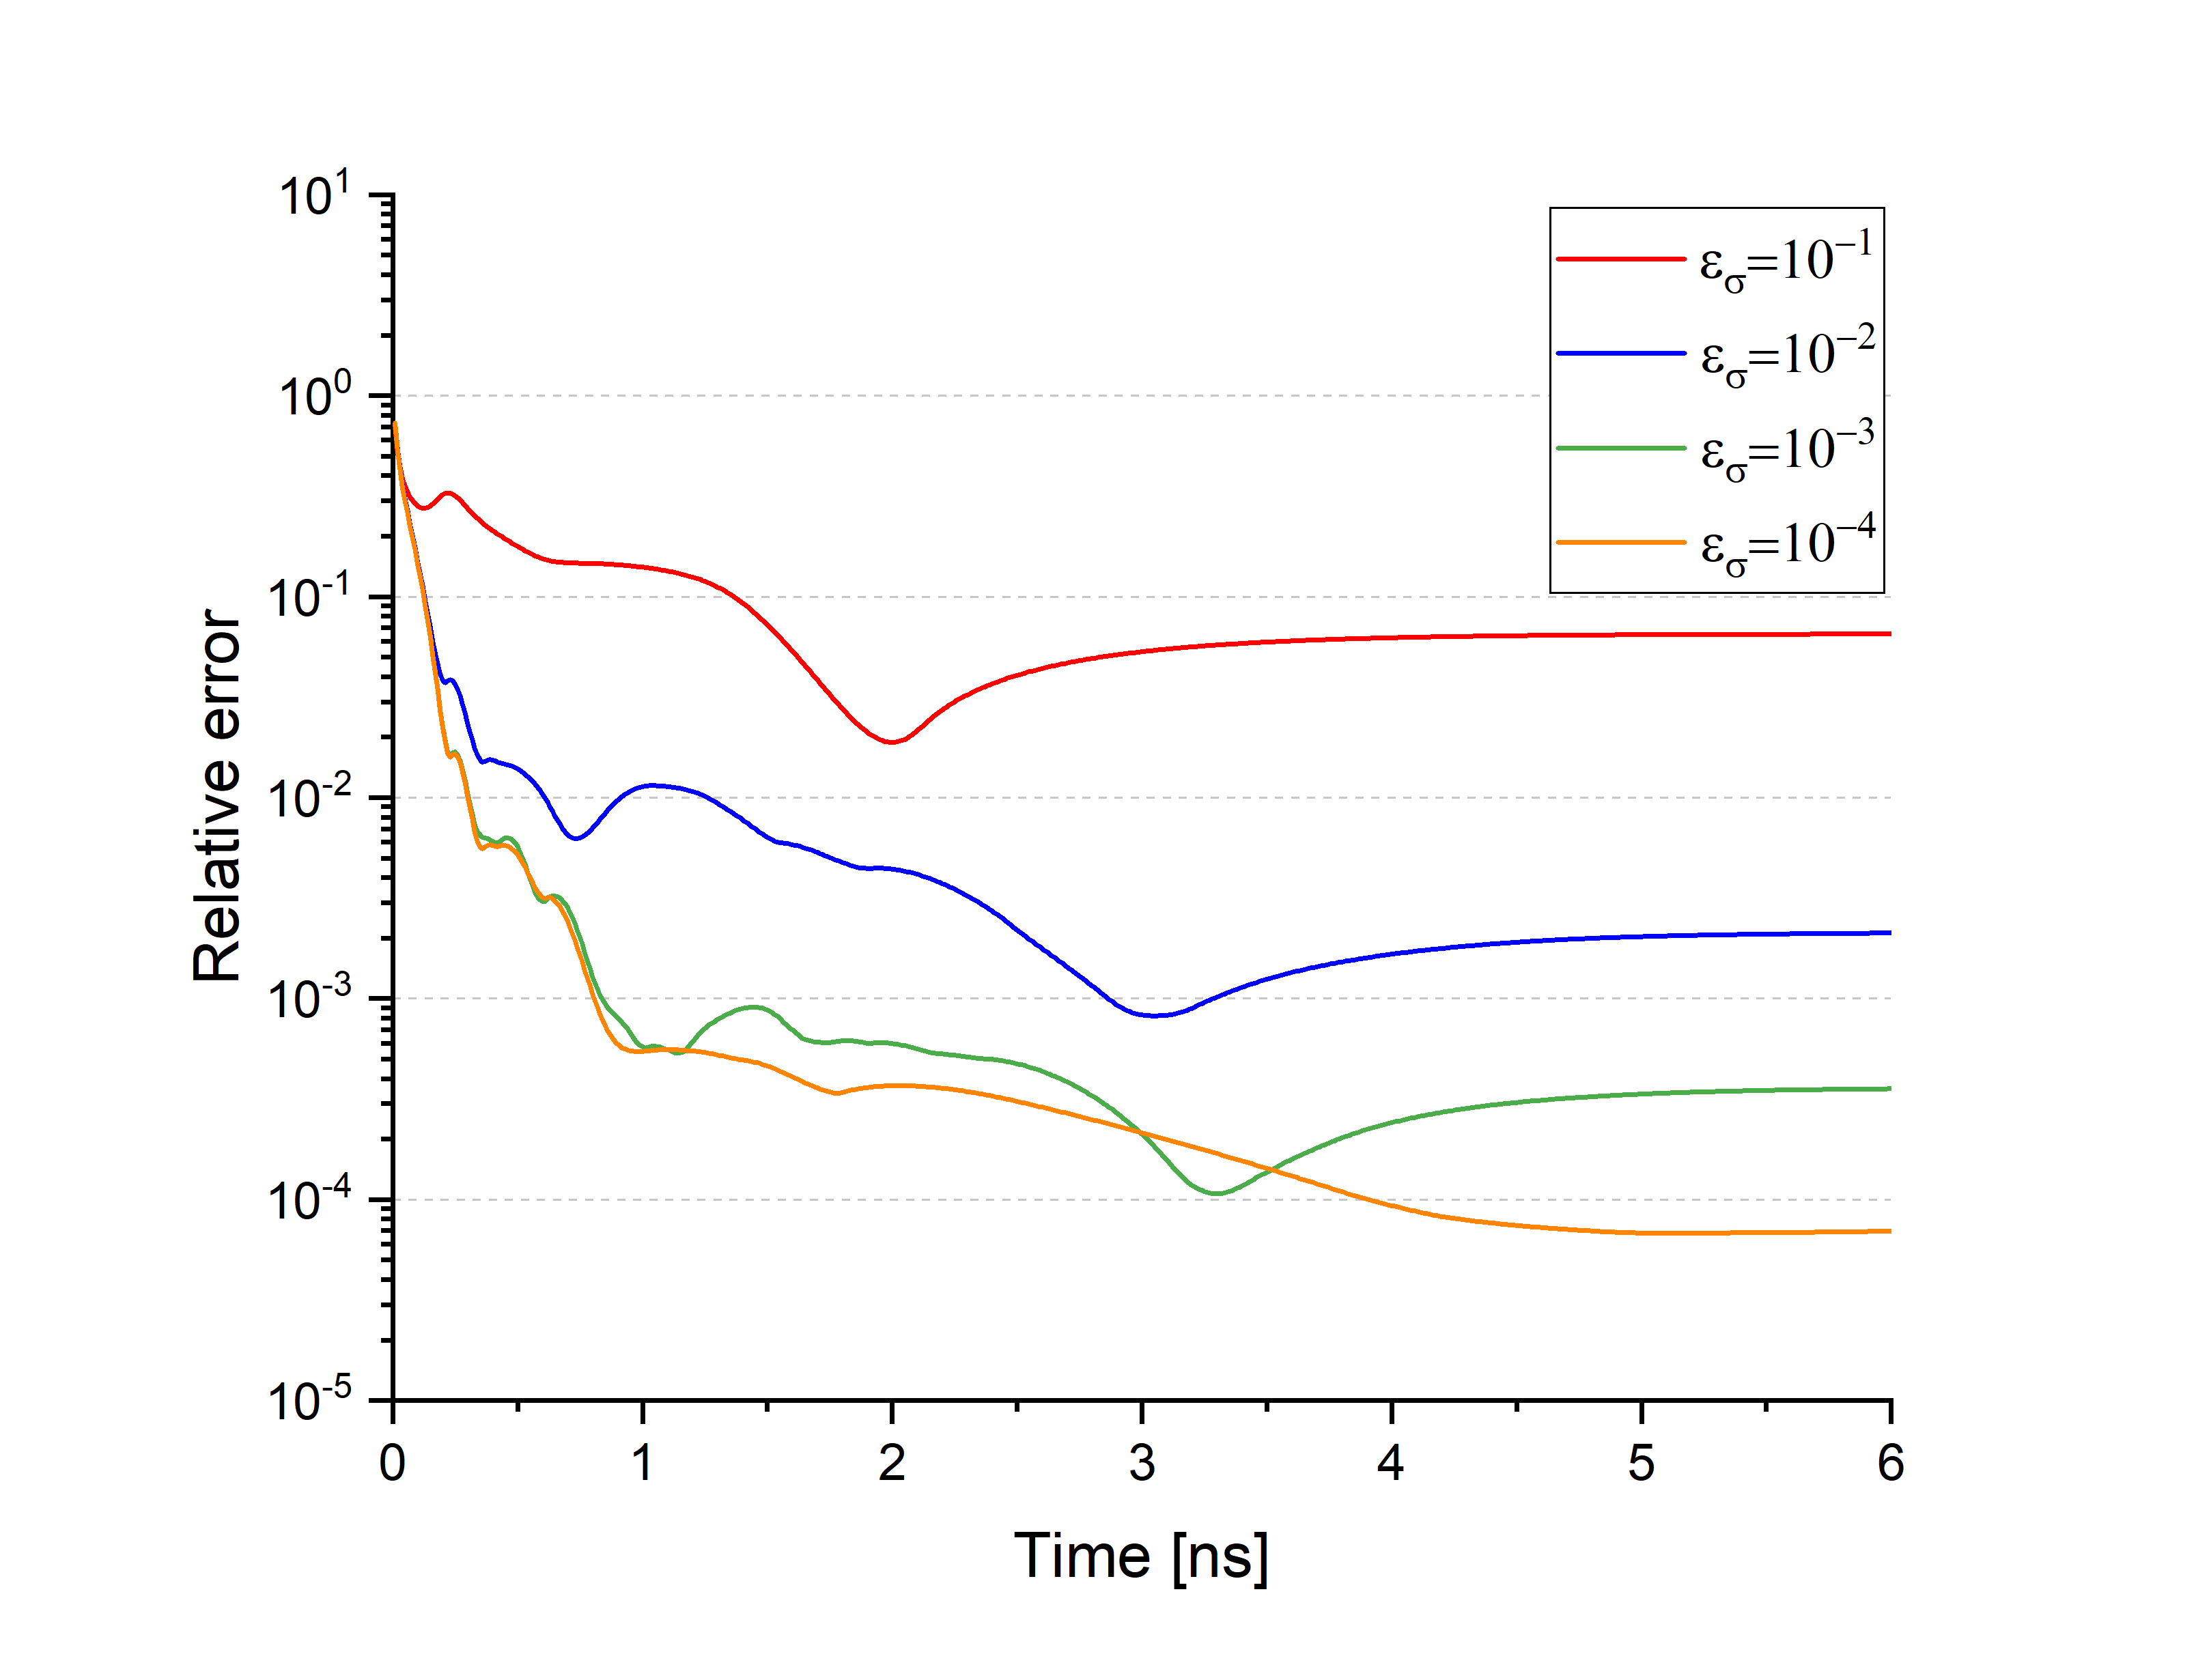
\includegraphics[width=0.5\textwidth]{MG_bc990-t001_qdf1000-980-t002_Eavg_mlqd.png}}
		\caption{\label{fig:errors_bc_T=990_t001}
			Relative error in the $L_1$-norm of the MLQD-POD solutions computed with $T_{in}~=~0.99$~KeV and $\Delta t\! =\! 1 \! \times \! 10^{-2}$~ns using base cases with $T_{in}^{\pr{1}}=1$ KeV  and $T_{in}^{\pr{2}}=0.98$ KeV and $\Delta t\! =\! 2 \! \times\!  10^{-2}$.}
	\end{figure}

	\begin{figure}[ht!]
		\centering
		\subfloat[Temperature relative error \label{subfig:MG_bc980-t001_qdf1000-960-t002_Tavg_mlqd}]{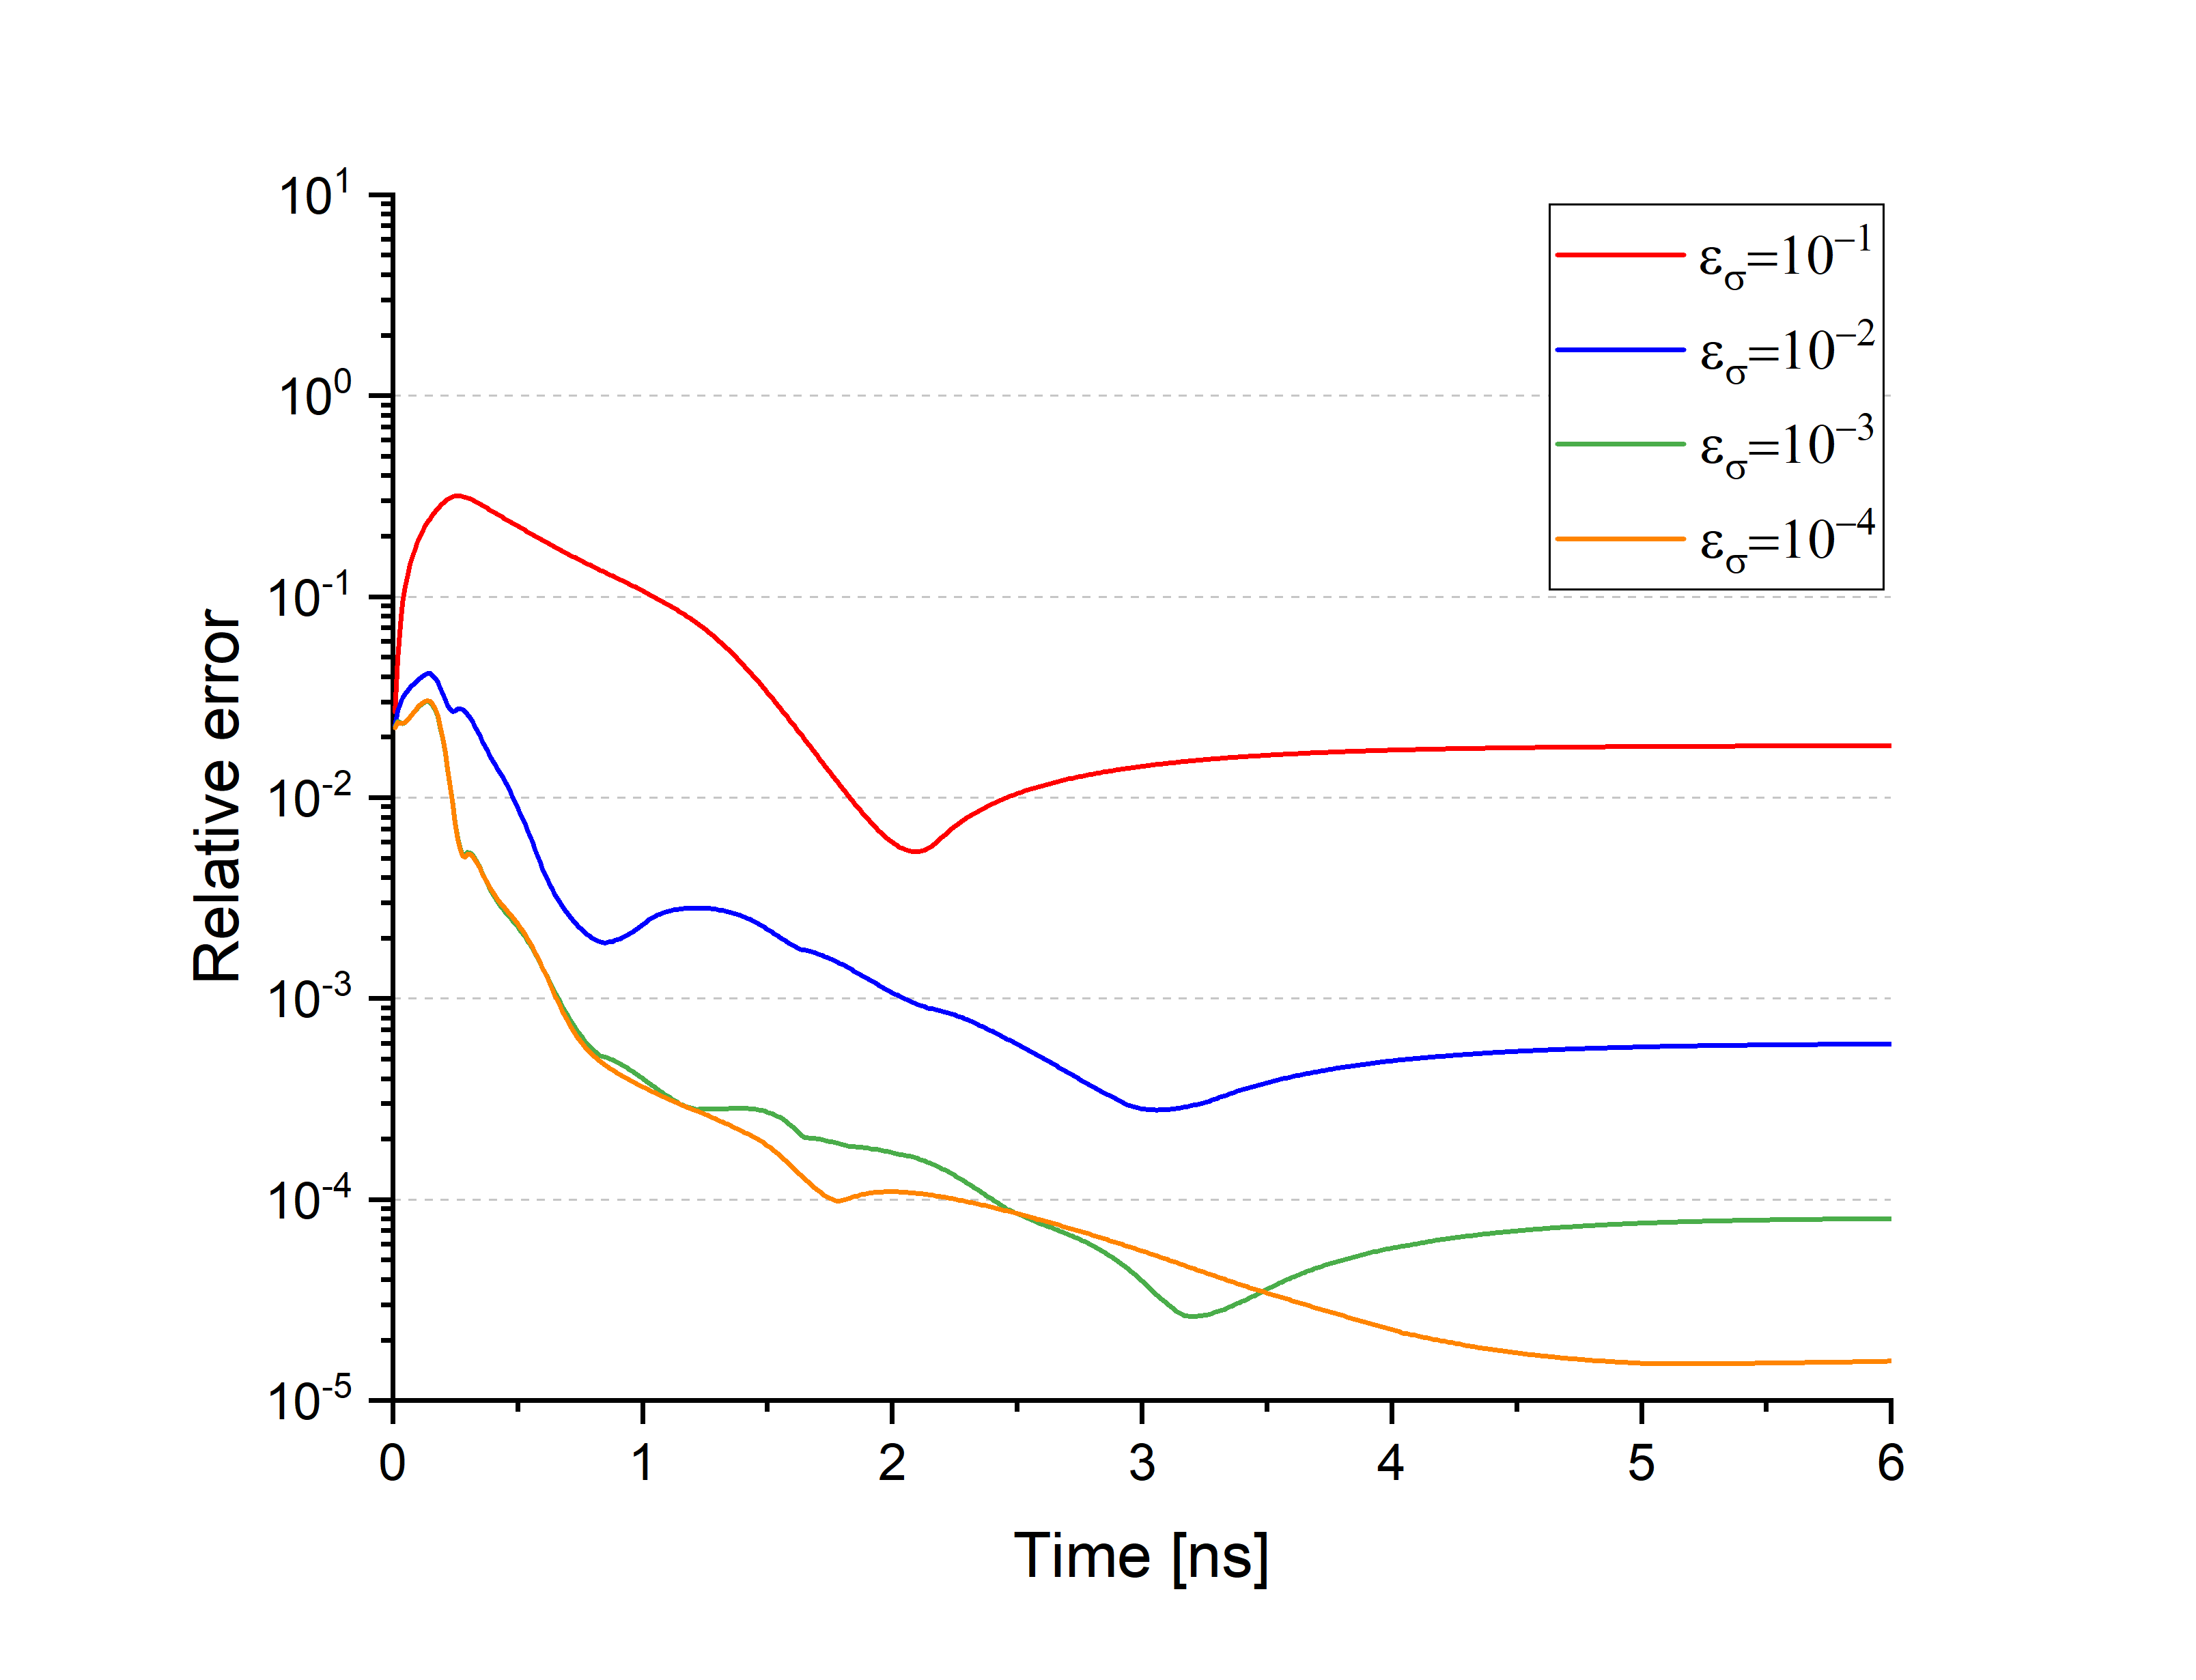
\includegraphics[width=0.5\textwidth]{MG_bc980-t001_qdf1000-960-t002_Tavg_mlqd.png}}
		\subfloat[Energy density relative error \label{subfig:MG_bc980-t001_qdf1000-960-t002_Eavg_mlqd}]{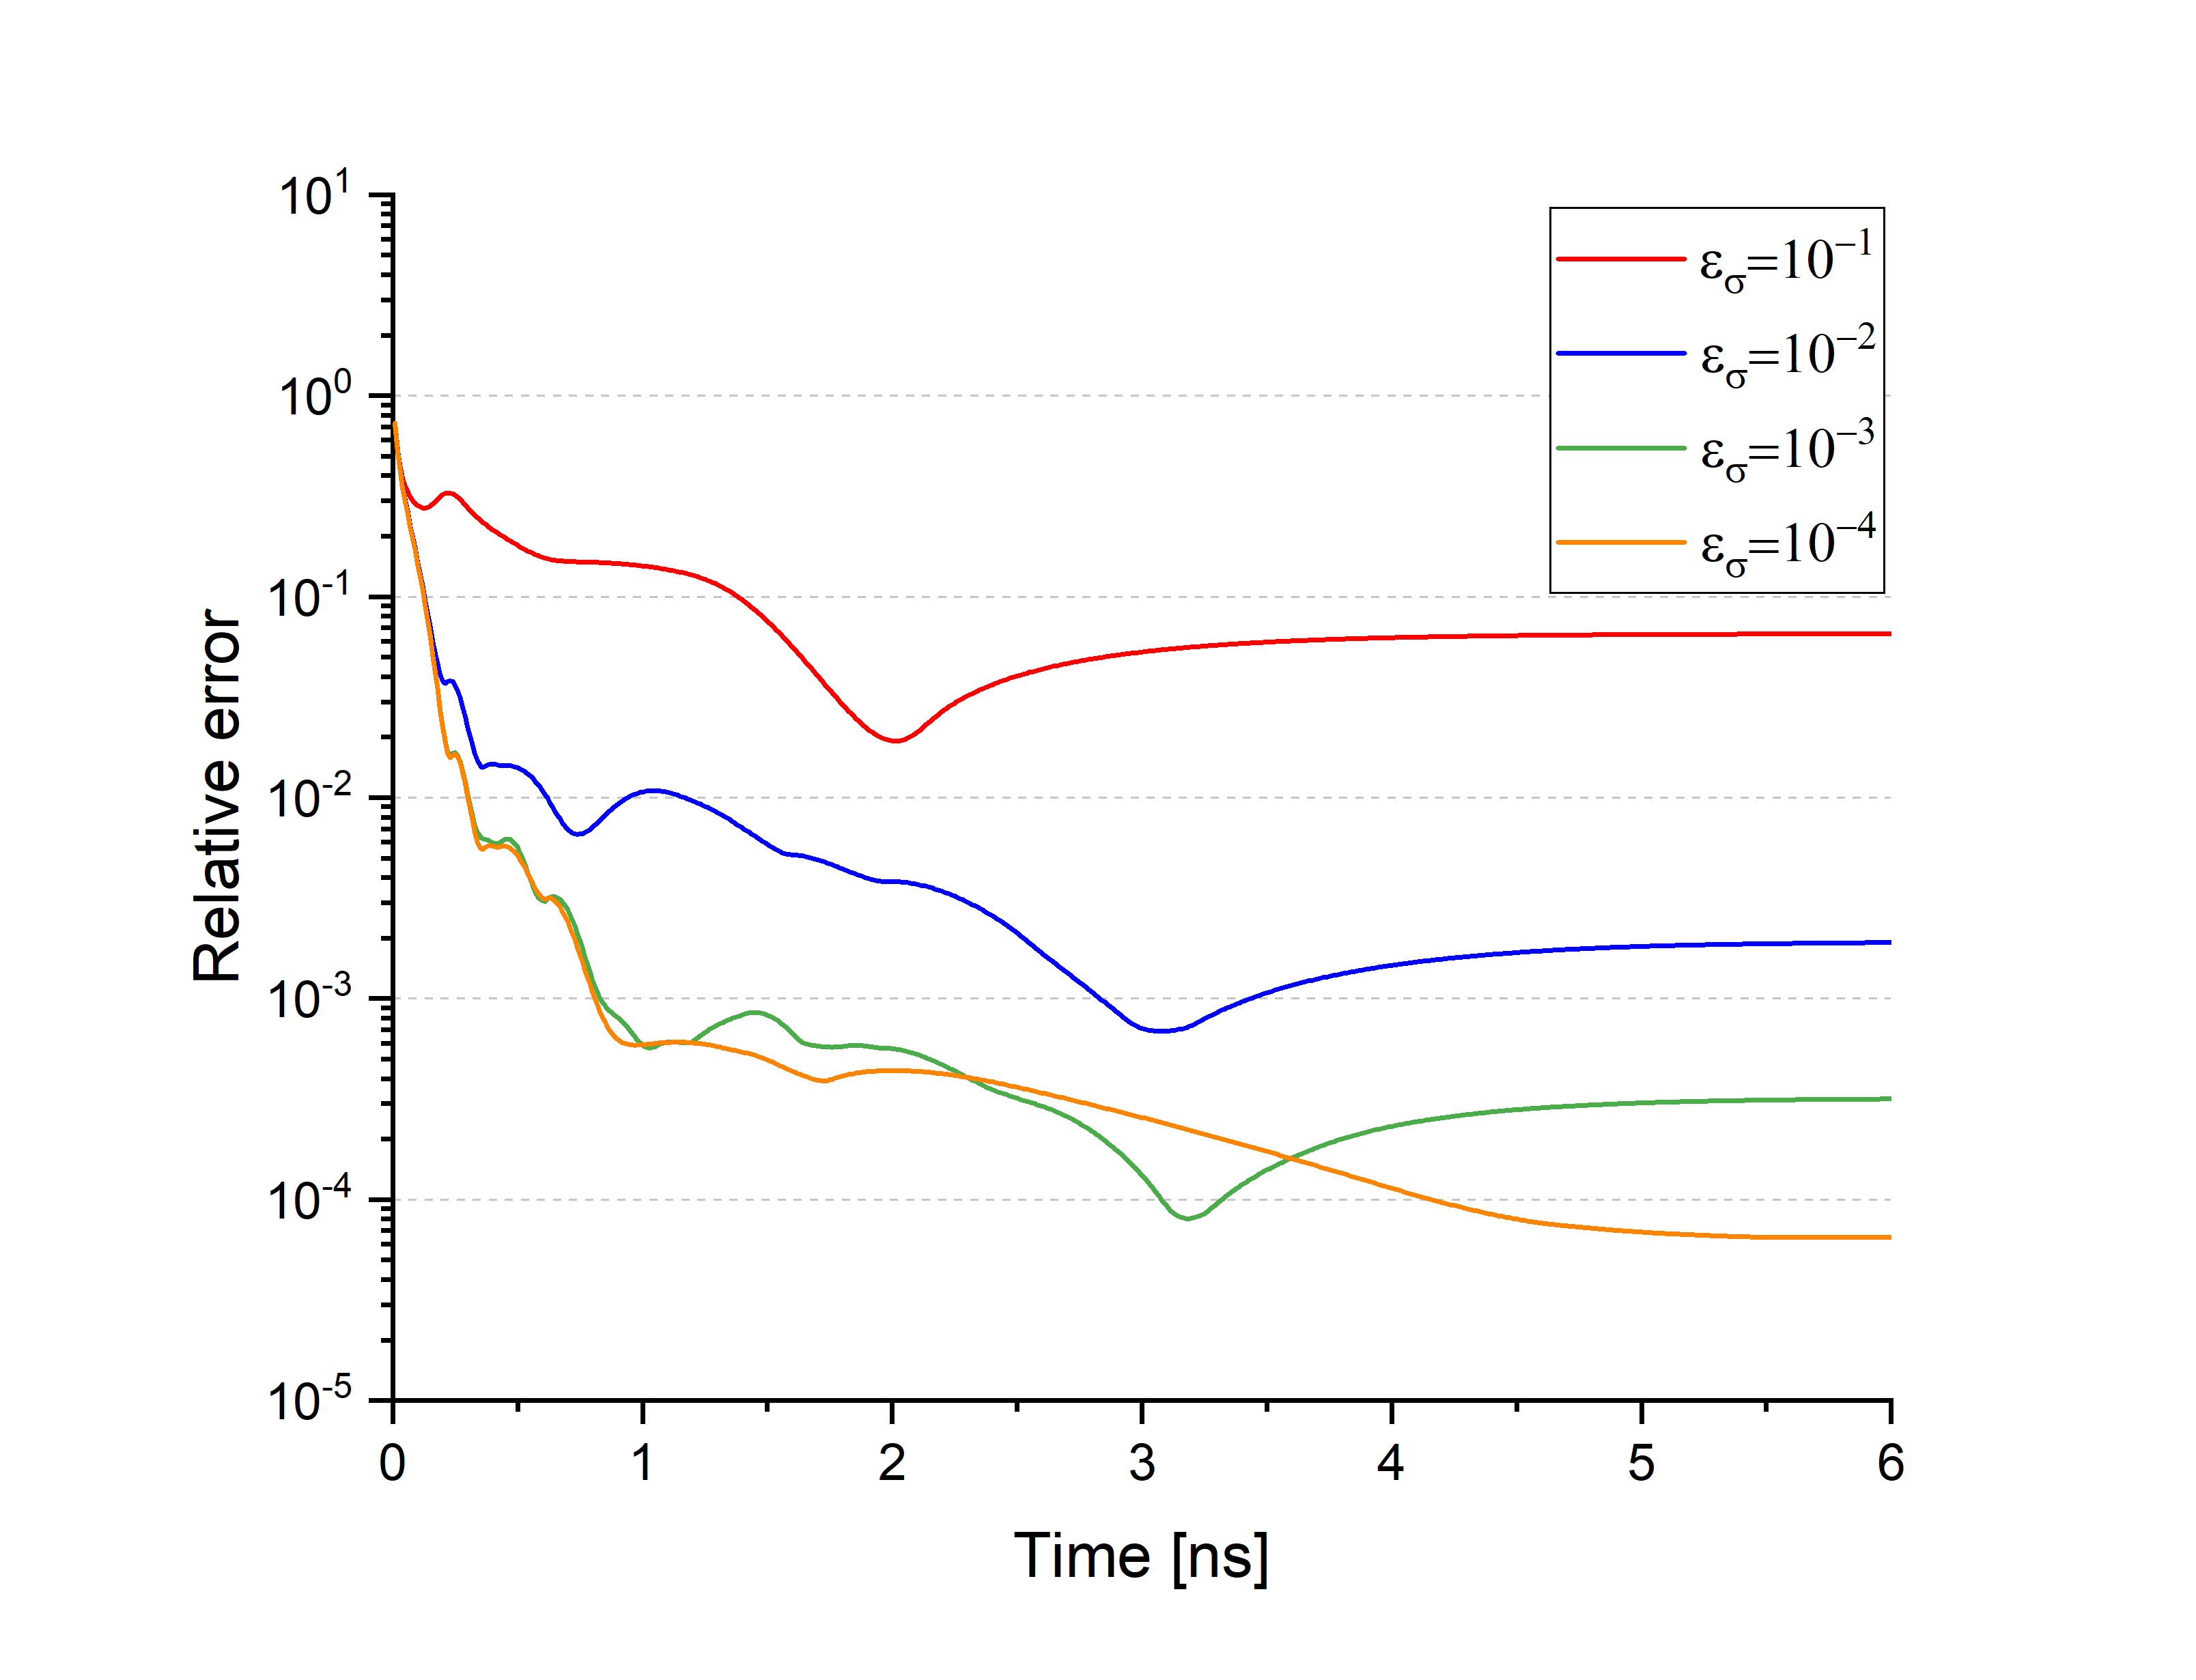
\includegraphics[width=0.5\textwidth]{MG_bc980-t001_qdf1000-960-t002_Eavg_mlqd.png}}
		\caption{\label{fig:errors_bc_T=980_t001}
			Relative error in the $L_1$-norm of the MLQD-POD solutions computed with $T_{in}~=~0.98$~KeV and $\Delta t\! =\! 1 \! \times \! 10^{-2}$~ns using base cases with $T_{in}^{\pr{1}}=1$ KeV  and $T_{in}^{\pr{2}}=0.96$ KeV and $\Delta t\! =\! 2 \! \times\!  10^{-2}$.}
	\end{figure}

	\begin{figure}[ht!]
		\centering
		\subfloat[Temperature relative error \label{subfig:MG_bc960-t001_qdf1000-920-t002_Tavg_mlqd}]{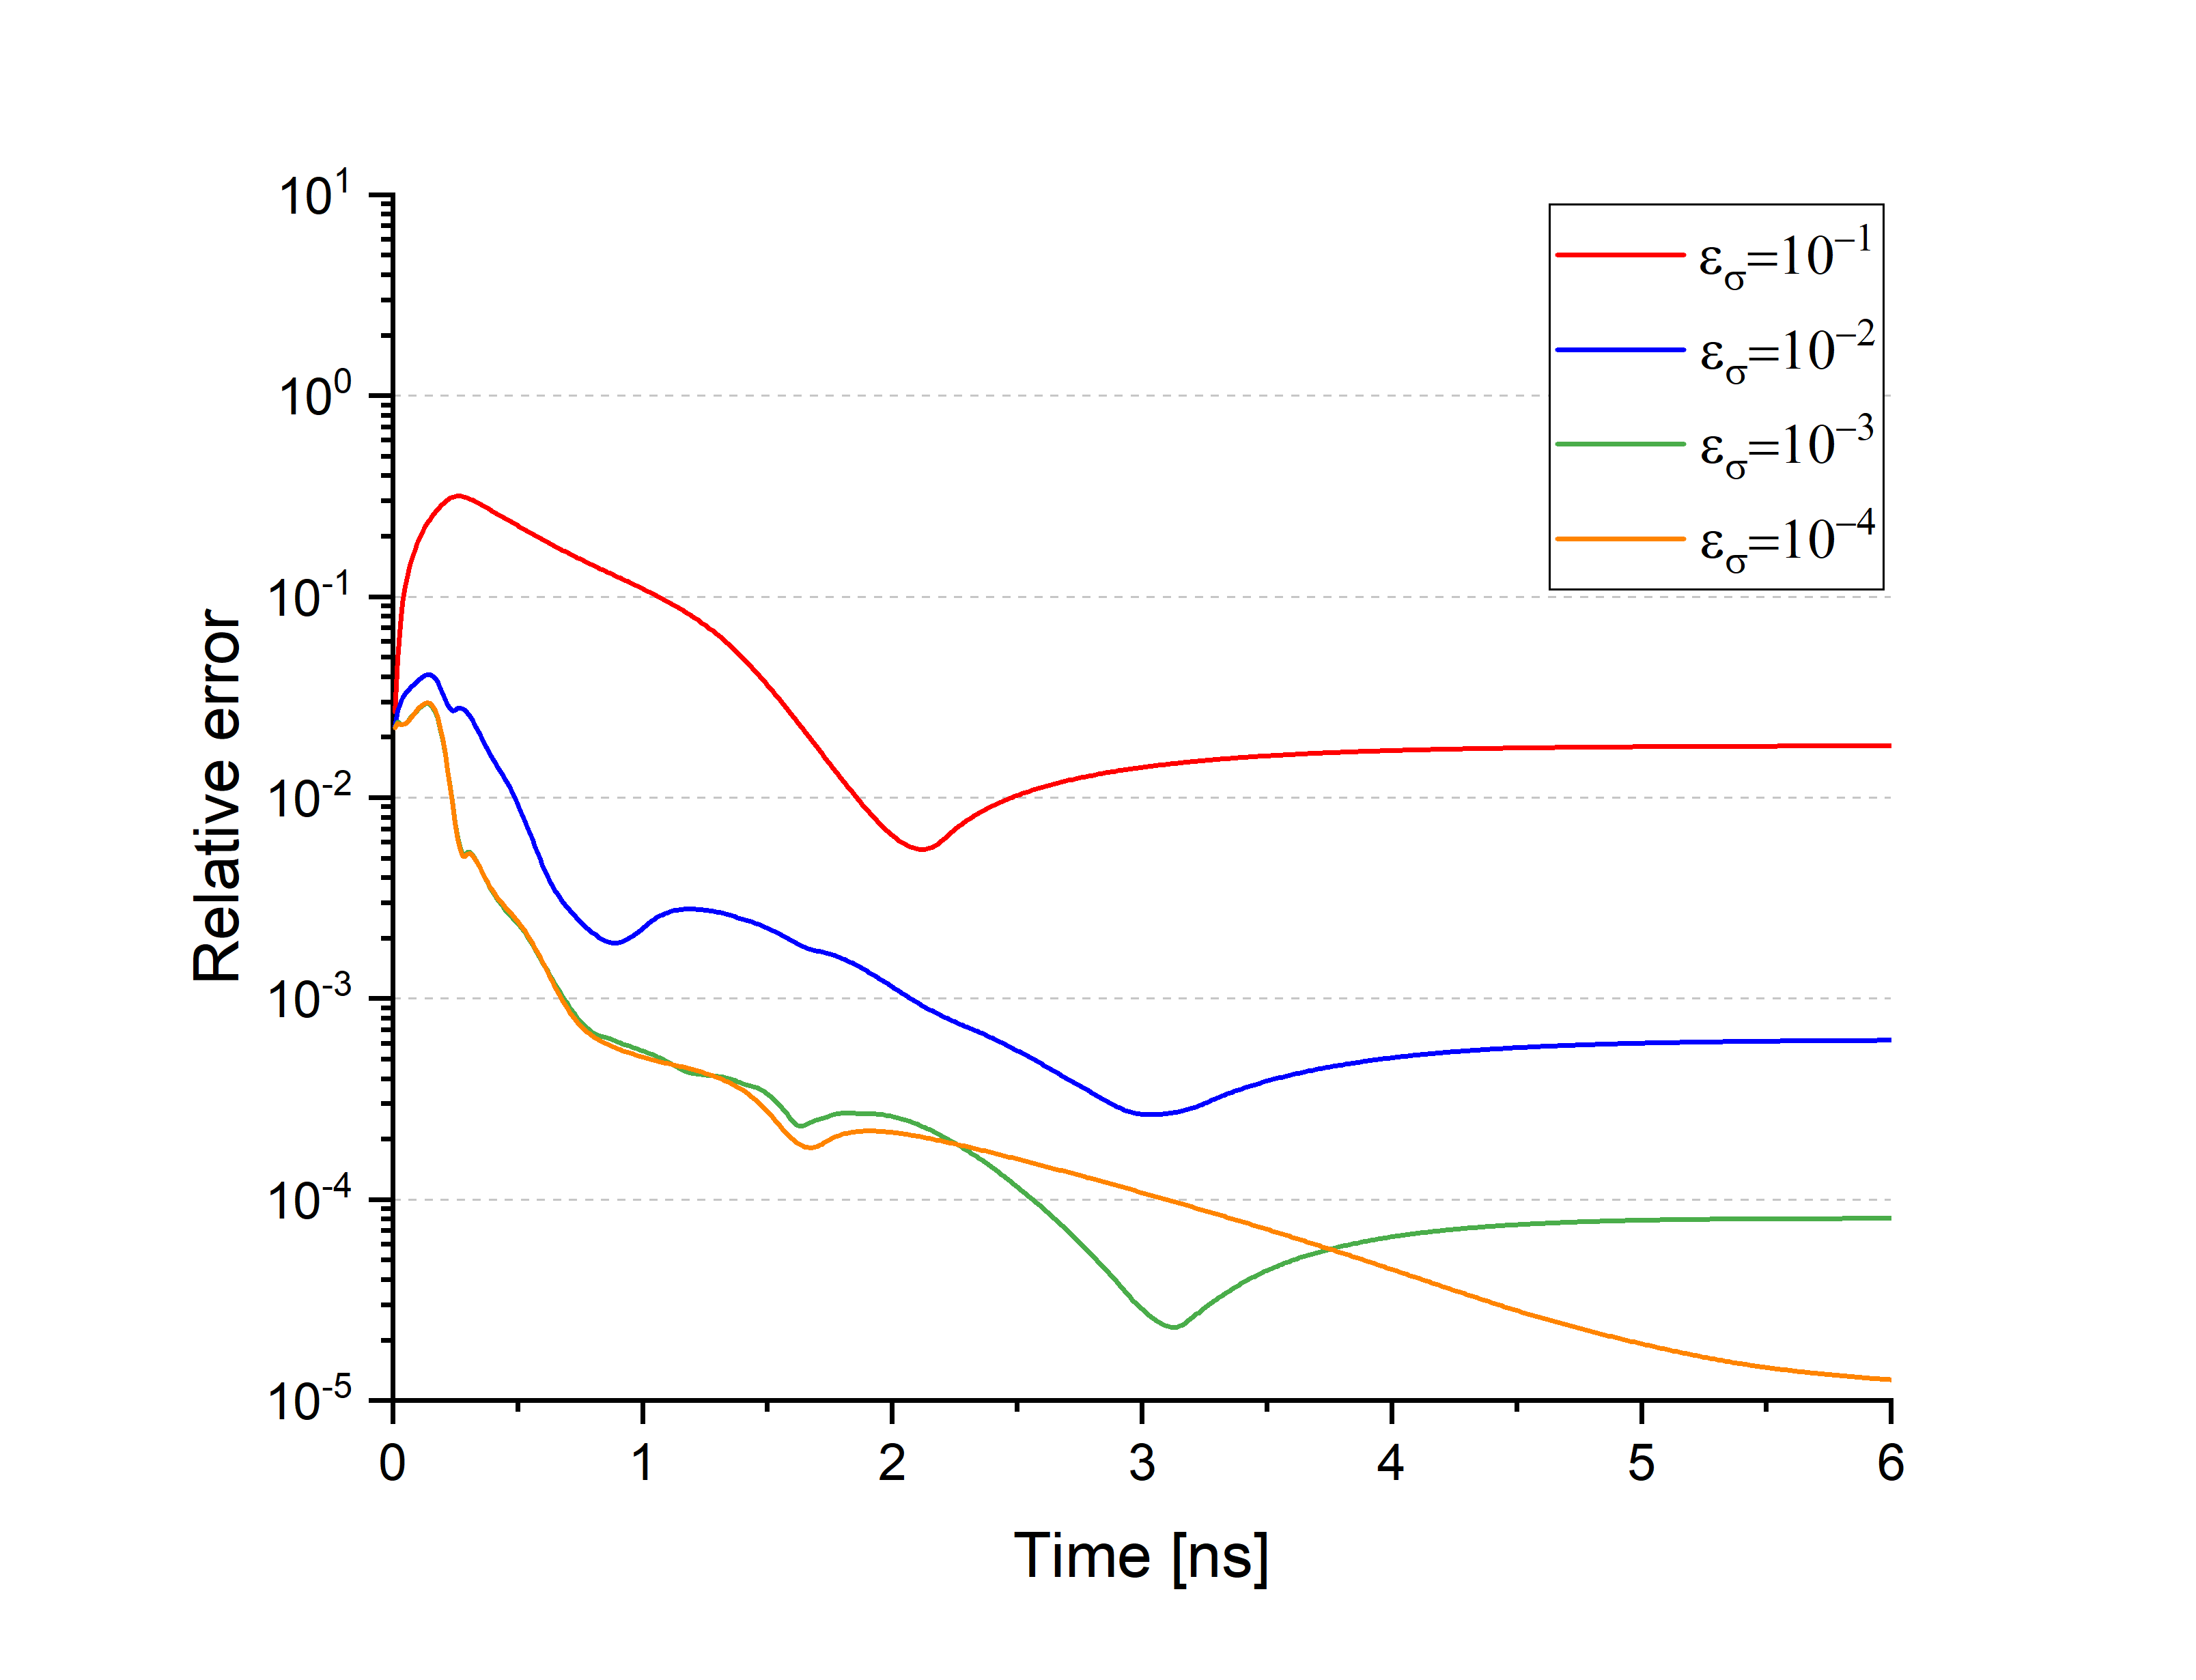
\includegraphics[width=0.5\textwidth]{MG_bc960-t001_qdf1000-920-t002_Tavg_mlqd.png}}
		\subfloat[Energy density relative error \label{subfig:MG_bc960-t001_qdf1000-920-t002_Eavg_mlqd}]{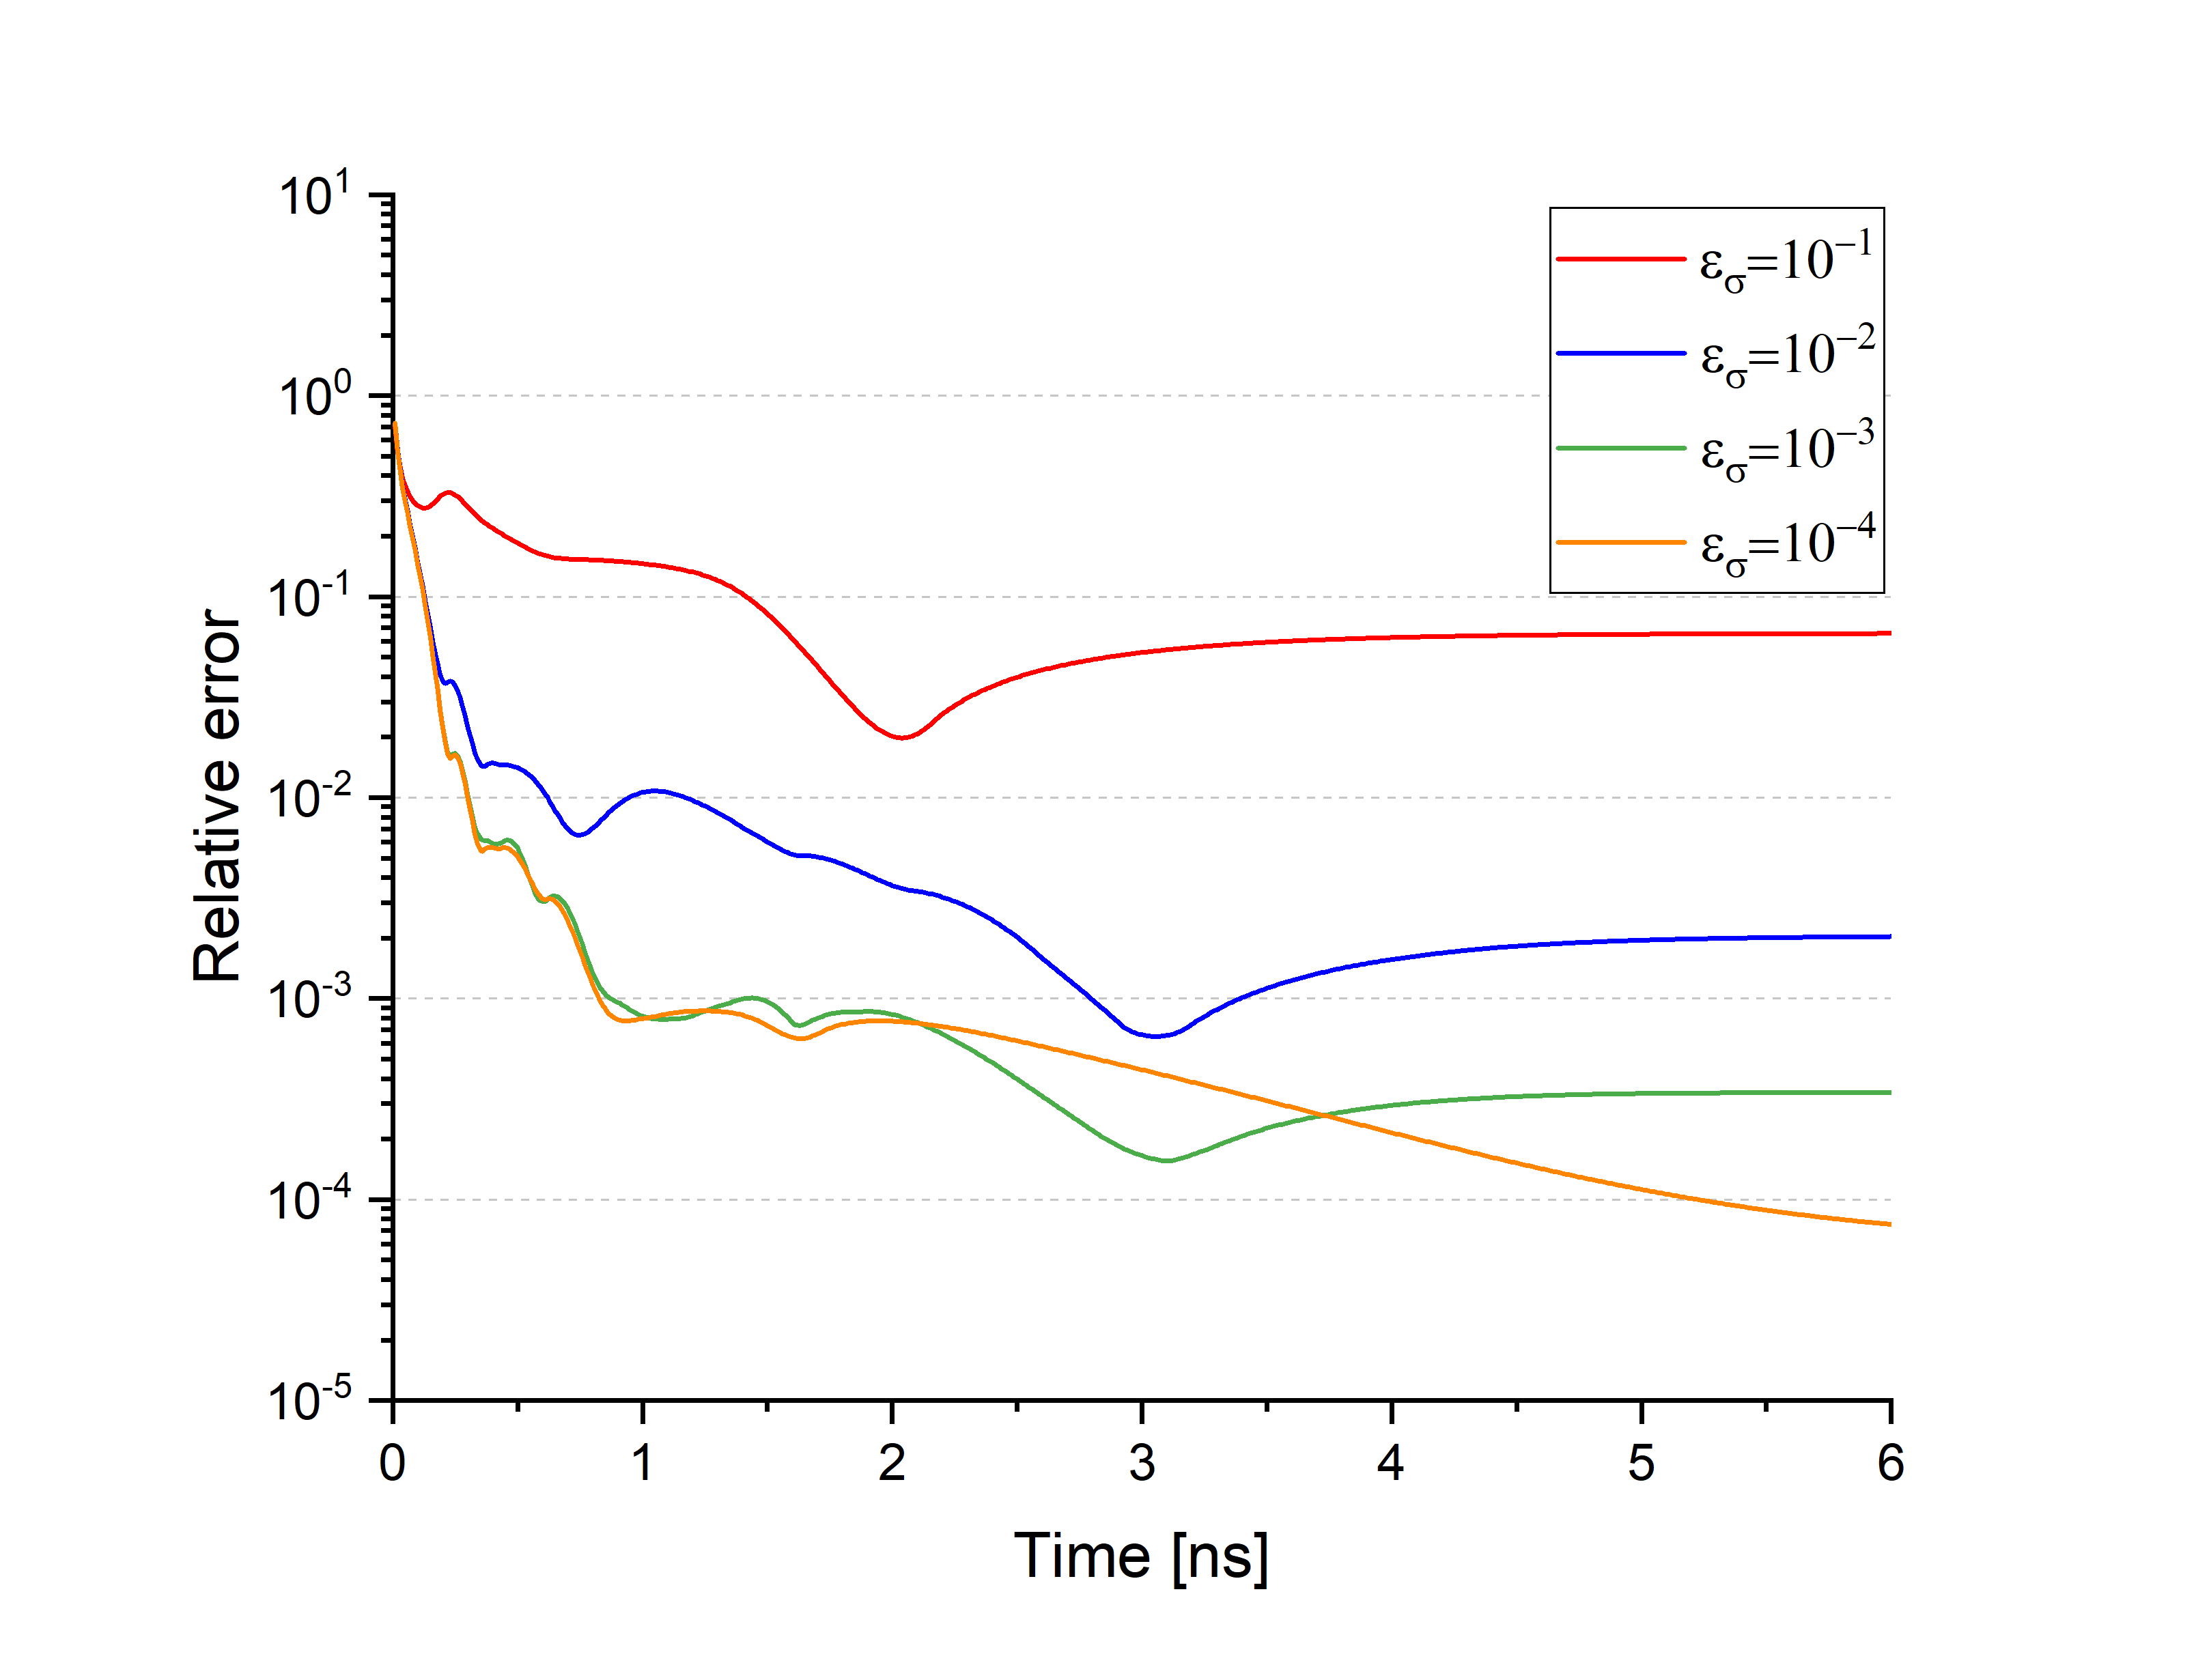
\includegraphics[width=0.5\textwidth]{MG_bc960-t001_qdf1000-920-t002_Eavg_mlqd.png}}
		\caption{\label{fig:errors_bc_T=960_t001}
			Relative error in the $L_1$-norm of the MLQD-POD solutions computed with $T_{in}~=~0.96$~KeV and $\Delta t\! =\! 1 \! \times \! 10^{-2}$~ns using base cases with $T_{in}^{\pr{1}}=1$ KeV  and $T_{in}^{\pr{2}}=0.92$ KeV and $\Delta t\! =\! 2 \! \times\!  10^{-2}$.}
	\end{figure}


\chapter{A ROM Based on the Grey LOQD Equations and Proper Orthogonal Decomposition of QD Factors and Energy Density Spectrum}
\label{chap-four}

\newcommand{\amodkapebin}{\kapebin^{\tau*}}
\newcommand{\amodkaprbirn}{\kaprbirn^{\tau*}}
\newcommand{\amodkapgirn}{\kapgirn^{\tau*}}
\newcommand{\amodkapgirrn}{\kapgirrn^{\tau*}}

\newcommand{\aetailnp}{\eta_{i-\frac{1}{2},n}^{+*}}
\newcommand{\aetailnm}{\eta_{i-\frac{1}{2},n}^{-*}}
\newcommand{\aetairnp}{\eta_{i+\frac{1}{2},n}^{+*}}
\newcommand{\aetairnm}{\eta_{i+\frac{1}{2},n}^{-*}}

This chapter develops a ROM for solving TRT problems based on the effective grey problem described in Sec. \ref{eff_gr_prb}. The POD (Sec. \ref{sec:pod}) is used to approximate the group QD factors and the solution of the multigroup LOQD system. Section \ref{sec:pod-qd} formulates the ROM, henceforth referred to as the GLOQD-POD ROM. Sections \ref{reduced_eg} and \ref{bb_cor} analyze the POD of the group radiation energy densities and formulate a method of correcting those approximate radiation energy densities. Section \ref{sec:gloqd-pod_res} describes the numerical results of this ROM.

%=================================================================================
% POD-BASED REPRESENTATION  OF SPECTRUM
%=================================================================================
\section{Formulation of the GLOQD-POD ROM} \label{sec:pod-gqd} 
	We apply the POD methodology on the discrete set of group energy densities $E_g(x,t)$. The discrete group energy densities are defined on grids of energy, space and time, and the POD is applied to each energy group separately to obtain approximations over space and time \cite{dya-jcp-2019}. The same procedure as applied to the group QD factors (Ch. \ref{chap-three}) is followed by forming $N_g$ group-wise matrices $\bA^{E}_g \in \real^{\chi,\tau}$ where each matrix holds the set of group $g$ energy densities. $\chi$ and $\tau$ are the number of discrete spatial and temporal nodes respectively. Each column in $\bA^E_g$ contains the spatial vector of the group energy densities at a separate instant of time, ordered chronologically. The SVD  is applied to each $\bA^E_g$ to cast in the form of \eqn{svd_form}, $\bA^E_g = \bU_g\bSig_g\bV_g^T$ where $\bU_g \in \real^{\chi,k}$, $\bSig_g \in \real^{k,k}$, $\bV_g \in \real^{\tau,k}$, and $k = \min\pr{\chi,\tau}$. The reduced rank approximation of each group energy density matrix is given as $\bA^{E*}_g  = \bU^*_g\bSig^*_g\pr{\bV^{*}_g}^T $ where $\bU^*_g \in \real^{\chi,r_g}$, $\bSig^*_g \in \real^{r_g,r_g}$, $\bV^{*}_g \in \real^{\tau,r_g}$. $r_g$ is the reduced rank determined by $\varepsilon_\sigma$ (Eq. \ref{cutoff_eps}), and the $\gamma_n$ of the singular values used is calculated as $\gamma_{r_g}$ (Eq. \ref{worth_gam}).
	
	\ind Given approximate QD factors $f_g^*$ and radiation energy densities $E_g^*$ calculated with a low-rank POD, a set of corresponding group radiation fluxes at each instant of time $\bFg^*\pr{x,t}$ can be calculated with the multigroup MLOQD-POD system \eqref{mqd_sys}. This defines group radiation fluxes according to the group first moment QD equation (Eq. \ref{mqd_2}) and the reduced rank group radiation energy densities. The quantities required for the effective grey problem are calculated with the approximate multigroup solution and group QD factors. The approximate grey QD factors are calculated as
	\begin{align}
		\bar{f}^*\pr{x,t} = \frac{ \sum_{g=1}^{N_g}\fg^*\pr{x,t}\eg^*\pr{x,t} }{ \sum_{g=1}^{N_g}\eg^*\pr{x,t} },
	\end{align}
	
	where $\fg^*$ and $\eg^*$ are the approximate group QD factors and radiation energy densities obtained from the low-rank POD, namely, $\bA^{f*}_g$ and $\bA^{E*}_g$. Similarly we define two approximate grey opacities \eqref{grey_opacities}
	\begin{gather}
		\kapeb^*\pr{T} = \frac{ \sum_{g=1}^{N_g}\kapg\pr{T}\eg^*\pr{x,t} }{ \sum_{g=1}^{N_g}\eg^*\pr{x,t} }, \\[5pt]
		\kaprb^*\pr{T} = \frac{ \sum_{g=1}^{N_g}\kapg\pr{T}\abs{\bFg^*\pr{x,t}} }{ \sum_{g=1}^{N_g}\abs{\bFg^*\pr{x,t}} },
	\end{gather}
	
	and the compensation factor \eqref{eta_comp} is calculated as
	\begin{equation}
		\eta^*\pr{x,t} = \frac{ \sum_{g=1}^{N_g}\brk{\pr{\kapg\pr{T} - \kaprb^*\pr{T}}\bFg^*\pr{x,t}} }{ \sum_{g=1}^{N_g}\eg^*\pr{x,t} }.
	\end{equation}
	
	The GLOQD-POD ROM is characterized by the resulting GLOQD and MEB equations using approximate quantities
	\begin{subequations}
		\begin{gather}
			\dt{\eb\pr{x,t}} + \grad\cdot\bFb\pr{x,t} + c\kapeb^*\pr{T}\eb\pr{x,t} = c\kapbb^*\pr{T}\ar T^4 \label{glqd_pod_zero} \\
			\frac{1}{c}\dt{\bFb\pr{x,t}} + c\grad\cdot\pr{\fb^*\pr{x,t}\eb\pr{x,t}} + \kaprb^*\pr{T}\bFb\pr{x,t} + \eta^*\pr{x,t}\eb\pr{x,t}= 0 \label{glqd_pod_first} \\
			\dt{\varepsilon\pr{T}} = c\kapeb^*\pr{T}\eb\pr{x,t} - c\kapbb^*\pr{T}\ar T^4. \label{EB_gpod}
		\end{gather}
		\label{glqd_pod_eqs}
	\end{subequations}

	\iffalse
	In discrete space the GLOQD-POD ROM is
	\begin{subequations}
		\begin{gather}
			\Fbirn - \Fbiln + c\delxi\amodkapebin\pr{T}\ebin = c\kapbbin^*\pr{T}\ar T^4_{i,n} + \frac{\ebinl}{\deltn}
		\end{gather}
		\vspace*{-1.2cm}
		\begin{multline}
			c\pr{\fbirrn^*\ebirrn - \fbin^*\ebin} + \delxir\amodkaprbirn\pr{T}\Fbirn \\+ \pr{\aetairnp\ebirrn - \aetairnm\ebin} = \delxir\frac{\Fbirnl}{c\deltn}
		\end{multline}
		\vspace*{-.9cm}
		\begin{gather}
			\frac{\varepsilon_{i,n}\pr{T} - \varepsilon_{i,n-1}\pr{T}}{\delt_n} = c\kapebin^*\ebin - c\ar\kapbbin^*\tin^4\\
			i = 1,\dots,I, \ n = 1,\dots,N_n \nn
		\end{gather}
	\end{subequations}
	\fi
	
	
	\iffalse
	 as the elements of the $n^{\text{th}}$ column of the low-rank SVD of $\bA_g^f$ and $\bA_g^E$ respectively
	\begin{equation}
		\fgin^* = \Big(a^{f*}_{i,n}\Big)_g, \ \
		\egin^* = \Big(a^{E*}_{i,n}\Big)_g,
	\end{equation}
	
	with $\pr{a^{f*}_{i,n}}_g$ and $\pr{a^{E*}_{i,n}}_g$ as the $\pr{i,n}$ element of the matrices $\bA_g^{f*}$ and $\bA_g^{E*}$.
	\fi
	 
	
	\iffalse
	The discrete grey opacities are
	\begin{subequations}
		\begin{gather}
			\kapebin^*\pr{T} = \frac{ \sum_{g=1}^{N_g}\kapgin\pr{T}\egin^* }{ \sum_{g=1}^{N_g}\egin^* } \\[5pt]
			\kapbbin\pr{T} = \frac{ \sum_{g=1}^{N_g}\kapgin\pr{T}\Bgin\pr{T} }{ \sum_{g=1}^{N_g}\Bgin\pr{T} } \\[5pt]
			\kaprbirn^*\pr{T} = \frac{ \sum_{g=1}^{N_g}\kapgirn\pr{T}\abs{\Fgirn^*} }{ \sum_{g=1}^{N_g}\abs{\Fgirn^*} },
		\end{gather}
	\end{subequations}
	
	and the modified opacities are
	\begin{subequations}
	\begin{gather}
		\amodkapebin\pr{T} = \kapebin^*\pr{T} + \frac{1}{c\deltn}, \\
		\amodkaprbirn\pr{T} = \kaprbirn^*\pr{T} + \frac{1}{c\deltn}.
	\end{gather}
	\end{subequations}
	
	The discrete compensation term is
	\begin{subequations}
		\begin{align}
			&\etairn^* = \sum_{g=1}^{N_g} \brk{\pr{\kapgirn - \kaprbirn^*}\Fgirn^*}\\
			&\aetairnp = \left\{ \begin{array}{ll}
						\frac{\etairn^*}{\sum_{g=1}^{N_g} \egirrn^*} & \etairn^*>0\\
						0 & \etairn^*<0
					\end{array} \right.\\
			&\aetairnm = \left\{ \begin{array}{ll}
						0 & \etairn^*>0\\
						\frac{-\etairn^*}{\sum_{g=1}^{N_g} \egin^*} & \etairn^*<0
					\end{array} \right.
		\end{align}
	\end{subequations}
	\fi
	
	In discrete space this ROM is given by the GLOQD Eqs. \eqref{gqd_sys_disc} and MEB Eq. \eqref{ebdisc2} with the POD quantities described in this section. The group cell average QD factors and radiation energy densities at each instant of time $\pr{n}$ are defined as described for $\fgin^*$ in Sec. \ref{sec:pod-qd}. The radiation flux $\Fgirn^*$ is calculated with the MLOQD-POD system \eqref{mlqd_pod_eqs} given $\fgin^*$ and $\egin^*$. Note that the derived ROM does not solve the RT or MLOQD equations except to update the group radiation fluxes. Algorithm \ref{alg:glqd_rom_alg} shows the iterative scheme for the GLOQD-POD ROM for TRT problems.
	
	\begin{algorithm}[ht!]
		\SetAlgoLined
		\While{$t^n<t^{\text{end}}$}{
			$n=n+1$\\
			$T^{\pr{0}} = T^{n-1}$\\
			$\bfg^* \leftarrow \bA^{f*}_g$, \ \ $\eg^* \leftarrow \bA^{E*}_g$\\
			%Calculate $\bFg$ from MLOQD-POD Eqs. \eqref{mlqd_pod_eqs}\\
			\While{$\norm{T^{\ell}-T^{\ell-1}} > \tilde{\epsilon}_1\norm{T^{\ell}} + \tilde{\epsilon}_2, \ \ \norm{\eb^{\ell}-\eb^{\ell-1}} > \tilde{\epsilon}_1\norm{\eb^{\ell}} + \tilde{\epsilon}_2 $}{
				$\ell=\ell+1$
				Update opacities $\kapg\pr{T^{\ell}}$\\
				Update group radiation fluxes $\bFg^*$ with MLOQD-POD Eqs. \eqref{mlqd_pod_eqs}\\
				Compute grey quantities $\kapeb^{*,\ell}$, $\kapbb^{\ell}$, $\kaprb^{*,\ell}$, $\bfb^{*,\ell}$, $\etab^{*,\ell}$\\
				Solve coupled GLOQD-POD and MEB Eqs. \eqref{glqd_pod_eqs} for $\eb^{\ell}$, $\bFb^{\ell}$, $T^{\ell}$
			}
			$T^n \leftarrow T^\ell$
		}
		\caption{Nonlinear QD Iterative Scheme for the GLOQD-POD ROM using reduced rank databases of group QD factors $\bA^{f*}_g$ and group radiation energy densities $\bA^{E*}_g$ \label{alg:glqd_rom_alg}}
	\end{algorithm}
	
%=================================================================================
% Numerical Results
%=================================================================================
%\section{Test Problem Formulation} \label{sec:gpod_test} 
%	In this section we present computational results for the same 1D F-C test as described for section \ref{sec:mpod_test}. Given the same test conditions, the analysis for the reduced rank QD factors is equivalent to that shown in section \ref{sec:reduced_qdf}.

\section{Low-Rank Approximation of Group Energy Densities} \label{reduced_eg}
	%In this section computational results are presented for the same 1D F-C test as described for Sec. \ref{sec:mpod_test}. Given the same test conditions, the analysis for the reduced rank group QD factors is equivalent to that shown in section \ref{sec:reduced_qdf}.
	
	Analysis of reduced rank forms of the group QD factors is given in Ch. \ref{chap-three}. Fig. \ref{fig:Eg_sval_summary} displays the normalized magnitudes and $1-\gamma_n$ of the singular values of $\bA^E_g$ for each energy group. Since the test problem has 60 spatial cells the vector of cell-average group radiation energy densities in space has 62 values including 2 boundary values. When $\varepsilon_\sigma=10^{-12}$, the full-rank SVD is used. The low energy groups $g=\pr{1,2,3,4}$ require the highest ranks for the shown values of $\varepsilon_\sigma$ and the middle groups require the lowest ranks. The singular values normalized to the largest singular value for all energy groups are shown in Fig. \ref{subfig:EG_Svals_grey}, where each energy group has a horizontal plateau of values that starts at roughly $r=30$. These plateaus decrease in magnitude as $g$ is increased. Note that there is a large gap between the observed plateaus of groups 1,2,3 and the latter energy groups. The same behavior is shown for the values of $1-\gamma_n$ for each energy group in Fig. \ref{subfig:inv_worths_Eg_grey}. The higher energy groups reach numerically zero ($10^{-16}$) for $1-\gamma_n$ at roughly the same point where the singular value plateau occurs. The large gap between low energy groups and middle to high energy groups implies low energy groups to be the most difficult to approximate with low rank forms. Table \ref{tab:gqd_sigtab} displays the rank of approximation $(r_g)$ involved per energy group at different values of  $\varepsilon_\sigma$.
	
	%=================================================================================
	% SINGULAR VALUE FIGS
	\begin{figure}[ht!]
		\centering
		\subfloat[Normalized singular values of $\bA^E_g$ (group radiation energy density database matrices) \label{subfig:EG_Svals_grey}]{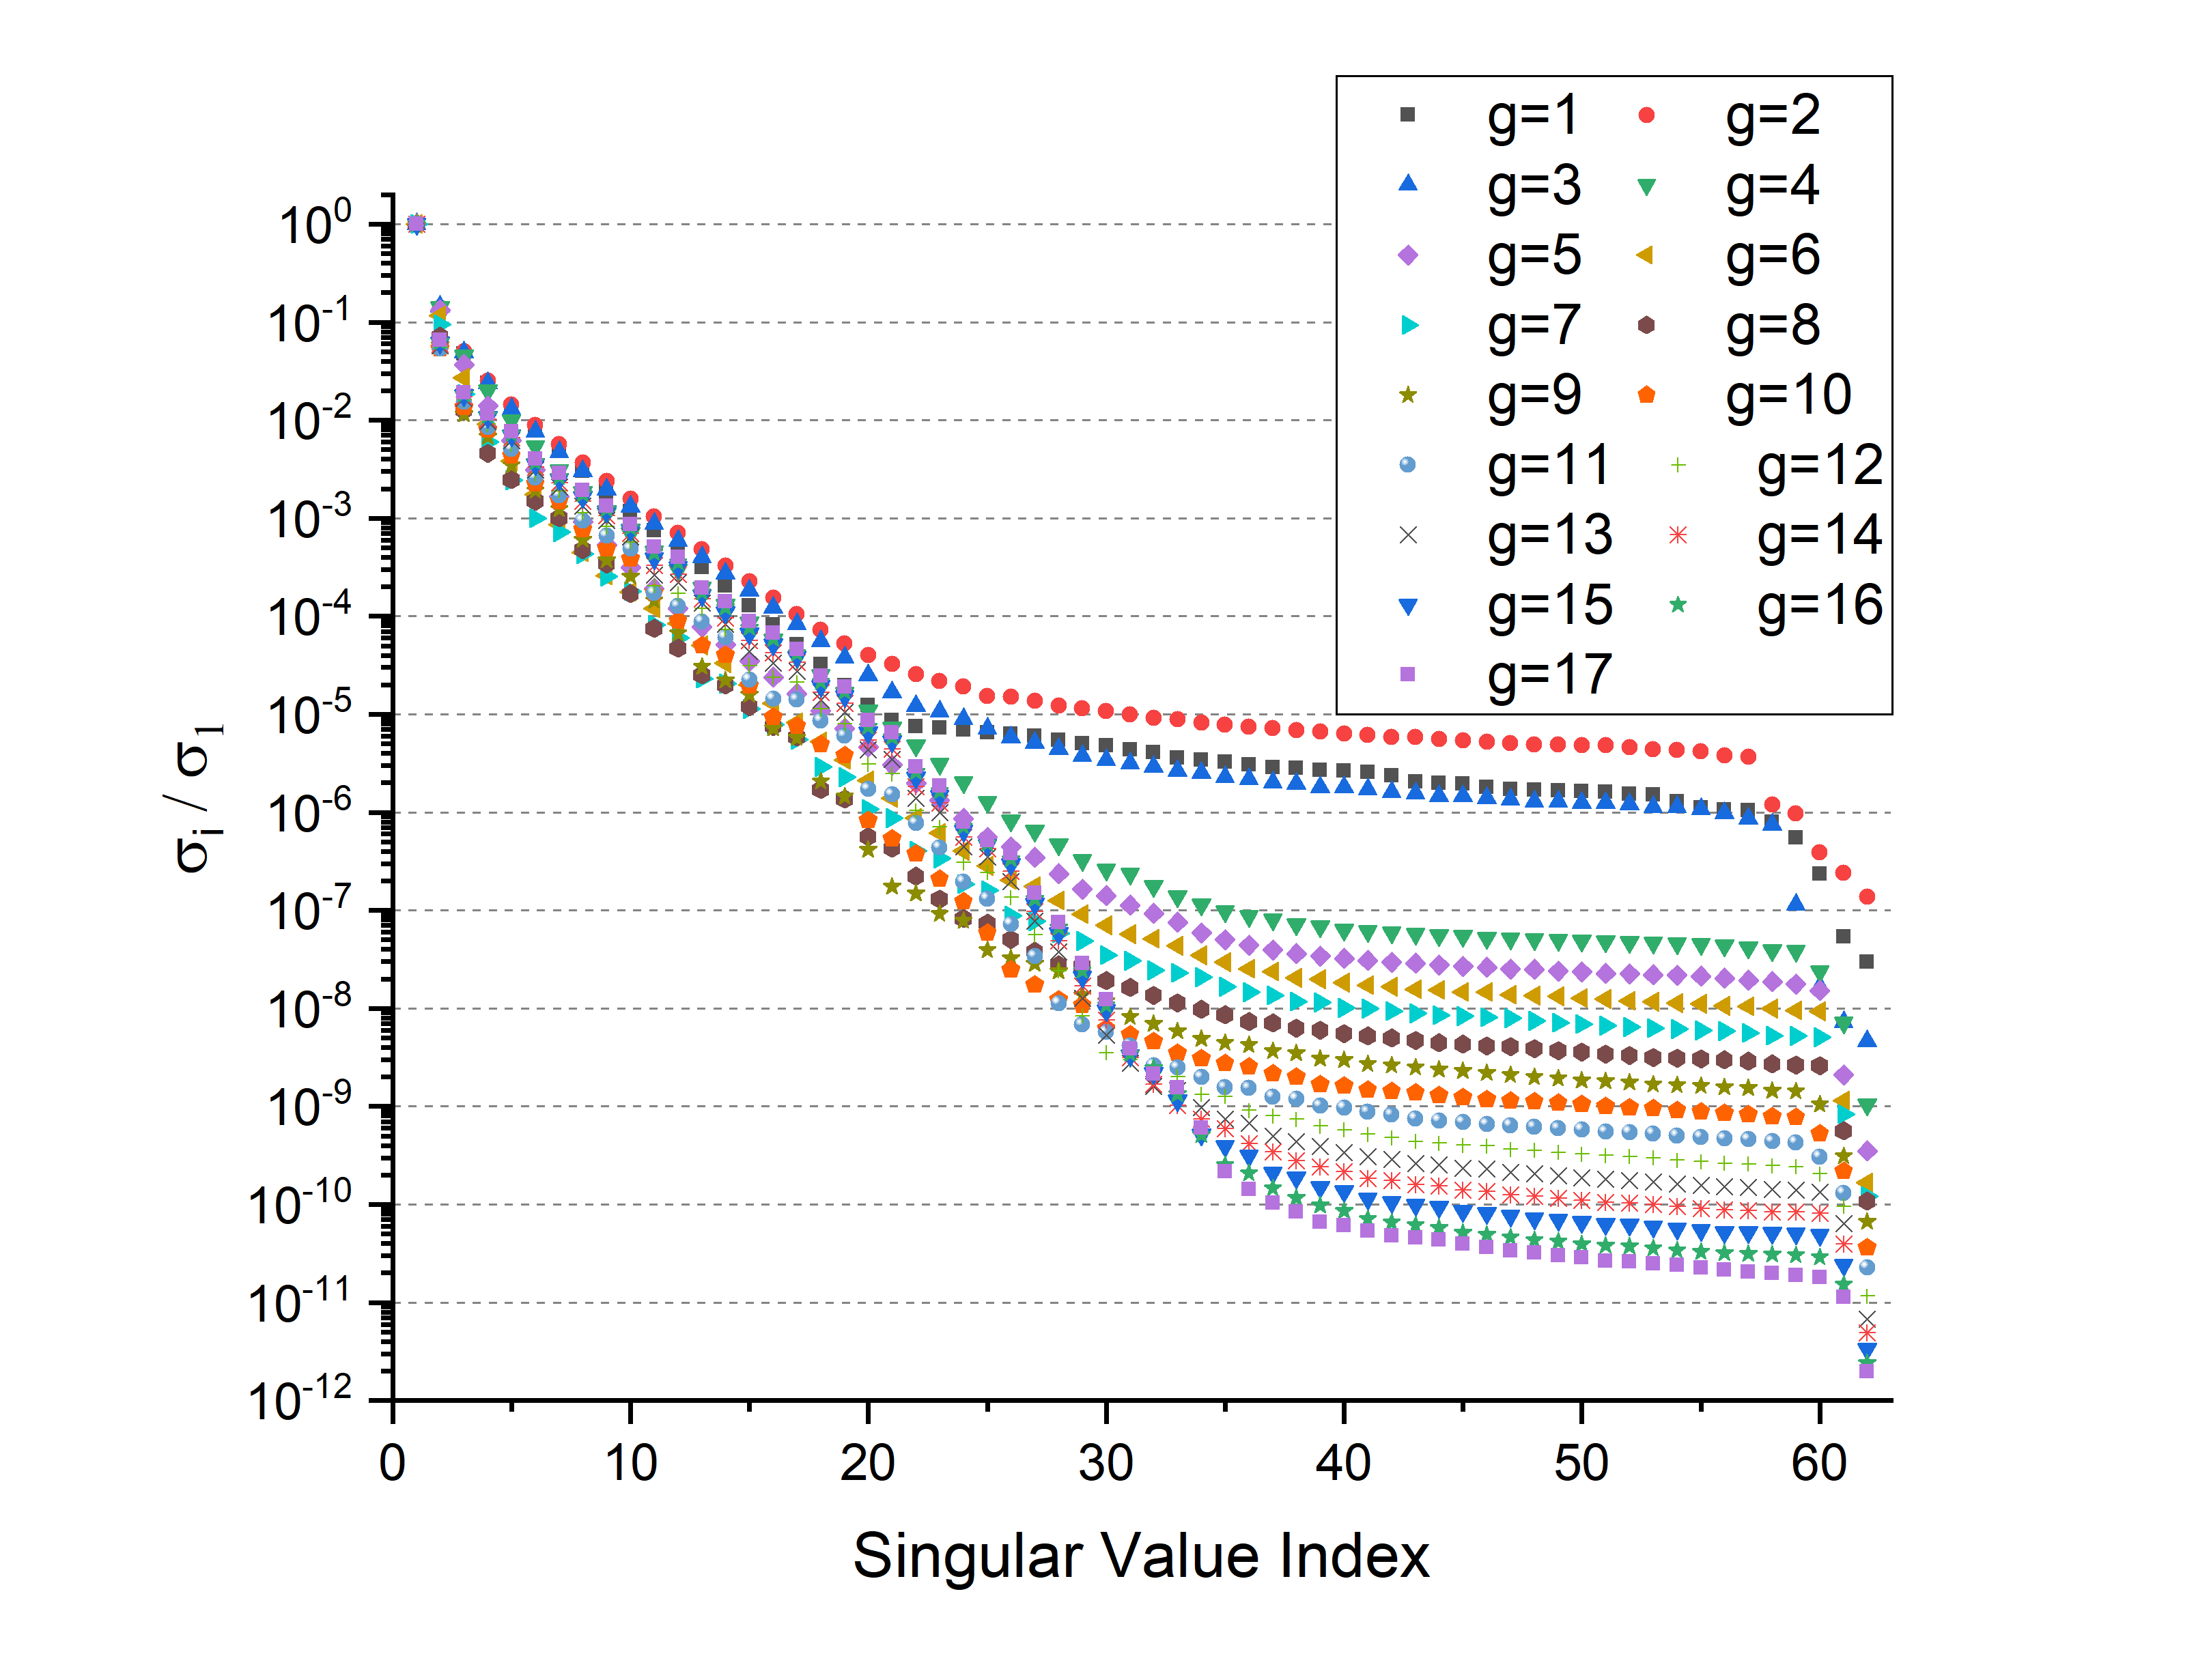
\includegraphics[width=0.5\textwidth]{Eg_normalized_svals.png}} \hspace*{.5cm}
		\subfloat[$1-\gamma_n$ for $\bA^E_g$ (group radiation energy density database matrices) \label{subfig:inv_worths_Eg_grey}]{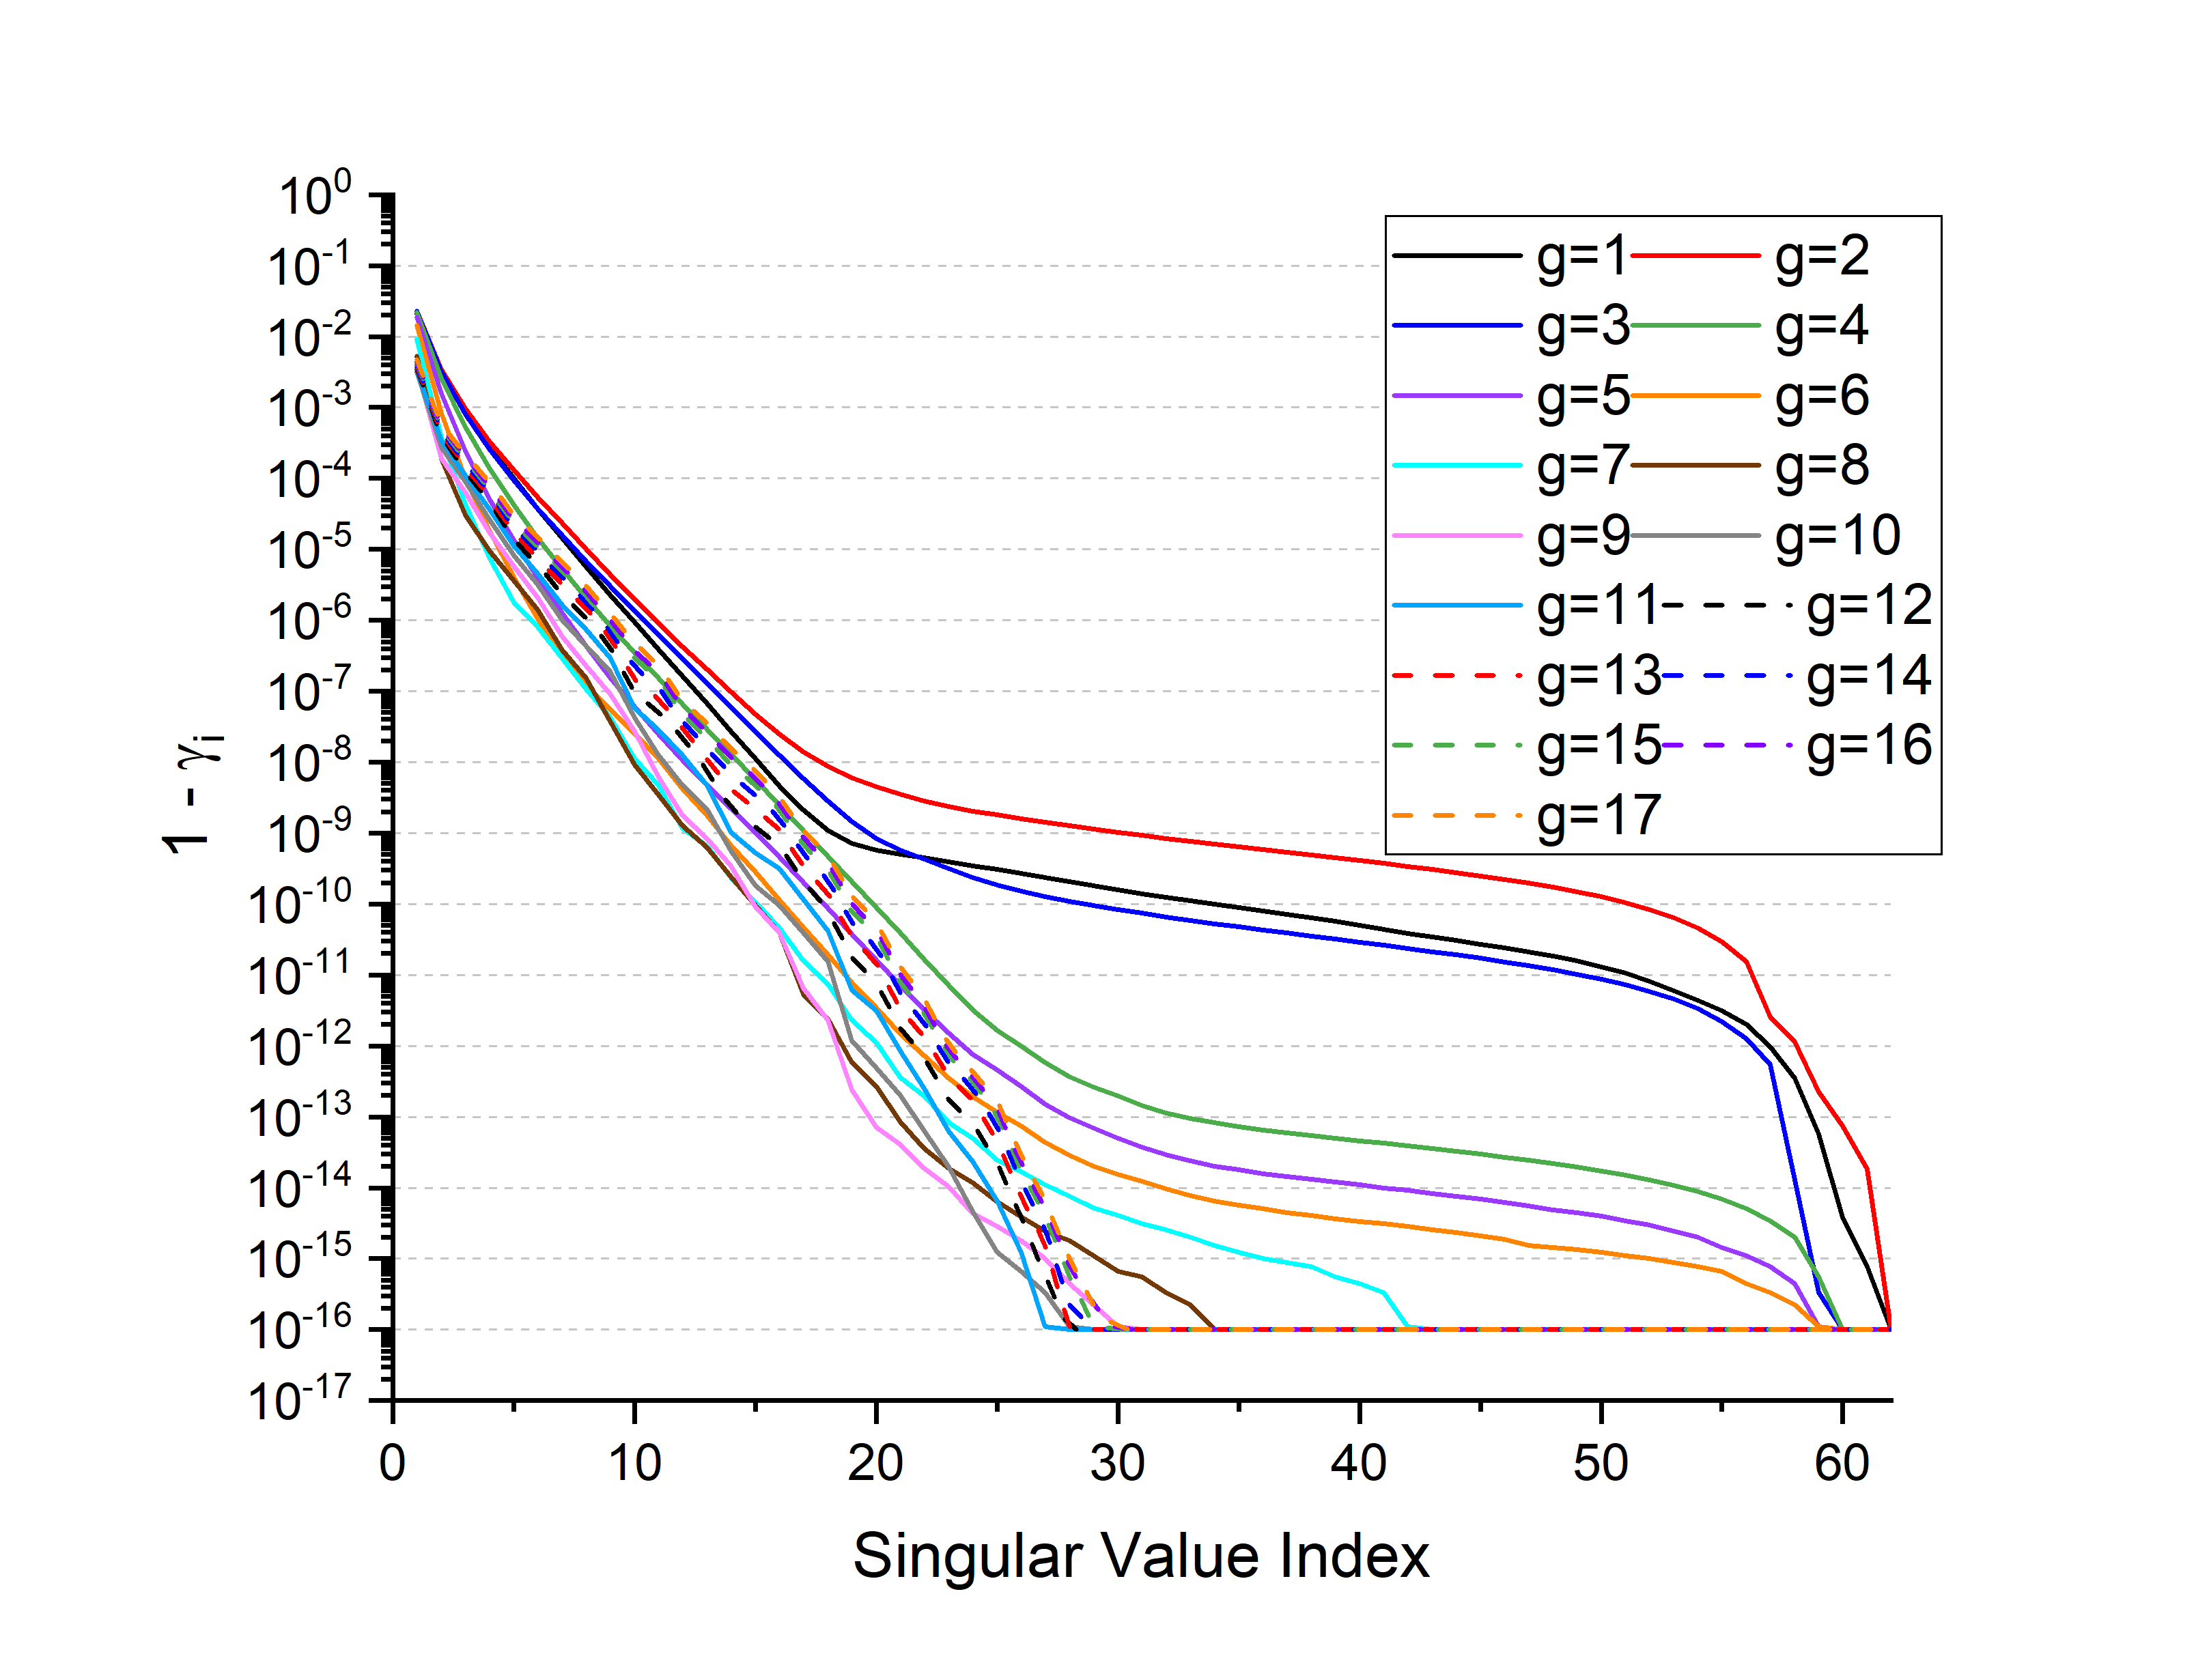
\includegraphics[width=0.5\textwidth]{inv_worths_Eg_grey.png}}
		\caption{\label{fig:Eg_sval_summary}
			Group radiation energy density normalized singular values and $1-\gamma_n$}
	\end{figure}
	
	%=================================================================================
	% SINGULAR VALUE TABLE
	\begin{table}[ht!]
		\caption{	\label{tab:gqd_sigtab} The rank of approximation $(r_g)$ of $E_g$ in each energy group for decreasing values of $\varepsilon_\sigma$}
		\begin{tabular}{|c||c|c|c|c|c|c|c|c|c|c|c|c|c|c|c|c|c|}	
			\hline
			$\varepsilon_\sigma \backslash  \ g$ & 1 & 2 & 3 & 4 & 5 & 6 & 7 & 8 & 9 & 10 & 11 & 12 & 13 & 14 & 15 & 16 & 17 \\
			\hline
			\hline
			$10^{-1}$ & 2  &  2 & 2  & 2  & 2  & 2  &  1 & 1 &  1 &   1 & 1 &  1 &  1 & 1 &  1 &  1 & 1 \\ \hline
			$10^{-2}$ & 5 & 5 & 5 & 4 & 4 & 3 & 3 & 3 & 3 & 3 & 3 & 3 & 3 & 4 & 4 & 4 & 4\\ \hline
			$10^{-3}$ & 10 & 11 & 10 & 9 & 7 & 6 & 5 & 7 & 7 & 7 & 7 & 8 & 8 & 9 & 9 & 9 & 9\\ \hline
			$10^{-4}$ & 15 & 17 & 16 & 14 & 12 & 11 & 10 & 10 & 11 & 11 & 12 & 13 & 13 & 13 & 14 & 14 & 14\\ \hline
			$10^{-12}$ & 62 & 62 & 62 & 62 & 62 & 62 & 62 & 62 & 62 & 62 & 62 & 62 & 62 & 62 & 62 & 62 & 62\\ \hline
		\end{tabular}
	\end{table}

	\ind Next the reduced rank forms of the group radiation energy densities are investigated. The same select energy groups $g=\pr{2,3,8}$ as considered for the group QD factors in Ch. \ref{chap-three} are used. Once again, groups 2 and 3 are representative of the most inaccurate energy groups when approximated with low rank and group 8 acts as a representative for the rest of the group radiation energy densities. Figs. \ref{fig:Eg_g2_recomps}, \ref{fig:Eg_g3_recomps} and \ref{fig:Eg_g8_recomps} show the reduced rank group radiation energy densities for groups 2, 3 and 8 respectively. Each of these figures displays the group radiation energy densities reduced to 6 different ranks $r=\pr{1,2,5,10,15,20}$. For all plots shown when $r=20$, the structure of the group radiation energy densities has converged to the reference solution to the resolution of the plot. Groups 2 and 3 display very similar structures for all shown instants of time, which differs from group 8. 
	
	\ind The group radiation energy densities for groups 2 and 3 have converged to the resolution of the plot by the $r=15$. Group 8 shows convergence to the resolution of the plot once $r=10$. The reduced rank forms for all groups are the most inaccurate when approximating energy densities of very small magnitudes. Groups 2 and 3 most easily depict this effect, with visibly oscillatory behavior at early instants of time when the energy densities have a sharp gradient near the end of the radiation wave. This is similar to the behavior of approximate group QD factors in groups with sharp gradients or discontinuities as shown in Ch. \ref{chap-three}. Some of the reduced rank forms of the group radiation energy densities become nonphysically negative due to this oscillatory structure. Most evident in Figs. \ref{subfig:Eg_g2_cut5_grey} and \ref{subfig:Eg_g3_cut5_grey}, the energy densities become largely negative for part of the spatial domain to the right of the radiation wave. This effect persists beyond the resolution of the plots and the magnitude of these negative values is simply decreased as higher rank approximations are used. 
	
	\ind The accuracy of the reduced rank form of the group energy densities is also constrained by numeric limitations. During early times some of the low energy groups have energy densities near the right boundary that are much less than $10^{-15}$ $\text{tera-erg (Terg)}$ where $\text{Terg} = 10^{12} \ \text{erg}$ are computational units. The use of such computational units is a standard and common approach in physics (and engineering) to deal with orders of magnitude of values. The rest of the energy groups display energy densities on the order of $10^{-6} \ \text{to} \ 10^{-8} \ \text{Terg}$ near the right boundary. This is expected as for early times the radiation incoming from the left boundary has not been able to propagate far into the slab of material and thus only low energy background radiation is present near the right boundary. Given that the left boundary energy density for all groups is on the order of $10 \ \text{Terg}$ or greater, the POD inaccurately recreates values of less than $10^{-16} \ \text{ergs}^*$ due to a loss of significance caused by finite-precision arithmetics. For the same reason, energy densities with values greater than $10^{-15} \ \text{Tergs}$ may only have a few digits of accuracy if near $10^{-1} \ \text{Terg}$. Thus the full rank POD is unable to recreate the exact matrix of radiation energy densities that was decomposed.

	%=================================================================================
	% Eg G2 RECOMP
	\begin{figure}[ht!]
		\centering
		\subfloat[r = 1 \label{subfig:Eg_g2_cut1_grey}]{\includegraphics[width=0.5\textwidth]{Eg_g2_cut1_grey.png}}
		\subfloat[r = 2 \label{subfig:Eg_g2_cut2_grey}]{\includegraphics[width=0.5\textwidth]{Eg_g2_cut2_grey.png}}\\
		\subfloat[r = 5 \label{subfig:Eg_g2_cut5_grey}]{\includegraphics[width=0.5\textwidth]{Eg_g2_cut5_grey.png}}
		\subfloat[r = 10 \label{subfig:Eg_g2_cut10_grey}]{\includegraphics[width=0.5\textwidth]{Eg_g2_cut10_grey.png}}\\
		\subfloat[r = 15 \label{subfig:Eg_g2_cut15_grey}]{\includegraphics[width=0.5\textwidth]{Eg_g2_cut15_grey.png}}
		\subfloat[r = 20 \label{subfig:Eg_g2_cut20_grey}]{\includegraphics[width=0.5\textwidth]{Eg_g2_cut20_grey.png}}
		\caption{\label{fig:Eg_g2_recomps}
			Low-rank approximations of the group radiation energy density ($E_g^*$) based on the POD for $g=2$ for select time steps}
	\end{figure}
	
	%=================================================================================
	% Eg G3 RECOMP
	\begin{figure}[ht!]
		\centering
		\subfloat[r = 1 \label{subfig:Eg_g3_cut1_grey}]{\includegraphics[width=0.5\textwidth]{Eg_g3_cut1_grey.png}}
		\subfloat[r = 2 \label{subfig:Eg_g3_cut2_grey}]{\includegraphics[width=0.5\textwidth]{Eg_g3_cut2_grey.png}}\\
		\subfloat[r = 5 \label{subfig:Eg_g3_cut5_grey}]{\includegraphics[width=0.5\textwidth]{Eg_g3_cut5_grey.png}}
		\subfloat[r = 10 \label{subfig:Eg_g3_cut10_grey}]{\includegraphics[width=0.5\textwidth]{Eg_g3_cut10_grey.png}}\\
		\subfloat[r = 15 \label{subfig:Eg_g3_cut15_grey}]{\includegraphics[width=0.5\textwidth]{Eg_g3_cut15_grey.png}}
		\subfloat[r = 20 \label{subfig:Eg_g3_cut20_grey}]{\includegraphics[width=0.5\textwidth]{Eg_g3_cut20_grey.png}}
		\caption{\label{fig:Eg_g3_recomps}
			Low-rank approximations of the group radiation energy density ($E_g^*$) based on the POD for $g=3$ for select time steps}
	\end{figure}
	
	%=================================================================================
	% Eg G8 RECOMP
	\begin{figure}[ht!]
		\centering
		\subfloat[r = 1 \label{subfig:Eg_g8_cut1_grey}]{\includegraphics[width=0.5\textwidth]{Eg_g8_cut1_grey.png}}
		\subfloat[r = 2 \label{subfig:Eg_g8_cut2_grey}]{\includegraphics[width=0.5\textwidth]{Eg_g8_cut2_grey.png}}\\
		\subfloat[r = 5 \label{subfig:Eg_g8_cut5_grey}]{\includegraphics[width=0.5\textwidth]{Eg_g8_cut5_grey.png}}
		\subfloat[r = 10 \label{subfig:Eg_g8_cut10_grey}]{\includegraphics[width=0.5\textwidth]{Eg_g8_cut10_grey.png}}\\
		\subfloat[r = 15 \label{subfig:Eg_g8_cut15_grey}]{\includegraphics[width=0.5\textwidth]{Eg_g8_cut15_grey.png}}
		\subfloat[r = 20 \label{subfig:Eg_g8_cut20_grey}]{\includegraphics[width=0.5\textwidth]{Eg_g8_cut20_grey.png}}
		\caption{\label{fig:Eg_g8_recomps}
			Low-rank approximations of the group radiation energy density ($E_g^*$) based on the POD for $g=8$ for select time steps}
	\end{figure}

\section[Black-Body Correction for Low-Rank Approximation of Group Energy Densities]{Black-Body Correction for Low-Rank Approximation of \\ Group Energy Densities} \label{bb_cor}
	\ind At low rank, the reduced rank representation of group radiation energy densities was shown to become oscillatory and negative for early times in Sec. \ref{reduced_eg}. This effect of the POD must be considered for the GLOQD-POD ROM, because negative group radiation energy densities have the potential to impact the quality of the ROM solution. To improve the low-rank POD of $E_g$, we introduce a correction which replaces the negative reduced rank radiation energy densities with the black-body spectrum at the material temperature. This kind of spectrum  function does not take into account non-local radiation. In areas dominated by local radiation emitted by the material however, the black-body radiation spectrum is a good approximation of the actual radiation spectrum. As discussed in Sec. \ref{reduced_eg}, the low rank group radiation energy densities become oscillatory and negative in spatial regions where the radiation wave has not reached yet. Since the radiation in these regions is prevalently local the black-body spectrum is a good correction for the low rank radiation energy densities that have become negative.
	
	\ind The GLOQD-POD ROM makes use of this correction when gathering approximate group radiation energy densities from the given databases. To rid the reduced rank radiation energy densities of any artifacts of oscillatory structure, an assumption is made that the radiation wave ends where the energy densities of any given group first becomes negative. The position where the radiation wave ends for group $g$ is $x^{\text{wave}}_{g}$. Thus at each instant of time, all group radiation energy densities in the interval $x\in\brk{x^{\text{wave}}_{g},X}$ are replaced with the black-body spectrum at the material temperature. To calculate the group radiation energy density from the black body spectrum $\pr{E^B_g}$, the group radiation intensity $\ig$ is replaced with the group black-body radiation spectrum $\Bg$ in the definition of the group radiation energy density \eqref{egdef} to yield
	\begin{equation}
		E^B_g = \frac{4\pi}{ c}\Bg\pr{T}.
	\end{equation}
	
	Algorithm \ref{alg:glqd_bg_rom_alg} presents the GLOQD-POD ROM algorithm that corrects reduced rank group radiation energy densities with the black-body spectrum.
	
	\begin{algorithm}[ht!]
		\SetAlgoLined
		\While{$t^n<t^{\text{end}}$}{
			$n=n+1$\\
			$T^{\pr{0}} = T^{n-1}$\\
			$\bfg^* \leftarrow \bA^{f*}_g$, \ \ $\eg^* \leftarrow \bA^{E*}_g$\\
			Find $x^{\text{wave}}_g$ from $\eg^*$
			\While{$\norm{T^{\ell}-T^{\ell-1}} > \tilde{\epsilon}_1\norm{T^{\ell}} + \tilde{\epsilon}_2, \ \ \norm{\eb^{\ell}-\eb^{\ell-1}} > \tilde{\epsilon}_1\norm{\eb^{\ell}} + \tilde{\epsilon}_2 $}{
				$\ell=\ell+1$
				Update opacities $\kapg\pr{T^{\ell}}$\\
				Update $4\pi c\Bg\pr{T^\ell} \ra \eg^*$ for $x\in\brk{x^{\text{wave}}_{g},X}$\\
				Update group radiation fluxes $\bFg^*$ with MLOQD-POD Eqs. \eqref{mlqd_pod_eqs}\\
				Compute grey quantities $\kapeb^{*,\ell}$, $\kapbb^{\ell}$, $\kaprb^{*,\ell}$, $\bfb^{*,\ell}$, $\etab^{*,\ell}$\\
				Solve coupled GLOQD-POD and MEB Eqs. \eqref{glqd_pod_eqs} for $\eb^{\ell}$, $\bFb^{\ell}$, $T^{\ell}$
			}
			$T^n \leftarrow T^\ell$
		}
		\caption{Nonlinear QD Iterative Scheme for the GLOQD-POD ROM using reduced rank databases of group QD factors $\bA^{f*}_g$ and group radiation energy densities $\bA^{E*}_g$ corrected with black-body spectrum \label{alg:glqd_bg_rom_alg}}
	\end{algorithm}

\section{Numerical Results of the GLOQD-POD ROM} \label{sec:gloqd-pod_res}
	\ind To quantify the accuracy of the GLOQD-POD ROM, the F-C test described in Ch. \ref{chap-three} is used. The problem is solved over $0 \le t  \le 6$ ns using  the time step $\Delta t=2 \times 10^{-2}$ ns. Approximate GLOQD-POD ROMs for this TRT problem are defined using different reduced rank representations of the reference group QD factors and radiation energy densities. Singular value relative cutoff criteria of $\varepsilon_\sigma = 10^{-1}, 10^{-2}, \dots 10^{-12}$ are used. To isolate the effects of using reduced rank forms of the group QD factors and radiation energy densities separately, the reference transport values of certain quantities that have not been decomposed with the SVD will be used in some instances.
	
	\ind Figure \ref{fig:ref_errs_inf_grey} presents the relative error of the solution of these ROMs compared to the reference MLQD solution in the $\infty$-norm at every instant of time. Figs. \ref{subfig:refcase_Temp_rel_inf_fg_grey} and \ref{subfig:refcase_E_rel_inf_fg_grey} show the error of the GLOQD-POD ROM when only using reduced rank forms of the reference QD factors and the transport reference energy densities. Figs. \ref{subfig:refcase_Temp_rel_inf_Eg_grey} and \ref{subfig:refcase_E_rel_inf_Eg_grey} show the error of the  GLOQD-POD ROM when only using reduced rank forms of the reference energy densities and the transport reference QD factors. Figs. \ref{subfig:refcase_Temp_rel_inf_E-fg_grey} and \ref{subfig:refcase_E_rel_inf_E-fg_grey} show the error of the  GLOQD-POD ROM when using reduced rank forms of both the reference energy densities and QD factors. When only using the reduced rank form of the QD factors, the resulting errors are similar to those seen for the MLOQD-POD ROM and when $\varepsilon_\sigma = 10^{-12}$ the reference solution is fully recreated since the error matches the convergence level of the problem $\pr{\epsilon_T=\epsilon_E=10^{-12}}$. While using the reduced rank form of the group radiation energy densities the error is larger and the reference solution is not reproduced when using the full rank representation. The error tends to be high for early times of the problem, significantly being reduced during the interval $0\leq t\leq 5$ ns and then slowly decreasing as the problem progresses. Note that for early times the errors for all $\varepsilon_\sigma$ cluster in two distinct groups, $10^{-1}\leq \varepsilon_\sigma \leq 10^{-7}$ and $10^{-8}\leq \varepsilon_\sigma \leq 10^{-12}$. This is attributed to the large gap seen between the singular value plateaus of groups 3 and 4 in Fig. \ref{subfig:EG_Svals_grey}. The vertical axis of Fig. \ref{subfig:EG_Svals_grey} is equivalent to $\varepsilon_\sigma$, and upon inspection, for $\varepsilon_\sigma\leq 10^{-7}$ the POD with no more than half of its terms of expansion is used for all groups $g>3$. When $\varepsilon_\sigma = 10^{-8}$, groups $g>3$ become full rank and groups $4\leq g \leq 6$ nearly double in rank.
	
	\ind To study the source of the high error observed while using reduced rank group radiation energy densities, the error over the spatial domain of the test problem is examined. Fig. \ref{fig:ref_errs_domain_grey} shows the error in the GLOQD-POD ROM solution relative to the reference solution using the full rank representation of the radiation energy densities and the reference QD factors. The error is only shown for select early times where the highest error resides. Comparing Fig. \ref{fig:ref_errs_domain_grey} with the reference solution in Fig. \ref{fig:ref_sols} the error can be related to a position relative to the radiation wave. This demonstrates the elevated errors at early times to occur in front or before the radiation wave front where only background radiation is present. These areas are comprised entirely by non-local radiation and the radiation energy densities and temperatures present there are extremely small. Thus even though the relative error shown for these regions is high, the absolute error is very small. Fig. \ref{fig:ref_errs_domain_grey} shows that the actual radiation wave is found with errors under $10^{-8}$ for all times.
	
	%=================================================================================
	% TEST PROBLEM ERRORS
	\begin{figure}[ht!]
		\centering
		\subfloat[reduced rank QD factor temperature error \label{subfig:refcase_Temp_rel_inf_fg_grey}]{\includegraphics[width=0.475\textwidth]{refcase_Temp_rel_inf_fg_grey_bg.png}}
		\subfloat[reduced rank QD factor total energy density error \label{subfig:refcase_E_rel_inf_fg_grey}]{\includegraphics[width=0.475\textwidth]{refcase_E_rel_inf_fg_grey_bg.png}}\\
		\subfloat[reduced rank energy density temperature error \label{subfig:refcase_Temp_rel_inf_Eg_grey}]{\includegraphics[width=0.475\textwidth]{refcase_Temp_rel_inf_Eg_grey_bg.png}}
		\subfloat[reduced rank energy density total energy density error \label{subfig:refcase_E_rel_inf_Eg_grey}]{\includegraphics[width=0.475\textwidth]{refcase_E_rel_inf_Eg_grey_bg.png}}\\
		\subfloat[reduced rank QD factor \& energy density \newline temperature error \label{subfig:refcase_Temp_rel_inf_E-fg_grey}]{\includegraphics[width=0.475\textwidth]{refcase_Temp_rel_inf_E-fg_grey_bg.png}}
		\subfloat[reduced rank QD factor \& energy density total energy density error \label{subfig:refcase_E_rel_inf_E-fg_grey}]{\includegraphics[width=0.475\textwidth]{refcase_E_rel_inf_E-fg_grey_bg.png}}\\
		\caption{\label{fig:ref_errs_inf_grey}
			Error of the GLOQD-POD ROM solution to the F-C test problem with relative to the high order MLQD solution in $\infty$ norm for various $\varepsilon_\sigma$ values}
	\end{figure}

	\begin{figure}[ht!]
		\centering
		\subfloat[Temperature error \label{subfig:refcase_Temp_domain_err_Eg_grey}]{\includegraphics[width=0.5\textwidth]{refcase_Temp_domain_err_Eg_grey_bg.png}}
		\subfloat[Total energy density error \label{subfig:refcase_E_domain_err_Eg_grey}]{\includegraphics[width=0.5\textwidth]{refcase_E_domain_err_Eg_grey_bg.png}}
		\caption{\label{fig:ref_errs_domain_grey}
			Error of the MLQD-POD GLOQD solution to the F-C test problem relative to the high order solution for various time steps over the spatial domain with $\varepsilon_\sigma = 10^{-12}$}
	\end{figure}

	\ind The high errors demonstrated by the GLOQD-POD ROM for the early times of the problem show that more analysis must be done to try and improve the ROM before extending it further. Given the performance seen in Fig. \ref{fig:ref_errs_inf_grey}, the ROM is expected to produce overly high errors during the early times of the problem. Solving a problem with reduced time step length or parameterizing the ROM will add increased errors from the interpolation performed on the databases, thus any analysis on extended versions of the GLOQD-POD ROM will be limited until work can be done to improve the original version. Even so, it is still useful to observe how these extensions of the GLOQD-POD ROM behave. 
	
	\ind The GLOQD-POD ROM is now extended to solve problems with a time step length smaller than that used to calculate the POD database. This requires the GLOQD-POD ROM to solve the F-C test for more instants of time than the database provides information for $\bfg^*$ and $\eg^*$ for times not included in the database are calculated with linear interpolation between recorded database values. Fig. \ref{fig:errors_dt-0.01_grey} shows the  relative error in $L_1$-norm of the GLOQD-POD ROM solution computed with $\Delta t \! =  \! 1\! \times  \!  10^{-2}$ ns using various values of $\varepsilon_{\sigma}$. Fig. \ref{fig:errors_dt-0.005_grey}  presents the relative error in the solutions computed with $\Delta t \! = \! 5\! \times  \! 10^{-3}$ ns. The error for most cases saturated at $\varepsilon_\sigma = 10^{-5},10^{-6}$ and so smaller $\varepsilon_\sigma$ are not shown. All cases have the most error at the early times of the problem which decreases by several orders of magnitude as the problem progresses. The cases which used reduced rank approximation of QD factors and exact energy densities had very similar errors to the cases shown for the MLOQD-POD ROM. This is to be expected as it should emulate the MLOQD-POD method since exact group energy densities are used. The saturation level error does not change significantly between cases that use the exact reference value and reduced rank forms of the group QD factors and energy densities. Note in Fig. \ref{fig:errors_dt-0.005_grey}, the error does not monotonically decrease as $\varepsilon_\sigma$ decreases. This effect is only present when using the reduced rank form of the group energy densities.
	
	%=================================================================================
	% REDUCED TIME STEP ERRORS PLOT
	\begin{figure}[ht!]
		\centering
		\subfloat[Temperature relative error using approximate \newline $f_g$ and reference $E_g$  \label{subfig:GR_bc1000-t001_qdf1000-t002_Tavg_grey_fg}]{\includegraphics[width=0.475\textwidth]{GR_bc1000-t001_qdf1000-t002_Tavg_grey_fg_bg.png}}
		\subfloat[Energy density relative error using approximate $f_g$ and reference $E_g$ \label{subfig:GR_bc1000-t001_qdf1000-t002_Eavg_grey_fg}]{\includegraphics[width=0.475\textwidth]{GR_bc1000-t001_qdf1000-t002_Eavg_grey_fg_bg.png}}\\
		\subfloat[Temperature relative error using reference $f_g$ and approximate $E_g$ \label{subfig:GR_bc1000-t001_qdf1000-t002_Tavg_grey_Eg}]{\includegraphics[width=0.475\textwidth]{GR_bc1000-t001_qdf1000-t002_Tavg_grey_Eg_bg.png}}
		\subfloat[Energy density relative error using reference $f_g$ and approximate $E_g$ \label{subfig:GR_bc1000-t001_qdf1000-t002_Eavg_grey_Eg}]{\includegraphics[width=0.475\textwidth]{GR_bc1000-t001_qdf1000-t002_Eavg_grey_Eg_bg.png}}\\
		\subfloat[Temperature relative error using approximate \newline $f_g$ and approximate $E_g$ \label{subfig:GR_bc1000-t001_qdf1000-t002_Tavg_grey_E-fg}]{\includegraphics[width=0.475\textwidth]{GR_bc1000-t001_qdf1000-t002_Tavg_grey_E-fg_bg.png}}
		\subfloat[Energy density relative error using approximate $f_g$ and approximate $E_g$ \label{subfig:GR_bc1000-t001_qdf1000-t002_Eavg_grey_E-fg}]{\includegraphics[width=0.475\textwidth]{GR_bc1000-t001_qdf1000-t002_Eavg_grey_E-fg_bg.png}}
		\caption{\label{fig:errors_dt-0.01_grey}
			Relative error in the $L_1$-norm of GLOQD-POD solutions computed with $\Delta t\! =\! 1 \! \times \! 10^{-2}$~ns
			versus the reference TRT solution. Data for the GLOQD-POD model is generated with $\Delta t\! =\! 2 \! \times\!  10^{-2}$ ns. }
	\end{figure}
	
	
	\begin{figure}[ht!]
		\centering
		\subfloat[Temperature relative error using approximate \newline $f_g$ and reference $E_g$ \label{subfig:GR_bc1000-t0005_qdf1000-t002_Tavg_grey_fg}]{\includegraphics[width=0.475\textwidth]{GR_bc1000-t0005_qdf1000-t002_Tavg_grey_fg_bg.png}}
		\subfloat[Energy density relative error using approximate $f_g$ and reference $E_g$ \label{subfig:GR_bc1000-t0005_qdf1000-t002_Eavg_grey_fg}]{\includegraphics[width=0.475\textwidth]{GR_bc1000-t0005_qdf1000-t002_Eavg_grey_fg_bg.png}}\\
		\subfloat[Temperature relative error using reference $f_g$ and approximate $E_g$ \label{subfig:GR_bc1000-t0005_qdf1000-t002_Tavg_grey_Eg}]{\includegraphics[width=0.475\textwidth]{GR_bc1000-t0005_qdf1000-t002_Tavg_grey_Eg_bg.png}}
		\subfloat[Energy density relative error using reference $f_g$ and approximate $E_g$ \label{subfig:GR_bc1000-t0005_qdf1000-t002_Eavg_grey_Eg}]{\includegraphics[width=0.475\textwidth]{GR_bc1000-t0005_qdf1000-t002_Eavg_grey_Eg_bg.png}}\\
		\subfloat[Temperature relative error using approximate \newline $f_g$ and approximate $E_g$ \label{subfig:GR_bc1000-t0005_qdf1000-t002_Tavg_grey_E-fg}]{\includegraphics[width=0.475\textwidth]{GR_bc1000-t0005_qdf1000-t002_Tavg_grey_E-fg_bg}}
		\subfloat[Energy density relative error using approximate $f_g$ and approximate $E_g$ \label{subfig:GR_bc1000-t0005_qdf1000-t002_Eavg_grey_E-fg}]{\includegraphics[width=0.475\textwidth]{GR_bc1000-t0005_qdf1000-t002_Eavg_grey_E-fg_bg}}
		\caption{\label{fig:errors_dt-0.005_grey}
			Relative error in the $L_1$-norm of GLOQD-POD solutions computed with $\Delta t\! =\! 5 \! \times \! 10^{-3}$~ns
			versus the reference TRT solution. Data for the GLOQD-POD model is generated with $\Delta t\! =\! 2 \! \times\!  10^{-2}$ ns. }
	\end{figure}

	\ind The GLOQD-POD ROM is also extended to develop a parameterized ROM for a class of TRT problems as done in Ch. \ref{chap-three} using QD factors and radiation energy densities estimated from a set of base cases. We consider a ROM parameterized with respect to the temperature $T_{in}$ of incoming radiation at the left boundary. A database of the group QD factors and radiation energy densities is formed for problems with two selected temperatures of incoming radiation  $T_{in}^{(1)}$ and $T_{in}^{(2)}$. The GLOQD-POD ROM solutions of TRT problems with incoming radiation at some given temperature are calculated using the group QD factors and radiation energy densities obtained by linear interpolation between values in the database. Results are presented for two parameterized ROMs. One model uses $T_{in}^{(1)}~=~1$~KeV and $T_{in}^{(2)}=0.98$ KeV. The second one is formed with  $T_{in}^{(1)}=1$ KeV and $T_{in}^{(2)}=0.96$ KeV. The data is generated for $\Delta t = 2\times10^{-2}$ ns. Fig. \ref{fig:errors_bc_T=990_grey} shows the relative error in $L_1$-norm in the solution for $T_{in}=0.99$ KeV computed by means of first parametrized GLOQD-POD ROM with various values of $\varepsilon_{\sigma}$. Fig. \ref{fig:errors_bc_T=980_grey} presents the relative error of the GLOQD-POD ROM solution  for $T_{in}= 0.98$ KeV obtained from the second model that is parametrized with a larger interval of  $[T_{in}^{(1)},T_{in}^{(2)}]$. The reference MLQD solution is computed for each value of $T_{in}$ to obtain relative errors. The error for most cases saturated at $10^{-5} \leq \varepsilon_\sigma \leq 10^{-9}$ and so smaller $\varepsilon_\sigma$ are not shown. The cases which used reduced rank QD factors and exact energy densities had very similar errors to the cases shown for the MLOQD-POD ROM for the same parameterization in $T_{in}$. The saturated error for using only reduced rank QD factors, only energy densities or both in reduced rank form is similar in magnitude and shape. The saturated error for all cases increases as the interval of  $[T_{in}^{(1)},T_{in}^{(2)}]$ is increased, seeing roughly a 5 times increase between $T_{in}= 0.99$ KeV and $T_{in}= 0.98$ KeV. The effect causing large $\varepsilon_\sigma$ to be more accurate than small $\varepsilon_\sigma$ is not significantly present for either of these ROMs.
	
	%=================================================================================
	% BOUNDARY CONDITION DATABASE ERRORS PLOT
	\begin{figure}[ht!]
		\centering
		\subfloat[reduced rank QD factor temperature error \label{subfig:GR_bc990-t002_qdf1000-980-t002_Tavg_grey_fg}]{\includegraphics[width=0.475\textwidth]{GR_bc990-t002_qdf1000-980-t002_Tavg_grey_fg_bg.png}}
		\subfloat[reduced rank QD factor total energy density error \label{subfig:GR_bc990-t002_qdf1000-980-t002_Eavg_grey_fg}]{\includegraphics[width=0.475\textwidth]{GR_bc990-t002_qdf1000-980-t002_Eavg_grey_fg_bg.png}}\\
		\subfloat[reduced rank energy density temperature error \label{subfig:GR_bc990-t002_qdf1000-980-t002_Tavg_grey_Eg}]{\includegraphics[width=0.475\textwidth]{GR_bc990-t002_qdf1000-980-t002_Tavg_grey_Eg_bg.png}}
		\subfloat[reduced rank energy density total energy density error \label{subfig:GR_bc990-t002_qdf1000-980-t002_Eavg_grey_Eg}]{\includegraphics[width=0.475\textwidth]{GR_bc990-t002_qdf1000-980-t002_Eavg_grey_Eg_bg.png}}\\
		\subfloat[reduced rank QD factor \& energy density \newline temperature error \label{subfig:GR_bc990-t002_qdf1000-980-t002_Tavg_grey_E-fg}]{\includegraphics[width=0.475\textwidth]{GR_bc990-t002_qdf1000-980-t002_Tavg_grey_E-fg_bg}}
		\subfloat[reduced rank QD factor \& energy density total energy density error \label{subfig:GR_bc990-t002_qdf1000-980-t002_Eavg_grey_E-fg}]{\includegraphics[width=0.475\textwidth]{GR_bc990-t002_qdf1000-980-t002_Eavg_grey_E-fg_bg}}
		\caption{\label{fig:errors_bc_T=990_grey}
			Relative error in the $L_1$-norm of the MLQD-POD GLOQD solutions computed with $T_{in}~=~0.99$~KeV using base cases with $\tilde T_{in}^{\pr{1}}=1$ KeV  and $\tilde T_{in}^{\pr{2}}=0.98$ KeV.}
	\end{figure}
	
	\begin{figure}[ht!]
		\centering
		\subfloat[reduced rank QD factor temperature error \label{subfig:GR_bc980-t002_qdf1000-960-t002_Tavg_grey_fg}]{\includegraphics[width=0.475\textwidth]{GR_bc980-t002_qdf1000-960-t002_Tavg_grey_fg_bg.png}}
		\subfloat[reduced rank QD factor total energy density error \label{subfig:GR_bc980-t002_qdf1000-960-t002_Eavg_grey_fg}]{\includegraphics[width=0.475\textwidth]{GR_bc980-t002_qdf1000-960-t002_Eavg_grey_fg_bg.png}}\\
		\subfloat[reduced rank energy density temperature error \label{subfig:GR_bc980-t002_qdf1000-960-t002_Tavg_grey_Eg}]{\includegraphics[width=0.475\textwidth]{GR_bc980-t002_qdf1000-960-t002_Tavg_grey_Eg_bg.png}}
		\subfloat[reduced rank energy density total energy density error \label{subfig:GR_bc980-t002_qdf1000-960-t002_Eavg_grey_Eg}]{\includegraphics[width=0.475\textwidth]{GR_bc980-t002_qdf1000-960-t002_Eavg_grey_Eg_bg.png}}\\
		\subfloat[reduced rank QD factor \& energy density \newline temperature error \label{subfig:GR_bc980-t002_qdf1000-960-t002_Tavg_grey_E-fg}]{\includegraphics[width=0.475\textwidth]{GR_bc980-t002_qdf1000-960-t002_Tavg_grey_E-fg_bg}}
		\subfloat[reduced rank QD factor \& energy density total energy density error \label{subfig:GR_bc980-t002_qdf1000-960-t002_Eavg_grey_E-fg}]{\includegraphics[width=0.475\textwidth]{GR_bc980-t002_qdf1000-960-t002_Eavg_grey_E-fg_bg}}
		\caption{\label{fig:errors_bc_T=980_grey}
			Relative error in the $L_1$-norm of the MLQD-POD GLOQD solutions computed with $T_{in}~=~0.98$~KeV using base cases with $\tilde T_{in}^{\pr{1}}=1$ KeV  and $\tilde T_{in}^{\pr{2}}=0.96$ KeV.}
	\end{figure}
	
	
	%%%%%%%%%%%%%%%%%%%%%%%%%%%%%%%%%%%%%%
	% PARAMETERIZED SECTION
	\iffalse

	\ind The GLOQD-POD ROM is now extended to solve problems with an incomplete database. A simple version of this ROM is to solve the F-C test with a time step length smaller than that used to calculate the POD database. This requires the GLOQD-POD ROM to solve the F-C test for more instants of time than the database provides information for. $\bfg^*$ and $\eg^*$ for times not included in the database are calculated with linear interpolation between recorded database values. Fig. \ref{fig:errors_dt-0.01_grey} shows the  relative error in $L_1$-norm of the GLOQD-POD ROM solution computed with $\Delta t \! =  \! 1\! \times  \!  10^{-2}$ ns using various values of $\varepsilon_{\sigma}$. Fig. \ref{fig:errors_dt-0.005_grey}  presents the relative error in the solutions computed with $\Delta t \! = \! 5\! \times  \! 10^{-3}$ ns. The error for most cases saturated at $\varepsilon_\sigma = 5,6$ and so smaller $\varepsilon_\sigma$ are not shown. All cases have the most error at the early times of the problem which decreases by several orders of magnitude as the problem progresses. The cases which used reduced rank approximation of QD factors and exact energy densities had very similar errors to the cases shown for the MLOQD-POD ROM. This is to be expected as it should emulate the MLOQD-POD method since exact group energy densities are used. The saturation level error does not change significantly between cases that use the exact reference value and reduced rank forms of the group QD factors and energy densities. Note in Fig. \ref{fig:errors_dt-0.005_grey}, the error does not monotonically decrease as $\varepsilon_\sigma$ decreases. This effect is only present when using the reduced rank form of the group energy densities. The effect is different between the cases using exact and reduced rank approximation of group QD factors, but can be attributed solely to how the reduced rank approximation of group energy densities are formed as it is not observed with the exact group radiation energy densities. As described in Sec. \ref{reduced_eg} the full rank POD of the group energy densities is not equivalent to the exact reference group energy densities due to numeric limitations. This creates large errors in areas dominated by background radiation where the group energy densities are most poorly represented. In such cases where the database is especially limited, it makes sense that the black body radiation spectrum would be a more accurate representation of the group radiation energy densities in those areas than what is given by the database. For the case of $\Delta t \! = \! 5\! \times  \! 10^{-3}$ ns, the interpolated database values even for the full rank representation fall into this regime. The ROMs using large $\varepsilon_\sigma$ make more use of the black-body correction for group radiation energy densities described in Sec. \ref{bb_cor} than the ROMs using small $\varepsilon_\sigma$. Thus, the early times of the F-C problem solved using a large $\varepsilon_\sigma$ where the majority of nonlocal group radiation energy densities are approximated with the black-body spectrum can feasibly find a more accurate solution than when using small  $\varepsilon_\sigma$ with most of the nonlocal group radiation energy densities being approximated with the POD database. This is also observed to a much lesser extent in Fig. \ref{fig:errors_dt-0.01_grey}. The effect only takes on real significance for the ROM using $\Delta t \! = \! 5\! \times  \! 10^{-3}$ ns because the reduced rank database values are much more approximate than for $\Delta t \! = \! 1\! \times  \! 10^{-2}$ and limits the full rank representation of some group radiation energy densities to be less accurate than the black-body spectrum for some times.

	%%%%%%%%%%%%%%%%%%%%%%%%%%%%%%%%%%%%%%
	% PARAMETERIZED SECTION
	%\iffalse
	\ind As done for the MLOQD-POD ROM, the GLOQD-POD ROM can be extended to develop a parameterized ROM for a class of TRT problems using QD factors and radiation energy densities estimated from a set of base cases. In this study we consider a ROM parameterized with respect to the temperature $T_{in}$ of incoming radiation at the left boundary. A database of the group QD factors and radiation energy densities is formed for problems with two selected temperatures of incoming radiation  $T_{in}^{(1)}$ and $T_{in}^{(2)}$. The GLOQD-POD ROM solutions of TRT problems with incoming radiation at some given temperature are calculated using the group QD factors and radiation energy densities obtained by linear interpolation between values in the database. Results are presented for three parametrized ROMs. One model uses $T_{in}^{(1)}~=~1$~KeV and $T_{in}^{(2)}=0.98$ KeV. The second one is formed with  $T_{in}^{(1)}=1$ KeV and $T_{in}^{(2)}=0.96$ KeV. The third is formed with  $T_{in}^{(1)}=1$ KeV and $T_{in}^{(2)}=0.92$ KeV. The data is generated for $\Delta t = 2\times10^{-2}$ ns. Fig. \ref{fig:errors_bc_T=990_grey} shows the relative error in $L_1$-norm in the solution for $T_{in}=0.99$ KeV computed by means of first parametrized GLOQD-POD ROM with various values of $\varepsilon_{\sigma}$. Fig. \ref{fig:errors_bc_T=980_grey} presents the relative error of the GLOQD-POD ROM solution  for $T_{in}= 0.98$ KeV obtained from the second model that is parametrized with a larger interval of  $[T_{in}^{(1)},T_{in}^{(2)}]$. Fig. \ref{fig:errors_bc_T=960} presents the relative error of the MLOQD-POD ROM solution  for $T_{in}= 0.96$ KeV obtained from the third model that is parameterized with the largest interval of  $[T_{in}^{(1)},T_{in}^{(2)}]$. The reference MLQD solution is computed for each value of $T_{in}$ to obtain relative errors.
	
	\ind The error for most cases saturated at $10^{-5} \leq \varepsilon_\sigma \leq 10^{-9}$ and so smaller $\varepsilon_\sigma$ are not shown. The cases which used reduced rank QD factors and exact energy densities had very similar errors to the cases shown for the MLOQD-POD ROM for the same parameterization in $T_{in}$. The saturated error for using only reduced rank QD factors, only energy densities or both in reduced rank form is similar in magnitude and shape. The saturated error for all cases increases as the interval of  $[T_{in}^{(1)},T_{in}^{(2)}]$ is increased, seeing roughly a 5 times increase between $T_{in}= 0.99$ KeV and $T_{in}= 0.98$ KeV. The effect causing large $\varepsilon_\sigma$ to be more accurate than small $\varepsilon_\sigma$ is not significantly present for any of these ROMs. Even though the largest interval of $[T_{in}^{(1)},T_{in}^{(2)}]$ is $0.8$ KeV, the reduced rank radiation energy densities remain more accurate for small $\varepsilon_\sigma$ than the black-body spectrum largely used to correct large $\varepsilon_\sigma$ cases. The error is more uniform across all times than is seen for the reduced time step ROMs, although for most cases the error is highest at the early times of the problem. When using reduced rank group radiation energy densities, smaller values of $\varepsilon_\sigma$ are required to reach the saturated error compared to when using the exact reference radiation energy densities.

	\begin{figure}[ht!]
		\centering
		\subfloat[reduced rank QD factor temperature error \label{subfig:GR_bc960-t002_qdf1000-920-t002_Tavg_grey_fg}]{\includegraphics[width=0.475\textwidth]{GR_bc960-t002_qdf1000-920-t002_Tavg_grey_fg_bg.png}}
		\subfloat[reduced rank QD factor total energy density error \label{subfig:GR_bc960-t002_qdf1000-920-t002_Eavg_grey_fg}]{\includegraphics[width=0.475\textwidth]{GR_bc960-t002_qdf1000-920-t002_Eavg_grey_fg_bg.png}}\\
		\subfloat[reduced rank energy density temperature error \label{subfig:GR_bc960-t002_qdf1000-920-t002_Tavg_grey_Eg}]{\includegraphics[width=0.475\textwidth]{GR_bc960-t002_qdf1000-920-t002_Tavg_grey_Eg_bg.png}}
		\subfloat[reduced rank energy density total energy density error \label{subfig:GR_bc960-t002_qdf1000-920-t002_Eavg_grey_Eg}]{\includegraphics[width=0.475\textwidth]{GR_bc960-t002_qdf1000-920-t002_Eavg_grey_Eg_bg.png}}\\
		\subfloat[reduced rank QD factor \& energy density temperature error \label{subfig:GR_bc960-t002_qdf1000-920-t002_Tavg_grey_E-fg}]{\includegraphics[width=0.475\textwidth]{GR_bc960-t002_qdf1000-920-t002_Tavg_grey_E-fg_bg}}
		\subfloat[reduced rank QD factor \& energy density total energy density error \label{subfig:GR_bc960-t002_qdf1000-920-t002_Eavg_grey_E-fg}]{\includegraphics[width=0.475\textwidth]{GR_bc980-t002_qdf1000-960-t002_Eavg_grey_E-fg_bg}}
		\caption{\label{fig:errors_bc_T=960_grey}
			Relative error in the $L_1$-norm of the MLQD-POD GLOQD solutions computed with $T_{in}~=~0.96$~KeV using base cases with $\tilde T_{in}^{\pr{1}}=1$ KeV  and $\tilde T_{in}^{\pr{2}}=0.92$ KeV.}
	\end{figure}

	\fi
	%%%%%%%%%%%%%%%%%%%%%%%%%%%%%%%%%%%%%%
\chapter{Discussion}
\label{chap-five}

In this chapter the work presented in this paper is summarized and final conclusions are drawn. There is a discussion on what work still needs to be done on the ROMs presented, and the research that is planned for the future.

\ind In this study two new reduced-order models were presented for solving 1D TRT problems. Both are formed on the bases of the multilevel nonlinear iterative-projective method known as the multilevel quasidiffusion method (Sec. \ref{sec:qd_roms}) and the data-driven methodology known as the proper orthogonal decomposition (Sec. \ref{sec:pod}). These ROMs avoid use of the high-order radiative-transfer equation \eqref{General_RTg_eqn} by making approximations for the QD factors with the POD, and the second grey ROM further avoids use of the multigroup low-order QD equations \eqref{mqd_sys} by approximating its solution with the POD. 

\ind The first ROM, presented in Chapter \ref{chap-three} and referred to as the MLOQD-POD ROM, was able to successfully recreate the reference MLQD solution when using a full-rank POD representation of the reference QD factors. Compared to other well-known (classical) ROMs (Sec. \ref{sec:classical_roms}) the MLOQD-POD ROM gave significant increase in accuracy while using crude low-rank POD representations of the QD factors. The ROM was extended to solve problems with a different time step relative to that used to calculate the reference database of QD factors, which increased the errors found noticeably during the very early times of the problem. This was attributed to the rapid rate of change of the solution during this period of the problem dynamics, which are difficult to reproduce with linear interpolation. Near the equilibrium solution however, the accuracy of the ROM increased by several orders of magnitude. The error level was also found to saturate while using a considerably low-rank POD representation of the QD factors. The MLOQD-POD ROM was additionally parameterized with respect to the temperature of radiation moving into the problem domain. The results for this parameterization demonstrated performance that remained significantly ahead of those other classical ROMs, but whose error levels reached a saturation point at a rather low-rank POD representation of the QD factors. The accuracy of the ROM deteriorated as the solved problem's incoming radiation temperature diverged from the incoming radiation temperatures used to calculate the database.

\ind The results shown for this first ROM are promising and demonstrate that it is able to retain accuracy of its solution without solving the RT equation, and that it significantly outperforms other ROMs such as $P_1$ and diffusion. One of the main obstacles found while developing the ROM was obtaining a sufficiently low-rank approximation of all group QD factors. Some optically thick groups naturally demonstrated wave-like behavior at the early times of the problem which the POD struggled to recreate with very low-rank. There exist other methods of database decomposition that may alleviate this problem, such as the dynamic mode decomposition (DMD) \cite{schmid-2010,rgm-tsh-m&c2019} or shifted-POD \cite{reiss2-2018,reiss-2018} The POD was performed separately for each group QD factor database to enhance the accuracy of the ROM but there remains other avenues of applying the POD such as forming one database that includes all group QD factors and only performing the POD once. The accuracy seen for the parameterized ROMs and those solving a problem with a reduced time step length compared to what was used to calculate the database could have been limited by the linear interpolation scheme used to find unknown QD factors from the given databases. Higher order interpolation schemes remain to be investigated. Beyond this, the MLOQD-POD ROM is planned to be extended into 2D in space and for more general radiative-hydrodynamics problems that have dependence on material density and position. In 2D transport effects become more prolific, and the QD factors develops increased complexity. This will act as the next step to determine how well this ROM is able to handle more complicated transport and spatial effects. Radiative-hydrodynamic problems add extra equations to the system which must be coupled to the LOQD system and this will aid in demonstrating the advantage given by this ROM in multiphysical problems with more coupling effects than the TRT problem.

\ind The second ROM, presented in chapter \ref{chap-four} and referred to as the GLOQD-POD ROM, was not able to recreate the reference MLQD solution when using a full-rank POD representation of the reference QD factors and group energy densities. Using reference values for the group energy densities was the only way to recreate the reference solution. The POD was demonstrated to be unable to recreate the reference group energy densities due to numeric precision limitations, and this affected the accuracy of the ROM. An extra correction was added to the POD (Sec. \ref{bb_cor}) to mitigate this problem but was unable to fully fix it. The conclusion was drawn that the accuracy of this ROM should first be improved before extending it to parameterization as done for the first ROM, although results for these extensions were shown to demonstrate their behavior. Further analysis must be done to determine if the ROM is able to recreate the reference solution with a POD representation of the group energy densities, and if other methods of approximation are more suitable as in the DMD. If further development of the ROM proves it to be more accurate then further extensions are planned similar to those for the first ROM, such as extending into 2D in space and to general radiative-hydrodynamics problems.
%\include{Chapter-6/Chapter-6}
%\restoregeometry


%%---------------------------------------------------------------------------%%
%%  Bibliography 
%\newgeometry{margin=1in,lmargin=1.25in,footskip=\chapterfootskip, includehead, includefoot}
%\ensureoddstart
\renewcommand\bibname{BIBLIOGRAPHY}
\begin{spacing}{1}
	\setlength\bibitemsep{11pt} %22pt = 2*11pt, where fontsize is 11pt
	\phantomsection
	%\textorpdfstring and \uppercase needed due to hyperref package 
	% http://www.latex-community.org/forum/viewtopic.php?f=44&t=16601
	\addcontentsline{toc}{chapter}{Bibliography}
	%\vspace{-0.5in}
	\titleformat{\chapter}[display]{\bf\filcenter
	}{\chaptertitlename\ \thechapter}{11pt}{\bf\filcenter}
	\titlespacing*{\chapter}{0pt}{0.0in-9pt}{22pt}
	
	\printbibliography[heading=myheading]
\end{spacing}
%\bibliographystyle{apalike}


%%---------------------------------------------------------------------------%%
% Appendices
%\ensureoddstart
\restoregeometry
%\appendix
\newgeometry{margin=1in,lmargin=1.25in,footskip=\chapterfootskip, includehead, includefoot}


%\chapter{LOREM IPSUM}

\section{A First Section}

\paragraph{Filler Text} \lipsum[1-6]
%
\begin{figure}
  \centering
  \includegraphics[width=0.6\textwidth]{Chapter-2/figs/threed}
  \caption{A figure in the appendix.}
  \label{fig:app}
\end{figure}
%
\lipsum[7-10]
\begin{table}
  \caption{A table in the appendix.}
  \label{tab:app}
  \begin{center}
    \begin{tabular}{lc}
      \toprule
      System & Author \\
      \midrule
      \TeX   & Donald Knuth   \\
      \LaTeX & Leslie Lamport \\
      \bottomrule
    \end{tabular}
  \end{center}
\end{table}
%

\section{A Second Section}

\lipsum[14-15]


\restoregeometry

%%---------------------------------------------------------------------------%%
%\ensureoddstart
\backmatter


\end{document}